\documentclass[twoside]{book}

% Packages required by doxygen
\usepackage{fixltx2e}
\usepackage{calc}
\usepackage{doxygen}
\usepackage{graphicx}
\usepackage[utf8]{inputenc}
\usepackage{makeidx}
\usepackage{multicol}
\usepackage{multirow}
\PassOptionsToPackage{warn}{textcomp}
\usepackage{textcomp}
\usepackage[nointegrals]{wasysym}
\usepackage[table]{xcolor}

% Font selection
\usepackage[T1]{fontenc}
\usepackage{mathptmx}
\usepackage[scaled=.90]{helvet}
\usepackage{courier}
\usepackage{amssymb}
\usepackage{sectsty}
\renewcommand{\familydefault}{\sfdefault}
\allsectionsfont{%
  \fontseries{bc}\selectfont%
  \color{darkgray}%
}
\renewcommand{\DoxyLabelFont}{%
  \fontseries{bc}\selectfont%
  \color{darkgray}%
}
\newcommand{\+}{\discretionary{\mbox{\scriptsize$\hookleftarrow$}}{}{}}

% Page & text layout
\usepackage{geometry}
\geometry{%
  a4paper,%
  top=2.5cm,%
  bottom=2.5cm,%
  left=2.5cm,%
  right=2.5cm%
}
\tolerance=750
\hfuzz=15pt
\hbadness=750
\setlength{\emergencystretch}{15pt}
\setlength{\parindent}{0cm}
\setlength{\parskip}{0.2cm}
\makeatletter
\renewcommand{\paragraph}{%
  \@startsection{paragraph}{4}{0ex}{-1.0ex}{1.0ex}{%
    \normalfont\normalsize\bfseries\SS@parafont%
  }%
}
\renewcommand{\subparagraph}{%
  \@startsection{subparagraph}{5}{0ex}{-1.0ex}{1.0ex}{%
    \normalfont\normalsize\bfseries\SS@subparafont%
  }%
}
\makeatother

% Headers & footers
\usepackage{fancyhdr}
\pagestyle{fancyplain}
\fancyhead[LE]{\fancyplain{}{\bfseries\thepage}}
\fancyhead[CE]{\fancyplain{}{}}
\fancyhead[RE]{\fancyplain{}{\bfseries\leftmark}}
\fancyhead[LO]{\fancyplain{}{\bfseries\rightmark}}
\fancyhead[CO]{\fancyplain{}{}}
\fancyhead[RO]{\fancyplain{}{\bfseries\thepage}}
\fancyfoot[LE]{\fancyplain{}{}}
\fancyfoot[CE]{\fancyplain{}{}}
\fancyfoot[RE]{\fancyplain{}{\bfseries\scriptsize Generated on Mon Dec 19 2016 13\+:22\+:34 for X Runner by Doxygen }}
\fancyfoot[LO]{\fancyplain{}{\bfseries\scriptsize Generated on Mon Dec 19 2016 13\+:22\+:34 for X Runner by Doxygen }}
\fancyfoot[CO]{\fancyplain{}{}}
\fancyfoot[RO]{\fancyplain{}{}}
\renewcommand{\footrulewidth}{0.4pt}
\renewcommand{\chaptermark}[1]{%
  \markboth{#1}{}%
}
\renewcommand{\sectionmark}[1]{%
  \markright{\thesection\ #1}%
}

% Indices & bibliography
\usepackage{natbib}
\usepackage[titles]{tocloft}
\setcounter{tocdepth}{3}
\setcounter{secnumdepth}{5}
\makeindex

% Hyperlinks (required, but should be loaded last)
\usepackage{ifpdf}
\ifpdf
  \usepackage[pdftex,pagebackref=true]{hyperref}
\else
  \usepackage[ps2pdf,pagebackref=true]{hyperref}
\fi
\hypersetup{%
  colorlinks=true,%
  linkcolor=blue,%
  citecolor=blue,%
  unicode%
}

% Custom commands
\newcommand{\clearemptydoublepage}{%
  \newpage{\pagestyle{empty}\cleardoublepage}%
}


%===== C O N T E N T S =====

\begin{document}

% Titlepage & ToC
\hypersetup{pageanchor=false,
             bookmarks=true,
             bookmarksnumbered=true,
             pdfencoding=unicode
            }
\pagenumbering{roman}
\begin{titlepage}
\vspace*{7cm}
\begin{center}%
{\Large X Runner }\\
\vspace*{1cm}
{\large Generated by Doxygen 1.8.7}\\
\vspace*{0.5cm}
{\small Mon Dec 19 2016 13:22:34}\\
\end{center}
\end{titlepage}
\clearemptydoublepage
\tableofcontents
\clearemptydoublepage
\pagenumbering{arabic}
\hypersetup{pageanchor=true}

%--- Begin generated contents ---
\chapter{I\+N\+S\+T\+A\+L\+L I\+N\+S\+T\+R\+U\+C\+T\+I\+O\+N\+S}
\label{md_README}
\hypertarget{md_README}{}
1) If you do not have S\+F\+M\+L installed, install S\+F\+M\+L via your distrubtuions package manager or visit S\+F\+M\+L's website and install it according to the instructions appropriate for your distrubution.

2) If you do not have Pugi\+X\+M\+L installet, go to project\+\_\+root/resources/pugixml-\/1.\+8/ and run the commands\+: \begin{DoxyVerb}$ cmake CMakeLists.txt
$ make
$ make install (adminstrative privileges needed)
\end{DoxyVerb}


3) Go to project\+\_\+root/ and run the command\+: \begin{DoxyVerb}$ make
\end{DoxyVerb}


4) In project\+\_\+root/, run the command\+: \begin{DoxyVerb}$ ./x_runner\end{DoxyVerb}
 
\chapter{Hierarchical Index}
\section{Class Hierarchy}
This inheritance list is sorted roughly, but not completely, alphabetically\+:\begin{DoxyCompactList}
\item \contentsline{section}{Engine}{\pageref{classEngine}}{}
\item \contentsline{section}{Level\+\_\+\+Parser}{\pageref{classLevel__Parser}}{}
\item \contentsline{section}{Object}{\pageref{classObject}}{}
\begin{DoxyCompactList}
\item \contentsline{section}{Simulatable\+\_\+\+Object}{\pageref{classSimulatable__Object}}{}
\begin{DoxyCompactList}
\item \contentsline{section}{Movable\+\_\+\+Object}{\pageref{classMovable__Object}}{}
\begin{DoxyCompactList}
\item \contentsline{section}{Bird}{\pageref{classBird}}{}
\begin{DoxyCompactList}
\item \contentsline{section}{Boost\+\_\+\+Bird}{\pageref{classBoost__Bird}}{}
\item \contentsline{section}{Slow\+\_\+\+Bird}{\pageref{classSlow__Bird}}{}
\begin{DoxyCompactList}
\item \contentsline{section}{Bomb\+\_\+\+Bird}{\pageref{classBomb__Bird}}{}
\end{DoxyCompactList}
\end{DoxyCompactList}
\item \contentsline{section}{Gravitating\+\_\+\+Object}{\pageref{classGravitating__Object}}{}
\begin{DoxyCompactList}
\item \contentsline{section}{N\+F\+B\+B}{\pageref{classNFBB}}{}
\item \contentsline{section}{Player}{\pageref{classPlayer}}{}
\end{DoxyCompactList}
\end{DoxyCompactList}
\end{DoxyCompactList}
\end{DoxyCompactList}
\item \contentsline{section}{State}{\pageref{classState}}{}
\begin{DoxyCompactList}
\item \contentsline{section}{Game\+\_\+\+State}{\pageref{classGame__State}}{}
\item \contentsline{section}{Menu\+\_\+\+State}{\pageref{classMenu__State}}{}
\end{DoxyCompactList}
\end{DoxyCompactList}

\chapter{Class Index}
\section{Class List}
Here are the classes, structs, unions and interfaces with brief descriptions\+:\begin{DoxyCompactList}
\item\contentsline{section}{\hyperlink{structallow__remote__predicate}{allow\+\_\+remote\+\_\+predicate} }{\pageref{structallow__remote__predicate}}{}
\item\contentsline{section}{\hyperlink{structauto__deleter}{auto\+\_\+deleter$<$ T $>$} }{\pageref{structauto__deleter}}{}
\item\contentsline{section}{\hyperlink{structaxis__to__type}{axis\+\_\+to\+\_\+type$<$ N $>$} }{\pageref{structaxis__to__type}}{}
\item\contentsline{section}{\hyperlink{structxpath__parser_1_1binary__op__t}{xpath\+\_\+parser\+::binary\+\_\+op\+\_\+t} }{\pageref{structxpath__parser_1_1binary__op__t}}{}
\item\contentsline{section}{\hyperlink{classBird}{Bird} }{\pageref{classBird}}{}
\item\contentsline{section}{\hyperlink{classBomb__Bird}{Bomb\+\_\+\+Bird} }{\pageref{classBomb__Bird}}{}
\item\contentsline{section}{\hyperlink{classBoost__Bird}{Boost\+\_\+\+Bird} }{\pageref{classBoost__Bird}}{}
\item\contentsline{section}{\hyperlink{structdocument__order__comparator}{document\+\_\+order\+\_\+comparator} }{\pageref{structdocument__order__comparator}}{}
\item\contentsline{section}{\hyperlink{structduplicate__comparator}{duplicate\+\_\+comparator} }{\pageref{structduplicate__comparator}}{}
\item\contentsline{section}{\hyperlink{classEngine}{Engine} }{\pageref{classEngine}}{}
\item\contentsline{section}{\hyperlink{structequal__to}{equal\+\_\+to} }{\pageref{structequal__to}}{}
\item\contentsline{section}{\hyperlink{classGame__State}{Game\+\_\+\+State} }{\pageref{classGame__State}}{}
\item\contentsline{section}{\hyperlink{structgap}{gap} }{\pageref{structgap}}{}
\item\contentsline{section}{\hyperlink{classGravitating__Object}{Gravitating\+\_\+\+Object} }{\pageref{classGravitating__Object}}{}
\item\contentsline{section}{\hyperlink{structlatin1__decoder}{latin1\+\_\+decoder} }{\pageref{structlatin1__decoder}}{}
\item\contentsline{section}{\hyperlink{structlatin1__writer}{latin1\+\_\+writer} }{\pageref{structlatin1__writer}}{}
\item\contentsline{section}{\hyperlink{structless}{less} }{\pageref{structless}}{}
\item\contentsline{section}{\hyperlink{structless__equal}{less\+\_\+equal} }{\pageref{structless__equal}}{}
\item\contentsline{section}{\hyperlink{classLevel__Parser}{Level\+\_\+\+Parser} }{\pageref{classLevel__Parser}}{}
\item\contentsline{section}{\hyperlink{classMenu__State}{Menu\+\_\+\+State} }{\pageref{classMenu__State}}{}
\item\contentsline{section}{\hyperlink{classMovable__Object}{Movable\+\_\+\+Object} }{\pageref{classMovable__Object}}{}
\item\contentsline{section}{\hyperlink{structname__null__sentry}{name\+\_\+null\+\_\+sentry} }{\pageref{structname__null__sentry}}{}
\item\contentsline{section}{\hyperlink{structnamespace__uri__predicate}{namespace\+\_\+uri\+\_\+predicate} }{\pageref{structnamespace__uri__predicate}}{}
\item\contentsline{section}{\hyperlink{classNFBB}{N\+F\+B\+B} }{\pageref{classNFBB}}{}
\item\contentsline{section}{\hyperlink{structnot__equal__to}{not\+\_\+equal\+\_\+to} }{\pageref{structnot__equal__to}}{}
\item\contentsline{section}{\hyperlink{classObject}{Object} }{\pageref{classObject}}{}
\item\contentsline{section}{\hyperlink{structopt__false}{opt\+\_\+false} }{\pageref{structopt__false}}{}
\item\contentsline{section}{\hyperlink{structopt__true}{opt\+\_\+true} }{\pageref{structopt__true}}{}
\item\contentsline{section}{\hyperlink{classPlayer}{Player} }{\pageref{classPlayer}}{}
\item\contentsline{section}{\hyperlink{structboost_1_1range__const__iterator_3_01pugi_1_1xml__document_01_4}{boost\+::range\+\_\+const\+\_\+iterator$<$ pugi\+::xml\+\_\+document $>$} }{\pageref{structboost_1_1range__const__iterator_3_01pugi_1_1xml__document_01_4}}{}
\item\contentsline{section}{\hyperlink{structboost_1_1range__const__iterator_3_01pugi_1_1xml__node_01_4}{boost\+::range\+\_\+const\+\_\+iterator$<$ pugi\+::xml\+\_\+node $>$} }{\pageref{structboost_1_1range__const__iterator_3_01pugi_1_1xml__node_01_4}}{}
\item\contentsline{section}{\hyperlink{structboost_1_1range__mutable__iterator_3_01pugi_1_1xml__document_01_4}{boost\+::range\+\_\+mutable\+\_\+iterator$<$ pugi\+::xml\+\_\+document $>$} }{\pageref{structboost_1_1range__mutable__iterator_3_01pugi_1_1xml__document_01_4}}{}
\item\contentsline{section}{\hyperlink{structboost_1_1range__mutable__iterator_3_01pugi_1_1xml__node_01_4}{boost\+::range\+\_\+mutable\+\_\+iterator$<$ pugi\+::xml\+\_\+node $>$} }{\pageref{structboost_1_1range__mutable__iterator_3_01pugi_1_1xml__node_01_4}}{}
\item\contentsline{section}{\hyperlink{structsimple__walker}{simple\+\_\+walker} }{\pageref{structsimple__walker}}{}
\item\contentsline{section}{\hyperlink{classSimulatable__Object}{Simulatable\+\_\+\+Object} }{\pageref{classSimulatable__Object}}{}
\item\contentsline{section}{\hyperlink{classSlow__Bird}{Slow\+\_\+\+Bird} }{\pageref{classSlow__Bird}}{}
\item\contentsline{section}{\hyperlink{classState}{State} }{\pageref{classState}}{}
\item\contentsline{section}{\hyperlink{structstrconv__attribute__impl}{strconv\+\_\+attribute\+\_\+impl$<$ opt\+\_\+escape $>$} }{\pageref{structstrconv__attribute__impl}}{}
\item\contentsline{section}{\hyperlink{structstrconv__pcdata__impl}{strconv\+\_\+pcdata\+\_\+impl$<$ opt\+\_\+trim, opt\+\_\+eol, opt\+\_\+escape $>$} }{\pageref{structstrconv__pcdata__impl}}{}
\item\contentsline{section}{\hyperlink{structutf16__counter}{utf16\+\_\+counter} }{\pageref{structutf16__counter}}{}
\item\contentsline{section}{\hyperlink{structutf16__decoder}{utf16\+\_\+decoder$<$ opt\+\_\+swap $>$} }{\pageref{structutf16__decoder}}{}
\item\contentsline{section}{\hyperlink{structutf16__writer}{utf16\+\_\+writer} }{\pageref{structutf16__writer}}{}
\item\contentsline{section}{\hyperlink{structutf32__counter}{utf32\+\_\+counter} }{\pageref{structutf32__counter}}{}
\item\contentsline{section}{\hyperlink{structutf32__decoder}{utf32\+\_\+decoder$<$ opt\+\_\+swap $>$} }{\pageref{structutf32__decoder}}{}
\item\contentsline{section}{\hyperlink{structutf32__writer}{utf32\+\_\+writer} }{\pageref{structutf32__writer}}{}
\item\contentsline{section}{\hyperlink{structutf8__counter}{utf8\+\_\+counter} }{\pageref{structutf8__counter}}{}
\item\contentsline{section}{\hyperlink{structutf8__decoder}{utf8\+\_\+decoder} }{\pageref{structutf8__decoder}}{}
\item\contentsline{section}{\hyperlink{structutf8__writer}{utf8\+\_\+writer} }{\pageref{structutf8__writer}}{}
\item\contentsline{section}{\hyperlink{structwchar__decoder}{wchar\+\_\+decoder} }{\pageref{structwchar__decoder}}{}
\item\contentsline{section}{\hyperlink{structwchar__selector}{wchar\+\_\+selector$<$ size $>$} }{\pageref{structwchar__selector}}{}
\item\contentsline{section}{\hyperlink{structwchar__selector_3_012_01_4}{wchar\+\_\+selector$<$ 2 $>$} }{\pageref{structwchar__selector_3_012_01_4}}{}
\item\contentsline{section}{\hyperlink{structwchar__selector_3_014_01_4}{wchar\+\_\+selector$<$ 4 $>$} }{\pageref{structwchar__selector_3_014_01_4}}{}
\item\contentsline{section}{\hyperlink{structxml__allocator}{xml\+\_\+allocator} }{\pageref{structxml__allocator}}{}
\item\contentsline{section}{\hyperlink{classpugi_1_1xml__attribute}{pugi\+::xml\+\_\+attribute} }{\pageref{classpugi_1_1xml__attribute}}{}
\item\contentsline{section}{\hyperlink{classpugi_1_1xml__attribute__iterator}{pugi\+::xml\+\_\+attribute\+\_\+iterator} }{\pageref{classpugi_1_1xml__attribute__iterator}}{}
\item\contentsline{section}{\hyperlink{structpugi_1_1xml__attribute__struct}{pugi\+::xml\+\_\+attribute\+\_\+struct} }{\pageref{structpugi_1_1xml__attribute__struct}}{}
\item\contentsline{section}{\hyperlink{classxml__buffered__writer}{xml\+\_\+buffered\+\_\+writer} }{\pageref{classxml__buffered__writer}}{}
\item\contentsline{section}{\hyperlink{classpugi_1_1xml__document}{pugi\+::xml\+\_\+document} }{\pageref{classpugi_1_1xml__document}}{}
\item\contentsline{section}{\hyperlink{structxml__document__struct}{xml\+\_\+document\+\_\+struct} }{\pageref{structxml__document__struct}}{}
\item\contentsline{section}{\hyperlink{structxml__extra__buffer}{xml\+\_\+extra\+\_\+buffer} }{\pageref{structxml__extra__buffer}}{}
\item\contentsline{section}{\hyperlink{structxml__memory__management__function__storage}{xml\+\_\+memory\+\_\+management\+\_\+function\+\_\+storage$<$ T $>$} }{\pageref{structxml__memory__management__function__storage}}{}
\item\contentsline{section}{\hyperlink{structxml__memory__page}{xml\+\_\+memory\+\_\+page} }{\pageref{structxml__memory__page}}{}
\item\contentsline{section}{\hyperlink{structxml__memory__string__header}{xml\+\_\+memory\+\_\+string\+\_\+header} }{\pageref{structxml__memory__string__header}}{}
\item\contentsline{section}{\hyperlink{structxml__memory__writer}{xml\+\_\+memory\+\_\+writer} }{\pageref{structxml__memory__writer}}{}
\item\contentsline{section}{\hyperlink{classpugi_1_1xml__named__node__iterator}{pugi\+::xml\+\_\+named\+\_\+node\+\_\+iterator} }{\pageref{classpugi_1_1xml__named__node__iterator}}{}
\item\contentsline{section}{\hyperlink{classpugi_1_1xml__node}{pugi\+::xml\+\_\+node} }{\pageref{classpugi_1_1xml__node}}{}
\item\contentsline{section}{\hyperlink{classpugi_1_1xml__node__iterator}{pugi\+::xml\+\_\+node\+\_\+iterator} }{\pageref{classpugi_1_1xml__node__iterator}}{}
\item\contentsline{section}{\hyperlink{structpugi_1_1xml__node__struct}{pugi\+::xml\+\_\+node\+\_\+struct} }{\pageref{structpugi_1_1xml__node__struct}}{}
\item\contentsline{section}{\hyperlink{classpugi_1_1xml__object__range}{pugi\+::xml\+\_\+object\+\_\+range$<$ It $>$} }{\pageref{classpugi_1_1xml__object__range}}{}
\item\contentsline{section}{\hyperlink{structpugi_1_1xml__parse__result}{pugi\+::xml\+\_\+parse\+\_\+result} }{\pageref{structpugi_1_1xml__parse__result}}{}
\item\contentsline{section}{\hyperlink{structxml__parser}{xml\+\_\+parser} }{\pageref{structxml__parser}}{}
\item\contentsline{section}{\hyperlink{structxml__stream__chunk}{xml\+\_\+stream\+\_\+chunk$<$ T $>$} }{\pageref{structxml__stream__chunk}}{}
\item\contentsline{section}{\hyperlink{structxml__string__writer}{xml\+\_\+string\+\_\+writer} }{\pageref{structxml__string__writer}}{}
\item\contentsline{section}{\hyperlink{classpugi_1_1xml__text}{pugi\+::xml\+\_\+text} }{\pageref{classpugi_1_1xml__text}}{}
\item\contentsline{section}{\hyperlink{classpugi_1_1xml__tree__walker}{pugi\+::xml\+\_\+tree\+\_\+walker} }{\pageref{classpugi_1_1xml__tree__walker}}{}
\item\contentsline{section}{\hyperlink{classpugi_1_1xml__writer}{pugi\+::xml\+\_\+writer} }{\pageref{classpugi_1_1xml__writer}}{}
\item\contentsline{section}{\hyperlink{classpugi_1_1xml__writer__file}{pugi\+::xml\+\_\+writer\+\_\+file} }{\pageref{classpugi_1_1xml__writer__file}}{}
\item\contentsline{section}{\hyperlink{classpugi_1_1xml__writer__stream}{pugi\+::xml\+\_\+writer\+\_\+stream} }{\pageref{classpugi_1_1xml__writer__stream}}{}
\item\contentsline{section}{\hyperlink{classxpath__allocator}{xpath\+\_\+allocator} }{\pageref{classxpath__allocator}}{}
\item\contentsline{section}{\hyperlink{structxpath__allocator__capture}{xpath\+\_\+allocator\+\_\+capture} }{\pageref{structxpath__allocator__capture}}{}
\item\contentsline{section}{\hyperlink{classxpath__ast__node}{xpath\+\_\+ast\+\_\+node} }{\pageref{classxpath__ast__node}}{}
\item\contentsline{section}{\hyperlink{structxpath__context}{xpath\+\_\+context} }{\pageref{structxpath__context}}{}
\item\contentsline{section}{\hyperlink{classpugi_1_1xpath__exception}{pugi\+::xpath\+\_\+exception} }{\pageref{classpugi_1_1xpath__exception}}{}
\item\contentsline{section}{\hyperlink{classxpath__lexer}{xpath\+\_\+lexer} }{\pageref{classxpath__lexer}}{}
\item\contentsline{section}{\hyperlink{structxpath__lexer__string}{xpath\+\_\+lexer\+\_\+string} }{\pageref{structxpath__lexer__string}}{}
\item\contentsline{section}{\hyperlink{structxpath__memory__block}{xpath\+\_\+memory\+\_\+block} }{\pageref{structxpath__memory__block}}{}
\item\contentsline{section}{\hyperlink{classpugi_1_1xpath__node}{pugi\+::xpath\+\_\+node} }{\pageref{classpugi_1_1xpath__node}}{}
\item\contentsline{section}{\hyperlink{classpugi_1_1xpath__node__set}{pugi\+::xpath\+\_\+node\+\_\+set} }{\pageref{classpugi_1_1xpath__node__set}}{}
\item\contentsline{section}{\hyperlink{classxpath__node__set__raw}{xpath\+\_\+node\+\_\+set\+\_\+raw} }{\pageref{classxpath__node__set__raw}}{}
\item\contentsline{section}{\hyperlink{structpugi_1_1xpath__parse__result}{pugi\+::xpath\+\_\+parse\+\_\+result} }{\pageref{structpugi_1_1xpath__parse__result}}{}
\item\contentsline{section}{\hyperlink{structxpath__parser}{xpath\+\_\+parser} }{\pageref{structxpath__parser}}{}
\item\contentsline{section}{\hyperlink{classpugi_1_1xpath__query}{pugi\+::xpath\+\_\+query} }{\pageref{classpugi_1_1xpath__query}}{}
\item\contentsline{section}{\hyperlink{structxpath__query__impl}{xpath\+\_\+query\+\_\+impl} }{\pageref{structxpath__query__impl}}{}
\item\contentsline{section}{\hyperlink{structxpath__stack}{xpath\+\_\+stack} }{\pageref{structxpath__stack}}{}
\item\contentsline{section}{\hyperlink{structxpath__stack__data}{xpath\+\_\+stack\+\_\+data} }{\pageref{structxpath__stack__data}}{}
\item\contentsline{section}{\hyperlink{classxpath__string}{xpath\+\_\+string} }{\pageref{classxpath__string}}{}
\item\contentsline{section}{\hyperlink{classpugi_1_1xpath__variable}{pugi\+::xpath\+\_\+variable} }{\pageref{classpugi_1_1xpath__variable}}{}
\item\contentsline{section}{\hyperlink{structxpath__variable__boolean}{xpath\+\_\+variable\+\_\+boolean} }{\pageref{structxpath__variable__boolean}}{}
\item\contentsline{section}{\hyperlink{structxpath__variable__node__set}{xpath\+\_\+variable\+\_\+node\+\_\+set} }{\pageref{structxpath__variable__node__set}}{}
\item\contentsline{section}{\hyperlink{structxpath__variable__number}{xpath\+\_\+variable\+\_\+number} }{\pageref{structxpath__variable__number}}{}
\item\contentsline{section}{\hyperlink{classpugi_1_1xpath__variable__set}{pugi\+::xpath\+\_\+variable\+\_\+set} }{\pageref{classpugi_1_1xpath__variable__set}}{}
\item\contentsline{section}{\hyperlink{structxpath__variable__string}{xpath\+\_\+variable\+\_\+string} }{\pageref{structxpath__variable__string}}{}
\end{DoxyCompactList}

\chapter{Class Documentation}
\hypertarget{structallow__remote__predicate}{\section{allow\+\_\+remote\+\_\+predicate Struct Reference}
\label{structallow__remote__predicate}\index{allow\+\_\+remote\+\_\+predicate@{allow\+\_\+remote\+\_\+predicate}}
}
\subsection*{Public Member Functions}
\begin{DoxyCompactItemize}
\item 
\hypertarget{structallow__remote__predicate_a5f24eb6e2fbfdc5d82d008a614e3492e}{bool {\bfseries operator()} (\hyperlink{classpugi_1_1xml__attribute}{pugi\+::xml\+\_\+attribute} attr) const }\label{structallow__remote__predicate_a5f24eb6e2fbfdc5d82d008a614e3492e}

\item 
\hypertarget{structallow__remote__predicate_aef45f29ca5ce1ff5b3d4b0b8a54628bf}{bool {\bfseries operator()} (\hyperlink{classpugi_1_1xml__node}{pugi\+::xml\+\_\+node} node) const }\label{structallow__remote__predicate_aef45f29ca5ce1ff5b3d4b0b8a54628bf}

\end{DoxyCompactItemize}


The documentation for this struct was generated from the following file\+:\begin{DoxyCompactItemize}
\item 
resources/pugixml-\/1.\+8/docs/samples/traverse\+\_\+predicate.\+cpp\end{DoxyCompactItemize}

\hypertarget{structauto__deleter}{\section{auto\+\_\+deleter$<$ T $>$ Struct Template Reference}
\label{structauto__deleter}\index{auto\+\_\+deleter$<$ T $>$@{auto\+\_\+deleter$<$ T $>$}}
}
\subsection*{Public Types}
\begin{DoxyCompactItemize}
\item 
\hypertarget{structauto__deleter_aad0ecaf35a6ad85399b67d9bae35b95f}{typedef void($\ast$ {\bfseries D} )(T $\ast$)}\label{structauto__deleter_aad0ecaf35a6ad85399b67d9bae35b95f}

\end{DoxyCompactItemize}
\subsection*{Public Member Functions}
\begin{DoxyCompactItemize}
\item 
\hypertarget{structauto__deleter_a2740bca25a73f65af24cc99b07da0370}{{\bfseries auto\+\_\+deleter} (T $\ast$data\+\_\+, D deleter\+\_\+)}\label{structauto__deleter_a2740bca25a73f65af24cc99b07da0370}

\item 
\hypertarget{structauto__deleter_af395b878141c8dd3c66833238be812fe}{T $\ast$ {\bfseries release} ()}\label{structauto__deleter_af395b878141c8dd3c66833238be812fe}

\end{DoxyCompactItemize}
\subsection*{Public Attributes}
\begin{DoxyCompactItemize}
\item 
\hypertarget{structauto__deleter_a7c75a965dd01e6ac965b930a75ea3659}{T $\ast$ {\bfseries data}}\label{structauto__deleter_a7c75a965dd01e6ac965b930a75ea3659}

\item 
\hypertarget{structauto__deleter_a306ab6a225284bd12cae5374fea13fe3}{D {\bfseries deleter}}\label{structauto__deleter_a306ab6a225284bd12cae5374fea13fe3}

\end{DoxyCompactItemize}


The documentation for this struct was generated from the following file\+:\begin{DoxyCompactItemize}
\item 
resources/pugixml-\/1.\+8/src/pugixml.\+cpp\end{DoxyCompactItemize}

\hypertarget{structaxis__to__type}{\section{axis\+\_\+to\+\_\+type$<$ N $>$ Struct Template Reference}
\label{structaxis__to__type}\index{axis\+\_\+to\+\_\+type$<$ N $>$@{axis\+\_\+to\+\_\+type$<$ N $>$}}
}
\subsection*{Static Public Attributes}
\begin{DoxyCompactItemize}
\item 
\hypertarget{structaxis__to__type_ac9d75681918ad98c980db0f49b570b50}{static const axis\+\_\+t {\bfseries axis} = N}\label{structaxis__to__type_ac9d75681918ad98c980db0f49b570b50}

\end{DoxyCompactItemize}


The documentation for this struct was generated from the following file\+:\begin{DoxyCompactItemize}
\item 
resources/pugixml-\/1.\+8/src/pugixml.\+cpp\end{DoxyCompactItemize}

\hypertarget{structxpath__parser_1_1binary__op__t}{\section{xpath\+\_\+parser\+:\+:binary\+\_\+op\+\_\+t Struct Reference}
\label{structxpath__parser_1_1binary__op__t}\index{xpath\+\_\+parser\+::binary\+\_\+op\+\_\+t@{xpath\+\_\+parser\+::binary\+\_\+op\+\_\+t}}
}
\subsection*{Public Member Functions}
\begin{DoxyCompactItemize}
\item 
\hypertarget{structxpath__parser_1_1binary__op__t_a6b8a545436af8aa0c74c91e181a2b865}{{\bfseries binary\+\_\+op\+\_\+t} (ast\+\_\+type\+\_\+t asttype\+\_\+, xpath\+\_\+value\+\_\+type rettype\+\_\+, int precedence\+\_\+)}\label{structxpath__parser_1_1binary__op__t_a6b8a545436af8aa0c74c91e181a2b865}

\end{DoxyCompactItemize}
\subsection*{Static Public Member Functions}
\begin{DoxyCompactItemize}
\item 
\hypertarget{structxpath__parser_1_1binary__op__t_a723f5f2b66df47b4ac74455cb39b9544}{static \hyperlink{structxpath__parser_1_1binary__op__t}{binary\+\_\+op\+\_\+t} {\bfseries parse} (\hyperlink{classxpath__lexer}{xpath\+\_\+lexer} \&lexer)}\label{structxpath__parser_1_1binary__op__t_a723f5f2b66df47b4ac74455cb39b9544}

\end{DoxyCompactItemize}
\subsection*{Public Attributes}
\begin{DoxyCompactItemize}
\item 
\hypertarget{structxpath__parser_1_1binary__op__t_a1af7e302de46bf45ffdb466cfd89fa15}{ast\+\_\+type\+\_\+t {\bfseries asttype}}\label{structxpath__parser_1_1binary__op__t_a1af7e302de46bf45ffdb466cfd89fa15}

\item 
\hypertarget{structxpath__parser_1_1binary__op__t_a02c18d8d6d9a7ef28b2fefcb900e75bc}{xpath\+\_\+value\+\_\+type {\bfseries rettype}}\label{structxpath__parser_1_1binary__op__t_a02c18d8d6d9a7ef28b2fefcb900e75bc}

\item 
\hypertarget{structxpath__parser_1_1binary__op__t_a422064e11cc65c6110c422568441b69c}{int {\bfseries precedence}}\label{structxpath__parser_1_1binary__op__t_a422064e11cc65c6110c422568441b69c}

\end{DoxyCompactItemize}


The documentation for this struct was generated from the following file\+:\begin{DoxyCompactItemize}
\item 
resources/pugixml-\/1.\+8/src/pugixml.\+cpp\end{DoxyCompactItemize}

\hypertarget{classBird}{\section{Bird Class Reference}
\label{classBird}\index{Bird@{Bird}}
}


Inheritance diagram for Bird\+:\nopagebreak
\begin{figure}[H]
\begin{center}
\leavevmode
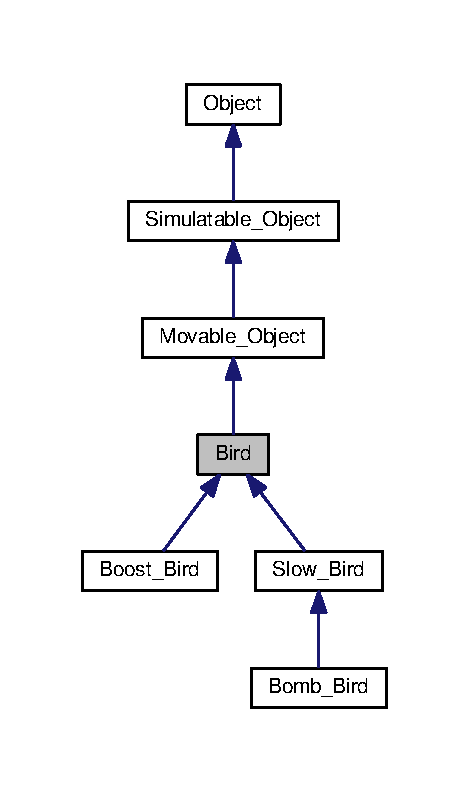
\includegraphics[width=226pt]{classBird__inherit__graph}
\end{center}
\end{figure}


Collaboration diagram for Bird\+:\nopagebreak
\begin{figure}[H]
\begin{center}
\leavevmode
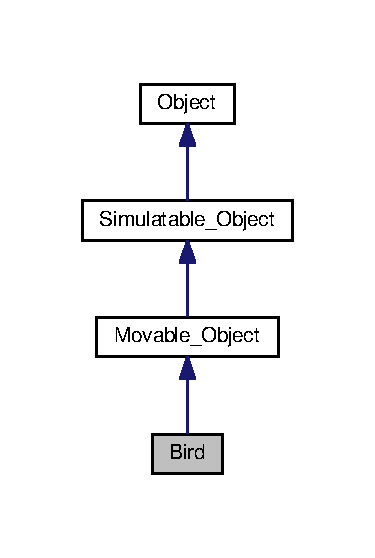
\includegraphics[width=180pt]{classBird__coll__graph}
\end{center}
\end{figure}
\subsection*{Public Member Functions}
\begin{DoxyCompactItemize}
\item 
\hyperlink{classBird_afe65295d7e648178245a1cd784924ecd}{Bird} (const sf\+::\+Vector2f \&, const sf\+::\+Vector2f \&, const std\+::string \&, const sf\+::\+Texture $\ast$, const float, const int, const float, const bool=false)
\begin{DoxyCompactList}\small\item\em \char`\"{}\+Constructor\char`\"{} \end{DoxyCompactList}\item 
virtual int \hyperlink{classBird_af2882ba302f03c5bdf5950cc21a39f66}{prepare\+\_\+simulate} (const float, const float) overridefinal
\begin{DoxyCompactList}\small\item\em \char`\"{}\+Prepares simulation of object\char`\"{} \end{DoxyCompactList}\end{DoxyCompactItemize}
\subsection*{Protected Member Functions}
\begin{DoxyCompactItemize}
\item 
\hypertarget{classBird_a3802ec1a4d2886ef8c95dd6d76038ab6}{virtual void {\bfseries handle\+\_\+moving\+\_\+collision} (const \hyperlink{classObject}{Object} $\ast$, const sf\+::\+Vector2f \&) overridefinal}\label{classBird_a3802ec1a4d2886ef8c95dd6d76038ab6}

\item 
\hypertarget{classBird_adbcfe9b09d3b828ce00982ec1aab9c6e}{virtual void {\bfseries handle\+\_\+static\+\_\+collision} (const \hyperlink{classObject}{Object} $\ast$)}\label{classBird_adbcfe9b09d3b828ce00982ec1aab9c6e}

\end{DoxyCompactItemize}
\subsection*{Protected Attributes}
\begin{DoxyCompactItemize}
\item 
\hypertarget{classBird_aad13ddaf4a6315ad3a2873e487cbc32b}{const float {\bfseries m\+\_\+speed}}\label{classBird_aad13ddaf4a6315ad3a2873e487cbc32b}

\item 
\hypertarget{classBird_a2e894d3d297ea72053ee319929c25f2c}{const float {\bfseries m\+\_\+cooldown}}\label{classBird_a2e894d3d297ea72053ee319929c25f2c}

\item 
\hypertarget{classBird_a2271962e5278b53dd7e600eea08465fc}{int {\bfseries m\+\_\+direction}}\label{classBird_a2271962e5278b53dd7e600eea08465fc}

\item 
\hypertarget{classBird_af212f094ae7b24978b494ef657ec9085}{sf\+::\+Clock {\bfseries m\+\_\+player\+\_\+clock}}\label{classBird_af212f094ae7b24978b494ef657ec9085}

\item 
\hypertarget{classBird_a0b43d6e0d01d780a18304731063897f6}{bool {\bfseries m\+\_\+player\+\_\+debuff} \{\}}\label{classBird_a0b43d6e0d01d780a18304731063897f6}

\end{DoxyCompactItemize}


\subsection{Constructor \& Destructor Documentation}
\hypertarget{classBird_afe65295d7e648178245a1cd784924ecd}{\index{Bird@{Bird}!Bird@{Bird}}
\index{Bird@{Bird}!Bird@{Bird}}
\subsubsection[{Bird}]{\setlength{\rightskip}{0pt plus 5cm}Bird\+::\+Bird (
\begin{DoxyParamCaption}
\item[{const sf\+::\+Vector2f \&}]{position, }
\item[{const sf\+::\+Vector2f \&}]{size, }
\item[{const std\+::string \&}]{type, }
\item[{const sf\+::\+Texture $\ast$}]{texture, }
\item[{const float}]{speed, }
\item[{const int}]{direction, }
\item[{const float}]{cooldown, }
\item[{const bool}]{solid = {\ttfamily false}}
\end{DoxyParamCaption}
)}}\label{classBird_afe65295d7e648178245a1cd784924ecd}


\char`\"{}\+Constructor\char`\"{} 


\begin{DoxyParams}{Parameters}
{\em position} & \char`\"{}\+Position of the object\char`\"{} \\
\hline
{\em size} & \char`\"{}\+Size of the object\char`\"{} \\
\hline
{\em type} & \char`\"{}\+Type of the object\char`\"{} \\
\hline
{\em texture} & \char`\"{}\+Texture of the object\char`\"{} \\
\hline
{\em speed} & \char`\"{}\+Speed of the object\char`\"{} \\
\hline
{\em direction} & \char`\"{}\+Direction of the object\char`\"{} \\
\hline
{\em cooldown} & \char`\"{}\+How long the objects opacity is 0.\+5\char`\"{} \\
\hline
{\em solid} & \char`\"{}\+If the object is solid\char`\"{} \\
\hline
\end{DoxyParams}


\subsection{Member Function Documentation}
\hypertarget{classBird_af2882ba302f03c5bdf5950cc21a39f66}{\index{Bird@{Bird}!prepare\+\_\+simulate@{prepare\+\_\+simulate}}
\index{prepare\+\_\+simulate@{prepare\+\_\+simulate}!Bird@{Bird}}
\subsubsection[{prepare\+\_\+simulate}]{\setlength{\rightskip}{0pt plus 5cm}int Bird\+::prepare\+\_\+simulate (
\begin{DoxyParamCaption}
\item[{const float}]{distance\+\_\+modifier, }
\item[{const float}]{}
\end{DoxyParamCaption}
)\hspace{0.3cm}{\ttfamily [final]}, {\ttfamily [override]}, {\ttfamily [virtual]}}}\label{classBird_af2882ba302f03c5bdf5950cc21a39f66}


\char`\"{}\+Prepares simulation of object\char`\"{} 


\begin{DoxyParams}{Parameters}
{\em distance\+\_\+modifier} & \char`\"{}\+Delta since last simulation-\/sequence\char`\"{} \\
\hline
{\em gravity\+\_\+constant} & \char`\"{}\+How much high the gravity is\char`\"{} \\
\hline
\end{DoxyParams}
\begin{DoxyReturn}{Returns}
\char`\"{}\+Simulation cycles required by this object this simulation-\/sequence\char`\"{} 
\end{DoxyReturn}


Implements \hyperlink{classSimulatable__Object_abe7c02fe250ef5be42011890d8a7b37b}{Simulatable\+\_\+\+Object}.



The documentation for this class was generated from the following files\+:\begin{DoxyCompactItemize}
\item 
objects/abstractish/bird.\+h\item 
objects/abstractish/bird.\+cc\end{DoxyCompactItemize}

\hypertarget{classBomb__Bird}{\section{Bomb\+\_\+\+Bird Class Reference}
\label{classBomb__Bird}\index{Bomb\+\_\+\+Bird@{Bomb\+\_\+\+Bird}}
}


Inheritance diagram for Bomb\+\_\+\+Bird\+:\nopagebreak
\begin{figure}[H]
\begin{center}
\leavevmode
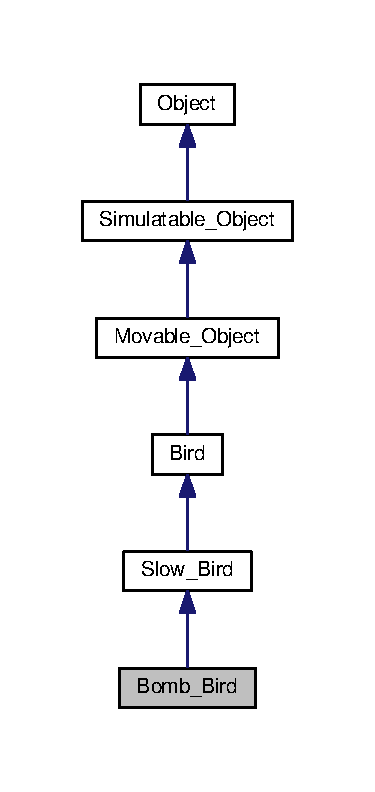
\includegraphics[width=180pt]{classBomb__Bird__inherit__graph}
\end{center}
\end{figure}


Collaboration diagram for Bomb\+\_\+\+Bird\+:\nopagebreak
\begin{figure}[H]
\begin{center}
\leavevmode
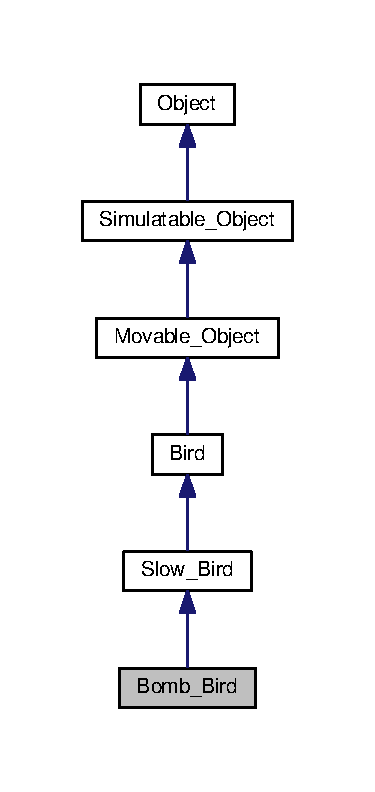
\includegraphics[width=180pt]{classBomb__Bird__coll__graph}
\end{center}
\end{figure}
\subsection*{Public Member Functions}
\begin{DoxyCompactItemize}
\item 
\hyperlink{classBomb__Bird_a920e7058e7cff86be951c2b9feede80e}{Bomb\+\_\+\+Bird} (const sf\+::\+Vector2f \&, const sf\+::\+Vector2f \&, const std\+::string \&, const sf\+::\+Texture $\ast$, const float, const int, const sf\+::\+Texture $\ast$)
\begin{DoxyCompactList}\small\item\em \char`\"{}\+Constructor\char`\"{} \end{DoxyCompactList}\item 
virtual std\+::vector$<$ \hyperlink{classObject}{Object} $\ast$ $>$ \hyperlink{classBomb__Bird_a610b4c68c560a6ac30375c177642e021}{simulate} (const int, const std\+::vector$<$ const \hyperlink{classObject}{Object} $\ast$ $>$ \&) overridefinal
\begin{DoxyCompactList}\small\item\em \char`\"{}\+Executes simulation of object\char`\"{} \end{DoxyCompactList}\end{DoxyCompactItemize}
\subsection*{Additional Inherited Members}


\subsection{Constructor \& Destructor Documentation}
\hypertarget{classBomb__Bird_a920e7058e7cff86be951c2b9feede80e}{\index{Bomb\+\_\+\+Bird@{Bomb\+\_\+\+Bird}!Bomb\+\_\+\+Bird@{Bomb\+\_\+\+Bird}}
\index{Bomb\+\_\+\+Bird@{Bomb\+\_\+\+Bird}!Bomb\+\_\+\+Bird@{Bomb\+\_\+\+Bird}}
\subsubsection[{Bomb\+\_\+\+Bird}]{\setlength{\rightskip}{0pt plus 5cm}Bomb\+\_\+\+Bird\+::\+Bomb\+\_\+\+Bird (
\begin{DoxyParamCaption}
\item[{const sf\+::\+Vector2f \&}]{position, }
\item[{const sf\+::\+Vector2f \&}]{size, }
\item[{const std\+::string \&}]{type, }
\item[{const sf\+::\+Texture $\ast$}]{texture, }
\item[{const float}]{speed, }
\item[{const int}]{direction, }
\item[{const sf\+::\+Texture $\ast$}]{nfbb\+\_\+texture}
\end{DoxyParamCaption}
)}}\label{classBomb__Bird_a920e7058e7cff86be951c2b9feede80e}


\char`\"{}\+Constructor\char`\"{} 


\begin{DoxyParams}{Parameters}
{\em position} & \char`\"{}\+Position of the object\char`\"{} \\
\hline
{\em size} & \char`\"{}\+Size of the object\char`\"{} \\
\hline
{\em type} & \char`\"{}\+Type of the object\char`\"{} \\
\hline
{\em texture} & \char`\"{}\+Texture of the object\char`\"{} \\
\hline
{\em speed} & \char`\"{}\+Speed of the object\char`\"{} \\
\hline
{\em direction} & \char`\"{}\+Direction of the object\char`\"{} \\
\hline
{\em nfbb\+\_\+texture} & \char`\"{}\+Texture of N\+F\+B\+B-\/objects spawned by the object\char`\"{} \\
\hline
\end{DoxyParams}


\subsection{Member Function Documentation}
\hypertarget{classBomb__Bird_a610b4c68c560a6ac30375c177642e021}{\index{Bomb\+\_\+\+Bird@{Bomb\+\_\+\+Bird}!simulate@{simulate}}
\index{simulate@{simulate}!Bomb\+\_\+\+Bird@{Bomb\+\_\+\+Bird}}
\subsubsection[{simulate}]{\setlength{\rightskip}{0pt plus 5cm}std\+::vector$<$ {\bf Object} $\ast$ $>$ Bomb\+\_\+\+Bird\+::simulate (
\begin{DoxyParamCaption}
\item[{const int}]{simulation\+\_\+cycles, }
\item[{const std\+::vector$<$ const {\bf Object} $\ast$ $>$ \&}]{objects}
\end{DoxyParamCaption}
)\hspace{0.3cm}{\ttfamily [final]}, {\ttfamily [override]}, {\ttfamily [virtual]}}}\label{classBomb__Bird_a610b4c68c560a6ac30375c177642e021}


\char`\"{}\+Executes simulation of object\char`\"{} 


\begin{DoxyParams}{Parameters}
{\em simulation\+\_\+cycles} & \char`\"{}\+Number simulation\+\_\+cycles the object will be subjected this simulation-\/sequence\char`\"{} \\
\hline
{\em objects} & \char`\"{}\+Objects to check for collision with\char`\"{} \\
\hline
\end{DoxyParams}
\begin{DoxyReturn}{Returns}
\char`\"{}\+New objects spawned by this object\char`\"{} 
\end{DoxyReturn}


Reimplemented from \hyperlink{classMovable__Object_ac267e0c945b558b0cf533d7fbe5ee7c3}{Movable\+\_\+\+Object}.



The documentation for this class was generated from the following files\+:\begin{DoxyCompactItemize}
\item 
objects/non\+\_\+abstract/bomb\+\_\+bird.\+h\item 
objects/non\+\_\+abstract/bomb\+\_\+bird.\+cc\end{DoxyCompactItemize}

\hypertarget{classBoost__Bird}{\section{Boost\+\_\+\+Bird Class Reference}
\label{classBoost__Bird}\index{Boost\+\_\+\+Bird@{Boost\+\_\+\+Bird}}
}


Inheritance diagram for Boost\+\_\+\+Bird\+:\nopagebreak
\begin{figure}[H]
\begin{center}
\leavevmode
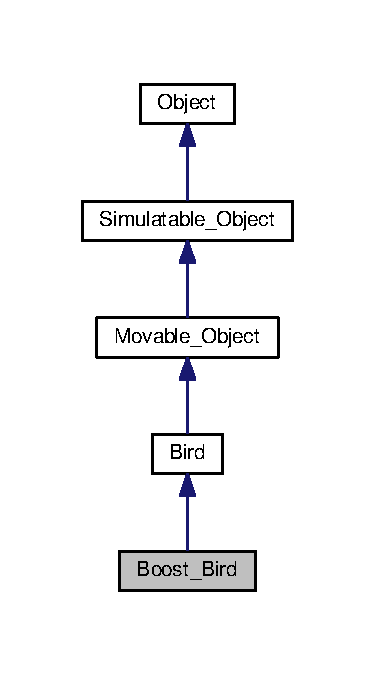
\includegraphics[width=180pt]{classBoost__Bird__inherit__graph}
\end{center}
\end{figure}


Collaboration diagram for Boost\+\_\+\+Bird\+:\nopagebreak
\begin{figure}[H]
\begin{center}
\leavevmode
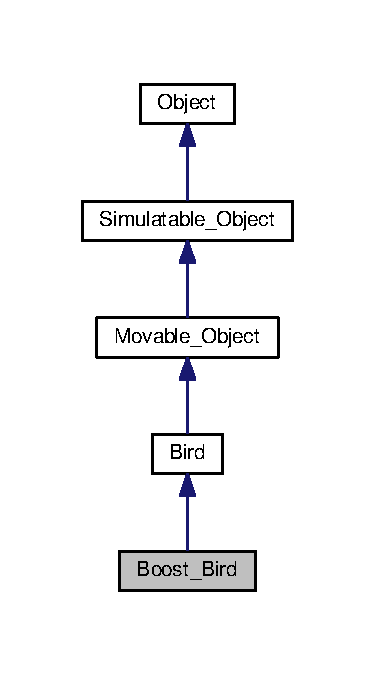
\includegraphics[width=180pt]{classBoost__Bird__coll__graph}
\end{center}
\end{figure}
\subsection*{Public Member Functions}
\begin{DoxyCompactItemize}
\item 
\hyperlink{classBoost__Bird_a03587afcb2e53cde2116d03d05f99846}{Boost\+\_\+\+Bird} (const sf\+::\+Vector2f \&, const sf\+::\+Vector2f \&, const std\+::string \&, const sf\+::\+Texture $\ast$, const float, const int)
\begin{DoxyCompactList}\small\item\em \char`\"{}\+Constructor\char`\"{} \end{DoxyCompactList}\end{DoxyCompactItemize}
\subsection*{Additional Inherited Members}


\subsection{Constructor \& Destructor Documentation}
\hypertarget{classBoost__Bird_a03587afcb2e53cde2116d03d05f99846}{\index{Boost\+\_\+\+Bird@{Boost\+\_\+\+Bird}!Boost\+\_\+\+Bird@{Boost\+\_\+\+Bird}}
\index{Boost\+\_\+\+Bird@{Boost\+\_\+\+Bird}!Boost\+\_\+\+Bird@{Boost\+\_\+\+Bird}}
\subsubsection[{Boost\+\_\+\+Bird}]{\setlength{\rightskip}{0pt plus 5cm}Boost\+\_\+\+Bird\+::\+Boost\+\_\+\+Bird (
\begin{DoxyParamCaption}
\item[{const sf\+::\+Vector2f \&}]{position, }
\item[{const sf\+::\+Vector2f \&}]{size, }
\item[{const std\+::string \&}]{type, }
\item[{const sf\+::\+Texture $\ast$}]{texture, }
\item[{const float}]{speed, }
\item[{const int}]{direction}
\end{DoxyParamCaption}
)}}\label{classBoost__Bird_a03587afcb2e53cde2116d03d05f99846}


\char`\"{}\+Constructor\char`\"{} 


\begin{DoxyParams}{Parameters}
{\em position} & \char`\"{}\+Position of the object\char`\"{} \\
\hline
{\em size} & \char`\"{}\+Size of the object\char`\"{} \\
\hline
{\em type} & \char`\"{}\+Type of the object\char`\"{} \\
\hline
{\em texture} & \char`\"{}\+Texture of the object\char`\"{} \\
\hline
{\em speed} & \char`\"{}\+Speed of the object\char`\"{} \\
\hline
{\em direction} & \char`\"{}\+Direction of the object\char`\"{} \\
\hline
\end{DoxyParams}


The documentation for this class was generated from the following files\+:\begin{DoxyCompactItemize}
\item 
objects/non\+\_\+abstract/boost\+\_\+bird.\+h\item 
objects/non\+\_\+abstract/boost\+\_\+bird.\+cc\end{DoxyCompactItemize}

\hypertarget{structdocument__order__comparator}{\section{document\+\_\+order\+\_\+comparator Struct Reference}
\label{structdocument__order__comparator}\index{document\+\_\+order\+\_\+comparator@{document\+\_\+order\+\_\+comparator}}
}
\subsection*{Public Member Functions}
\begin{DoxyCompactItemize}
\item 
\hypertarget{structdocument__order__comparator_a11e471cbfa426bc9e48844c1db1a190e}{bool {\bfseries operator()} (const xpath\+\_\+node \&lhs, const xpath\+\_\+node \&rhs) const }\label{structdocument__order__comparator_a11e471cbfa426bc9e48844c1db1a190e}

\end{DoxyCompactItemize}


The documentation for this struct was generated from the following file\+:\begin{DoxyCompactItemize}
\item 
resources/pugixml-\/1.\+8/src/pugixml.\+cpp\end{DoxyCompactItemize}

\hypertarget{structduplicate__comparator}{\section{duplicate\+\_\+comparator Struct Reference}
\label{structduplicate__comparator}\index{duplicate\+\_\+comparator@{duplicate\+\_\+comparator}}
}
\subsection*{Public Member Functions}
\begin{DoxyCompactItemize}
\item 
\hypertarget{structduplicate__comparator_afa36b2cf7af3e0bc7e41b03995bd99d3}{bool {\bfseries operator()} (const xpath\+\_\+node \&lhs, const xpath\+\_\+node \&rhs) const }\label{structduplicate__comparator_afa36b2cf7af3e0bc7e41b03995bd99d3}

\end{DoxyCompactItemize}


The documentation for this struct was generated from the following file\+:\begin{DoxyCompactItemize}
\item 
resources/pugixml-\/1.\+8/src/pugixml.\+cpp\end{DoxyCompactItemize}

\hypertarget{classEngine}{\section{Engine Class Reference}
\label{classEngine}\index{Engine@{Engine}}
}
\subsection*{Public Member Functions}
\begin{DoxyCompactItemize}
\item 
\hypertarget{classEngine_a8c98683b0a3aa28d8ab72a8bcd0d52f2}{\hyperlink{classEngine_a8c98683b0a3aa28d8ab72a8bcd0d52f2}{Engine} ()}\label{classEngine_a8c98683b0a3aa28d8ab72a8bcd0d52f2}

\begin{DoxyCompactList}\small\item\em \char`\"{}\+Constructor \+: creates State-\/objects and view,
        as well as setting the active-\/state and prepares it for simulation\char`\"{} \end{DoxyCompactList}\item 
\hypertarget{classEngine_a8ef7030a089ecb30bbfcb9e43094717a}{\hyperlink{classEngine_a8ef7030a089ecb30bbfcb9e43094717a}{$\sim$\+Engine} ()}\label{classEngine_a8ef7030a089ecb30bbfcb9e43094717a}

\begin{DoxyCompactList}\small\item\em \char`\"{}\+Destructor \+: frees resources owned by the Engine\char`\"{} \end{DoxyCompactList}\item 
void \hyperlink{classEngine_abedfd6c2327693f468b710bd79a9fe4c}{simulate} (sf\+::\+Render\+Window \&)
\begin{DoxyCompactList}\small\item\em \char`\"{}\+Simulates the active state, and, depending on the return value
       from the simulation, might change the active-\/state or close the window\char`\"{} \end{DoxyCompactList}\item 
void \hyperlink{classEngine_a4d9a19bdf6a13b84570e400acab6de6c}{render} (sf\+::\+Render\+Window \&)
\begin{DoxyCompactList}\small\item\em \char`\"{}draws all texturated objects and text objects in the active state\char`\"{} \end{DoxyCompactList}\end{DoxyCompactItemize}


\subsection{Member Function Documentation}
\hypertarget{classEngine_a4d9a19bdf6a13b84570e400acab6de6c}{\index{Engine@{Engine}!render@{render}}
\index{render@{render}!Engine@{Engine}}
\subsubsection[{render}]{\setlength{\rightskip}{0pt plus 5cm}void Engine\+::render (
\begin{DoxyParamCaption}
\item[{sf\+::\+Render\+Window \&}]{window}
\end{DoxyParamCaption}
)}}\label{classEngine_a4d9a19bdf6a13b84570e400acab6de6c}


\char`\"{}draws all texturated objects and text objects in the active state\char`\"{} 


\begin{DoxyParams}{Parameters}
{\em window} & \char`\"{}window draw on\char`\"{} \\
\hline
\end{DoxyParams}
\hypertarget{classEngine_abedfd6c2327693f468b710bd79a9fe4c}{\index{Engine@{Engine}!simulate@{simulate}}
\index{simulate@{simulate}!Engine@{Engine}}
\subsubsection[{simulate}]{\setlength{\rightskip}{0pt plus 5cm}void Engine\+::simulate (
\begin{DoxyParamCaption}
\item[{sf\+::\+Render\+Window \&}]{window}
\end{DoxyParamCaption}
)}}\label{classEngine_abedfd6c2327693f468b710bd79a9fe4c}


\char`\"{}\+Simulates the active state, and, depending on the return value
       from the simulation, might change the active-\/state or close the window\char`\"{} 


\begin{DoxyParams}{Parameters}
{\em window} & \char`\"{}window to close\char`\"{} \\
\hline
\end{DoxyParams}


The documentation for this class was generated from the following files\+:\begin{DoxyCompactItemize}
\item 
engine/engine.\+h\item 
engine/engine.\+cc\end{DoxyCompactItemize}

\hypertarget{structequal__to}{\section{equal\+\_\+to Struct Reference}
\label{structequal__to}\index{equal\+\_\+to@{equal\+\_\+to}}
}
\subsection*{Public Member Functions}
\begin{DoxyCompactItemize}
\item 
\hypertarget{structequal__to_acaf39da83a307280fef2f11691386b0e}{{\footnotesize template$<$typename T $>$ }\\bool {\bfseries operator()} (const T \&lhs, const T \&rhs) const }\label{structequal__to_acaf39da83a307280fef2f11691386b0e}

\end{DoxyCompactItemize}


The documentation for this struct was generated from the following file\+:\begin{DoxyCompactItemize}
\item 
resources/pugixml-\/1.\+8/src/pugixml.\+cpp\end{DoxyCompactItemize}

\hypertarget{classGame__State}{\section{Game\+\_\+\+State Class Reference}
\label{classGame__State}\index{Game\+\_\+\+State@{Game\+\_\+\+State}}
}


Inheritance diagram for Game\+\_\+\+State\+:\nopagebreak
\begin{figure}[H]
\begin{center}
\leavevmode
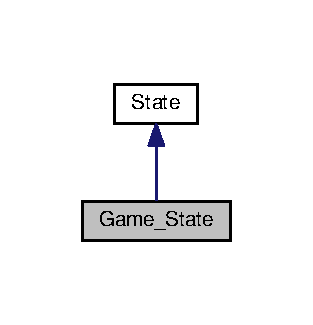
\includegraphics[width=150pt]{classGame__State__inherit__graph}
\end{center}
\end{figure}


Collaboration diagram for Game\+\_\+\+State\+:\nopagebreak
\begin{figure}[H]
\begin{center}
\leavevmode
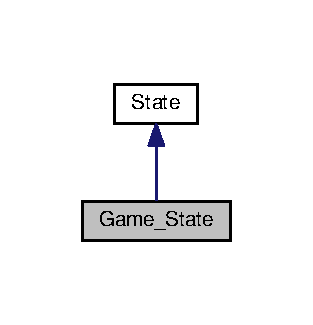
\includegraphics[width=150pt]{classGame__State__coll__graph}
\end{center}
\end{figure}
\subsection*{Public Member Functions}
\begin{DoxyCompactItemize}
\item 
\hypertarget{classGame__State_a8104ef051de61662ee5aef3f63c5d331}{\hyperlink{classGame__State_a8104ef051de61662ee5aef3f63c5d331}{Game\+\_\+\+State} ()}\label{classGame__State_a8104ef051de61662ee5aef3f63c5d331}

\begin{DoxyCompactList}\small\item\em \char`\"{}\+Constructor \+: loads all textures and fonts used in the state\char`\"{} \end{DoxyCompactList}\item 
\hypertarget{classGame__State_a9ad8826703bd8aff5bfeaba29b25e296}{void \hyperlink{classGame__State_a9ad8826703bd8aff5bfeaba29b25e296}{prepare\+\_\+simulate} () override}\label{classGame__State_a9ad8826703bd8aff5bfeaba29b25e296}

\begin{DoxyCompactList}\small\item\em \char`\"{}\+Resets the state and loads a new level into it with the help
        of the Level Parser class\char`\"{} \end{DoxyCompactList}\item 
int \hyperlink{classGame__State_ab45e81cb4c422cd23cd245cd3fb9c87f}{simulate} () override
\begin{DoxyCompactList}\small\item\em \char`\"{}\+Simulates each object in the state and performs actions on
        the state based on the result of the simulations\char`\"{} \end{DoxyCompactList}\item 
void \hyperlink{classGame__State_a1a24aa350628b7f3005e56c5efaadad7}{set\+\_\+view} (sf\+::\+View \&) override
\begin{DoxyCompactList}\small\item\em \char`\"{}\+Centers the view around the player\char`\"{} \end{DoxyCompactList}\end{DoxyCompactItemize}
\subsection*{Additional Inherited Members}


\subsection{Member Function Documentation}
\hypertarget{classGame__State_a1a24aa350628b7f3005e56c5efaadad7}{\index{Game\+\_\+\+State@{Game\+\_\+\+State}!set\+\_\+view@{set\+\_\+view}}
\index{set\+\_\+view@{set\+\_\+view}!Game\+\_\+\+State@{Game\+\_\+\+State}}
\subsubsection[{set\+\_\+view}]{\setlength{\rightskip}{0pt plus 5cm}void Game\+\_\+\+State\+::set\+\_\+view (
\begin{DoxyParamCaption}
\item[{sf\+::\+View \&}]{view}
\end{DoxyParamCaption}
)\hspace{0.3cm}{\ttfamily [override]}, {\ttfamily [virtual]}}}\label{classGame__State_a1a24aa350628b7f3005e56c5efaadad7}


\char`\"{}\+Centers the view around the player\char`\"{} 


\begin{DoxyParams}{Parameters}
{\em view} & \char`\"{}\+View to perform action on\char`\"{} \\
\hline
\end{DoxyParams}


Implements \hyperlink{classState}{State}.

\hypertarget{classGame__State_ab45e81cb4c422cd23cd245cd3fb9c87f}{\index{Game\+\_\+\+State@{Game\+\_\+\+State}!simulate@{simulate}}
\index{simulate@{simulate}!Game\+\_\+\+State@{Game\+\_\+\+State}}
\subsubsection[{simulate}]{\setlength{\rightskip}{0pt plus 5cm}int Game\+\_\+\+State\+::simulate (
\begin{DoxyParamCaption}
{}
\end{DoxyParamCaption}
)\hspace{0.3cm}{\ttfamily [override]}, {\ttfamily [virtual]}}}\label{classGame__State_ab45e81cb4c422cd23cd245cd3fb9c87f}


\char`\"{}\+Simulates each object in the state and performs actions on
        the state based on the result of the simulations\char`\"{} 

\begin{DoxyReturn}{Returns}
\char`\"{}\+An integer representing the next action to be taken by the Engine object\char`\"{} 
\end{DoxyReturn}


Implements \hyperlink{classState}{State}.



The documentation for this class was generated from the following files\+:\begin{DoxyCompactItemize}
\item 
states/non\+\_\+abstract/game\+\_\+state.\+h\item 
states/non\+\_\+abstract/game\+\_\+state.\+cc\end{DoxyCompactItemize}

\hypertarget{structgap}{\section{gap Struct Reference}
\label{structgap}\index{gap@{gap}}
}
\subsection*{Public Member Functions}
\begin{DoxyCompactItemize}
\item 
\hypertarget{structgap_a9c0d0b12bc778c8439c8aec7747ab2b0}{void {\bfseries push} (char\+\_\+t $\ast$\&s, size\+\_\+t count)}\label{structgap_a9c0d0b12bc778c8439c8aec7747ab2b0}

\item 
\hypertarget{structgap_a176c58ee8d57c41b91ae9f00d5e8cab5}{char\+\_\+t $\ast$ {\bfseries flush} (char\+\_\+t $\ast$s)}\label{structgap_a176c58ee8d57c41b91ae9f00d5e8cab5}

\end{DoxyCompactItemize}
\subsection*{Public Attributes}
\begin{DoxyCompactItemize}
\item 
\hypertarget{structgap_a1fafd4d9909a3413f723f24e46dfde0e}{char\+\_\+t $\ast$ {\bfseries end}}\label{structgap_a1fafd4d9909a3413f723f24e46dfde0e}

\item 
\hypertarget{structgap_ad5bb3597ade78d89bbe0e300748ad508}{size\+\_\+t {\bfseries size}}\label{structgap_ad5bb3597ade78d89bbe0e300748ad508}

\end{DoxyCompactItemize}


The documentation for this struct was generated from the following file\+:\begin{DoxyCompactItemize}
\item 
resources/pugixml-\/1.\+8/src/pugixml.\+cpp\end{DoxyCompactItemize}

\hypertarget{classGravitating__Object}{\section{Gravitating\+\_\+\+Object Class Reference}
\label{classGravitating__Object}\index{Gravitating\+\_\+\+Object@{Gravitating\+\_\+\+Object}}
}


Inheritance diagram for Gravitating\+\_\+\+Object\+:\nopagebreak
\begin{figure}[H]
\begin{center}
\leavevmode
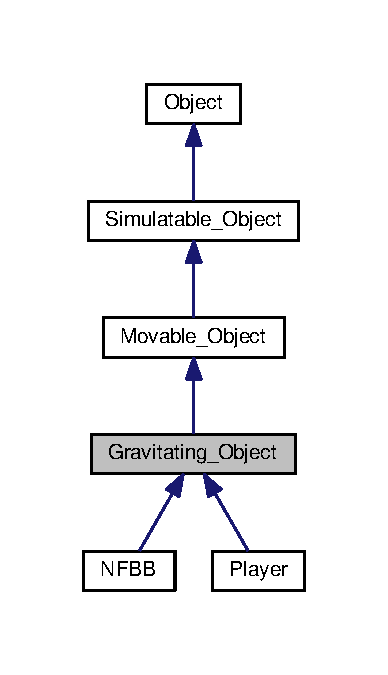
\includegraphics[width=186pt]{classGravitating__Object__inherit__graph}
\end{center}
\end{figure}


Collaboration diagram for Gravitating\+\_\+\+Object\+:\nopagebreak
\begin{figure}[H]
\begin{center}
\leavevmode
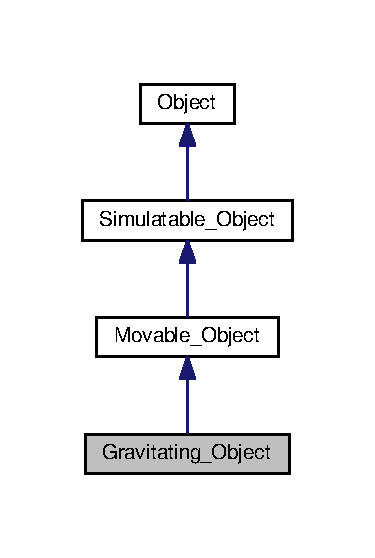
\includegraphics[width=180pt]{classGravitating__Object__coll__graph}
\end{center}
\end{figure}
\subsection*{Public Member Functions}
\begin{DoxyCompactItemize}
\item 
\hyperlink{classGravitating__Object_a7319a97eb2d84afbe66c5e0040bd3973}{Gravitating\+\_\+\+Object} (const sf\+::\+Vector2f \&, const sf\+::\+Vector2f \&, const std\+::string \&, const bool=false, const sf\+::\+Texture $\ast$=nullptr)
\begin{DoxyCompactList}\small\item\em \char`\"{}\+Constructor\char`\"{} \end{DoxyCompactList}\item 
int \hyperlink{classGravitating__Object_a187404d6df6ff16a86a33a3f4a8aab85}{prepare\+\_\+simulate} (const float, const float)
\begin{DoxyCompactList}\small\item\em \char`\"{}\+Prepares simulation of object\char`\"{} \end{DoxyCompactList}\end{DoxyCompactItemize}
\subsection*{Protected Member Functions}
\begin{DoxyCompactItemize}
\item 
\hypertarget{classGravitating__Object_ad059f059b3699edb3edff11fdd7fba29}{virtual void {\bfseries handle\+\_\+moving\+\_\+collision} (const \hyperlink{classObject}{Object} $\ast$, const sf\+::\+Vector2f \&) override}\label{classGravitating__Object_ad059f059b3699edb3edff11fdd7fba29}

\end{DoxyCompactItemize}
\subsection*{Protected Attributes}
\begin{DoxyCompactItemize}
\item 
\hypertarget{classGravitating__Object_abda4e488702c931d99b47785db6be33b}{sf\+::\+Clock {\bfseries m\+\_\+gravity\+\_\+clock}}\label{classGravitating__Object_abda4e488702c931d99b47785db6be33b}

\end{DoxyCompactItemize}


\subsection{Constructor \& Destructor Documentation}
\hypertarget{classGravitating__Object_a7319a97eb2d84afbe66c5e0040bd3973}{\index{Gravitating\+\_\+\+Object@{Gravitating\+\_\+\+Object}!Gravitating\+\_\+\+Object@{Gravitating\+\_\+\+Object}}
\index{Gravitating\+\_\+\+Object@{Gravitating\+\_\+\+Object}!Gravitating\+\_\+\+Object@{Gravitating\+\_\+\+Object}}
\subsubsection[{Gravitating\+\_\+\+Object}]{\setlength{\rightskip}{0pt plus 5cm}Gravitating\+\_\+\+Object\+::\+Gravitating\+\_\+\+Object (
\begin{DoxyParamCaption}
\item[{const sf\+::\+Vector2f \&}]{position, }
\item[{const sf\+::\+Vector2f \&}]{size, }
\item[{const std\+::string \&}]{type, }
\item[{const bool}]{solid = {\ttfamily false}, }
\item[{const sf\+::\+Texture $\ast$}]{texture = {\ttfamily nullptr}}
\end{DoxyParamCaption}
)}}\label{classGravitating__Object_a7319a97eb2d84afbe66c5e0040bd3973}


\char`\"{}\+Constructor\char`\"{} 


\begin{DoxyParams}{Parameters}
{\em position} & \char`\"{}\+Position of the object\char`\"{} \\
\hline
{\em size} & \char`\"{}\+Size of the object\char`\"{} \\
\hline
{\em type} & \char`\"{}\+Type of the object\char`\"{} \\
\hline
{\em solid} & \char`\"{}\+If the object is solid\char`\"{} \\
\hline
{\em texture} & \char`\"{}\+Texture of the object\char`\"{}" \\
\hline
\end{DoxyParams}


\subsection{Member Function Documentation}
\hypertarget{classGravitating__Object_a187404d6df6ff16a86a33a3f4a8aab85}{\index{Gravitating\+\_\+\+Object@{Gravitating\+\_\+\+Object}!prepare\+\_\+simulate@{prepare\+\_\+simulate}}
\index{prepare\+\_\+simulate@{prepare\+\_\+simulate}!Gravitating\+\_\+\+Object@{Gravitating\+\_\+\+Object}}
\subsubsection[{prepare\+\_\+simulate}]{\setlength{\rightskip}{0pt plus 5cm}int Gravitating\+\_\+\+Object\+::prepare\+\_\+simulate (
\begin{DoxyParamCaption}
\item[{const float}]{distance\+\_\+modifier, }
\item[{const float}]{gravity\+\_\+constant}
\end{DoxyParamCaption}
)\hspace{0.3cm}{\ttfamily [virtual]}}}\label{classGravitating__Object_a187404d6df6ff16a86a33a3f4a8aab85}


\char`\"{}\+Prepares simulation of object\char`\"{} 


\begin{DoxyParams}{Parameters}
{\em distance\+\_\+modifier} & \char`\"{}\+Delta since last simulation-\/sequence\char`\"{} \\
\hline
{\em gravity\+\_\+constant} & \char`\"{}\+How much high the gravity is\char`\"{} \\
\hline
\end{DoxyParams}
\begin{DoxyReturn}{Returns}
\char`\"{}\+Simulation cycles required by this object this simulation-\/sequence\char`\"{} 
\end{DoxyReturn}


Implements \hyperlink{classSimulatable__Object_abe7c02fe250ef5be42011890d8a7b37b}{Simulatable\+\_\+\+Object}.



Reimplemented in \hyperlink{classPlayer_a1480bbfb767687380ad6a2bf294cdcc8}{Player}.



The documentation for this class was generated from the following files\+:\begin{DoxyCompactItemize}
\item 
objects/abstractish/gravitating\+\_\+object.\+h\item 
objects/abstractish/gravitating\+\_\+object.\+cc\end{DoxyCompactItemize}

\hypertarget{structlatin1__decoder}{\section{latin1\+\_\+decoder Struct Reference}
\label{structlatin1__decoder}\index{latin1\+\_\+decoder@{latin1\+\_\+decoder}}
}
\subsection*{Public Types}
\begin{DoxyCompactItemize}
\item 
\hypertarget{structlatin1__decoder_a8eec1209fbcf34e5a8fe7bfc082f9c1b}{typedef uint8\+\_\+t {\bfseries type}}\label{structlatin1__decoder_a8eec1209fbcf34e5a8fe7bfc082f9c1b}

\end{DoxyCompactItemize}
\subsection*{Static Public Member Functions}
\begin{DoxyCompactItemize}
\item 
\hypertarget{structlatin1__decoder_acf3e6f85693d539919dec3bfb9cee66f}{{\footnotesize template$<$typename Traits $>$ }\\static Traits\+::value\+\_\+type {\bfseries process} (const uint8\+\_\+t $\ast$data, size\+\_\+t size, typename Traits\+::value\+\_\+type result, Traits)}\label{structlatin1__decoder_acf3e6f85693d539919dec3bfb9cee66f}

\end{DoxyCompactItemize}


The documentation for this struct was generated from the following file\+:\begin{DoxyCompactItemize}
\item 
resources/pugixml-\/1.\+8/src/pugixml.\+cpp\end{DoxyCompactItemize}

\hypertarget{structlatin1__writer}{\section{latin1\+\_\+writer Struct Reference}
\label{structlatin1__writer}\index{latin1\+\_\+writer@{latin1\+\_\+writer}}
}
\subsection*{Public Types}
\begin{DoxyCompactItemize}
\item 
\hypertarget{structlatin1__writer_af9228600fa7eecd793cc3d927d46eb1a}{typedef uint8\+\_\+t $\ast$ {\bfseries value\+\_\+type}}\label{structlatin1__writer_af9228600fa7eecd793cc3d927d46eb1a}

\end{DoxyCompactItemize}
\subsection*{Static Public Member Functions}
\begin{DoxyCompactItemize}
\item 
\hypertarget{structlatin1__writer_ab5d7a833d29d66031420686ca67b1f6e}{static value\+\_\+type {\bfseries low} (value\+\_\+type result, uint32\+\_\+t ch)}\label{structlatin1__writer_ab5d7a833d29d66031420686ca67b1f6e}

\item 
\hypertarget{structlatin1__writer_a0e48c306ebe556f267404a9624f00554}{static value\+\_\+type {\bfseries high} (value\+\_\+type result, uint32\+\_\+t ch)}\label{structlatin1__writer_a0e48c306ebe556f267404a9624f00554}

\end{DoxyCompactItemize}


The documentation for this struct was generated from the following file\+:\begin{DoxyCompactItemize}
\item 
resources/pugixml-\/1.\+8/src/pugixml.\+cpp\end{DoxyCompactItemize}

\hypertarget{structless}{\section{less Struct Reference}
\label{structless}\index{less@{less}}
}
\subsection*{Public Member Functions}
\begin{DoxyCompactItemize}
\item 
\hypertarget{structless_ad467675b44baab18215475c7cba0cb48}{{\footnotesize template$<$typename T $>$ }\\bool {\bfseries operator()} (const T \&lhs, const T \&rhs) const }\label{structless_ad467675b44baab18215475c7cba0cb48}

\end{DoxyCompactItemize}


The documentation for this struct was generated from the following file\+:\begin{DoxyCompactItemize}
\item 
resources/pugixml-\/1.\+8/src/pugixml.\+cpp\end{DoxyCompactItemize}

\hypertarget{structless__equal}{\section{less\+\_\+equal Struct Reference}
\label{structless__equal}\index{less\+\_\+equal@{less\+\_\+equal}}
}
\subsection*{Public Member Functions}
\begin{DoxyCompactItemize}
\item 
\hypertarget{structless__equal_a88d7a445c55ca234e3595aa086ff6a7d}{{\footnotesize template$<$typename T $>$ }\\bool {\bfseries operator()} (const T \&lhs, const T \&rhs) const }\label{structless__equal_a88d7a445c55ca234e3595aa086ff6a7d}

\end{DoxyCompactItemize}


The documentation for this struct was generated from the following file\+:\begin{DoxyCompactItemize}
\item 
resources/pugixml-\/1.\+8/src/pugixml.\+cpp\end{DoxyCompactItemize}

\hypertarget{classLevel__Parser}{\section{Level\+\_\+\+Parser Class Reference}
\label{classLevel__Parser}\index{Level\+\_\+\+Parser@{Level\+\_\+\+Parser}}
}
\subsection*{Public Member Functions}
\begin{DoxyCompactItemize}
\item 
\hyperlink{classLevel__Parser_ac1e8138a19ac3d284010c693e5ca446c}{Level\+\_\+\+Parser} (const std\+::string \&)
\begin{DoxyCompactList}\small\item\em \char`\"{}\+Constructor\char`\"{} \end{DoxyCompactList}\item 
std\+::vector$<$ \hyperlink{classObject}{Object} $\ast$ $>$ \hyperlink{classLevel__Parser_af3206216900aae52b79289c3f75c1e32}{get\+\_\+objects} (const std\+::unordered\+\_\+map$<$ std\+::string, sf\+::\+Texture $\ast$ $>$ \&) const 
\begin{DoxyCompactList}\small\item\em \char`\"{}\+Creates and returns all objects in loaded file\char`\"{} \end{DoxyCompactList}\end{DoxyCompactItemize}


\subsection{Constructor \& Destructor Documentation}
\hypertarget{classLevel__Parser_ac1e8138a19ac3d284010c693e5ca446c}{\index{Level\+\_\+\+Parser@{Level\+\_\+\+Parser}!Level\+\_\+\+Parser@{Level\+\_\+\+Parser}}
\index{Level\+\_\+\+Parser@{Level\+\_\+\+Parser}!Level\+\_\+\+Parser@{Level\+\_\+\+Parser}}
\subsubsection[{Level\+\_\+\+Parser}]{\setlength{\rightskip}{0pt plus 5cm}Level\+\_\+\+Parser\+::\+Level\+\_\+\+Parser (
\begin{DoxyParamCaption}
\item[{const std\+::string \&}]{path}
\end{DoxyParamCaption}
)}}\label{classLevel__Parser_ac1e8138a19ac3d284010c693e5ca446c}


\char`\"{}\+Constructor\char`\"{} 


\begin{DoxyParams}{Parameters}
{\em path} & \char`\"{}\+Path to xml-\/file to load\char`\"{} \\
\hline
\end{DoxyParams}


\subsection{Member Function Documentation}
\hypertarget{classLevel__Parser_af3206216900aae52b79289c3f75c1e32}{\index{Level\+\_\+\+Parser@{Level\+\_\+\+Parser}!get\+\_\+objects@{get\+\_\+objects}}
\index{get\+\_\+objects@{get\+\_\+objects}!Level\+\_\+\+Parser@{Level\+\_\+\+Parser}}
\subsubsection[{get\+\_\+objects}]{\setlength{\rightskip}{0pt plus 5cm}std\+::vector$<$ {\bf Object} $\ast$ $>$ Level\+\_\+\+Parser\+::get\+\_\+objects (
\begin{DoxyParamCaption}
\item[{const std\+::unordered\+\_\+map$<$ std\+::string, sf\+::\+Texture $\ast$ $>$ \&}]{textures}
\end{DoxyParamCaption}
) const}}\label{classLevel__Parser_af3206216900aae52b79289c3f75c1e32}


\char`\"{}\+Creates and returns all objects in loaded file\char`\"{} 


\begin{DoxyParams}{Parameters}
{\em textures} & \char`\"{}\+Textures to create objects with\char`\"{} \\
\hline
\end{DoxyParams}
\begin{DoxyReturn}{Returns}
\char`\"{}\+All objects in loaded file\char`\"{} 
\end{DoxyReturn}


The documentation for this class was generated from the following files\+:\begin{DoxyCompactItemize}
\item 
level\+\_\+parser/level\+\_\+parser.\+h\item 
level\+\_\+parser/level\+\_\+parser.\+cc\end{DoxyCompactItemize}

\hypertarget{classMenu__State}{\section{Menu\+\_\+\+State Class Reference}
\label{classMenu__State}\index{Menu\+\_\+\+State@{Menu\+\_\+\+State}}
}


Inheritance diagram for Menu\+\_\+\+State\+:\nopagebreak
\begin{figure}[H]
\begin{center}
\leavevmode
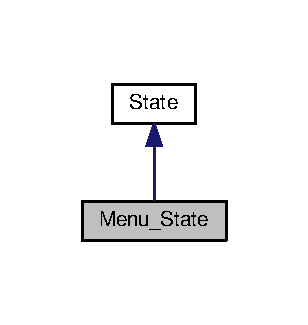
\includegraphics[width=148pt]{classMenu__State__inherit__graph}
\end{center}
\end{figure}


Collaboration diagram for Menu\+\_\+\+State\+:\nopagebreak
\begin{figure}[H]
\begin{center}
\leavevmode
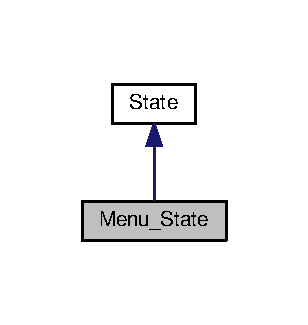
\includegraphics[width=148pt]{classMenu__State__coll__graph}
\end{center}
\end{figure}
\subsection*{Public Member Functions}
\begin{DoxyCompactItemize}
\item 
\hypertarget{classMenu__State_abcb7829ec9a970e44efa5c235e988cfb}{\hyperlink{classMenu__State_abcb7829ec9a970e44efa5c235e988cfb}{Menu\+\_\+\+State} ()}\label{classMenu__State_abcb7829ec9a970e44efa5c235e988cfb}

\begin{DoxyCompactList}\small\item\em \char`\"{}\+Constructor \+: loads all textures and fonts used in the state\char`\"{} \end{DoxyCompactList}\item 
\hypertarget{classMenu__State_a654017b2f4425a4d2e2827bc35c113eb}{void \hyperlink{classMenu__State_a654017b2f4425a4d2e2827bc35c113eb}{prepare\+\_\+simulate} () override}\label{classMenu__State_a654017b2f4425a4d2e2827bc35c113eb}

\begin{DoxyCompactList}\small\item\em \char`\"{}\+Resets the state and loads a new level into it with the help
        of the Level Parser class\char`\"{} \end{DoxyCompactList}\item 
int \hyperlink{classMenu__State_a8c8cd24b56f7123085195accaa6e1a48}{simulate} () override
\begin{DoxyCompactList}\small\item\em \char`\"{}\+Simulates each object in the state and performs actions on
        the state based on the result of the simulations\char`\"{} \end{DoxyCompactList}\item 
void \hyperlink{classMenu__State_a7a65c4db5146110cb6597b69226c4f1b}{set\+\_\+view} (sf\+::\+View \&) override
\begin{DoxyCompactList}\small\item\em \char`\"{}\+Centers the view around the player\char`\"{} \end{DoxyCompactList}\end{DoxyCompactItemize}
\subsection*{Additional Inherited Members}


\subsection{Member Function Documentation}
\hypertarget{classMenu__State_a7a65c4db5146110cb6597b69226c4f1b}{\index{Menu\+\_\+\+State@{Menu\+\_\+\+State}!set\+\_\+view@{set\+\_\+view}}
\index{set\+\_\+view@{set\+\_\+view}!Menu\+\_\+\+State@{Menu\+\_\+\+State}}
\subsubsection[{set\+\_\+view}]{\setlength{\rightskip}{0pt plus 5cm}void Menu\+\_\+\+State\+::set\+\_\+view (
\begin{DoxyParamCaption}
\item[{sf\+::\+View \&}]{view}
\end{DoxyParamCaption}
)\hspace{0.3cm}{\ttfamily [override]}, {\ttfamily [virtual]}}}\label{classMenu__State_a7a65c4db5146110cb6597b69226c4f1b}


\char`\"{}\+Centers the view around the player\char`\"{} 


\begin{DoxyParams}{Parameters}
{\em view} & \char`\"{}\+View to perform action on\char`\"{} \\
\hline
\end{DoxyParams}


Implements \hyperlink{classState}{State}.

\hypertarget{classMenu__State_a8c8cd24b56f7123085195accaa6e1a48}{\index{Menu\+\_\+\+State@{Menu\+\_\+\+State}!simulate@{simulate}}
\index{simulate@{simulate}!Menu\+\_\+\+State@{Menu\+\_\+\+State}}
\subsubsection[{simulate}]{\setlength{\rightskip}{0pt plus 5cm}int Menu\+\_\+\+State\+::simulate (
\begin{DoxyParamCaption}
{}
\end{DoxyParamCaption}
)\hspace{0.3cm}{\ttfamily [override]}, {\ttfamily [virtual]}}}\label{classMenu__State_a8c8cd24b56f7123085195accaa6e1a48}


\char`\"{}\+Simulates each object in the state and performs actions on
        the state based on the result of the simulations\char`\"{} 

\begin{DoxyReturn}{Returns}
\char`\"{}\+An integer representing the next action to be taken by the Engine object\char`\"{} 
\end{DoxyReturn}


Implements \hyperlink{classState}{State}.



The documentation for this class was generated from the following files\+:\begin{DoxyCompactItemize}
\item 
states/non\+\_\+abstract/menu\+\_\+state.\+h\item 
states/non\+\_\+abstract/menu\+\_\+state.\+cc\end{DoxyCompactItemize}

\hypertarget{classMovable__Object}{\section{Movable\+\_\+\+Object Class Reference}
\label{classMovable__Object}\index{Movable\+\_\+\+Object@{Movable\+\_\+\+Object}}
}


Inheritance diagram for Movable\+\_\+\+Object\+:\nopagebreak
\begin{figure}[H]
\begin{center}
\leavevmode
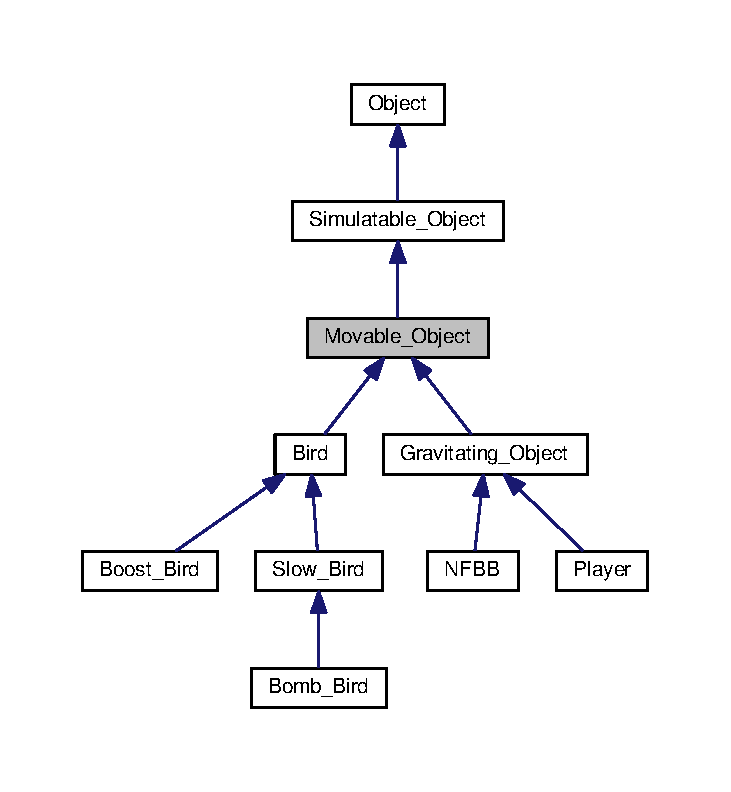
\includegraphics[width=350pt]{classMovable__Object__inherit__graph}
\end{center}
\end{figure}


Collaboration diagram for Movable\+\_\+\+Object\+:\nopagebreak
\begin{figure}[H]
\begin{center}
\leavevmode
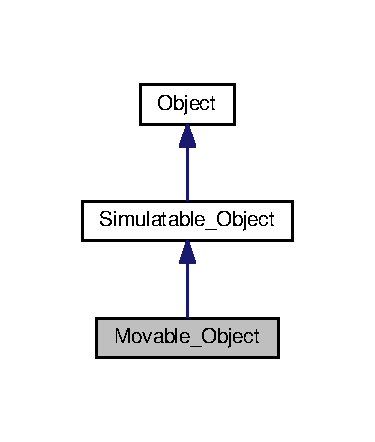
\includegraphics[width=180pt]{classMovable__Object__coll__graph}
\end{center}
\end{figure}
\subsection*{Public Member Functions}
\begin{DoxyCompactItemize}
\item 
\hyperlink{classMovable__Object_a7ef80ffc751a380e9c0beb7d4f0da9ce}{Movable\+\_\+\+Object} (const sf\+::\+Vector2f \&, const sf\+::\+Vector2f \&, const std\+::string \&, const bool=false, const sf\+::\+Texture $\ast$=nullptr)
\begin{DoxyCompactList}\small\item\em \char`\"{}\+Constructor\char`\"{} \end{DoxyCompactList}\item 
int \hyperlink{classMovable__Object_aed1d50e30dc96faea3250bee8b4af227}{prepare\+\_\+simulate} (const float)
\begin{DoxyCompactList}\small\item\em \char`\"{}\+Prepares simulation of object\char`\"{} \end{DoxyCompactList}\item 
virtual std\+::vector$<$ \hyperlink{classObject}{Object} $\ast$ $>$ \hyperlink{classMovable__Object_ac267e0c945b558b0cf533d7fbe5ee7c3}{simulate} (const int, const std\+::vector$<$ const \hyperlink{classObject}{Object} $\ast$ $>$ \&) override
\begin{DoxyCompactList}\small\item\em \char`\"{}\+Executes simulation of object\char`\"{} \end{DoxyCompactList}\item 
virtual void \hyperlink{classMovable__Object_ac9111a729082cd46a913e1877a57a930}{end\+\_\+simulate} (const std\+::vector$<$ const \hyperlink{classObject}{Object} $\ast$ $>$ \&objects) override
\begin{DoxyCompactList}\small\item\em \char`\"{}\+Executes end-\/of-\/simulation logic of object\char`\"{} \end{DoxyCompactList}\end{DoxyCompactItemize}
\subsection*{Protected Member Functions}
\begin{DoxyCompactItemize}
\item 
\hypertarget{classMovable__Object_a909989f83255795f755742be6db62713}{virtual void {\bfseries handle\+\_\+moving\+\_\+collision} (const \hyperlink{classObject}{Object} $\ast$, const sf\+::\+Vector2f \&)}\label{classMovable__Object_a909989f83255795f755742be6db62713}

\item 
\hypertarget{classMovable__Object_a7091c50aa4cd1438424737441e9ff72a}{virtual void {\bfseries collision\+\_\+state\+\_\+cleanup} ()}\label{classMovable__Object_a7091c50aa4cd1438424737441e9ff72a}

\item 
\hypertarget{classMovable__Object_a1d92a4bbc7c741bf3d1c65004eab2adb}{virtual void {\bfseries handle\+\_\+static\+\_\+collision} (const \hyperlink{classObject}{Object} $\ast$)}\label{classMovable__Object_a1d92a4bbc7c741bf3d1c65004eab2adb}

\item 
\hypertarget{classMovable__Object_a71916586f5f73c836568503dcd7b0eb7}{virtual void {\bfseries handle\+\_\+end\+\_\+collision} ()}\label{classMovable__Object_a71916586f5f73c836568503dcd7b0eb7}

\end{DoxyCompactItemize}
\subsection*{Protected Attributes}
\begin{DoxyCompactItemize}
\item 
\hypertarget{classMovable__Object_a3824126abcb82e10d65c0427ac291ef4}{sf\+::\+Vector2f {\bfseries m\+\_\+distance}}\label{classMovable__Object_a3824126abcb82e10d65c0427ac291ef4}

\item 
\hypertarget{classMovable__Object_a00d1c3d1f5cb644a9d9de84128de136f}{bool {\bfseries m\+\_\+ground\+\_\+collision} \{\}}\label{classMovable__Object_a00d1c3d1f5cb644a9d9de84128de136f}

\item 
\hypertarget{classMovable__Object_aa491f8684b9fa3d4d81047de1ad644ee}{bool {\bfseries m\+\_\+roof\+\_\+collision} \{\}}\label{classMovable__Object_aa491f8684b9fa3d4d81047de1ad644ee}

\item 
\hypertarget{classMovable__Object_aacdedf600c68dbfaa756484c39ae9229}{bool {\bfseries m\+\_\+wall\+\_\+collision} \{\}}\label{classMovable__Object_aacdedf600c68dbfaa756484c39ae9229}

\end{DoxyCompactItemize}


\subsection{Constructor \& Destructor Documentation}
\hypertarget{classMovable__Object_a7ef80ffc751a380e9c0beb7d4f0da9ce}{\index{Movable\+\_\+\+Object@{Movable\+\_\+\+Object}!Movable\+\_\+\+Object@{Movable\+\_\+\+Object}}
\index{Movable\+\_\+\+Object@{Movable\+\_\+\+Object}!Movable\+\_\+\+Object@{Movable\+\_\+\+Object}}
\subsubsection[{Movable\+\_\+\+Object}]{\setlength{\rightskip}{0pt plus 5cm}Movable\+\_\+\+Object\+::\+Movable\+\_\+\+Object (
\begin{DoxyParamCaption}
\item[{const sf\+::\+Vector2f \&}]{position, }
\item[{const sf\+::\+Vector2f \&}]{size, }
\item[{const std\+::string \&}]{type, }
\item[{const bool}]{solid = {\ttfamily false}, }
\item[{const sf\+::\+Texture $\ast$}]{texture = {\ttfamily nullptr}}
\end{DoxyParamCaption}
)}}\label{classMovable__Object_a7ef80ffc751a380e9c0beb7d4f0da9ce}


\char`\"{}\+Constructor\char`\"{} 


\begin{DoxyParams}{Parameters}
{\em position} & \char`\"{}\+Position of the object\char`\"{} \\
\hline
{\em size} & \char`\"{}\+Size of the object\char`\"{} \\
\hline
{\em type} & \char`\"{}\+Type of the object\char`\"{} \\
\hline
{\em solid} & \char`\"{}\+If the object is solid\char`\"{} \\
\hline
{\em texture} & \char`\"{}\+Texture of the object\char`\"{}" \\
\hline
\end{DoxyParams}


\subsection{Member Function Documentation}
\hypertarget{classMovable__Object_ac9111a729082cd46a913e1877a57a930}{\index{Movable\+\_\+\+Object@{Movable\+\_\+\+Object}!end\+\_\+simulate@{end\+\_\+simulate}}
\index{end\+\_\+simulate@{end\+\_\+simulate}!Movable\+\_\+\+Object@{Movable\+\_\+\+Object}}
\subsubsection[{end\+\_\+simulate}]{\setlength{\rightskip}{0pt plus 5cm}void Movable\+\_\+\+Object\+::end\+\_\+simulate (
\begin{DoxyParamCaption}
\item[{const std\+::vector$<$ const {\bf Object} $\ast$ $>$ \&}]{objects}
\end{DoxyParamCaption}
)\hspace{0.3cm}{\ttfamily [override]}, {\ttfamily [virtual]}}}\label{classMovable__Object_ac9111a729082cd46a913e1877a57a930}


\char`\"{}\+Executes end-\/of-\/simulation logic of object\char`\"{} 


\begin{DoxyParams}{Parameters}
{\em objects} & \char`\"{}\+Objects to check for collision with\char`\"{}" \\
\hline
\end{DoxyParams}


Reimplemented from \hyperlink{classSimulatable__Object_a1c542c4d9cb7ba923ea9f974e5f03e84}{Simulatable\+\_\+\+Object}.

\hypertarget{classMovable__Object_aed1d50e30dc96faea3250bee8b4af227}{\index{Movable\+\_\+\+Object@{Movable\+\_\+\+Object}!prepare\+\_\+simulate@{prepare\+\_\+simulate}}
\index{prepare\+\_\+simulate@{prepare\+\_\+simulate}!Movable\+\_\+\+Object@{Movable\+\_\+\+Object}}
\subsubsection[{prepare\+\_\+simulate}]{\setlength{\rightskip}{0pt plus 5cm}int Movable\+\_\+\+Object\+::prepare\+\_\+simulate (
\begin{DoxyParamCaption}
\item[{const float}]{distance\+\_\+modifier}
\end{DoxyParamCaption}
)}}\label{classMovable__Object_aed1d50e30dc96faea3250bee8b4af227}


\char`\"{}\+Prepares simulation of object\char`\"{} 


\begin{DoxyParams}{Parameters}
{\em distance\+\_\+modifier} & \char`\"{}\+Delta since last simulation-\/sequence\char`\"{} \\
\hline
\end{DoxyParams}
\begin{DoxyReturn}{Returns}
\char`\"{}\+Simulation cycles required by this object this simulation-\/sequence\char`\"{} 
\end{DoxyReturn}
\hypertarget{classMovable__Object_ac267e0c945b558b0cf533d7fbe5ee7c3}{\index{Movable\+\_\+\+Object@{Movable\+\_\+\+Object}!simulate@{simulate}}
\index{simulate@{simulate}!Movable\+\_\+\+Object@{Movable\+\_\+\+Object}}
\subsubsection[{simulate}]{\setlength{\rightskip}{0pt plus 5cm}std\+::vector$<$ {\bf Object} $\ast$ $>$ Movable\+\_\+\+Object\+::simulate (
\begin{DoxyParamCaption}
\item[{const int}]{simulation\+\_\+cycles, }
\item[{const std\+::vector$<$ const {\bf Object} $\ast$ $>$ \&}]{objects}
\end{DoxyParamCaption}
)\hspace{0.3cm}{\ttfamily [override]}, {\ttfamily [virtual]}}}\label{classMovable__Object_ac267e0c945b558b0cf533d7fbe5ee7c3}


\char`\"{}\+Executes simulation of object\char`\"{} 


\begin{DoxyParams}{Parameters}
{\em simulation\+\_\+cycles} & \char`\"{}\+Number simulation\+\_\+cycles the object will be subjected this simulation-\/sequence\char`\"{} \\
\hline
{\em objects} & \char`\"{}\+Objects to check for collision with\char`\"{} \\
\hline
\end{DoxyParams}
\begin{DoxyReturn}{Returns}
\char`\"{}\+New objects spawned by this object\char`\"{} 
\end{DoxyReturn}


Implements \hyperlink{classSimulatable__Object_a60fb2da770367330360a90afc7b724f1}{Simulatable\+\_\+\+Object}.



Reimplemented in \hyperlink{classBomb__Bird_a610b4c68c560a6ac30375c177642e021}{Bomb\+\_\+\+Bird}, and \hyperlink{classNFBB_a42a134a62a5d4049b74e7b4f4d7402dc}{N\+F\+B\+B}.



The documentation for this class was generated from the following files\+:\begin{DoxyCompactItemize}
\item 
objects/abstractish/movable\+\_\+object.\+h\item 
objects/abstractish/movable\+\_\+object.\+cc\end{DoxyCompactItemize}

\hypertarget{structname__null__sentry}{\section{name\+\_\+null\+\_\+sentry Struct Reference}
\label{structname__null__sentry}\index{name\+\_\+null\+\_\+sentry@{name\+\_\+null\+\_\+sentry}}
}
\subsection*{Public Member Functions}
\begin{DoxyCompactItemize}
\item 
\hypertarget{structname__null__sentry_ae5d1789457736acd9d669bc4765bd811}{{\bfseries name\+\_\+null\+\_\+sentry} (xml\+\_\+node\+\_\+struct $\ast$node\+\_\+)}\label{structname__null__sentry_ae5d1789457736acd9d669bc4765bd811}

\end{DoxyCompactItemize}
\subsection*{Public Attributes}
\begin{DoxyCompactItemize}
\item 
\hypertarget{structname__null__sentry_ab85be926948869639d135bc03324a6f0}{xml\+\_\+node\+\_\+struct $\ast$ {\bfseries node}}\label{structname__null__sentry_ab85be926948869639d135bc03324a6f0}

\item 
\hypertarget{structname__null__sentry_a8847bb799593cb873c863ab6f88299d6}{char\+\_\+t $\ast$ {\bfseries name}}\label{structname__null__sentry_a8847bb799593cb873c863ab6f88299d6}

\end{DoxyCompactItemize}


The documentation for this struct was generated from the following file\+:\begin{DoxyCompactItemize}
\item 
resources/pugixml-\/1.\+8/src/pugixml.\+cpp\end{DoxyCompactItemize}

\hypertarget{structnamespace__uri__predicate}{\section{namespace\+\_\+uri\+\_\+predicate Struct Reference}
\label{structnamespace__uri__predicate}\index{namespace\+\_\+uri\+\_\+predicate@{namespace\+\_\+uri\+\_\+predicate}}
}
\subsection*{Public Member Functions}
\begin{DoxyCompactItemize}
\item 
\hypertarget{structnamespace__uri__predicate_a25bef9c1e12b0fdc908275ae7ab7c202}{{\bfseries namespace\+\_\+uri\+\_\+predicate} (const char\+\_\+t $\ast$name)}\label{structnamespace__uri__predicate_a25bef9c1e12b0fdc908275ae7ab7c202}

\item 
\hypertarget{structnamespace__uri__predicate_a9b1508940726f332b8a6c61a1d800ade}{bool {\bfseries operator()} (xml\+\_\+attribute a) const }\label{structnamespace__uri__predicate_a9b1508940726f332b8a6c61a1d800ade}

\end{DoxyCompactItemize}
\subsection*{Public Attributes}
\begin{DoxyCompactItemize}
\item 
\hypertarget{structnamespace__uri__predicate_a80a2c051b9e57b8895c28d8fcc32e051}{const char\+\_\+t $\ast$ {\bfseries prefix}}\label{structnamespace__uri__predicate_a80a2c051b9e57b8895c28d8fcc32e051}

\item 
\hypertarget{structnamespace__uri__predicate_aa48279192e8d48b9c798f5485a2a9170}{size\+\_\+t {\bfseries prefix\+\_\+length}}\label{structnamespace__uri__predicate_aa48279192e8d48b9c798f5485a2a9170}

\end{DoxyCompactItemize}


The documentation for this struct was generated from the following file\+:\begin{DoxyCompactItemize}
\item 
resources/pugixml-\/1.\+8/src/pugixml.\+cpp\end{DoxyCompactItemize}

\hypertarget{classNFBB}{\section{N\+F\+B\+B Class Reference}
\label{classNFBB}\index{N\+F\+B\+B@{N\+F\+B\+B}}
}


Inheritance diagram for N\+F\+B\+B\+:\nopagebreak
\begin{figure}[H]
\begin{center}
\leavevmode
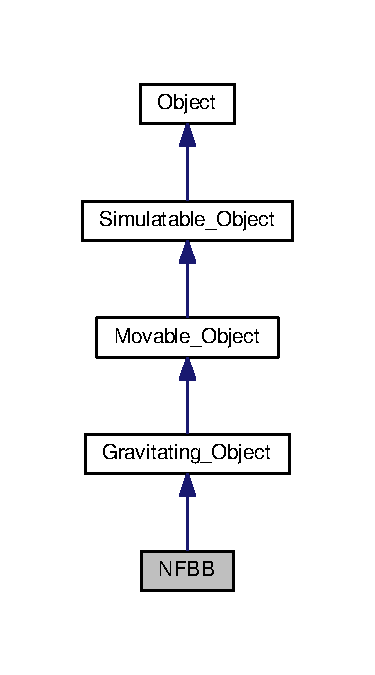
\includegraphics[width=180pt]{classNFBB__inherit__graph}
\end{center}
\end{figure}


Collaboration diagram for N\+F\+B\+B\+:\nopagebreak
\begin{figure}[H]
\begin{center}
\leavevmode
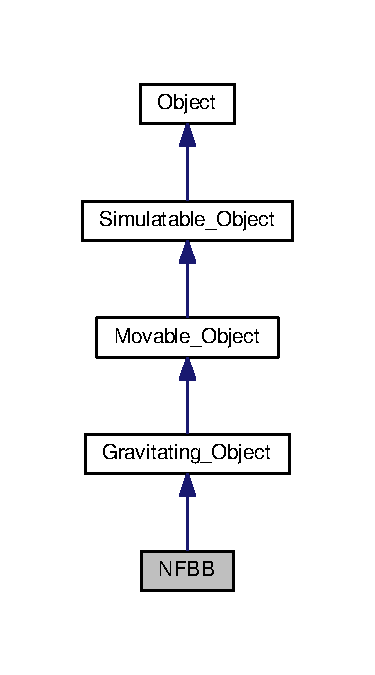
\includegraphics[width=180pt]{classNFBB__coll__graph}
\end{center}
\end{figure}
\subsection*{Public Member Functions}
\begin{DoxyCompactItemize}
\item 
\hyperlink{classNFBB_a87d7681f930eb71fd22daa8b41c8f624}{N\+F\+B\+B} (const sf\+::\+Vector2f \&, const sf\+::\+Vector2f \&, const std\+::string \&, const sf\+::\+Texture $\ast$)
\begin{DoxyCompactList}\small\item\em \char`\"{}\+Constructor\char`\"{} \end{DoxyCompactList}\item 
virtual std\+::vector$<$ \hyperlink{classObject}{Object} $\ast$ $>$ \hyperlink{classNFBB_a42a134a62a5d4049b74e7b4f4d7402dc}{simulate} (const int, const std\+::vector$<$ const \hyperlink{classObject}{Object} $\ast$ $>$ \&) overridefinal
\begin{DoxyCompactList}\small\item\em \char`\"{}\+Executes simulation of object\char`\"{} \end{DoxyCompactList}\end{DoxyCompactItemize}
\subsection*{Additional Inherited Members}


\subsection{Constructor \& Destructor Documentation}
\hypertarget{classNFBB_a87d7681f930eb71fd22daa8b41c8f624}{\index{N\+F\+B\+B@{N\+F\+B\+B}!N\+F\+B\+B@{N\+F\+B\+B}}
\index{N\+F\+B\+B@{N\+F\+B\+B}!N\+F\+B\+B@{N\+F\+B\+B}}
\subsubsection[{N\+F\+B\+B}]{\setlength{\rightskip}{0pt plus 5cm}N\+F\+B\+B\+::\+N\+F\+B\+B (
\begin{DoxyParamCaption}
\item[{const sf\+::\+Vector2f \&}]{position, }
\item[{const sf\+::\+Vector2f \&}]{size, }
\item[{const std\+::string \&}]{type, }
\item[{const sf\+::\+Texture $\ast$}]{texture}
\end{DoxyParamCaption}
)}}\label{classNFBB_a87d7681f930eb71fd22daa8b41c8f624}


\char`\"{}\+Constructor\char`\"{} 


\begin{DoxyParams}{Parameters}
{\em position} & \char`\"{}\+Position of the object\char`\"{} \\
\hline
{\em size} & \char`\"{}\+Size of the object\char`\"{} \\
\hline
{\em type} & \char`\"{}\+Type of the object\char`\"{} \\
\hline
{\em texture} & \char`\"{}\+Texture of the object\char`\"{} \\
\hline
\end{DoxyParams}


\subsection{Member Function Documentation}
\hypertarget{classNFBB_a42a134a62a5d4049b74e7b4f4d7402dc}{\index{N\+F\+B\+B@{N\+F\+B\+B}!simulate@{simulate}}
\index{simulate@{simulate}!N\+F\+B\+B@{N\+F\+B\+B}}
\subsubsection[{simulate}]{\setlength{\rightskip}{0pt plus 5cm}std\+::vector$<$ {\bf Object} $\ast$ $>$ N\+F\+B\+B\+::simulate (
\begin{DoxyParamCaption}
\item[{const int}]{simulation\+\_\+cycles, }
\item[{const std\+::vector$<$ const {\bf Object} $\ast$ $>$ \&}]{objects}
\end{DoxyParamCaption}
)\hspace{0.3cm}{\ttfamily [final]}, {\ttfamily [override]}, {\ttfamily [virtual]}}}\label{classNFBB_a42a134a62a5d4049b74e7b4f4d7402dc}


\char`\"{}\+Executes simulation of object\char`\"{} 


\begin{DoxyParams}{Parameters}
{\em simulation\+\_\+cycles} & \char`\"{}\+Number simulation\+\_\+cycles the object will be subjected this simulation-\/sequence\char`\"{} \\
\hline
{\em objects} & \char`\"{}\+Objects to check for collision with\char`\"{} \\
\hline
\end{DoxyParams}
\begin{DoxyReturn}{Returns}
\char`\"{}\+New objects spawned by this object\char`\"{} 
\end{DoxyReturn}


Reimplemented from \hyperlink{classMovable__Object_ac267e0c945b558b0cf533d7fbe5ee7c3}{Movable\+\_\+\+Object}.



The documentation for this class was generated from the following files\+:\begin{DoxyCompactItemize}
\item 
objects/non\+\_\+abstract/nfbb.\+h\item 
objects/non\+\_\+abstract/nfbb.\+cc\end{DoxyCompactItemize}

\hypertarget{structnot__equal__to}{\section{not\+\_\+equal\+\_\+to Struct Reference}
\label{structnot__equal__to}\index{not\+\_\+equal\+\_\+to@{not\+\_\+equal\+\_\+to}}
}
\subsection*{Public Member Functions}
\begin{DoxyCompactItemize}
\item 
\hypertarget{structnot__equal__to_acbcb7d0809378458b52e6ed1a07c1d7d}{{\footnotesize template$<$typename T $>$ }\\bool {\bfseries operator()} (const T \&lhs, const T \&rhs) const }\label{structnot__equal__to_acbcb7d0809378458b52e6ed1a07c1d7d}

\end{DoxyCompactItemize}


The documentation for this struct was generated from the following file\+:\begin{DoxyCompactItemize}
\item 
resources/pugixml-\/1.\+8/src/pugixml.\+cpp\end{DoxyCompactItemize}

\hypertarget{classObject}{\section{Object Class Reference}
\label{classObject}\index{Object@{Object}}
}


Inheritance diagram for Object\+:\nopagebreak
\begin{figure}[H]
\begin{center}
\leavevmode
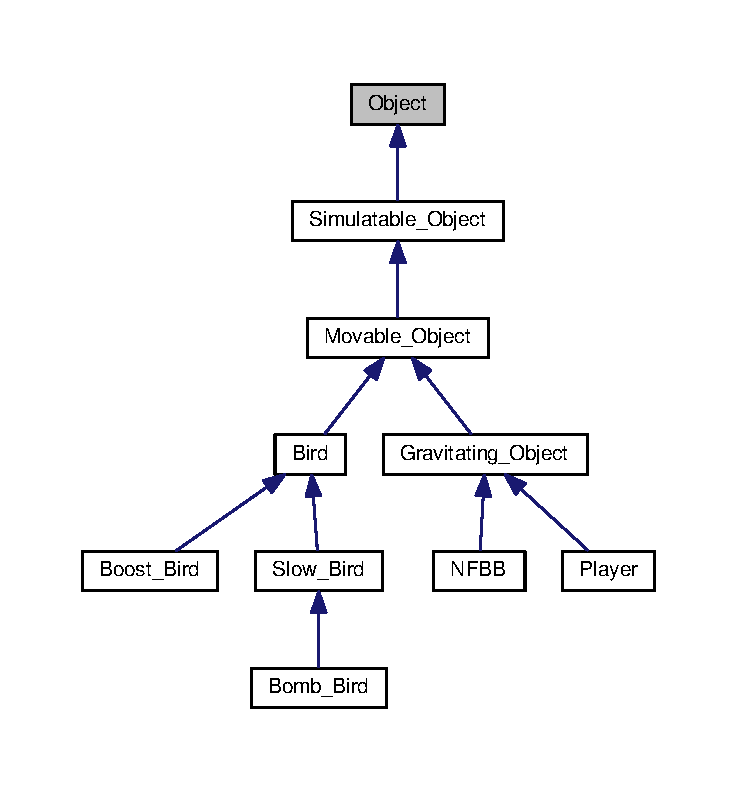
\includegraphics[width=350pt]{classObject__inherit__graph}
\end{center}
\end{figure}
\subsection*{Public Member Functions}
\begin{DoxyCompactItemize}
\item 
\hyperlink{classObject_a2df3d89d7e56659a1a0bc22d5019d587}{Object} (const sf\+::\+Vector2f \&, const sf\+::\+Vector2f \&, const std\+::string \&, const bool=false, const sf\+::\+Texture $\ast$=nullptr)
\begin{DoxyCompactList}\small\item\em \char`\"{}\+Constructor\char`\"{} \end{DoxyCompactList}\item 
\hypertarget{classObject_ad405a082a0ef9a641cd5b83ff6dd33c0}{virtual \hyperlink{classObject_ad405a082a0ef9a641cd5b83ff6dd33c0}{$\sim$\+Object} () noexcept=default}\label{classObject_ad405a082a0ef9a641cd5b83ff6dd33c0}

\begin{DoxyCompactList}\small\item\em \char`\"{}\+Virtual destrucor = default\char`\"{} \end{DoxyCompactList}\item 
std\+::string \hyperlink{classObject_a19738c1d7a0f32703a61412906edb04f}{get\+\_\+type} () const 
\item 
bool \hyperlink{classObject_ae132d029eeaaa8e3d4660951e0a35ad8}{is\+\_\+solid} () const 
\item 
bool \hyperlink{classObject_a98541d2f7380e4b5d6c805bbd7aaab01}{get\+\_\+delete\+\_\+status} () const 
\item 
sf\+::\+Rectangle\+Shape \hyperlink{classObject_a15e719bf3122cf4d8333a2b8b2f18471}{get\+\_\+shape} () const 
\begin{DoxyCompactList}\small\item\em \char`\"{}\+Returns the object's shape, which is used for drawing as well
        as getting the objects position and size\char`\"{} \end{DoxyCompactList}\end{DoxyCompactItemize}
\subsection*{Protected Attributes}
\begin{DoxyCompactItemize}
\item 
\hypertarget{classObject_a6d09f674d9c241d072a4f07934ffcac3}{const sf\+::\+Texture $\ast$ {\bfseries m\+\_\+texture}}\label{classObject_a6d09f674d9c241d072a4f07934ffcac3}

\item 
\hypertarget{classObject_a94ecef29d9e126dd4f142eb138cf93c9}{const std\+::string {\bfseries m\+\_\+type}}\label{classObject_a94ecef29d9e126dd4f142eb138cf93c9}

\item 
\hypertarget{classObject_a920a2971850ec196744477af2d7b976d}{bool {\bfseries m\+\_\+solid} \{\}}\label{classObject_a920a2971850ec196744477af2d7b976d}

\item 
\hypertarget{classObject_a122e8444050c3cc516f44be42b0aa065}{bool {\bfseries m\+\_\+delete\+\_\+status} \{\}}\label{classObject_a122e8444050c3cc516f44be42b0aa065}

\item 
\hypertarget{classObject_a4b5c1f1ad4ca0e33cdf00f74de3830f7}{sf\+::\+Rectangle\+Shape {\bfseries m\+\_\+shape}}\label{classObject_a4b5c1f1ad4ca0e33cdf00f74de3830f7}

\end{DoxyCompactItemize}


\subsection{Constructor \& Destructor Documentation}
\hypertarget{classObject_a2df3d89d7e56659a1a0bc22d5019d587}{\index{Object@{Object}!Object@{Object}}
\index{Object@{Object}!Object@{Object}}
\subsubsection[{Object}]{\setlength{\rightskip}{0pt plus 5cm}Object\+::\+Object (
\begin{DoxyParamCaption}
\item[{const sf\+::\+Vector2f \&}]{position, }
\item[{const sf\+::\+Vector2f \&}]{size, }
\item[{const std\+::string \&}]{type, }
\item[{const bool}]{solid = {\ttfamily false}, }
\item[{const sf\+::\+Texture $\ast$}]{texture = {\ttfamily nullptr}}
\end{DoxyParamCaption}
)}}\label{classObject_a2df3d89d7e56659a1a0bc22d5019d587}


\char`\"{}\+Constructor\char`\"{} 


\begin{DoxyParams}{Parameters}
{\em position} & \char`\"{}\+Position of the object\char`\"{} \\
\hline
{\em size} & \char`\"{}\+Size of the object\char`\"{} \\
\hline
{\em type} & \char`\"{}\+Type of the object\char`\"{} \\
\hline
{\em solid} & \char`\"{}\+If the object is solid\char`\"{} \\
\hline
{\em texture} & \char`\"{}\+Texture of the object\char`\"{}" \\
\hline
\end{DoxyParams}


\subsection{Member Function Documentation}
\hypertarget{classObject_a98541d2f7380e4b5d6c805bbd7aaab01}{\index{Object@{Object}!get\+\_\+delete\+\_\+status@{get\+\_\+delete\+\_\+status}}
\index{get\+\_\+delete\+\_\+status@{get\+\_\+delete\+\_\+status}!Object@{Object}}
\subsubsection[{get\+\_\+delete\+\_\+status}]{\setlength{\rightskip}{0pt plus 5cm}bool Object\+::get\+\_\+delete\+\_\+status (
\begin{DoxyParamCaption}
{}
\end{DoxyParamCaption}
) const}}\label{classObject_a98541d2f7380e4b5d6c805bbd7aaab01}
\begin{DoxyReturn}{Returns}
\char`\"{}\+If object is marked for deletion\char`\"{} 
\end{DoxyReturn}
\hypertarget{classObject_a15e719bf3122cf4d8333a2b8b2f18471}{\index{Object@{Object}!get\+\_\+shape@{get\+\_\+shape}}
\index{get\+\_\+shape@{get\+\_\+shape}!Object@{Object}}
\subsubsection[{get\+\_\+shape}]{\setlength{\rightskip}{0pt plus 5cm}sf\+::\+Rectangle\+Shape Object\+::get\+\_\+shape (
\begin{DoxyParamCaption}
{}
\end{DoxyParamCaption}
) const}}\label{classObject_a15e719bf3122cf4d8333a2b8b2f18471}


\char`\"{}\+Returns the object's shape, which is used for drawing as well
        as getting the objects position and size\char`\"{} 

\begin{DoxyReturn}{Returns}
\char`\"{}\+Shape of object\char`\"{} 
\end{DoxyReturn}
\hypertarget{classObject_a19738c1d7a0f32703a61412906edb04f}{\index{Object@{Object}!get\+\_\+type@{get\+\_\+type}}
\index{get\+\_\+type@{get\+\_\+type}!Object@{Object}}
\subsubsection[{get\+\_\+type}]{\setlength{\rightskip}{0pt plus 5cm}std\+::string Object\+::get\+\_\+type (
\begin{DoxyParamCaption}
{}
\end{DoxyParamCaption}
) const}}\label{classObject_a19738c1d7a0f32703a61412906edb04f}
\begin{DoxyReturn}{Returns}
\char`\"{}\+Type of object\char`\"{} 
\end{DoxyReturn}
\hypertarget{classObject_ae132d029eeaaa8e3d4660951e0a35ad8}{\index{Object@{Object}!is\+\_\+solid@{is\+\_\+solid}}
\index{is\+\_\+solid@{is\+\_\+solid}!Object@{Object}}
\subsubsection[{is\+\_\+solid}]{\setlength{\rightskip}{0pt plus 5cm}bool Object\+::is\+\_\+solid (
\begin{DoxyParamCaption}
{}
\end{DoxyParamCaption}
) const}}\label{classObject_ae132d029eeaaa8e3d4660951e0a35ad8}
\begin{DoxyReturn}{Returns}
\char`\"{}\+If object is solid\char`\"{} 
\end{DoxyReturn}


The documentation for this class was generated from the following files\+:\begin{DoxyCompactItemize}
\item 
objects/abstractish/object.\+h\item 
objects/abstractish/object.\+cc\end{DoxyCompactItemize}

\hypertarget{structopt__false}{\section{opt\+\_\+false Struct Reference}
\label{structopt__false}\index{opt\+\_\+false@{opt\+\_\+false}}
}
\subsection*{Public Types}
\begin{DoxyCompactItemize}
\item 
\hypertarget{structopt__false_adf1eb3ad7c3e284bd861d80d6817174f}{enum \{ {\bfseries value} = 0
 \}}\label{structopt__false_adf1eb3ad7c3e284bd861d80d6817174f}

\end{DoxyCompactItemize}


The documentation for this struct was generated from the following file\+:\begin{DoxyCompactItemize}
\item 
resources/pugixml-\/1.\+8/src/pugixml.\+cpp\end{DoxyCompactItemize}

\hypertarget{structopt__true}{\section{opt\+\_\+true Struct Reference}
\label{structopt__true}\index{opt\+\_\+true@{opt\+\_\+true}}
}
\subsection*{Public Types}
\begin{DoxyCompactItemize}
\item 
\hypertarget{structopt__true_a93a7039f202aca3a935c98aa8e069ea5}{enum \{ {\bfseries value} = 1
 \}}\label{structopt__true_a93a7039f202aca3a935c98aa8e069ea5}

\end{DoxyCompactItemize}


The documentation for this struct was generated from the following file\+:\begin{DoxyCompactItemize}
\item 
resources/pugixml-\/1.\+8/src/pugixml.\+cpp\end{DoxyCompactItemize}

\hypertarget{classPlayer}{\section{Player Class Reference}
\label{classPlayer}\index{Player@{Player}}
}


Inheritance diagram for Player\+:\nopagebreak
\begin{figure}[H]
\begin{center}
\leavevmode
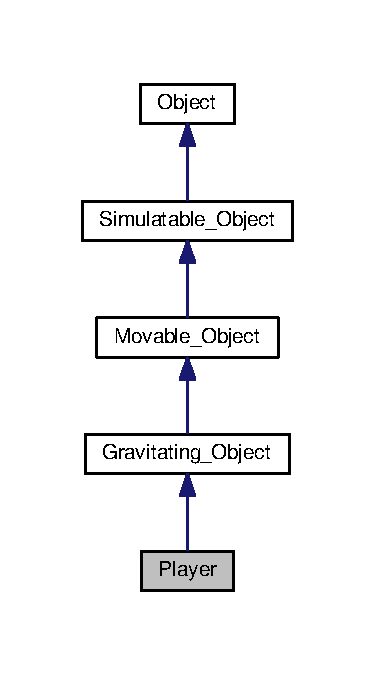
\includegraphics[width=180pt]{classPlayer__inherit__graph}
\end{center}
\end{figure}


Collaboration diagram for Player\+:\nopagebreak
\begin{figure}[H]
\begin{center}
\leavevmode
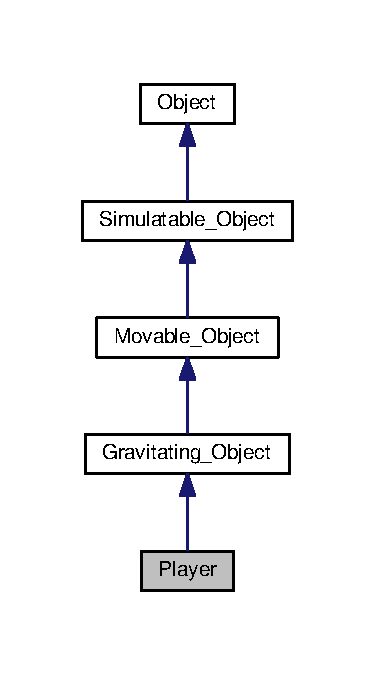
\includegraphics[width=180pt]{classPlayer__coll__graph}
\end{center}
\end{figure}
\subsection*{Public Member Functions}
\begin{DoxyCompactItemize}
\item 
\hyperlink{classPlayer_a40cd0f9599681aa40e536fc6ce47fdf2}{Player} (const sf\+::\+Vector2f \&, const sf\+::\+Vector2f \&, const std\+::string \&, const sf\+::\+Texture $\ast$, const float)
\begin{DoxyCompactList}\small\item\em \char`\"{}\+Constructor\char`\"{} \end{DoxyCompactList}\item 
virtual int \hyperlink{classPlayer_a1480bbfb767687380ad6a2bf294cdcc8}{prepare\+\_\+simulate} (const float, const float) overridefinal
\begin{DoxyCompactList}\small\item\em \char`\"{}\+Prepares simulation of object\char`\"{} \end{DoxyCompactList}\item 
const std\+::string \& \hyperlink{classPlayer_a1d89d0ff8b76784f68cf0d9e509ab242}{get\+\_\+oog\+\_\+action} () const 
\begin{DoxyCompactList}\small\item\em "Returns instructions of eventual out-\/of-\/game actions, which is used by the owning \hyperlink{classState}{State} to determine if out-\/of-\/game actions, such as quitting, should be taken" \end{DoxyCompactList}\end{DoxyCompactItemize}
\subsection*{Additional Inherited Members}


\subsection{Constructor \& Destructor Documentation}
\hypertarget{classPlayer_a40cd0f9599681aa40e536fc6ce47fdf2}{\index{Player@{Player}!Player@{Player}}
\index{Player@{Player}!Player@{Player}}
\subsubsection[{Player}]{\setlength{\rightskip}{0pt plus 5cm}Player\+::\+Player (
\begin{DoxyParamCaption}
\item[{const sf\+::\+Vector2f \&}]{position, }
\item[{const sf\+::\+Vector2f \&}]{size, }
\item[{const std\+::string \&}]{type, }
\item[{const sf\+::\+Texture $\ast$}]{texture, }
\item[{const float}]{speed}
\end{DoxyParamCaption}
)}}\label{classPlayer_a40cd0f9599681aa40e536fc6ce47fdf2}


\char`\"{}\+Constructor\char`\"{} 


\begin{DoxyParams}{Parameters}
{\em position} & \char`\"{}\+Position of the object\char`\"{} \\
\hline
{\em size} & \char`\"{}\+Size of the object\char`\"{} \\
\hline
{\em type} & \char`\"{}\+Type of the object\char`\"{} \\
\hline
{\em texture} & \char`\"{}\+Texture of the object\char`\"{} \\
\hline
{\em speed} & \char`\"{}\+Speed of the object\char`\"{} \\
\hline
\end{DoxyParams}


\subsection{Member Function Documentation}
\hypertarget{classPlayer_a1d89d0ff8b76784f68cf0d9e509ab242}{\index{Player@{Player}!get\+\_\+oog\+\_\+action@{get\+\_\+oog\+\_\+action}}
\index{get\+\_\+oog\+\_\+action@{get\+\_\+oog\+\_\+action}!Player@{Player}}
\subsubsection[{get\+\_\+oog\+\_\+action}]{\setlength{\rightskip}{0pt plus 5cm}const std\+::string \& Player\+::get\+\_\+oog\+\_\+action (
\begin{DoxyParamCaption}
{}
\end{DoxyParamCaption}
) const}}\label{classPlayer_a1d89d0ff8b76784f68cf0d9e509ab242}


"Returns instructions of eventual out-\/of-\/game actions, which is used by the owning \hyperlink{classState}{State} to determine if out-\/of-\/game actions, such as quitting, should be taken" 

\begin{DoxyReturn}{Returns}
\char`\"{}\+Return out-\/of-\/game action\char`\"{} 
\end{DoxyReturn}
\hypertarget{classPlayer_a1480bbfb767687380ad6a2bf294cdcc8}{\index{Player@{Player}!prepare\+\_\+simulate@{prepare\+\_\+simulate}}
\index{prepare\+\_\+simulate@{prepare\+\_\+simulate}!Player@{Player}}
\subsubsection[{prepare\+\_\+simulate}]{\setlength{\rightskip}{0pt plus 5cm}int Player\+::prepare\+\_\+simulate (
\begin{DoxyParamCaption}
\item[{const float}]{distance\+\_\+modifier, }
\item[{const float}]{gravity\+\_\+constant}
\end{DoxyParamCaption}
)\hspace{0.3cm}{\ttfamily [final]}, {\ttfamily [override]}, {\ttfamily [virtual]}}}\label{classPlayer_a1480bbfb767687380ad6a2bf294cdcc8}


\char`\"{}\+Prepares simulation of object\char`\"{} 


\begin{DoxyParams}{Parameters}
{\em distance\+\_\+modifier} & \char`\"{}\+Delta since last simulation-\/sequence\char`\"{} \\
\hline
{\em gravity\+\_\+constant} & \char`\"{}\+How much high the gravity is\char`\"{} \\
\hline
\end{DoxyParams}
\begin{DoxyReturn}{Returns}
\char`\"{}\+Simulation cycles required by this object this simulation-\/sequence\char`\"{} 
\end{DoxyReturn}


Reimplemented from \hyperlink{classGravitating__Object_a187404d6df6ff16a86a33a3f4a8aab85}{Gravitating\+\_\+\+Object}.



The documentation for this class was generated from the following files\+:\begin{DoxyCompactItemize}
\item 
objects/non\+\_\+abstract/player.\+h\item 
objects/non\+\_\+abstract/player.\+cc\end{DoxyCompactItemize}

\hypertarget{structboost_1_1range__const__iterator_3_01pugi_1_1xml__document_01_4}{\section{boost\+:\+:range\+\_\+const\+\_\+iterator$<$ pugi\+:\+:xml\+\_\+document $>$ Struct Template Reference}
\label{structboost_1_1range__const__iterator_3_01pugi_1_1xml__document_01_4}\index{boost\+::range\+\_\+const\+\_\+iterator$<$ pugi\+::xml\+\_\+document $>$@{boost\+::range\+\_\+const\+\_\+iterator$<$ pugi\+::xml\+\_\+document $>$}}
}
\subsection*{Public Types}
\begin{DoxyCompactItemize}
\item 
\hypertarget{structboost_1_1range__const__iterator_3_01pugi_1_1xml__document_01_4_a64a697b6f5bed6824f5ded8978018da4}{typedef \\*
\hyperlink{classpugi_1_1xml__node__iterator}{pugi\+::xml\+\_\+document\+::iterator} {\bfseries type}}\label{structboost_1_1range__const__iterator_3_01pugi_1_1xml__document_01_4_a64a697b6f5bed6824f5ded8978018da4}

\end{DoxyCompactItemize}


The documentation for this struct was generated from the following file\+:\begin{DoxyCompactItemize}
\item 
resources/pugixml-\/1.\+8/contrib/foreach.\+hpp\end{DoxyCompactItemize}

\hypertarget{structboost_1_1range__const__iterator_3_01pugi_1_1xml__node_01_4}{\section{boost\+:\+:range\+\_\+const\+\_\+iterator$<$ pugi\+:\+:xml\+\_\+node $>$ Struct Template Reference}
\label{structboost_1_1range__const__iterator_3_01pugi_1_1xml__node_01_4}\index{boost\+::range\+\_\+const\+\_\+iterator$<$ pugi\+::xml\+\_\+node $>$@{boost\+::range\+\_\+const\+\_\+iterator$<$ pugi\+::xml\+\_\+node $>$}}
}
\subsection*{Public Types}
\begin{DoxyCompactItemize}
\item 
\hypertarget{structboost_1_1range__const__iterator_3_01pugi_1_1xml__node_01_4_a15c23e25e1dc892eb0e2f6ad261c6c2d}{typedef \hyperlink{classpugi_1_1xml__node__iterator}{pugi\+::xml\+\_\+node\+::iterator} {\bfseries type}}\label{structboost_1_1range__const__iterator_3_01pugi_1_1xml__node_01_4_a15c23e25e1dc892eb0e2f6ad261c6c2d}

\end{DoxyCompactItemize}


The documentation for this struct was generated from the following file\+:\begin{DoxyCompactItemize}
\item 
resources/pugixml-\/1.\+8/contrib/foreach.\+hpp\end{DoxyCompactItemize}

\hypertarget{structboost_1_1range__mutable__iterator_3_01pugi_1_1xml__document_01_4}{\section{boost\+:\+:range\+\_\+mutable\+\_\+iterator$<$ pugi\+:\+:xml\+\_\+document $>$ Struct Template Reference}
\label{structboost_1_1range__mutable__iterator_3_01pugi_1_1xml__document_01_4}\index{boost\+::range\+\_\+mutable\+\_\+iterator$<$ pugi\+::xml\+\_\+document $>$@{boost\+::range\+\_\+mutable\+\_\+iterator$<$ pugi\+::xml\+\_\+document $>$}}
}
\subsection*{Public Types}
\begin{DoxyCompactItemize}
\item 
\hypertarget{structboost_1_1range__mutable__iterator_3_01pugi_1_1xml__document_01_4_a8523f9f4c77e5ebba00a1ae90c1d0841}{typedef \\*
\hyperlink{classpugi_1_1xml__node__iterator}{pugi\+::xml\+\_\+document\+::iterator} {\bfseries type}}\label{structboost_1_1range__mutable__iterator_3_01pugi_1_1xml__document_01_4_a8523f9f4c77e5ebba00a1ae90c1d0841}

\end{DoxyCompactItemize}


The documentation for this struct was generated from the following file\+:\begin{DoxyCompactItemize}
\item 
resources/pugixml-\/1.\+8/contrib/foreach.\+hpp\end{DoxyCompactItemize}

\hypertarget{structboost_1_1range__mutable__iterator_3_01pugi_1_1xml__node_01_4}{\section{boost\+:\+:range\+\_\+mutable\+\_\+iterator$<$ pugi\+:\+:xml\+\_\+node $>$ Struct Template Reference}
\label{structboost_1_1range__mutable__iterator_3_01pugi_1_1xml__node_01_4}\index{boost\+::range\+\_\+mutable\+\_\+iterator$<$ pugi\+::xml\+\_\+node $>$@{boost\+::range\+\_\+mutable\+\_\+iterator$<$ pugi\+::xml\+\_\+node $>$}}
}
\subsection*{Public Types}
\begin{DoxyCompactItemize}
\item 
\hypertarget{structboost_1_1range__mutable__iterator_3_01pugi_1_1xml__node_01_4_ac824e88c57d235ef4b417f87302e02af}{typedef \hyperlink{classpugi_1_1xml__node__iterator}{pugi\+::xml\+\_\+node\+::iterator} {\bfseries type}}\label{structboost_1_1range__mutable__iterator_3_01pugi_1_1xml__node_01_4_ac824e88c57d235ef4b417f87302e02af}

\end{DoxyCompactItemize}


The documentation for this struct was generated from the following file\+:\begin{DoxyCompactItemize}
\item 
resources/pugixml-\/1.\+8/contrib/foreach.\+hpp\end{DoxyCompactItemize}

\hypertarget{structsimple__walker}{\section{simple\+\_\+walker Struct Reference}
\label{structsimple__walker}\index{simple\+\_\+walker@{simple\+\_\+walker}}
}


Inheritance diagram for simple\+\_\+walker\+:
\nopagebreak
\begin{figure}[H]
\begin{center}
\leavevmode
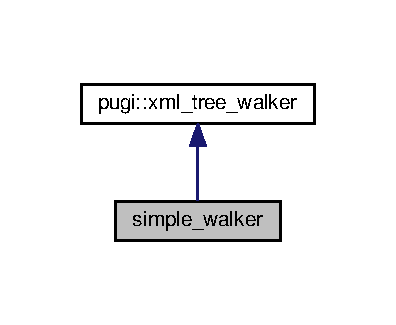
\includegraphics[width=190pt]{structsimple__walker__inherit__graph}
\end{center}
\end{figure}


Collaboration diagram for simple\+\_\+walker\+:
\nopagebreak
\begin{figure}[H]
\begin{center}
\leavevmode
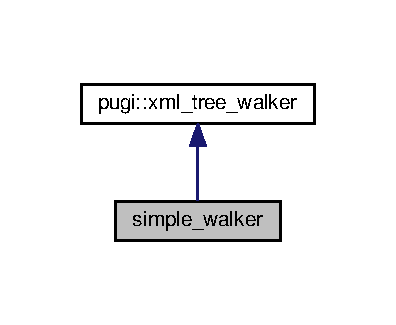
\includegraphics[width=190pt]{structsimple__walker__coll__graph}
\end{center}
\end{figure}
\subsection*{Public Member Functions}
\begin{DoxyCompactItemize}
\item 
\hypertarget{structsimple__walker_a8afb03751c939134462d557f2a3ff023}{virtual bool {\bfseries for\+\_\+each} (\hyperlink{classpugi_1_1xml__node}{pugi\+::xml\+\_\+node} \&node)}\label{structsimple__walker_a8afb03751c939134462d557f2a3ff023}

\end{DoxyCompactItemize}
\subsection*{Additional Inherited Members}


The documentation for this struct was generated from the following file\+:\begin{DoxyCompactItemize}
\item 
resources/pugixml-\/1.\+8/docs/samples/traverse\+\_\+walker.\+cpp\end{DoxyCompactItemize}

\hypertarget{classSimulatable__Object}{\section{Simulatable\+\_\+\+Object Class Reference}
\label{classSimulatable__Object}\index{Simulatable\+\_\+\+Object@{Simulatable\+\_\+\+Object}}
}


Inheritance diagram for Simulatable\+\_\+\+Object\+:\nopagebreak
\begin{figure}[H]
\begin{center}
\leavevmode
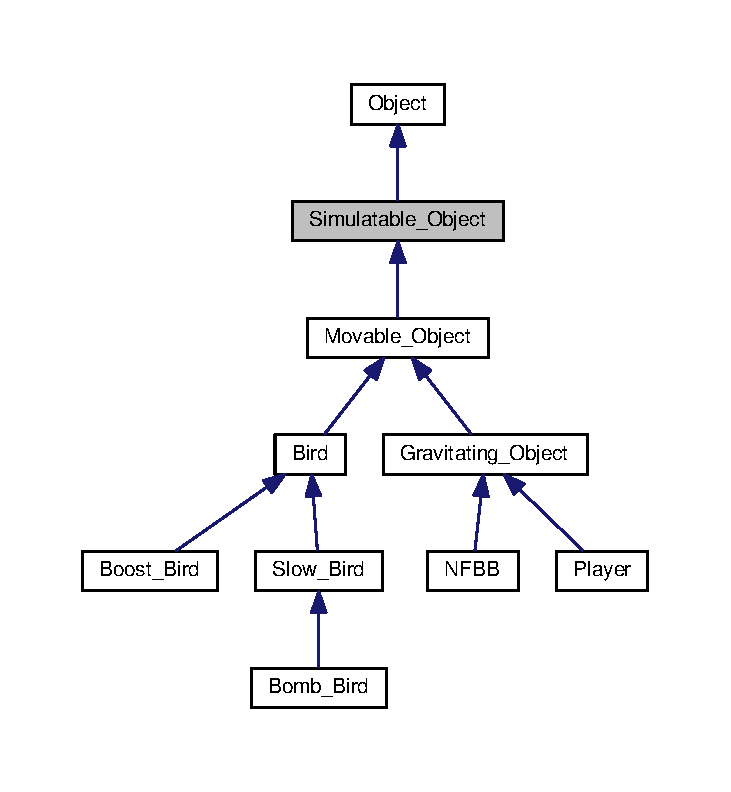
\includegraphics[width=350pt]{classSimulatable__Object__inherit__graph}
\end{center}
\end{figure}


Collaboration diagram for Simulatable\+\_\+\+Object\+:\nopagebreak
\begin{figure}[H]
\begin{center}
\leavevmode
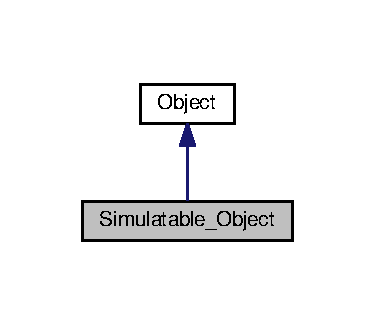
\includegraphics[width=180pt]{classSimulatable__Object__coll__graph}
\end{center}
\end{figure}
\subsection*{Public Member Functions}
\begin{DoxyCompactItemize}
\item 
\hyperlink{classSimulatable__Object_a0ca1611db5809ac78440a862ba986af7}{Simulatable\+\_\+\+Object} (const sf\+::\+Vector2f \&, const sf\+::\+Vector2f \&, const std\+::string \&, const bool=false, const sf\+::\+Texture $\ast$=nullptr)
\begin{DoxyCompactList}\small\item\em \char`\"{}\+Constructor\char`\"{} \end{DoxyCompactList}\item 
virtual int \hyperlink{classSimulatable__Object_abe7c02fe250ef5be42011890d8a7b37b}{prepare\+\_\+simulate} (const float, const float)=0
\begin{DoxyCompactList}\small\item\em \char`\"{}\+Prepares simulation of object\char`\"{} \end{DoxyCompactList}\item 
virtual std\+::vector$<$ \hyperlink{classObject}{Object} $\ast$ $>$ \hyperlink{classSimulatable__Object_a60fb2da770367330360a90afc7b724f1}{simulate} (const int, const std\+::vector$<$ const \hyperlink{classObject}{Object} $\ast$ $>$ \&)=0
\begin{DoxyCompactList}\small\item\em \char`\"{}\+Executes simulation of object\char`\"{} \end{DoxyCompactList}\item 
virtual void \hyperlink{classSimulatable__Object_a1c542c4d9cb7ba923ea9f974e5f03e84}{end\+\_\+simulate} (const std\+::vector$<$ const \hyperlink{classObject}{Object} $\ast$ $>$ \&objects)
\begin{DoxyCompactList}\small\item\em \char`\"{}\+Executes end-\/of-\/simulation logic of object\char`\"{} \end{DoxyCompactList}\end{DoxyCompactItemize}
\subsection*{Protected Member Functions}
\begin{DoxyCompactItemize}
\item 
\hypertarget{classSimulatable__Object_a2d7252861e8dea6b3bb9909421b88766}{virtual const std\+::vector\\*
$<$ const \hyperlink{classObject}{Object} $\ast$ $>$ {\bfseries get\+\_\+colliding\+\_\+objects} (const std\+::vector$<$ const \hyperlink{classObject}{Object} $\ast$ $>$ \&) const }\label{classSimulatable__Object_a2d7252861e8dea6b3bb9909421b88766}

\end{DoxyCompactItemize}
\subsection*{Additional Inherited Members}


\subsection{Constructor \& Destructor Documentation}
\hypertarget{classSimulatable__Object_a0ca1611db5809ac78440a862ba986af7}{\index{Simulatable\+\_\+\+Object@{Simulatable\+\_\+\+Object}!Simulatable\+\_\+\+Object@{Simulatable\+\_\+\+Object}}
\index{Simulatable\+\_\+\+Object@{Simulatable\+\_\+\+Object}!Simulatable\+\_\+\+Object@{Simulatable\+\_\+\+Object}}
\subsubsection[{Simulatable\+\_\+\+Object}]{\setlength{\rightskip}{0pt plus 5cm}Simulatable\+\_\+\+Object\+::\+Simulatable\+\_\+\+Object (
\begin{DoxyParamCaption}
\item[{const sf\+::\+Vector2f \&}]{position, }
\item[{const sf\+::\+Vector2f \&}]{size, }
\item[{const std\+::string \&}]{type, }
\item[{const bool}]{solid = {\ttfamily false}, }
\item[{const sf\+::\+Texture $\ast$}]{texture = {\ttfamily nullptr}}
\end{DoxyParamCaption}
)}}\label{classSimulatable__Object_a0ca1611db5809ac78440a862ba986af7}


\char`\"{}\+Constructor\char`\"{} 


\begin{DoxyParams}{Parameters}
{\em position} & \char`\"{}\+Position of the object\char`\"{} \\
\hline
{\em size} & \char`\"{}\+Size of the object\char`\"{} \\
\hline
{\em type} & \char`\"{}\+Type of the object\char`\"{} \\
\hline
{\em solid} & \char`\"{}\+If the object is solid\char`\"{} \\
\hline
{\em texture} & \char`\"{}\+Texture of the object\char`\"{}" \\
\hline
\end{DoxyParams}


\subsection{Member Function Documentation}
\hypertarget{classSimulatable__Object_a1c542c4d9cb7ba923ea9f974e5f03e84}{\index{Simulatable\+\_\+\+Object@{Simulatable\+\_\+\+Object}!end\+\_\+simulate@{end\+\_\+simulate}}
\index{end\+\_\+simulate@{end\+\_\+simulate}!Simulatable\+\_\+\+Object@{Simulatable\+\_\+\+Object}}
\subsubsection[{end\+\_\+simulate}]{\setlength{\rightskip}{0pt plus 5cm}virtual void Simulatable\+\_\+\+Object\+::end\+\_\+simulate (
\begin{DoxyParamCaption}
\item[{const std\+::vector$<$ const {\bf Object} $\ast$ $>$ \&}]{objects}
\end{DoxyParamCaption}
)\hspace{0.3cm}{\ttfamily [inline]}, {\ttfamily [virtual]}}}\label{classSimulatable__Object_a1c542c4d9cb7ba923ea9f974e5f03e84}


\char`\"{}\+Executes end-\/of-\/simulation logic of object\char`\"{} 


\begin{DoxyParams}{Parameters}
{\em objects} & \char`\"{}\+Objects to check for collision with\char`\"{}" \\
\hline
\end{DoxyParams}


Reimplemented in \hyperlink{classMovable__Object_ac9111a729082cd46a913e1877a57a930}{Movable\+\_\+\+Object}.

\hypertarget{classSimulatable__Object_abe7c02fe250ef5be42011890d8a7b37b}{\index{Simulatable\+\_\+\+Object@{Simulatable\+\_\+\+Object}!prepare\+\_\+simulate@{prepare\+\_\+simulate}}
\index{prepare\+\_\+simulate@{prepare\+\_\+simulate}!Simulatable\+\_\+\+Object@{Simulatable\+\_\+\+Object}}
\subsubsection[{prepare\+\_\+simulate}]{\setlength{\rightskip}{0pt plus 5cm}virtual int Simulatable\+\_\+\+Object\+::prepare\+\_\+simulate (
\begin{DoxyParamCaption}
\item[{const float}]{, }
\item[{const float}]{}
\end{DoxyParamCaption}
)\hspace{0.3cm}{\ttfamily [pure virtual]}}}\label{classSimulatable__Object_abe7c02fe250ef5be42011890d8a7b37b}


\char`\"{}\+Prepares simulation of object\char`\"{} 


\begin{DoxyParams}{Parameters}
{\em distance\+\_\+modifier} & \char`\"{}\+Delta since last simulation-\/sequence\char`\"{} \\
\hline
\end{DoxyParams}
\begin{DoxyReturn}{Returns}
\char`\"{}\+Simulation cycles required by this object this simulation-\/sequence\char`\"{} 
\end{DoxyReturn}


Implemented in \hyperlink{classBird_af2882ba302f03c5bdf5950cc21a39f66}{Bird}, \hyperlink{classPlayer_a1480bbfb767687380ad6a2bf294cdcc8}{Player}, and \hyperlink{classGravitating__Object_a187404d6df6ff16a86a33a3f4a8aab85}{Gravitating\+\_\+\+Object}.

\hypertarget{classSimulatable__Object_a60fb2da770367330360a90afc7b724f1}{\index{Simulatable\+\_\+\+Object@{Simulatable\+\_\+\+Object}!simulate@{simulate}}
\index{simulate@{simulate}!Simulatable\+\_\+\+Object@{Simulatable\+\_\+\+Object}}
\subsubsection[{simulate}]{\setlength{\rightskip}{0pt plus 5cm}virtual std\+::vector$<${\bf Object}$\ast$$>$ Simulatable\+\_\+\+Object\+::simulate (
\begin{DoxyParamCaption}
\item[{const int}]{, }
\item[{const std\+::vector$<$ const {\bf Object} $\ast$ $>$ \&}]{}
\end{DoxyParamCaption}
)\hspace{0.3cm}{\ttfamily [pure virtual]}}}\label{classSimulatable__Object_a60fb2da770367330360a90afc7b724f1}


\char`\"{}\+Executes simulation of object\char`\"{} 


\begin{DoxyParams}{Parameters}
{\em simulation\+\_\+cycles} & \char`\"{}\+Number simulation\+\_\+cycles the object will be subjected this simulation-\/sequence\char`\"{} \\
\hline
{\em objects} & \char`\"{}\+Objects to check for collision with\char`\"{} \\
\hline
\end{DoxyParams}
\begin{DoxyReturn}{Returns}
\char`\"{}\+New objects spawned by this object\char`\"{} 
\end{DoxyReturn}


Implemented in \hyperlink{classMovable__Object_ac267e0c945b558b0cf533d7fbe5ee7c3}{Movable\+\_\+\+Object}, \hyperlink{classBomb__Bird_a610b4c68c560a6ac30375c177642e021}{Bomb\+\_\+\+Bird}, and \hyperlink{classNFBB_a42a134a62a5d4049b74e7b4f4d7402dc}{N\+F\+B\+B}.



The documentation for this class was generated from the following files\+:\begin{DoxyCompactItemize}
\item 
objects/abstractish/simulatable\+\_\+object.\+h\item 
objects/abstractish/simulatable\+\_\+object.\+cc\end{DoxyCompactItemize}

\hypertarget{classSlow__Bird}{\section{Slow\+\_\+\+Bird Class Reference}
\label{classSlow__Bird}\index{Slow\+\_\+\+Bird@{Slow\+\_\+\+Bird}}
}


Inheritance diagram for Slow\+\_\+\+Bird\+:\nopagebreak
\begin{figure}[H]
\begin{center}
\leavevmode
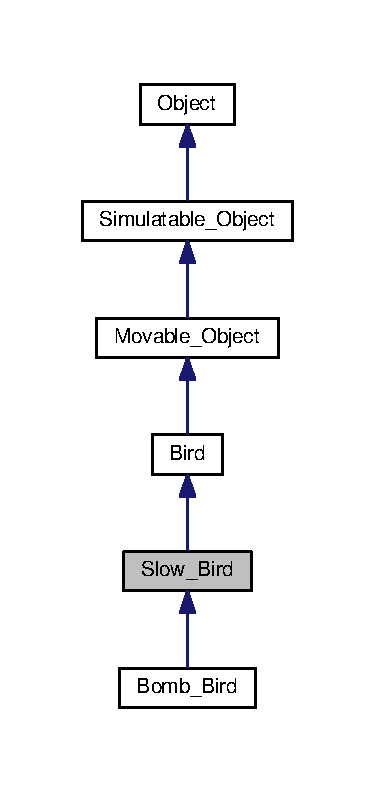
\includegraphics[width=180pt]{classSlow__Bird__inherit__graph}
\end{center}
\end{figure}


Collaboration diagram for Slow\+\_\+\+Bird\+:\nopagebreak
\begin{figure}[H]
\begin{center}
\leavevmode
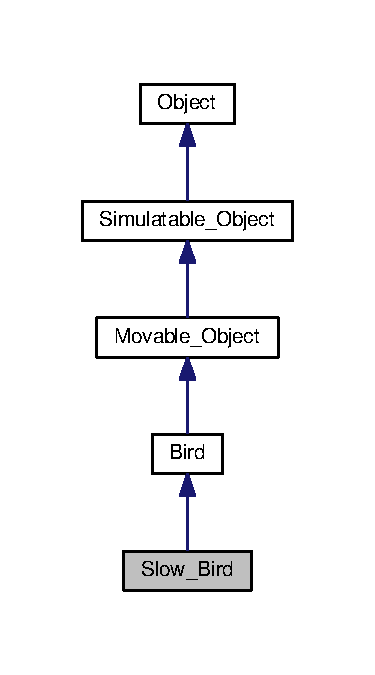
\includegraphics[width=180pt]{classSlow__Bird__coll__graph}
\end{center}
\end{figure}
\subsection*{Public Member Functions}
\begin{DoxyCompactItemize}
\item 
\hyperlink{classSlow__Bird_a52df2736474b4fe540181a43231a3f8c}{Slow\+\_\+\+Bird} (const sf\+::\+Vector2f \&, const sf\+::\+Vector2f \&, const std\+::string \&, const sf\+::\+Texture $\ast$, const float, const int)
\begin{DoxyCompactList}\small\item\em \char`\"{}\+Constructor\char`\"{} \end{DoxyCompactList}\end{DoxyCompactItemize}
\subsection*{Additional Inherited Members}


\subsection{Constructor \& Destructor Documentation}
\hypertarget{classSlow__Bird_a52df2736474b4fe540181a43231a3f8c}{\index{Slow\+\_\+\+Bird@{Slow\+\_\+\+Bird}!Slow\+\_\+\+Bird@{Slow\+\_\+\+Bird}}
\index{Slow\+\_\+\+Bird@{Slow\+\_\+\+Bird}!Slow\+\_\+\+Bird@{Slow\+\_\+\+Bird}}
\subsubsection[{Slow\+\_\+\+Bird}]{\setlength{\rightskip}{0pt plus 5cm}Slow\+\_\+\+Bird\+::\+Slow\+\_\+\+Bird (
\begin{DoxyParamCaption}
\item[{const sf\+::\+Vector2f \&}]{position, }
\item[{const sf\+::\+Vector2f \&}]{size, }
\item[{const std\+::string \&}]{type, }
\item[{const sf\+::\+Texture $\ast$}]{texture, }
\item[{const float}]{speed, }
\item[{const int}]{direction}
\end{DoxyParamCaption}
)}}\label{classSlow__Bird_a52df2736474b4fe540181a43231a3f8c}


\char`\"{}\+Constructor\char`\"{} 


\begin{DoxyParams}{Parameters}
{\em position} & \char`\"{}\+Position of the object\char`\"{} \\
\hline
{\em size} & \char`\"{}\+Size of the object\char`\"{} \\
\hline
{\em type} & \char`\"{}\+Type of the object\char`\"{} \\
\hline
{\em texture} & \char`\"{}\+Texture of the object\char`\"{} \\
\hline
{\em speed} & \char`\"{}\+Speed of the object\char`\"{} \\
\hline
{\em direction} & \char`\"{}\+Direction of the object\char`\"{} \\
\hline
{\em nfbb\+\_\+texture} & \char`\"{}\+Texture of N\+F\+B\+B-\/objects spawned by the object\char`\"{} \\
\hline
\end{DoxyParams}


The documentation for this class was generated from the following files\+:\begin{DoxyCompactItemize}
\item 
objects/non\+\_\+abstract/slow\+\_\+bird.\+h\item 
objects/non\+\_\+abstract/slow\+\_\+bird.\+cc\end{DoxyCompactItemize}

\hypertarget{classState}{\section{State Class Reference}
\label{classState}\index{State@{State}}
}


Inheritance diagram for State\+:\nopagebreak
\begin{figure}[H]
\begin{center}
\leavevmode
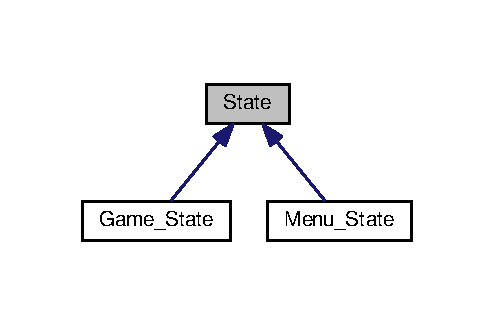
\includegraphics[width=237pt]{classState__inherit__graph}
\end{center}
\end{figure}
\subsection*{Public Member Functions}
\begin{DoxyCompactItemize}
\item 
\hypertarget{classState_a591f523d68d09675b3bd6f8e1084e642}{virtual \hyperlink{classState_a591f523d68d09675b3bd6f8e1084e642}{$\sim$\+State} () noexcept}\label{classState_a591f523d68d09675b3bd6f8e1084e642}

\begin{DoxyCompactList}\small\item\em \char`\"{}\+Virtual destructor which frees all resources owned by the state\char`\"{} \end{DoxyCompactList}\item 
\hypertarget{classState_af0cf4ef9c4b4e9a22dacf949f3df8cea}{virtual void {\bfseries prepare\+\_\+simulate} ()=0}\label{classState_af0cf4ef9c4b4e9a22dacf949f3df8cea}

\item 
\hypertarget{classState_a2fd001147b34d4a07102ba0acf680982}{virtual int {\bfseries simulate} ()=0}\label{classState_a2fd001147b34d4a07102ba0acf680982}

\item 
\hypertarget{classState_aacfda33b8dc4e6d39febdb192270a85a}{virtual void {\bfseries set\+\_\+view} (sf\+::\+View \&)=0}\label{classState_aacfda33b8dc4e6d39febdb192270a85a}

\item 
const sf\+::\+Sprite \& \hyperlink{classState_a9e132079dc08365e3c30633dd002ab8c}{get\+\_\+background} () const 
\item 
const std\+::vector$<$ const \\*
\hyperlink{classObject}{Object} $\ast$ $>$ \& \hyperlink{classState_aa234d5b01d5f75580825ea0e38074482}{get\+\_\+texturated\+\_\+objects} () const 
\item 
std\+::unordered\+\_\+map\\*
$<$ std\+::string, sf\+::\+Text $>$ \& \hyperlink{classState_a38fe48726722d318d346608f4f947121}{ref\+\_\+text\+\_\+objects} ()
\end{DoxyCompactItemize}
\subsection*{Protected Member Functions}
\begin{DoxyCompactItemize}
\item 
\hypertarget{classState_a2ebdd6e26d78ad2d34a8bf14ddb7ccf3}{virtual void \hyperlink{classState_a2ebdd6e26d78ad2d34a8bf14ddb7ccf3}{soft\+\_\+reset} ()}\label{classState_a2ebdd6e26d78ad2d34a8bf14ddb7ccf3}

\begin{DoxyCompactList}\small\item\em \char`\"{}\+Resetar statet, kan skrivas över av ärvande klasser\char`\"{} \end{DoxyCompactList}\end{DoxyCompactItemize}
\subsection*{Protected Attributes}
\begin{DoxyCompactItemize}
\item 
\hypertarget{classState_a9fe3983efbf800d94bde79b304fa0769}{std\+::unordered\+\_\+map\\*
$<$ std\+::string, sf\+::\+Texture $\ast$ $>$ {\bfseries textures}}\label{classState_a9fe3983efbf800d94bde79b304fa0769}

\item 
\hypertarget{classState_a4982a5b77746daf5e042359b45cb9a3a}{sf\+::\+Texture {\bfseries background\+\_\+texture}}\label{classState_a4982a5b77746daf5e042359b45cb9a3a}

\item 
\hypertarget{classState_addd1389225a80440a320adbb386cfe12}{sf\+::\+Sprite {\bfseries background}}\label{classState_addd1389225a80440a320adbb386cfe12}

\item 
\hypertarget{classState_ac01e57d52a3bf0d9b24c02daecd79e30}{sf\+::\+Font {\bfseries font}}\label{classState_ac01e57d52a3bf0d9b24c02daecd79e30}

\item 
\hypertarget{classState_a9f93fadc63056740b57f2b8655327fcd}{std\+::vector$<$ const \hyperlink{classObject}{Object} $\ast$ $>$ {\bfseries objects}}\label{classState_a9f93fadc63056740b57f2b8655327fcd}

\item 
\hypertarget{classState_a8f0f08cc8fcc900e4864f42d53a4d6b5}{std\+::vector$<$ const \hyperlink{classObject}{Object} $\ast$ $>$ {\bfseries texturated\+\_\+objects}}\label{classState_a8f0f08cc8fcc900e4864f42d53a4d6b5}

\item 
\hypertarget{classState_affee9f7ca66bb6a54f882b297939abbb}{std\+::unordered\+\_\+map\\*
$<$ std\+::string, sf\+::\+Text $>$ {\bfseries text\+\_\+objects}}\label{classState_affee9f7ca66bb6a54f882b297939abbb}

\end{DoxyCompactItemize}


\subsection{Member Function Documentation}
\hypertarget{classState_a9e132079dc08365e3c30633dd002ab8c}{\index{State@{State}!get\+\_\+background@{get\+\_\+background}}
\index{get\+\_\+background@{get\+\_\+background}!State@{State}}
\subsubsection[{get\+\_\+background}]{\setlength{\rightskip}{0pt plus 5cm}const sf\+::\+Sprite \& State\+::get\+\_\+background (
\begin{DoxyParamCaption}
{}
\end{DoxyParamCaption}
) const}}\label{classState_a9e132079dc08365e3c30633dd002ab8c}
\begin{DoxyReturn}{Returns}
\char`\"{}\+Returns the background set in the state\char`\"{} 
\end{DoxyReturn}
\hypertarget{classState_aa234d5b01d5f75580825ea0e38074482}{\index{State@{State}!get\+\_\+texturated\+\_\+objects@{get\+\_\+texturated\+\_\+objects}}
\index{get\+\_\+texturated\+\_\+objects@{get\+\_\+texturated\+\_\+objects}!State@{State}}
\subsubsection[{get\+\_\+texturated\+\_\+objects}]{\setlength{\rightskip}{0pt plus 5cm}const std\+::vector$<$ const {\bf Object} $\ast$ $>$ \& State\+::get\+\_\+texturated\+\_\+objects (
\begin{DoxyParamCaption}
{}
\end{DoxyParamCaption}
) const}}\label{classState_aa234d5b01d5f75580825ea0e38074482}
\begin{DoxyReturn}{Returns}
\char`\"{}\+Returns the texturated\+\_\+objects owned by the state\char`\"{} 
\end{DoxyReturn}
\hypertarget{classState_a38fe48726722d318d346608f4f947121}{\index{State@{State}!ref\+\_\+text\+\_\+objects@{ref\+\_\+text\+\_\+objects}}
\index{ref\+\_\+text\+\_\+objects@{ref\+\_\+text\+\_\+objects}!State@{State}}
\subsubsection[{ref\+\_\+text\+\_\+objects}]{\setlength{\rightskip}{0pt plus 5cm}std\+::unordered\+\_\+map$<$ std\+::string, sf\+::\+Text $>$ \& State\+::ref\+\_\+text\+\_\+objects (
\begin{DoxyParamCaption}
{}
\end{DoxyParamCaption}
)}}\label{classState_a38fe48726722d318d346608f4f947121}
\begin{DoxyReturn}{Returns}
\char`\"{}\+Returns the text\+\_\+objects owned by the state as a non-\/const reference\char`\"{} 
\end{DoxyReturn}


The documentation for this class was generated from the following files\+:\begin{DoxyCompactItemize}
\item 
states/abstract/state.\+h\item 
states/abstract/state.\+cc\end{DoxyCompactItemize}

\hypertarget{structstrconv__attribute__impl}{\section{strconv\+\_\+attribute\+\_\+impl$<$ opt\+\_\+escape $>$ Struct Template Reference}
\label{structstrconv__attribute__impl}\index{strconv\+\_\+attribute\+\_\+impl$<$ opt\+\_\+escape $>$@{strconv\+\_\+attribute\+\_\+impl$<$ opt\+\_\+escape $>$}}
}
\subsection*{Static Public Member Functions}
\begin{DoxyCompactItemize}
\item 
\hypertarget{structstrconv__attribute__impl_a9b7f8b1e860c5d022dbd29f9a89e9e27}{static char\+\_\+t $\ast$ {\bfseries parse\+\_\+wnorm} (char\+\_\+t $\ast$s, char\+\_\+t end\+\_\+quote)}\label{structstrconv__attribute__impl_a9b7f8b1e860c5d022dbd29f9a89e9e27}

\item 
\hypertarget{structstrconv__attribute__impl_a2d39998b79896af7c53c5f3dc22a526b}{static char\+\_\+t $\ast$ {\bfseries parse\+\_\+wconv} (char\+\_\+t $\ast$s, char\+\_\+t end\+\_\+quote)}\label{structstrconv__attribute__impl_a2d39998b79896af7c53c5f3dc22a526b}

\item 
\hypertarget{structstrconv__attribute__impl_a0f57ee9d69b9d626765f4a9c8af6df2e}{static char\+\_\+t $\ast$ {\bfseries parse\+\_\+eol} (char\+\_\+t $\ast$s, char\+\_\+t end\+\_\+quote)}\label{structstrconv__attribute__impl_a0f57ee9d69b9d626765f4a9c8af6df2e}

\item 
\hypertarget{structstrconv__attribute__impl_a8358dc980178e55c8669b9dcd04872d7}{static char\+\_\+t $\ast$ {\bfseries parse\+\_\+simple} (char\+\_\+t $\ast$s, char\+\_\+t end\+\_\+quote)}\label{structstrconv__attribute__impl_a8358dc980178e55c8669b9dcd04872d7}

\end{DoxyCompactItemize}


The documentation for this struct was generated from the following file\+:\begin{DoxyCompactItemize}
\item 
resources/pugixml-\/1.\+8/src/pugixml.\+cpp\end{DoxyCompactItemize}

\hypertarget{structstrconv__pcdata__impl}{\section{strconv\+\_\+pcdata\+\_\+impl$<$ opt\+\_\+trim, opt\+\_\+eol, opt\+\_\+escape $>$ Struct Template Reference}
\label{structstrconv__pcdata__impl}\index{strconv\+\_\+pcdata\+\_\+impl$<$ opt\+\_\+trim, opt\+\_\+eol, opt\+\_\+escape $>$@{strconv\+\_\+pcdata\+\_\+impl$<$ opt\+\_\+trim, opt\+\_\+eol, opt\+\_\+escape $>$}}
}
\subsection*{Static Public Member Functions}
\begin{DoxyCompactItemize}
\item 
\hypertarget{structstrconv__pcdata__impl_a0bd2c80c1df06c93d77332a4bb63b5b8}{static char\+\_\+t $\ast$ {\bfseries parse} (char\+\_\+t $\ast$s)}\label{structstrconv__pcdata__impl_a0bd2c80c1df06c93d77332a4bb63b5b8}

\end{DoxyCompactItemize}


The documentation for this struct was generated from the following file\+:\begin{DoxyCompactItemize}
\item 
resources/pugixml-\/1.\+8/src/pugixml.\+cpp\end{DoxyCompactItemize}

\hypertarget{structutf16__counter}{\section{utf16\+\_\+counter Struct Reference}
\label{structutf16__counter}\index{utf16\+\_\+counter@{utf16\+\_\+counter}}
}
\subsection*{Public Types}
\begin{DoxyCompactItemize}
\item 
\hypertarget{structutf16__counter_a0d63f9ca809d182b2f184ef93bd11107}{typedef size\+\_\+t {\bfseries value\+\_\+type}}\label{structutf16__counter_a0d63f9ca809d182b2f184ef93bd11107}

\end{DoxyCompactItemize}
\subsection*{Static Public Member Functions}
\begin{DoxyCompactItemize}
\item 
\hypertarget{structutf16__counter_a4571f3d0fbf0ce763904ec3321dcb41e}{static value\+\_\+type {\bfseries low} (value\+\_\+type result, uint32\+\_\+t)}\label{structutf16__counter_a4571f3d0fbf0ce763904ec3321dcb41e}

\item 
\hypertarget{structutf16__counter_ac1a8793996e57dc28fd22f3165628e4d}{static value\+\_\+type {\bfseries high} (value\+\_\+type result, uint32\+\_\+t)}\label{structutf16__counter_ac1a8793996e57dc28fd22f3165628e4d}

\end{DoxyCompactItemize}


The documentation for this struct was generated from the following file\+:\begin{DoxyCompactItemize}
\item 
resources/pugixml-\/1.\+8/src/pugixml.\+cpp\end{DoxyCompactItemize}

\hypertarget{structutf16__decoder}{\section{utf16\+\_\+decoder$<$ opt\+\_\+swap $>$ Struct Template Reference}
\label{structutf16__decoder}\index{utf16\+\_\+decoder$<$ opt\+\_\+swap $>$@{utf16\+\_\+decoder$<$ opt\+\_\+swap $>$}}
}
\subsection*{Public Types}
\begin{DoxyCompactItemize}
\item 
\hypertarget{structutf16__decoder_a6464d996125f65a0fc84d5fa5f11b878}{typedef uint16\+\_\+t {\bfseries type}}\label{structutf16__decoder_a6464d996125f65a0fc84d5fa5f11b878}

\end{DoxyCompactItemize}
\subsection*{Static Public Member Functions}
\begin{DoxyCompactItemize}
\item 
\hypertarget{structutf16__decoder_a76791119a94c0105611212b8ee1ea86d}{{\footnotesize template$<$typename Traits $>$ }\\static Traits\+::value\+\_\+type {\bfseries process} (const uint16\+\_\+t $\ast$data, size\+\_\+t size, typename Traits\+::value\+\_\+type result, Traits)}\label{structutf16__decoder_a76791119a94c0105611212b8ee1ea86d}

\end{DoxyCompactItemize}


The documentation for this struct was generated from the following file\+:\begin{DoxyCompactItemize}
\item 
resources/pugixml-\/1.\+8/src/pugixml.\+cpp\end{DoxyCompactItemize}

\hypertarget{structutf16__writer}{\section{utf16\+\_\+writer Struct Reference}
\label{structutf16__writer}\index{utf16\+\_\+writer@{utf16\+\_\+writer}}
}
\subsection*{Public Types}
\begin{DoxyCompactItemize}
\item 
\hypertarget{structutf16__writer_a527b705eaf5099167b8bc42423ce918c}{typedef uint16\+\_\+t $\ast$ {\bfseries value\+\_\+type}}\label{structutf16__writer_a527b705eaf5099167b8bc42423ce918c}

\end{DoxyCompactItemize}
\subsection*{Static Public Member Functions}
\begin{DoxyCompactItemize}
\item 
\hypertarget{structutf16__writer_ab11fef721a8b38de5e315d2e75d12956}{static value\+\_\+type {\bfseries low} (value\+\_\+type result, uint32\+\_\+t ch)}\label{structutf16__writer_ab11fef721a8b38de5e315d2e75d12956}

\item 
\hypertarget{structutf16__writer_a01b6ce1a567dea11daead3ca83f42d5c}{static value\+\_\+type {\bfseries high} (value\+\_\+type result, uint32\+\_\+t ch)}\label{structutf16__writer_a01b6ce1a567dea11daead3ca83f42d5c}

\item 
\hypertarget{structutf16__writer_ac14e06db126fbbef4be7efdb80fbdf4a}{static value\+\_\+type {\bfseries any} (value\+\_\+type result, uint32\+\_\+t ch)}\label{structutf16__writer_ac14e06db126fbbef4be7efdb80fbdf4a}

\end{DoxyCompactItemize}


The documentation for this struct was generated from the following file\+:\begin{DoxyCompactItemize}
\item 
resources/pugixml-\/1.\+8/src/pugixml.\+cpp\end{DoxyCompactItemize}

\hypertarget{structutf32__counter}{\section{utf32\+\_\+counter Struct Reference}
\label{structutf32__counter}\index{utf32\+\_\+counter@{utf32\+\_\+counter}}
}
\subsection*{Public Types}
\begin{DoxyCompactItemize}
\item 
\hypertarget{structutf32__counter_a6fb6728fe1a009958000f0e934fa6500}{typedef size\+\_\+t {\bfseries value\+\_\+type}}\label{structutf32__counter_a6fb6728fe1a009958000f0e934fa6500}

\end{DoxyCompactItemize}
\subsection*{Static Public Member Functions}
\begin{DoxyCompactItemize}
\item 
\hypertarget{structutf32__counter_a3a75f4840e0391ed972ddba621d49480}{static value\+\_\+type {\bfseries low} (value\+\_\+type result, uint32\+\_\+t)}\label{structutf32__counter_a3a75f4840e0391ed972ddba621d49480}

\item 
\hypertarget{structutf32__counter_aa72f5248b1dc5937330ab049bf449251}{static value\+\_\+type {\bfseries high} (value\+\_\+type result, uint32\+\_\+t)}\label{structutf32__counter_aa72f5248b1dc5937330ab049bf449251}

\end{DoxyCompactItemize}


The documentation for this struct was generated from the following file\+:\begin{DoxyCompactItemize}
\item 
resources/pugixml-\/1.\+8/src/pugixml.\+cpp\end{DoxyCompactItemize}

\hypertarget{structutf32__decoder}{\section{utf32\+\_\+decoder$<$ opt\+\_\+swap $>$ Struct Template Reference}
\label{structutf32__decoder}\index{utf32\+\_\+decoder$<$ opt\+\_\+swap $>$@{utf32\+\_\+decoder$<$ opt\+\_\+swap $>$}}
}
\subsection*{Public Types}
\begin{DoxyCompactItemize}
\item 
\hypertarget{structutf32__decoder_a817a1ba432d377e183ece6d448b7418d}{typedef uint32\+\_\+t {\bfseries type}}\label{structutf32__decoder_a817a1ba432d377e183ece6d448b7418d}

\end{DoxyCompactItemize}
\subsection*{Static Public Member Functions}
\begin{DoxyCompactItemize}
\item 
\hypertarget{structutf32__decoder_ac23eaccb8e66b323c3509b0c2307bc3f}{{\footnotesize template$<$typename Traits $>$ }\\static Traits\+::value\+\_\+type {\bfseries process} (const uint32\+\_\+t $\ast$data, size\+\_\+t size, typename Traits\+::value\+\_\+type result, Traits)}\label{structutf32__decoder_ac23eaccb8e66b323c3509b0c2307bc3f}

\end{DoxyCompactItemize}


The documentation for this struct was generated from the following file\+:\begin{DoxyCompactItemize}
\item 
resources/pugixml-\/1.\+8/src/pugixml.\+cpp\end{DoxyCompactItemize}

\hypertarget{structutf32__writer}{\section{utf32\+\_\+writer Struct Reference}
\label{structutf32__writer}\index{utf32\+\_\+writer@{utf32\+\_\+writer}}
}
\subsection*{Public Types}
\begin{DoxyCompactItemize}
\item 
\hypertarget{structutf32__writer_a2284e1fa3406f113f151ded2aaa8d4ae}{typedef uint32\+\_\+t $\ast$ {\bfseries value\+\_\+type}}\label{structutf32__writer_a2284e1fa3406f113f151ded2aaa8d4ae}

\end{DoxyCompactItemize}
\subsection*{Static Public Member Functions}
\begin{DoxyCompactItemize}
\item 
\hypertarget{structutf32__writer_a06e1b65906f7355ea54a622248095bc7}{static value\+\_\+type {\bfseries low} (value\+\_\+type result, uint32\+\_\+t ch)}\label{structutf32__writer_a06e1b65906f7355ea54a622248095bc7}

\item 
\hypertarget{structutf32__writer_a3f86d996cde3ed7cab5c31930b67c9f1}{static value\+\_\+type {\bfseries high} (value\+\_\+type result, uint32\+\_\+t ch)}\label{structutf32__writer_a3f86d996cde3ed7cab5c31930b67c9f1}

\item 
\hypertarget{structutf32__writer_aa94aaa4a13e755942e7da70ea7700d3e}{static value\+\_\+type {\bfseries any} (value\+\_\+type result, uint32\+\_\+t ch)}\label{structutf32__writer_aa94aaa4a13e755942e7da70ea7700d3e}

\end{DoxyCompactItemize}


The documentation for this struct was generated from the following file\+:\begin{DoxyCompactItemize}
\item 
resources/pugixml-\/1.\+8/src/pugixml.\+cpp\end{DoxyCompactItemize}

\hypertarget{structutf8__counter}{\section{utf8\+\_\+counter Struct Reference}
\label{structutf8__counter}\index{utf8\+\_\+counter@{utf8\+\_\+counter}}
}
\subsection*{Public Types}
\begin{DoxyCompactItemize}
\item 
\hypertarget{structutf8__counter_adb65152c007965c42184614da9c4af1b}{typedef size\+\_\+t {\bfseries value\+\_\+type}}\label{structutf8__counter_adb65152c007965c42184614da9c4af1b}

\end{DoxyCompactItemize}
\subsection*{Static Public Member Functions}
\begin{DoxyCompactItemize}
\item 
\hypertarget{structutf8__counter_a0950643189089175ae0eac9b4193534d}{static value\+\_\+type {\bfseries low} (value\+\_\+type result, uint32\+\_\+t ch)}\label{structutf8__counter_a0950643189089175ae0eac9b4193534d}

\item 
\hypertarget{structutf8__counter_ab16e675980a15e1ede2e4cd18d19f7b1}{static value\+\_\+type {\bfseries high} (value\+\_\+type result, uint32\+\_\+t)}\label{structutf8__counter_ab16e675980a15e1ede2e4cd18d19f7b1}

\end{DoxyCompactItemize}


The documentation for this struct was generated from the following file\+:\begin{DoxyCompactItemize}
\item 
resources/pugixml-\/1.\+8/src/pugixml.\+cpp\end{DoxyCompactItemize}

\hypertarget{structutf8__decoder}{\section{utf8\+\_\+decoder Struct Reference}
\label{structutf8__decoder}\index{utf8\+\_\+decoder@{utf8\+\_\+decoder}}
}
\subsection*{Public Types}
\begin{DoxyCompactItemize}
\item 
\hypertarget{structutf8__decoder_a83f88a84f37817f5f4aeb32a3c07b1c2}{typedef uint8\+\_\+t {\bfseries type}}\label{structutf8__decoder_a83f88a84f37817f5f4aeb32a3c07b1c2}

\end{DoxyCompactItemize}
\subsection*{Static Public Member Functions}
\begin{DoxyCompactItemize}
\item 
\hypertarget{structutf8__decoder_a542f1dede169ee2078d2f616ea03c158}{{\footnotesize template$<$typename Traits $>$ }\\static Traits\+::value\+\_\+type {\bfseries process} (const uint8\+\_\+t $\ast$data, size\+\_\+t size, typename Traits\+::value\+\_\+type result, Traits)}\label{structutf8__decoder_a542f1dede169ee2078d2f616ea03c158}

\end{DoxyCompactItemize}


The documentation for this struct was generated from the following file\+:\begin{DoxyCompactItemize}
\item 
resources/pugixml-\/1.\+8/src/pugixml.\+cpp\end{DoxyCompactItemize}

\hypertarget{structutf8__writer}{\section{utf8\+\_\+writer Struct Reference}
\label{structutf8__writer}\index{utf8\+\_\+writer@{utf8\+\_\+writer}}
}
\subsection*{Public Types}
\begin{DoxyCompactItemize}
\item 
\hypertarget{structutf8__writer_af25ec3c651f9a4a3f193573a4e95002b}{typedef uint8\+\_\+t $\ast$ {\bfseries value\+\_\+type}}\label{structutf8__writer_af25ec3c651f9a4a3f193573a4e95002b}

\end{DoxyCompactItemize}
\subsection*{Static Public Member Functions}
\begin{DoxyCompactItemize}
\item 
\hypertarget{structutf8__writer_ac4ec52da6f37225ba4fde259bff2f86c}{static value\+\_\+type {\bfseries low} (value\+\_\+type result, uint32\+\_\+t ch)}\label{structutf8__writer_ac4ec52da6f37225ba4fde259bff2f86c}

\item 
\hypertarget{structutf8__writer_ac03dfaf797d599afdf0be7def86ff9b9}{static value\+\_\+type {\bfseries high} (value\+\_\+type result, uint32\+\_\+t ch)}\label{structutf8__writer_ac03dfaf797d599afdf0be7def86ff9b9}

\item 
\hypertarget{structutf8__writer_a288e9c5f3720b95ae6b77330ad38dd56}{static value\+\_\+type {\bfseries any} (value\+\_\+type result, uint32\+\_\+t ch)}\label{structutf8__writer_a288e9c5f3720b95ae6b77330ad38dd56}

\end{DoxyCompactItemize}


The documentation for this struct was generated from the following file\+:\begin{DoxyCompactItemize}
\item 
resources/pugixml-\/1.\+8/src/pugixml.\+cpp\end{DoxyCompactItemize}

\hypertarget{structwchar__decoder}{\section{wchar\+\_\+decoder Struct Reference}
\label{structwchar__decoder}\index{wchar\+\_\+decoder@{wchar\+\_\+decoder}}
}
\subsection*{Public Types}
\begin{DoxyCompactItemize}
\item 
\hypertarget{structwchar__decoder_aafb01f17f51c610468f88b8820e36b7a}{typedef wchar\+\_\+t {\bfseries type}}\label{structwchar__decoder_aafb01f17f51c610468f88b8820e36b7a}

\end{DoxyCompactItemize}
\subsection*{Static Public Member Functions}
\begin{DoxyCompactItemize}
\item 
\hypertarget{structwchar__decoder_a965801bc1ce931281e10ee153586071c}{{\footnotesize template$<$typename Traits $>$ }\\static Traits\+::value\+\_\+type {\bfseries process} (const wchar\+\_\+t $\ast$data, size\+\_\+t size, typename Traits\+::value\+\_\+type result, Traits traits)}\label{structwchar__decoder_a965801bc1ce931281e10ee153586071c}

\end{DoxyCompactItemize}


The documentation for this struct was generated from the following file\+:\begin{DoxyCompactItemize}
\item 
resources/pugixml-\/1.\+8/src/pugixml.\+cpp\end{DoxyCompactItemize}

\hypertarget{structwchar__selector}{\section{wchar\+\_\+selector$<$ size $>$ Struct Template Reference}
\label{structwchar__selector}\index{wchar\+\_\+selector$<$ size $>$@{wchar\+\_\+selector$<$ size $>$}}
}


The documentation for this struct was generated from the following file\+:\begin{DoxyCompactItemize}
\item 
resources/pugixml-\/1.\+8/src/pugixml.\+cpp\end{DoxyCompactItemize}

\hypertarget{structwchar__selector_3_012_01_4}{\section{wchar\+\_\+selector$<$ 2 $>$ Struct Template Reference}
\label{structwchar__selector_3_012_01_4}\index{wchar\+\_\+selector$<$ 2 $>$@{wchar\+\_\+selector$<$ 2 $>$}}
}
\subsection*{Public Types}
\begin{DoxyCompactItemize}
\item 
\hypertarget{structwchar__selector_3_012_01_4_a60517f9b159ad60977ca7c3d2739c168}{typedef uint16\+\_\+t {\bfseries type}}\label{structwchar__selector_3_012_01_4_a60517f9b159ad60977ca7c3d2739c168}

\item 
\hypertarget{structwchar__selector_3_012_01_4_a108682c81b16127f3bec2501f02cb9d8}{typedef \hyperlink{structutf16__counter}{utf16\+\_\+counter} {\bfseries counter}}\label{structwchar__selector_3_012_01_4_a108682c81b16127f3bec2501f02cb9d8}

\item 
\hypertarget{structwchar__selector_3_012_01_4_af84979f9b8cd883798fe4e99820d6073}{typedef \hyperlink{structutf16__writer}{utf16\+\_\+writer} {\bfseries writer}}\label{structwchar__selector_3_012_01_4_af84979f9b8cd883798fe4e99820d6073}

\item 
\hypertarget{structwchar__selector_3_012_01_4_a74001138c16e29a1892b903b8778760b}{typedef \hyperlink{structutf16__decoder}{utf16\+\_\+decoder}$<$ \hyperlink{structopt__false}{opt\+\_\+false} $>$ {\bfseries decoder}}\label{structwchar__selector_3_012_01_4_a74001138c16e29a1892b903b8778760b}

\end{DoxyCompactItemize}


The documentation for this struct was generated from the following file\+:\begin{DoxyCompactItemize}
\item 
resources/pugixml-\/1.\+8/src/pugixml.\+cpp\end{DoxyCompactItemize}

\hypertarget{structwchar__selector_3_014_01_4}{\section{wchar\+\_\+selector$<$ 4 $>$ Struct Template Reference}
\label{structwchar__selector_3_014_01_4}\index{wchar\+\_\+selector$<$ 4 $>$@{wchar\+\_\+selector$<$ 4 $>$}}
}
\subsection*{Public Types}
\begin{DoxyCompactItemize}
\item 
\hypertarget{structwchar__selector_3_014_01_4_af45ac603ab6fefec66e5c29044b4eed6}{typedef uint32\+\_\+t {\bfseries type}}\label{structwchar__selector_3_014_01_4_af45ac603ab6fefec66e5c29044b4eed6}

\item 
\hypertarget{structwchar__selector_3_014_01_4_a7d7c585ae0819660112b8c8683971b97}{typedef \hyperlink{structutf32__counter}{utf32\+\_\+counter} {\bfseries counter}}\label{structwchar__selector_3_014_01_4_a7d7c585ae0819660112b8c8683971b97}

\item 
\hypertarget{structwchar__selector_3_014_01_4_a48042e7fe51c4661397ae7afe3905243}{typedef \hyperlink{structutf32__writer}{utf32\+\_\+writer} {\bfseries writer}}\label{structwchar__selector_3_014_01_4_a48042e7fe51c4661397ae7afe3905243}

\item 
\hypertarget{structwchar__selector_3_014_01_4_add0a8302007d5e5def40457afc32ba78}{typedef \hyperlink{structutf32__decoder}{utf32\+\_\+decoder}$<$ \hyperlink{structopt__false}{opt\+\_\+false} $>$ {\bfseries decoder}}\label{structwchar__selector_3_014_01_4_add0a8302007d5e5def40457afc32ba78}

\end{DoxyCompactItemize}


The documentation for this struct was generated from the following file\+:\begin{DoxyCompactItemize}
\item 
resources/pugixml-\/1.\+8/src/pugixml.\+cpp\end{DoxyCompactItemize}

\hypertarget{structxml__allocator}{\section{xml\+\_\+allocator Struct Reference}
\label{structxml__allocator}\index{xml\+\_\+allocator@{xml\+\_\+allocator}}
}


Inheritance diagram for xml\+\_\+allocator\+:
\nopagebreak
\begin{figure}[H]
\begin{center}
\leavevmode
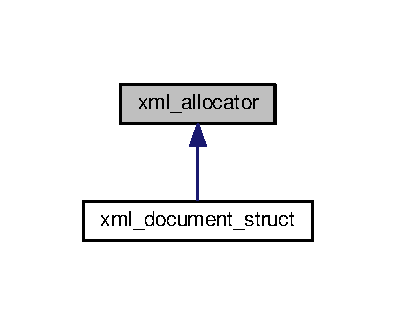
\includegraphics[width=190pt]{structxml__allocator__inherit__graph}
\end{center}
\end{figure}


Collaboration diagram for xml\+\_\+allocator\+:
\nopagebreak
\begin{figure}[H]
\begin{center}
\leavevmode
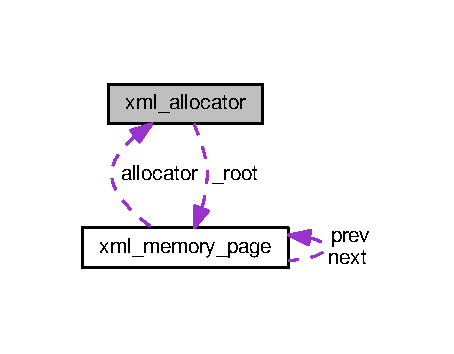
\includegraphics[width=218pt]{structxml__allocator__coll__graph}
\end{center}
\end{figure}
\subsection*{Public Member Functions}
\begin{DoxyCompactItemize}
\item 
\hypertarget{structxml__allocator_ad41b1a18595953aa71a470b45921c0fd}{{\bfseries xml\+\_\+allocator} (\hyperlink{structxml__memory__page}{xml\+\_\+memory\+\_\+page} $\ast$root)}\label{structxml__allocator_ad41b1a18595953aa71a470b45921c0fd}

\item 
\hypertarget{structxml__allocator_a4b399b01e530220ec5849b912b84063b}{\hyperlink{structxml__memory__page}{xml\+\_\+memory\+\_\+page} $\ast$ {\bfseries allocate\+\_\+page} (size\+\_\+t data\+\_\+size)}\label{structxml__allocator_a4b399b01e530220ec5849b912b84063b}

\item 
\hypertarget{structxml__allocator_a30bb557bc040de54c041c6d3dca6772e}{void $\ast$ {\bfseries allocate\+\_\+memory\+\_\+oob} (size\+\_\+t size, \hyperlink{structxml__memory__page}{xml\+\_\+memory\+\_\+page} $\ast$\&out\+\_\+page)}\label{structxml__allocator_a30bb557bc040de54c041c6d3dca6772e}

\item 
\hypertarget{structxml__allocator_afac0b9fac2c2962972f60d0346eb4f39}{void $\ast$ {\bfseries allocate\+\_\+memory} (size\+\_\+t size, \hyperlink{structxml__memory__page}{xml\+\_\+memory\+\_\+page} $\ast$\&out\+\_\+page)}\label{structxml__allocator_afac0b9fac2c2962972f60d0346eb4f39}

\item 
\hypertarget{structxml__allocator_a5c7a0614c72c3e73f561bb3f98c314e0}{void $\ast$ {\bfseries allocate\+\_\+object} (size\+\_\+t size, \hyperlink{structxml__memory__page}{xml\+\_\+memory\+\_\+page} $\ast$\&out\+\_\+page)}\label{structxml__allocator_a5c7a0614c72c3e73f561bb3f98c314e0}

\item 
\hypertarget{structxml__allocator_a5df417155487cce4e0460b123ac33dc6}{void {\bfseries deallocate\+\_\+memory} (void $\ast$ptr, size\+\_\+t size, \hyperlink{structxml__memory__page}{xml\+\_\+memory\+\_\+page} $\ast$page)}\label{structxml__allocator_a5df417155487cce4e0460b123ac33dc6}

\item 
\hypertarget{structxml__allocator_ac5ec2b5d41672d6494a2742e95e525b3}{char\+\_\+t $\ast$ {\bfseries allocate\+\_\+string} (size\+\_\+t length)}\label{structxml__allocator_ac5ec2b5d41672d6494a2742e95e525b3}

\item 
\hypertarget{structxml__allocator_af32c538db4d562c2d0bfe15f7c0aa879}{void {\bfseries deallocate\+\_\+string} (char\+\_\+t $\ast$string)}\label{structxml__allocator_af32c538db4d562c2d0bfe15f7c0aa879}

\item 
\hypertarget{structxml__allocator_ac831a283ec3bcbe22fd3ce3be98ec347}{bool {\bfseries reserve} ()}\label{structxml__allocator_ac831a283ec3bcbe22fd3ce3be98ec347}

\end{DoxyCompactItemize}
\subsection*{Static Public Member Functions}
\begin{DoxyCompactItemize}
\item 
\hypertarget{structxml__allocator_a1c6bfe15a257a094f55659f8d71c209e}{static void {\bfseries deallocate\+\_\+page} (\hyperlink{structxml__memory__page}{xml\+\_\+memory\+\_\+page} $\ast$page)}\label{structxml__allocator_a1c6bfe15a257a094f55659f8d71c209e}

\end{DoxyCompactItemize}
\subsection*{Public Attributes}
\begin{DoxyCompactItemize}
\item 
\hypertarget{structxml__allocator_a38082e85b23743620a257f997a00bb69}{\hyperlink{structxml__memory__page}{xml\+\_\+memory\+\_\+page} $\ast$ {\bfseries \+\_\+root}}\label{structxml__allocator_a38082e85b23743620a257f997a00bb69}

\item 
\hypertarget{structxml__allocator_a4908b4aaa8cbbc3bf936ab8a938053c0}{size\+\_\+t {\bfseries \+\_\+busy\+\_\+size}}\label{structxml__allocator_a4908b4aaa8cbbc3bf936ab8a938053c0}

\end{DoxyCompactItemize}


The documentation for this struct was generated from the following file\+:\begin{DoxyCompactItemize}
\item 
resources/pugixml-\/1.\+8/src/pugixml.\+cpp\end{DoxyCompactItemize}

\hypertarget{classpugi_1_1xml__attribute}{\section{pugi\+:\+:xml\+\_\+attribute Class Reference}
\label{classpugi_1_1xml__attribute}\index{pugi\+::xml\+\_\+attribute@{pugi\+::xml\+\_\+attribute}}
}
\subsection*{Public Member Functions}
\begin{DoxyCompactItemize}
\item 
\hypertarget{classpugi_1_1xml__attribute_a32b0c063842c2073445cd8c89f1c0db2}{{\bfseries xml\+\_\+attribute} (\hyperlink{structpugi_1_1xml__attribute__struct}{xml\+\_\+attribute\+\_\+struct} $\ast$attr)}\label{classpugi_1_1xml__attribute_a32b0c063842c2073445cd8c89f1c0db2}

\item 
\hypertarget{classpugi_1_1xml__attribute_a108510c1375f1317b7ddb7d4bc15b707}{{\bfseries operator unspecified\+\_\+bool\+\_\+type} () const }\label{classpugi_1_1xml__attribute_a108510c1375f1317b7ddb7d4bc15b707}

\item 
\hypertarget{classpugi_1_1xml__attribute_a0425c1b376c41d71f71416db9b1e1e6b}{bool {\bfseries operator!} () const }\label{classpugi_1_1xml__attribute_a0425c1b376c41d71f71416db9b1e1e6b}

\item 
\hypertarget{classpugi_1_1xml__attribute_ac1ab6dfce7d2a7aa0a6a24c7b84f0a5e}{bool {\bfseries operator==} (const \hyperlink{classpugi_1_1xml__attribute}{xml\+\_\+attribute} \&r) const }\label{classpugi_1_1xml__attribute_ac1ab6dfce7d2a7aa0a6a24c7b84f0a5e}

\item 
\hypertarget{classpugi_1_1xml__attribute_a76b57111453b0873b0065fe3c2fe386d}{bool {\bfseries operator!=} (const \hyperlink{classpugi_1_1xml__attribute}{xml\+\_\+attribute} \&r) const }\label{classpugi_1_1xml__attribute_a76b57111453b0873b0065fe3c2fe386d}

\item 
\hypertarget{classpugi_1_1xml__attribute_ab887d475d793b4740e53e69b9f908af6}{bool {\bfseries operator$<$} (const \hyperlink{classpugi_1_1xml__attribute}{xml\+\_\+attribute} \&r) const }\label{classpugi_1_1xml__attribute_ab887d475d793b4740e53e69b9f908af6}

\item 
\hypertarget{classpugi_1_1xml__attribute_a11ab6168bb3df31dd23956cc5bd0b871}{bool {\bfseries operator$>$} (const \hyperlink{classpugi_1_1xml__attribute}{xml\+\_\+attribute} \&r) const }\label{classpugi_1_1xml__attribute_a11ab6168bb3df31dd23956cc5bd0b871}

\item 
\hypertarget{classpugi_1_1xml__attribute_ae45e069db2452f535c349c5a605c90e6}{bool {\bfseries operator$<$=} (const \hyperlink{classpugi_1_1xml__attribute}{xml\+\_\+attribute} \&r) const }\label{classpugi_1_1xml__attribute_ae45e069db2452f535c349c5a605c90e6}

\item 
\hypertarget{classpugi_1_1xml__attribute_afaff39714d8bd51f537f372d299d68cd}{bool {\bfseries operator$>$=} (const \hyperlink{classpugi_1_1xml__attribute}{xml\+\_\+attribute} \&r) const }\label{classpugi_1_1xml__attribute_afaff39714d8bd51f537f372d299d68cd}

\item 
\hypertarget{classpugi_1_1xml__attribute_a961a571d7397e1803c3f63cf96052c53}{bool {\bfseries empty} () const }\label{classpugi_1_1xml__attribute_a961a571d7397e1803c3f63cf96052c53}

\item 
\hypertarget{classpugi_1_1xml__attribute_a98377c82f36c74f211d16db275577334}{const char\+\_\+t $\ast$ {\bfseries name} () const }\label{classpugi_1_1xml__attribute_a98377c82f36c74f211d16db275577334}

\item 
\hypertarget{classpugi_1_1xml__attribute_ad535b73777f3eaa1c0c0a3c168683bd3}{const char\+\_\+t $\ast$ {\bfseries value} () const }\label{classpugi_1_1xml__attribute_ad535b73777f3eaa1c0c0a3c168683bd3}

\item 
\hypertarget{classpugi_1_1xml__attribute_a583f470d768f5f8a4df0ebb2e016a88d}{const char\+\_\+t $\ast$ {\bfseries as\+\_\+string} (const char\+\_\+t $\ast$def=P\+U\+G\+I\+X\+M\+L\+\_\+\+T\+E\+X\+T(\char`\"{}\char`\"{})) const }\label{classpugi_1_1xml__attribute_a583f470d768f5f8a4df0ebb2e016a88d}

\item 
\hypertarget{classpugi_1_1xml__attribute_afe009e964b9cec96c77495ef1ae6d91f}{int {\bfseries as\+\_\+int} (int def=0) const }\label{classpugi_1_1xml__attribute_afe009e964b9cec96c77495ef1ae6d91f}

\item 
\hypertarget{classpugi_1_1xml__attribute_af89be4951cf7567053bcbb66ce013156}{unsigned int {\bfseries as\+\_\+uint} (unsigned int def=0) const }\label{classpugi_1_1xml__attribute_af89be4951cf7567053bcbb66ce013156}

\item 
\hypertarget{classpugi_1_1xml__attribute_acd8d510ac7825b0f52f4795d2cc5e00b}{double {\bfseries as\+\_\+double} (double def=0) const }\label{classpugi_1_1xml__attribute_acd8d510ac7825b0f52f4795d2cc5e00b}

\item 
\hypertarget{classpugi_1_1xml__attribute_a23f960683dba03f32ed4da19a10c769d}{float {\bfseries as\+\_\+float} (float def=0) const }\label{classpugi_1_1xml__attribute_a23f960683dba03f32ed4da19a10c769d}

\item 
\hypertarget{classpugi_1_1xml__attribute_a715646ddcfcd9f327934f9083f949796}{bool {\bfseries as\+\_\+bool} (bool def=false) const }\label{classpugi_1_1xml__attribute_a715646ddcfcd9f327934f9083f949796}

\item 
\hypertarget{classpugi_1_1xml__attribute_ae8ffb5ef48338f27015337a6f57b6595}{bool {\bfseries set\+\_\+name} (const char\+\_\+t $\ast$rhs)}\label{classpugi_1_1xml__attribute_ae8ffb5ef48338f27015337a6f57b6595}

\item 
\hypertarget{classpugi_1_1xml__attribute_af2ca1f0d13ee8f661bc17524bedc13d7}{bool {\bfseries set\+\_\+value} (const char\+\_\+t $\ast$rhs)}\label{classpugi_1_1xml__attribute_af2ca1f0d13ee8f661bc17524bedc13d7}

\item 
\hypertarget{classpugi_1_1xml__attribute_aa9fcffccebda6ae6169e4d17265bd39a}{bool {\bfseries set\+\_\+value} (int rhs)}\label{classpugi_1_1xml__attribute_aa9fcffccebda6ae6169e4d17265bd39a}

\item 
\hypertarget{classpugi_1_1xml__attribute_abffdc566e5e2805c493f18f8424f5024}{bool {\bfseries set\+\_\+value} (unsigned int rhs)}\label{classpugi_1_1xml__attribute_abffdc566e5e2805c493f18f8424f5024}

\item 
\hypertarget{classpugi_1_1xml__attribute_a5286c75a0dec007f677421065ea38c0d}{bool {\bfseries set\+\_\+value} (long rhs)}\label{classpugi_1_1xml__attribute_a5286c75a0dec007f677421065ea38c0d}

\item 
\hypertarget{classpugi_1_1xml__attribute_a46482d404fe44f655aba4a8f6f44211e}{bool {\bfseries set\+\_\+value} (unsigned long rhs)}\label{classpugi_1_1xml__attribute_a46482d404fe44f655aba4a8f6f44211e}

\item 
\hypertarget{classpugi_1_1xml__attribute_a5e58f7565792ba3afd432325f824f1b3}{bool {\bfseries set\+\_\+value} (double rhs)}\label{classpugi_1_1xml__attribute_a5e58f7565792ba3afd432325f824f1b3}

\item 
\hypertarget{classpugi_1_1xml__attribute_aa400312f09d9c476f8a374aeaf403be3}{bool {\bfseries set\+\_\+value} (float rhs)}\label{classpugi_1_1xml__attribute_aa400312f09d9c476f8a374aeaf403be3}

\item 
\hypertarget{classpugi_1_1xml__attribute_a33ab85a706a18f88241081ab8b0f823f}{bool {\bfseries set\+\_\+value} (bool rhs)}\label{classpugi_1_1xml__attribute_a33ab85a706a18f88241081ab8b0f823f}

\item 
\hypertarget{classpugi_1_1xml__attribute_a957f7613ba25623fa3bdf1c50346b869}{\hyperlink{classpugi_1_1xml__attribute}{xml\+\_\+attribute} \& {\bfseries operator=} (const char\+\_\+t $\ast$rhs)}\label{classpugi_1_1xml__attribute_a957f7613ba25623fa3bdf1c50346b869}

\item 
\hypertarget{classpugi_1_1xml__attribute_a15f8f489bf3170dbadf28d4a89b20201}{\hyperlink{classpugi_1_1xml__attribute}{xml\+\_\+attribute} \& {\bfseries operator=} (int rhs)}\label{classpugi_1_1xml__attribute_a15f8f489bf3170dbadf28d4a89b20201}

\item 
\hypertarget{classpugi_1_1xml__attribute_a7f9f6b7ef7456873cc1c4957a806c958}{\hyperlink{classpugi_1_1xml__attribute}{xml\+\_\+attribute} \& {\bfseries operator=} (unsigned int rhs)}\label{classpugi_1_1xml__attribute_a7f9f6b7ef7456873cc1c4957a806c958}

\item 
\hypertarget{classpugi_1_1xml__attribute_a5509850879b2584167959cdeb2d38238}{\hyperlink{classpugi_1_1xml__attribute}{xml\+\_\+attribute} \& {\bfseries operator=} (long rhs)}\label{classpugi_1_1xml__attribute_a5509850879b2584167959cdeb2d38238}

\item 
\hypertarget{classpugi_1_1xml__attribute_a1347701ba3f5f7556b1430383b916b9f}{\hyperlink{classpugi_1_1xml__attribute}{xml\+\_\+attribute} \& {\bfseries operator=} (unsigned long rhs)}\label{classpugi_1_1xml__attribute_a1347701ba3f5f7556b1430383b916b9f}

\item 
\hypertarget{classpugi_1_1xml__attribute_a4383afaf2e420ed45c563b2b82a3661f}{\hyperlink{classpugi_1_1xml__attribute}{xml\+\_\+attribute} \& {\bfseries operator=} (double rhs)}\label{classpugi_1_1xml__attribute_a4383afaf2e420ed45c563b2b82a3661f}

\item 
\hypertarget{classpugi_1_1xml__attribute_a09c274a217b439fceecf8e9102636f92}{\hyperlink{classpugi_1_1xml__attribute}{xml\+\_\+attribute} \& {\bfseries operator=} (float rhs)}\label{classpugi_1_1xml__attribute_a09c274a217b439fceecf8e9102636f92}

\item 
\hypertarget{classpugi_1_1xml__attribute_ae23d29ab032d5ff7c875f5bbe4d6ab3c}{\hyperlink{classpugi_1_1xml__attribute}{xml\+\_\+attribute} \& {\bfseries operator=} (bool rhs)}\label{classpugi_1_1xml__attribute_ae23d29ab032d5ff7c875f5bbe4d6ab3c}

\item 
\hypertarget{classpugi_1_1xml__attribute_a71b0ee33f833781a94d6d35adfc0daac}{\hyperlink{classpugi_1_1xml__attribute}{xml\+\_\+attribute} {\bfseries next\+\_\+attribute} () const }\label{classpugi_1_1xml__attribute_a71b0ee33f833781a94d6d35adfc0daac}

\item 
\hypertarget{classpugi_1_1xml__attribute_aee4fc29d1645bddc70f1a174654b9d10}{\hyperlink{classpugi_1_1xml__attribute}{xml\+\_\+attribute} {\bfseries previous\+\_\+attribute} () const }\label{classpugi_1_1xml__attribute_aee4fc29d1645bddc70f1a174654b9d10}

\item 
\hypertarget{classpugi_1_1xml__attribute_a1c9776e159263d00082a395891d8470f}{size\+\_\+t {\bfseries hash\+\_\+value} () const }\label{classpugi_1_1xml__attribute_a1c9776e159263d00082a395891d8470f}

\item 
\hypertarget{classpugi_1_1xml__attribute_aa8543b8406bfddd2607c8dcdb54c5369}{\hyperlink{structpugi_1_1xml__attribute__struct}{xml\+\_\+attribute\+\_\+struct} $\ast$ {\bfseries internal\+\_\+object} () const }\label{classpugi_1_1xml__attribute_aa8543b8406bfddd2607c8dcdb54c5369}

\end{DoxyCompactItemize}
\subsection*{Friends}
\begin{DoxyCompactItemize}
\item 
\hypertarget{classpugi_1_1xml__attribute_aeff34dec57ee910e3344631528969539}{class {\bfseries xml\+\_\+attribute\+\_\+iterator}}\label{classpugi_1_1xml__attribute_aeff34dec57ee910e3344631528969539}

\item 
\hypertarget{classpugi_1_1xml__attribute_a156d917a92815c7b593bd5ef19f6d5fb}{class {\bfseries xml\+\_\+node}}\label{classpugi_1_1xml__attribute_a156d917a92815c7b593bd5ef19f6d5fb}

\end{DoxyCompactItemize}


The documentation for this class was generated from the following files\+:\begin{DoxyCompactItemize}
\item 
resources/pugixml-\/1.\+8/src/pugixml.\+hpp\item 
resources/pugixml-\/1.\+8/src/pugixml.\+cpp\end{DoxyCompactItemize}

\hypertarget{classpugi_1_1xml__attribute__iterator}{\section{pugi\+:\+:xml\+\_\+attribute\+\_\+iterator Class Reference}
\label{classpugi_1_1xml__attribute__iterator}\index{pugi\+::xml\+\_\+attribute\+\_\+iterator@{pugi\+::xml\+\_\+attribute\+\_\+iterator}}
}
\subsection*{Public Types}
\begin{DoxyCompactItemize}
\item 
\hypertarget{classpugi_1_1xml__attribute__iterator_a00b3eecf2aba886a673ad2319be88618}{typedef ptrdiff\+\_\+t {\bfseries difference\+\_\+type}}\label{classpugi_1_1xml__attribute__iterator_a00b3eecf2aba886a673ad2319be88618}

\item 
\hypertarget{classpugi_1_1xml__attribute__iterator_a2b0e779f12de813d7a806056ebed8907}{typedef \hyperlink{classpugi_1_1xml__attribute}{xml\+\_\+attribute} {\bfseries value\+\_\+type}}\label{classpugi_1_1xml__attribute__iterator_a2b0e779f12de813d7a806056ebed8907}

\item 
\hypertarget{classpugi_1_1xml__attribute__iterator_a6ed6fb3197abb02ffa848ad6b9b7a1be}{typedef \hyperlink{classpugi_1_1xml__attribute}{xml\+\_\+attribute} $\ast$ {\bfseries pointer}}\label{classpugi_1_1xml__attribute__iterator_a6ed6fb3197abb02ffa848ad6b9b7a1be}

\item 
\hypertarget{classpugi_1_1xml__attribute__iterator_ade97045a1217d0a7897e5f5873297117}{typedef \hyperlink{classpugi_1_1xml__attribute}{xml\+\_\+attribute} \& {\bfseries reference}}\label{classpugi_1_1xml__attribute__iterator_ade97045a1217d0a7897e5f5873297117}

\item 
\hypertarget{classpugi_1_1xml__attribute__iterator_aad988273a3e4cdc5fa3eb879dbdc8d35}{typedef \\*
std\+::bidirectional\+\_\+iterator\+\_\+tag {\bfseries iterator\+\_\+category}}\label{classpugi_1_1xml__attribute__iterator_aad988273a3e4cdc5fa3eb879dbdc8d35}

\end{DoxyCompactItemize}
\subsection*{Public Member Functions}
\begin{DoxyCompactItemize}
\item 
\hypertarget{classpugi_1_1xml__attribute__iterator_a7310bb0a37f918b7b499f9ccfc52df52}{{\bfseries xml\+\_\+attribute\+\_\+iterator} (const \hyperlink{classpugi_1_1xml__attribute}{xml\+\_\+attribute} \&attr, const \hyperlink{classpugi_1_1xml__node}{xml\+\_\+node} \&parent)}\label{classpugi_1_1xml__attribute__iterator_a7310bb0a37f918b7b499f9ccfc52df52}

\item 
\hypertarget{classpugi_1_1xml__attribute__iterator_a59277df18741e5243c83e040b03e49ed}{bool {\bfseries operator==} (const \hyperlink{classpugi_1_1xml__attribute__iterator}{xml\+\_\+attribute\+\_\+iterator} \&rhs) const }\label{classpugi_1_1xml__attribute__iterator_a59277df18741e5243c83e040b03e49ed}

\item 
\hypertarget{classpugi_1_1xml__attribute__iterator_aed17d2f060c0c792a5f93dfca0f6fb33}{bool {\bfseries operator!=} (const \hyperlink{classpugi_1_1xml__attribute__iterator}{xml\+\_\+attribute\+\_\+iterator} \&rhs) const }\label{classpugi_1_1xml__attribute__iterator_aed17d2f060c0c792a5f93dfca0f6fb33}

\item 
\hypertarget{classpugi_1_1xml__attribute__iterator_a896b6564606b6e24c46b1e10a63df47a}{\hyperlink{classpugi_1_1xml__attribute}{xml\+\_\+attribute} \& {\bfseries operator$\ast$} () const }\label{classpugi_1_1xml__attribute__iterator_a896b6564606b6e24c46b1e10a63df47a}

\item 
\hypertarget{classpugi_1_1xml__attribute__iterator_aa6b76277e8acd1a7eabe226179a006f6}{\hyperlink{classpugi_1_1xml__attribute}{xml\+\_\+attribute} $\ast$ {\bfseries operator-\/$>$} () const }\label{classpugi_1_1xml__attribute__iterator_aa6b76277e8acd1a7eabe226179a006f6}

\item 
\hypertarget{classpugi_1_1xml__attribute__iterator_af291afcde44b67e836e148af904e6f0f}{const \hyperlink{classpugi_1_1xml__attribute__iterator}{xml\+\_\+attribute\+\_\+iterator} \& {\bfseries operator++} ()}\label{classpugi_1_1xml__attribute__iterator_af291afcde44b67e836e148af904e6f0f}

\item 
\hypertarget{classpugi_1_1xml__attribute__iterator_aae744b06711aea8ebd68159cd4e0aaaa}{\hyperlink{classpugi_1_1xml__attribute__iterator}{xml\+\_\+attribute\+\_\+iterator} {\bfseries operator++} (int)}\label{classpugi_1_1xml__attribute__iterator_aae744b06711aea8ebd68159cd4e0aaaa}

\item 
\hypertarget{classpugi_1_1xml__attribute__iterator_a7ac06eb61d47a9e57bcd0fd2434c6243}{const \hyperlink{classpugi_1_1xml__attribute__iterator}{xml\+\_\+attribute\+\_\+iterator} \& {\bfseries operator-\/-\/} ()}\label{classpugi_1_1xml__attribute__iterator_a7ac06eb61d47a9e57bcd0fd2434c6243}

\item 
\hypertarget{classpugi_1_1xml__attribute__iterator_a48737f6e77abe7fa3e80841597dc93e1}{\hyperlink{classpugi_1_1xml__attribute__iterator}{xml\+\_\+attribute\+\_\+iterator} {\bfseries operator-\/-\/} (int)}\label{classpugi_1_1xml__attribute__iterator_a48737f6e77abe7fa3e80841597dc93e1}

\end{DoxyCompactItemize}
\subsection*{Friends}
\begin{DoxyCompactItemize}
\item 
\hypertarget{classpugi_1_1xml__attribute__iterator_a156d917a92815c7b593bd5ef19f6d5fb}{class {\bfseries xml\+\_\+node}}\label{classpugi_1_1xml__attribute__iterator_a156d917a92815c7b593bd5ef19f6d5fb}

\end{DoxyCompactItemize}


The documentation for this class was generated from the following files\+:\begin{DoxyCompactItemize}
\item 
resources/pugixml-\/1.\+8/src/pugixml.\+hpp\item 
resources/pugixml-\/1.\+8/src/pugixml.\+cpp\end{DoxyCompactItemize}

\hypertarget{structpugi_1_1xml__attribute__struct}{\section{pugi\+:\+:xml\+\_\+attribute\+\_\+struct Struct Reference}
\label{structpugi_1_1xml__attribute__struct}\index{pugi\+::xml\+\_\+attribute\+\_\+struct@{pugi\+::xml\+\_\+attribute\+\_\+struct}}
}


Collaboration diagram for pugi\+:\+:xml\+\_\+attribute\+\_\+struct\+:
\nopagebreak
\begin{figure}[H]
\begin{center}
\leavevmode
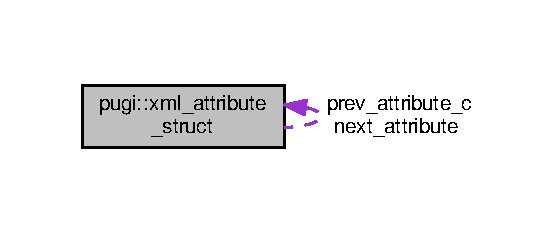
\includegraphics[width=267pt]{structpugi_1_1xml__attribute__struct__coll__graph}
\end{center}
\end{figure}
\subsection*{Public Member Functions}
\begin{DoxyCompactItemize}
\item 
\hypertarget{structpugi_1_1xml__attribute__struct_a57bb21cb72613e746a659efdd6425b94}{{\bfseries xml\+\_\+attribute\+\_\+struct} (impl\+::xml\+\_\+memory\+\_\+page $\ast$page)}\label{structpugi_1_1xml__attribute__struct_a57bb21cb72613e746a659efdd6425b94}

\end{DoxyCompactItemize}
\subsection*{Public Attributes}
\begin{DoxyCompactItemize}
\item 
\hypertarget{structpugi_1_1xml__attribute__struct_a0dca6ca6c129bbf87a7ebaf87f3e12de}{uintptr\+\_\+t {\bfseries header}}\label{structpugi_1_1xml__attribute__struct_a0dca6ca6c129bbf87a7ebaf87f3e12de}

\item 
\hypertarget{structpugi_1_1xml__attribute__struct_aa886c4aae23a132e1704717721ee2c19}{char\+\_\+t $\ast$ {\bfseries name}}\label{structpugi_1_1xml__attribute__struct_aa886c4aae23a132e1704717721ee2c19}

\item 
\hypertarget{structpugi_1_1xml__attribute__struct_ae652627d56cb9dcc0afdd1fbf6570364}{char\+\_\+t $\ast$ {\bfseries value}}\label{structpugi_1_1xml__attribute__struct_ae652627d56cb9dcc0afdd1fbf6570364}

\item 
\hypertarget{structpugi_1_1xml__attribute__struct_a0e3a022235b316e4cfc1034ceb7d7862}{\hyperlink{structpugi_1_1xml__attribute__struct}{xml\+\_\+attribute\+\_\+struct} $\ast$ {\bfseries prev\+\_\+attribute\+\_\+c}}\label{structpugi_1_1xml__attribute__struct_a0e3a022235b316e4cfc1034ceb7d7862}

\item 
\hypertarget{structpugi_1_1xml__attribute__struct_a9860c0eb7fa72dc9b69ee9b0575f9efc}{\hyperlink{structpugi_1_1xml__attribute__struct}{xml\+\_\+attribute\+\_\+struct} $\ast$ {\bfseries next\+\_\+attribute}}\label{structpugi_1_1xml__attribute__struct_a9860c0eb7fa72dc9b69ee9b0575f9efc}

\end{DoxyCompactItemize}


The documentation for this struct was generated from the following file\+:\begin{DoxyCompactItemize}
\item 
resources/pugixml-\/1.\+8/src/pugixml.\+cpp\end{DoxyCompactItemize}

\hypertarget{classxml__buffered__writer}{\section{xml\+\_\+buffered\+\_\+writer Class Reference}
\label{classxml__buffered__writer}\index{xml\+\_\+buffered\+\_\+writer@{xml\+\_\+buffered\+\_\+writer}}
}
\subsection*{Public Types}
\begin{DoxyCompactItemize}
\item 
\hypertarget{classxml__buffered__writer_a684aec07739ea6e60d47440eee97b4f6}{enum \{ {\bfseries bufcapacitybytes}, 
{\bfseries bufcapacity} = bufcapacitybytes / (sizeof(char\+\_\+t) + 4)
 \}}\label{classxml__buffered__writer_a684aec07739ea6e60d47440eee97b4f6}

\end{DoxyCompactItemize}
\subsection*{Public Member Functions}
\begin{DoxyCompactItemize}
\item 
\hypertarget{classxml__buffered__writer_a3c22ad246e2aebb6597935baf4a223a7}{{\bfseries xml\+\_\+buffered\+\_\+writer} (xml\+\_\+writer \&writer\+\_\+, xml\+\_\+encoding user\+\_\+encoding)}\label{classxml__buffered__writer_a3c22ad246e2aebb6597935baf4a223a7}

\item 
\hypertarget{classxml__buffered__writer_a4789b8661f9ff4e5e4bb4226f7d45997}{size\+\_\+t {\bfseries flush} ()}\label{classxml__buffered__writer_a4789b8661f9ff4e5e4bb4226f7d45997}

\item 
\hypertarget{classxml__buffered__writer_aa733cb2cd0d5fcacec92c67a7f26c553}{void {\bfseries flush} (const char\+\_\+t $\ast$data, size\+\_\+t size)}\label{classxml__buffered__writer_aa733cb2cd0d5fcacec92c67a7f26c553}

\item 
\hypertarget{classxml__buffered__writer_a119f9db2f60e578e69ac81177e932fb3}{void {\bfseries write\+\_\+direct} (const char\+\_\+t $\ast$data, size\+\_\+t length)}\label{classxml__buffered__writer_a119f9db2f60e578e69ac81177e932fb3}

\item 
\hypertarget{classxml__buffered__writer_ae62b84beff660555acb76e277f967c0d}{void {\bfseries write\+\_\+buffer} (const char\+\_\+t $\ast$data, size\+\_\+t length)}\label{classxml__buffered__writer_ae62b84beff660555acb76e277f967c0d}

\item 
\hypertarget{classxml__buffered__writer_a1699556c38e942f7c1db1b98ddf15642}{void {\bfseries write\+\_\+string} (const char\+\_\+t $\ast$data)}\label{classxml__buffered__writer_a1699556c38e942f7c1db1b98ddf15642}

\item 
\hypertarget{classxml__buffered__writer_a1aa829bd551a69dd9005d2d46063308f}{void {\bfseries write} (char\+\_\+t d0)}\label{classxml__buffered__writer_a1aa829bd551a69dd9005d2d46063308f}

\item 
\hypertarget{classxml__buffered__writer_a4cd6e908908e17c9b07eba34f7317791}{void {\bfseries write} (char\+\_\+t d0, char\+\_\+t d1)}\label{classxml__buffered__writer_a4cd6e908908e17c9b07eba34f7317791}

\item 
\hypertarget{classxml__buffered__writer_af82b277c1ef5c75d1901bb5a8eb4507f}{void {\bfseries write} (char\+\_\+t d0, char\+\_\+t d1, char\+\_\+t d2)}\label{classxml__buffered__writer_af82b277c1ef5c75d1901bb5a8eb4507f}

\item 
\hypertarget{classxml__buffered__writer_af679f459dfa0af257c190b8db57e7dcb}{void {\bfseries write} (char\+\_\+t d0, char\+\_\+t d1, char\+\_\+t d2, char\+\_\+t d3)}\label{classxml__buffered__writer_af679f459dfa0af257c190b8db57e7dcb}

\item 
\hypertarget{classxml__buffered__writer_aad4a4f18223ec3cb1ff607425119b85f}{void {\bfseries write} (char\+\_\+t d0, char\+\_\+t d1, char\+\_\+t d2, char\+\_\+t d3, char\+\_\+t d4)}\label{classxml__buffered__writer_aad4a4f18223ec3cb1ff607425119b85f}

\item 
\hypertarget{classxml__buffered__writer_ae6af5067d768c24b9c20422f76737f29}{void {\bfseries write} (char\+\_\+t d0, char\+\_\+t d1, char\+\_\+t d2, char\+\_\+t d3, char\+\_\+t d4, char\+\_\+t d5)}\label{classxml__buffered__writer_ae6af5067d768c24b9c20422f76737f29}

\end{DoxyCompactItemize}
\subsection*{Public Attributes}
\begin{DoxyCompactItemize}
\item 
\hypertarget{classxml__buffered__writer_a84c87765fbdf444d981ffb0f67899dd4}{char\+\_\+t {\bfseries buffer} \mbox{[}bufcapacity\mbox{]}}\label{classxml__buffered__writer_a84c87765fbdf444d981ffb0f67899dd4}

\item 
\hypertarget{classxml__buffered__writer_a74fd3d695095835afa0f7671ac33037c}{\begin{tabbing}
xx\=xx\=xx\=xx\=xx\=xx\=xx\=xx\=xx\=\kill
union \{\\
\hypertarget{unionxml__buffered__writer_1_1@3_ac672c70ba0597cf94d35c352ac563891}{\>uint8\_t {\bfseries data\_u8} \mbox{[}4 $\ast$bufcapacity\mbox{]}\\
\hypertarget{unionxml__buffered__writer_1_1@3_aa969d3724efe221a68927947e3a5196d}{\>uint16\_t {\bfseries data\_u16} \mbox{[}2 $\ast$bufcapacity\mbox{]}\\
\hypertarget{unionxml__buffered__writer_1_1@3_afa54826d8227c4ee661e1a9cc1e1acf2}{\>uint32\_t {\bfseries data\_u32} \mbox{[}bufcapacity\mbox{]}\\
\hypertarget{unionxml__buffered__writer_1_1@3_a6f21e839a1c66901995c8aae5cc9ad7b}{\>char\_t {\bfseries data\_char} \mbox{[}bufcapacity\mbox{]}\\
\} {\bfseries scratch}}\label{classxml__buffered__writer_a74fd3d695095835afa0f7671ac33037c}
\\

\end{tabbing}\item 
\hypertarget{classxml__buffered__writer_a37cdd45f867937e1978565f5a0fa318b}{xml\+\_\+writer \& {\bfseries writer}}\label{classxml__buffered__writer_a37cdd45f867937e1978565f5a0fa318b}

\item 
\hypertarget{classxml__buffered__writer_a6bad6a93035d796939d84bee30e74ce7}{size\+\_\+t {\bfseries bufsize}}\label{classxml__buffered__writer_a6bad6a93035d796939d84bee30e74ce7}

\item 
\hypertarget{classxml__buffered__writer_ab810a7286598172e1549561b285f08fb}{xml\+\_\+encoding {\bfseries encoding}}\label{classxml__buffered__writer_ab810a7286598172e1549561b285f08fb}

\end{DoxyCompactItemize}


The documentation for this class was generated from the following file\+:\begin{DoxyCompactItemize}
\item 
resources/pugixml-\/1.\+8/src/pugixml.\+cpp\end{DoxyCompactItemize}

\hypertarget{classpugi_1_1xml__document}{\section{pugi\+:\+:xml\+\_\+document Class Reference}
\label{classpugi_1_1xml__document}\index{pugi\+::xml\+\_\+document@{pugi\+::xml\+\_\+document}}
}


Inheritance diagram for pugi\+:\+:xml\+\_\+document\+:
\nopagebreak
\begin{figure}[H]
\begin{center}
\leavevmode
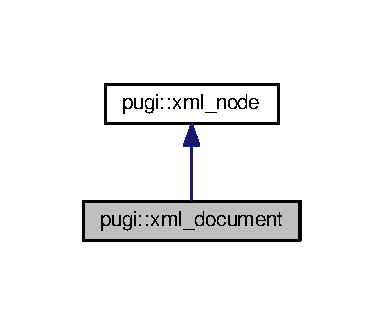
\includegraphics[width=184pt]{classpugi_1_1xml__document__inherit__graph}
\end{center}
\end{figure}


Collaboration diagram for pugi\+:\+:xml\+\_\+document\+:
\nopagebreak
\begin{figure}[H]
\begin{center}
\leavevmode
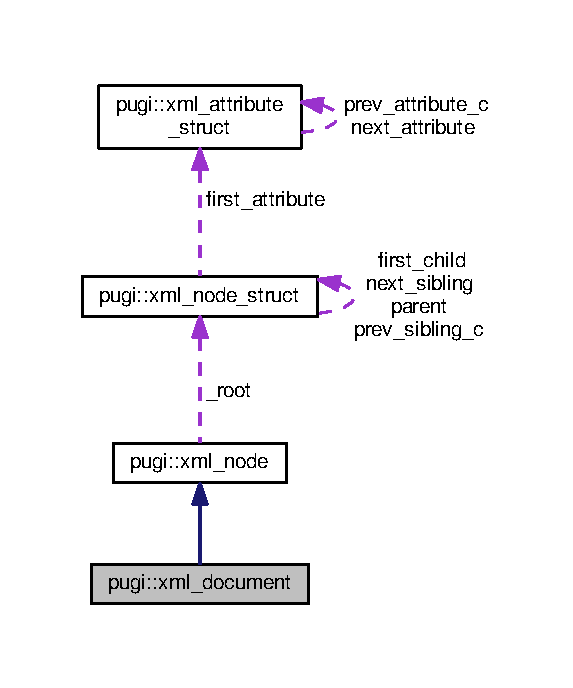
\includegraphics[width=275pt]{classpugi_1_1xml__document__coll__graph}
\end{center}
\end{figure}
\subsection*{Public Member Functions}
\begin{DoxyCompactItemize}
\item 
\hypertarget{classpugi_1_1xml__document_acf2b9daf1d12e12048796118b7a7685d}{void {\bfseries reset} ()}\label{classpugi_1_1xml__document_acf2b9daf1d12e12048796118b7a7685d}

\item 
\hypertarget{classpugi_1_1xml__document_a4230de3de88f4fe481c4c3d5312aa5cf}{void {\bfseries reset} (const \hyperlink{classpugi_1_1xml__document}{xml\+\_\+document} \&proto)}\label{classpugi_1_1xml__document_a4230de3de88f4fe481c4c3d5312aa5cf}

\item 
\hypertarget{classpugi_1_1xml__document_abb7db3882f94ac35b870510789a87778}{\hyperlink{structpugi_1_1xml__parse__result}{xml\+\_\+parse\+\_\+result} {\bfseries load} (std\+::basic\+\_\+istream$<$ char, std\+::char\+\_\+traits$<$ char $>$ $>$ \&stream, unsigned int options=parse\+\_\+default, xml\+\_\+encoding encoding=encoding\+\_\+auto)}\label{classpugi_1_1xml__document_abb7db3882f94ac35b870510789a87778}

\item 
\hypertarget{classpugi_1_1xml__document_a36131b6f1a80a1248666f4e7fe352685}{\hyperlink{structpugi_1_1xml__parse__result}{xml\+\_\+parse\+\_\+result} {\bfseries load} (std\+::basic\+\_\+istream$<$ wchar\+\_\+t, std\+::char\+\_\+traits$<$ wchar\+\_\+t $>$ $>$ \&stream, unsigned int options=parse\+\_\+default)}\label{classpugi_1_1xml__document_a36131b6f1a80a1248666f4e7fe352685}

\item 
\hypertarget{classpugi_1_1xml__document_ae17a77772fa21a40f3d91d9c79e60d0b}{\hyperlink{structpugi_1_1xml__parse__result}{xml\+\_\+parse\+\_\+result} {\bfseries load} (const char\+\_\+t $\ast$contents, unsigned int options=parse\+\_\+default)}\label{classpugi_1_1xml__document_ae17a77772fa21a40f3d91d9c79e60d0b}

\item 
\hypertarget{classpugi_1_1xml__document_a706a276ee3d5010f2bb8c7eacb75a891}{\hyperlink{structpugi_1_1xml__parse__result}{xml\+\_\+parse\+\_\+result} {\bfseries load\+\_\+string} (const char\+\_\+t $\ast$contents, unsigned int options=parse\+\_\+default)}\label{classpugi_1_1xml__document_a706a276ee3d5010f2bb8c7eacb75a891}

\item 
\hypertarget{classpugi_1_1xml__document_aad350209a4a91589fbd7e8cdaf79e010}{\hyperlink{structpugi_1_1xml__parse__result}{xml\+\_\+parse\+\_\+result} {\bfseries load\+\_\+file} (const char $\ast$path, unsigned int options=parse\+\_\+default, xml\+\_\+encoding encoding=encoding\+\_\+auto)}\label{classpugi_1_1xml__document_aad350209a4a91589fbd7e8cdaf79e010}

\item 
\hypertarget{classpugi_1_1xml__document_ac5a29d9c9e754120a5e0c072b332a25a}{\hyperlink{structpugi_1_1xml__parse__result}{xml\+\_\+parse\+\_\+result} {\bfseries load\+\_\+file} (const wchar\+\_\+t $\ast$path, unsigned int options=parse\+\_\+default, xml\+\_\+encoding encoding=encoding\+\_\+auto)}\label{classpugi_1_1xml__document_ac5a29d9c9e754120a5e0c072b332a25a}

\item 
\hypertarget{classpugi_1_1xml__document_ab29840790e26b2166a395c63a2b2d9bd}{\hyperlink{structpugi_1_1xml__parse__result}{xml\+\_\+parse\+\_\+result} {\bfseries load\+\_\+buffer} (const void $\ast$contents, size\+\_\+t size, unsigned int options=parse\+\_\+default, xml\+\_\+encoding encoding=encoding\+\_\+auto)}\label{classpugi_1_1xml__document_ab29840790e26b2166a395c63a2b2d9bd}

\item 
\hypertarget{classpugi_1_1xml__document_a3e20650182ccbdd175ca069dd5e08632}{\hyperlink{structpugi_1_1xml__parse__result}{xml\+\_\+parse\+\_\+result} {\bfseries load\+\_\+buffer\+\_\+inplace} (void $\ast$contents, size\+\_\+t size, unsigned int options=parse\+\_\+default, xml\+\_\+encoding encoding=encoding\+\_\+auto)}\label{classpugi_1_1xml__document_a3e20650182ccbdd175ca069dd5e08632}

\item 
\hypertarget{classpugi_1_1xml__document_a9da4bdcdc4ad914fb0f4680b02983502}{\hyperlink{structpugi_1_1xml__parse__result}{xml\+\_\+parse\+\_\+result} {\bfseries load\+\_\+buffer\+\_\+inplace\+\_\+own} (void $\ast$contents, size\+\_\+t size, unsigned int options=parse\+\_\+default, xml\+\_\+encoding encoding=encoding\+\_\+auto)}\label{classpugi_1_1xml__document_a9da4bdcdc4ad914fb0f4680b02983502}

\item 
\hypertarget{classpugi_1_1xml__document_ae69983f0991300cc9afc8891ff9ca4ac}{void {\bfseries save} (\hyperlink{classpugi_1_1xml__writer}{xml\+\_\+writer} \&writer, const char\+\_\+t $\ast$indent=P\+U\+G\+I\+X\+M\+L\+\_\+\+T\+E\+X\+T(\char`\"{}\textbackslash{}t\char`\"{}), unsigned int flags=format\+\_\+default, xml\+\_\+encoding encoding=encoding\+\_\+auto) const }\label{classpugi_1_1xml__document_ae69983f0991300cc9afc8891ff9ca4ac}

\item 
\hypertarget{classpugi_1_1xml__document_a471d7354af62da143f10943057c99ffa}{void {\bfseries save} (std\+::basic\+\_\+ostream$<$ char, std\+::char\+\_\+traits$<$ char $>$ $>$ \&stream, const char\+\_\+t $\ast$indent=P\+U\+G\+I\+X\+M\+L\+\_\+\+T\+E\+X\+T(\char`\"{}\textbackslash{}t\char`\"{}), unsigned int flags=format\+\_\+default, xml\+\_\+encoding encoding=encoding\+\_\+auto) const }\label{classpugi_1_1xml__document_a471d7354af62da143f10943057c99ffa}

\item 
\hypertarget{classpugi_1_1xml__document_ae0b377bda28c7fbac4ba50b4e3f9d211}{void {\bfseries save} (std\+::basic\+\_\+ostream$<$ wchar\+\_\+t, std\+::char\+\_\+traits$<$ wchar\+\_\+t $>$ $>$ \&stream, const char\+\_\+t $\ast$indent=P\+U\+G\+I\+X\+M\+L\+\_\+\+T\+E\+X\+T(\char`\"{}\textbackslash{}t\char`\"{}), unsigned int flags=format\+\_\+default) const }\label{classpugi_1_1xml__document_ae0b377bda28c7fbac4ba50b4e3f9d211}

\item 
\hypertarget{classpugi_1_1xml__document_ac67294573cbaa41d3e6210480a9f7f99}{bool {\bfseries save\+\_\+file} (const char $\ast$path, const char\+\_\+t $\ast$indent=P\+U\+G\+I\+X\+M\+L\+\_\+\+T\+E\+X\+T(\char`\"{}\textbackslash{}t\char`\"{}), unsigned int flags=format\+\_\+default, xml\+\_\+encoding encoding=encoding\+\_\+auto) const }\label{classpugi_1_1xml__document_ac67294573cbaa41d3e6210480a9f7f99}

\item 
\hypertarget{classpugi_1_1xml__document_a47e18cd3438eabd64fa2f82d56b08aef}{bool {\bfseries save\+\_\+file} (const wchar\+\_\+t $\ast$path, const char\+\_\+t $\ast$indent=P\+U\+G\+I\+X\+M\+L\+\_\+\+T\+E\+X\+T(\char`\"{}\textbackslash{}t\char`\"{}), unsigned int flags=format\+\_\+default, xml\+\_\+encoding encoding=encoding\+\_\+auto) const }\label{classpugi_1_1xml__document_a47e18cd3438eabd64fa2f82d56b08aef}

\item 
\hypertarget{classpugi_1_1xml__document_aa3b17a8891e2c89996ab4c7a2a6759ad}{\hyperlink{classpugi_1_1xml__node}{xml\+\_\+node} {\bfseries document\+\_\+element} () const }\label{classpugi_1_1xml__document_aa3b17a8891e2c89996ab4c7a2a6759ad}

\end{DoxyCompactItemize}
\subsection*{Additional Inherited Members}


The documentation for this class was generated from the following files\+:\begin{DoxyCompactItemize}
\item 
resources/pugixml-\/1.\+8/src/pugixml.\+hpp\item 
resources/pugixml-\/1.\+8/src/pugixml.\+cpp\end{DoxyCompactItemize}

\hypertarget{structxml__document__struct}{\section{xml\+\_\+document\+\_\+struct Struct Reference}
\label{structxml__document__struct}\index{xml\+\_\+document\+\_\+struct@{xml\+\_\+document\+\_\+struct}}
}


Inheritance diagram for xml\+\_\+document\+\_\+struct\+:
\nopagebreak
\begin{figure}[H]
\begin{center}
\leavevmode
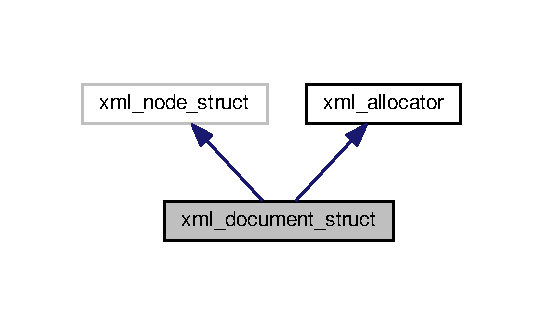
\includegraphics[width=261pt]{structxml__document__struct__inherit__graph}
\end{center}
\end{figure}


Collaboration diagram for xml\+\_\+document\+\_\+struct\+:
\nopagebreak
\begin{figure}[H]
\begin{center}
\leavevmode
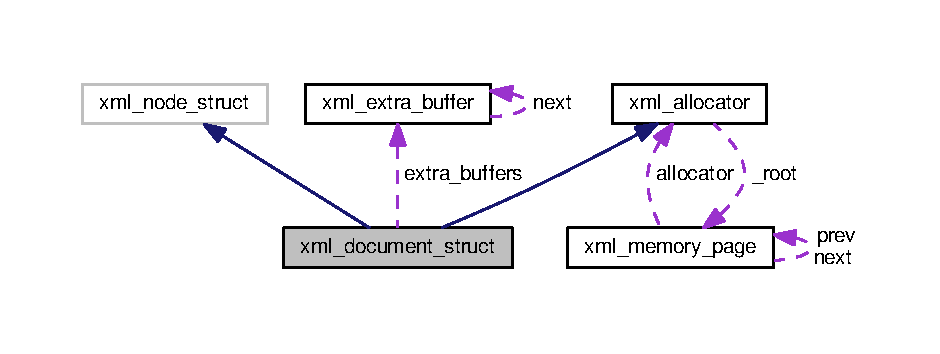
\includegraphics[width=350pt]{structxml__document__struct__coll__graph}
\end{center}
\end{figure}
\subsection*{Public Member Functions}
\begin{DoxyCompactItemize}
\item 
\hypertarget{structxml__document__struct_aea3482436c20abd98ca063c3bd5dcfba}{{\bfseries xml\+\_\+document\+\_\+struct} (\hyperlink{structxml__memory__page}{xml\+\_\+memory\+\_\+page} $\ast$page)}\label{structxml__document__struct_aea3482436c20abd98ca063c3bd5dcfba}

\end{DoxyCompactItemize}
\subsection*{Public Attributes}
\begin{DoxyCompactItemize}
\item 
\hypertarget{structxml__document__struct_a120451f29b8cc2a82a3ecc926449ea0e}{const char\+\_\+t $\ast$ {\bfseries buffer}}\label{structxml__document__struct_a120451f29b8cc2a82a3ecc926449ea0e}

\item 
\hypertarget{structxml__document__struct_afe3b1efd5b683c306157244496f55c4b}{\hyperlink{structxml__extra__buffer}{xml\+\_\+extra\+\_\+buffer} $\ast$ {\bfseries extra\+\_\+buffers}}\label{structxml__document__struct_afe3b1efd5b683c306157244496f55c4b}

\end{DoxyCompactItemize}
\subsection*{Additional Inherited Members}


The documentation for this struct was generated from the following file\+:\begin{DoxyCompactItemize}
\item 
resources/pugixml-\/1.\+8/src/pugixml.\+cpp\end{DoxyCompactItemize}

\hypertarget{structxml__extra__buffer}{\section{xml\+\_\+extra\+\_\+buffer Struct Reference}
\label{structxml__extra__buffer}\index{xml\+\_\+extra\+\_\+buffer@{xml\+\_\+extra\+\_\+buffer}}
}


Collaboration diagram for xml\+\_\+extra\+\_\+buffer\+:
\nopagebreak
\begin{figure}[H]
\begin{center}
\leavevmode
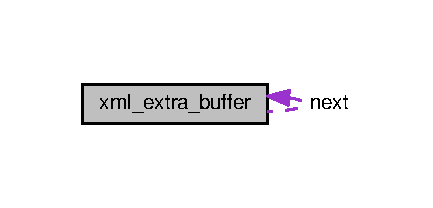
\includegraphics[width=208pt]{structxml__extra__buffer__coll__graph}
\end{center}
\end{figure}
\subsection*{Public Attributes}
\begin{DoxyCompactItemize}
\item 
\hypertarget{structxml__extra__buffer_ab24b191b25f92ad4d48009978ebee38c}{char\+\_\+t $\ast$ {\bfseries buffer}}\label{structxml__extra__buffer_ab24b191b25f92ad4d48009978ebee38c}

\item 
\hypertarget{structxml__extra__buffer_a8aaafa90868ca4d8e06b21eeabd96183}{\hyperlink{structxml__extra__buffer}{xml\+\_\+extra\+\_\+buffer} $\ast$ {\bfseries next}}\label{structxml__extra__buffer_a8aaafa90868ca4d8e06b21eeabd96183}

\end{DoxyCompactItemize}


The documentation for this struct was generated from the following file\+:\begin{DoxyCompactItemize}
\item 
resources/pugixml-\/1.\+8/src/pugixml.\+cpp\end{DoxyCompactItemize}

\hypertarget{structxml__memory__management__function__storage}{\section{xml\+\_\+memory\+\_\+management\+\_\+function\+\_\+storage$<$ T $>$ Struct Template Reference}
\label{structxml__memory__management__function__storage}\index{xml\+\_\+memory\+\_\+management\+\_\+function\+\_\+storage$<$ T $>$@{xml\+\_\+memory\+\_\+management\+\_\+function\+\_\+storage$<$ T $>$}}
}
\subsection*{Static Public Attributes}
\begin{DoxyCompactItemize}
\item 
\hypertarget{structxml__memory__management__function__storage_abb6865f8d07d27fd9273737c59f6e941}{static allocation\+\_\+function {\bfseries allocate} = default\+\_\+allocate}\label{structxml__memory__management__function__storage_abb6865f8d07d27fd9273737c59f6e941}

\item 
\hypertarget{structxml__memory__management__function__storage_a1c80a9a045ed6cfb90b17a178e4b3512}{static deallocation\+\_\+function {\bfseries deallocate} = default\+\_\+deallocate}\label{structxml__memory__management__function__storage_a1c80a9a045ed6cfb90b17a178e4b3512}

\end{DoxyCompactItemize}


The documentation for this struct was generated from the following file\+:\begin{DoxyCompactItemize}
\item 
resources/pugixml-\/1.\+8/src/pugixml.\+cpp\end{DoxyCompactItemize}

\hypertarget{structxml__memory__page}{\section{xml\+\_\+memory\+\_\+page Struct Reference}
\label{structxml__memory__page}\index{xml\+\_\+memory\+\_\+page@{xml\+\_\+memory\+\_\+page}}
}


Collaboration diagram for xml\+\_\+memory\+\_\+page\+:
\nopagebreak
\begin{figure}[H]
\begin{center}
\leavevmode
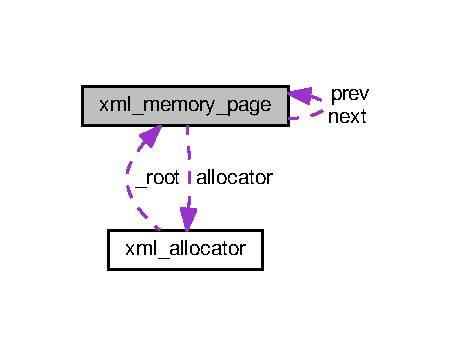
\includegraphics[width=218pt]{structxml__memory__page__coll__graph}
\end{center}
\end{figure}
\subsection*{Static Public Member Functions}
\begin{DoxyCompactItemize}
\item 
\hypertarget{structxml__memory__page_ab425973f2abb4fa98ff077d88c0df11c}{static \hyperlink{structxml__memory__page}{xml\+\_\+memory\+\_\+page} $\ast$ {\bfseries construct} (void $\ast$memory)}\label{structxml__memory__page_ab425973f2abb4fa98ff077d88c0df11c}

\end{DoxyCompactItemize}
\subsection*{Public Attributes}
\begin{DoxyCompactItemize}
\item 
\hypertarget{structxml__memory__page_adf8fa143123a842baa59b82fc3d83c3b}{\hyperlink{structxml__allocator}{xml\+\_\+allocator} $\ast$ {\bfseries allocator}}\label{structxml__memory__page_adf8fa143123a842baa59b82fc3d83c3b}

\item 
\hypertarget{structxml__memory__page_a014969b0e4a34a6cb24e9823791e60ab}{\hyperlink{structxml__memory__page}{xml\+\_\+memory\+\_\+page} $\ast$ {\bfseries prev}}\label{structxml__memory__page_a014969b0e4a34a6cb24e9823791e60ab}

\item 
\hypertarget{structxml__memory__page_a326a74e009af80219ea31bc65ed9e45e}{\hyperlink{structxml__memory__page}{xml\+\_\+memory\+\_\+page} $\ast$ {\bfseries next}}\label{structxml__memory__page_a326a74e009af80219ea31bc65ed9e45e}

\item 
\hypertarget{structxml__memory__page_a04780ddabc14b45baba3d1ded79d355a}{size\+\_\+t {\bfseries busy\+\_\+size}}\label{structxml__memory__page_a04780ddabc14b45baba3d1ded79d355a}

\item 
\hypertarget{structxml__memory__page_ab4c29645546530a0e1938b53979890a8}{size\+\_\+t {\bfseries freed\+\_\+size}}\label{structxml__memory__page_ab4c29645546530a0e1938b53979890a8}

\end{DoxyCompactItemize}


The documentation for this struct was generated from the following file\+:\begin{DoxyCompactItemize}
\item 
resources/pugixml-\/1.\+8/src/pugixml.\+cpp\end{DoxyCompactItemize}

\hypertarget{structxml__memory__string__header}{\section{xml\+\_\+memory\+\_\+string\+\_\+header Struct Reference}
\label{structxml__memory__string__header}\index{xml\+\_\+memory\+\_\+string\+\_\+header@{xml\+\_\+memory\+\_\+string\+\_\+header}}
}
\subsection*{Public Attributes}
\begin{DoxyCompactItemize}
\item 
\hypertarget{structxml__memory__string__header_a0cc274672f1263f73eeb6bf839bf96ee}{uint16\+\_\+t {\bfseries page\+\_\+offset}}\label{structxml__memory__string__header_a0cc274672f1263f73eeb6bf839bf96ee}

\item 
\hypertarget{structxml__memory__string__header_abbb48a709081e6610dffad322499e3f7}{uint16\+\_\+t {\bfseries full\+\_\+size}}\label{structxml__memory__string__header_abbb48a709081e6610dffad322499e3f7}

\end{DoxyCompactItemize}


The documentation for this struct was generated from the following file\+:\begin{DoxyCompactItemize}
\item 
resources/pugixml-\/1.\+8/src/pugixml.\+cpp\end{DoxyCompactItemize}

\hypertarget{structxml__memory__writer}{\section{xml\+\_\+memory\+\_\+writer Struct Reference}
\label{structxml__memory__writer}\index{xml\+\_\+memory\+\_\+writer@{xml\+\_\+memory\+\_\+writer}}
}


Inheritance diagram for xml\+\_\+memory\+\_\+writer\+:
\nopagebreak
\begin{figure}[H]
\begin{center}
\leavevmode
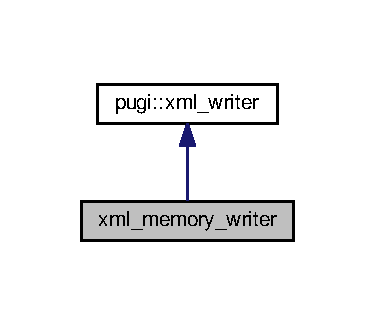
\includegraphics[width=180pt]{structxml__memory__writer__inherit__graph}
\end{center}
\end{figure}


Collaboration diagram for xml\+\_\+memory\+\_\+writer\+:
\nopagebreak
\begin{figure}[H]
\begin{center}
\leavevmode
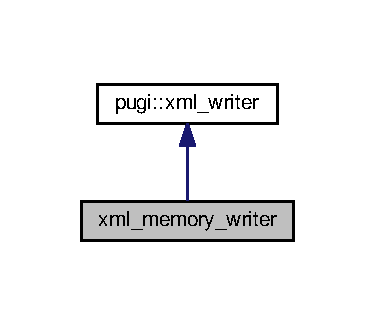
\includegraphics[width=180pt]{structxml__memory__writer__coll__graph}
\end{center}
\end{figure}
\subsection*{Public Member Functions}
\begin{DoxyCompactItemize}
\item 
\hypertarget{structxml__memory__writer_adbcc4bace05d4a174c24cb4731b32881}{{\bfseries xml\+\_\+memory\+\_\+writer} (char $\ast$buffer, size\+\_\+t capacity)}\label{structxml__memory__writer_adbcc4bace05d4a174c24cb4731b32881}

\item 
\hypertarget{structxml__memory__writer_a8f3b4725568f62ad17f7f138d9a76257}{size\+\_\+t {\bfseries written\+\_\+size} () const }\label{structxml__memory__writer_a8f3b4725568f62ad17f7f138d9a76257}

\item 
\hypertarget{structxml__memory__writer_a5b32fe490374a4539cd6b3d40a7876ef}{virtual void {\bfseries write} (const void $\ast$data, size\+\_\+t size)}\label{structxml__memory__writer_a5b32fe490374a4539cd6b3d40a7876ef}

\end{DoxyCompactItemize}
\subsection*{Public Attributes}
\begin{DoxyCompactItemize}
\item 
\hypertarget{structxml__memory__writer_a835b78d52bb768c3a67da998c2c17d72}{char $\ast$ {\bfseries buffer}}\label{structxml__memory__writer_a835b78d52bb768c3a67da998c2c17d72}

\item 
\hypertarget{structxml__memory__writer_aa389b21600101759566147b5ccb84d86}{size\+\_\+t {\bfseries capacity}}\label{structxml__memory__writer_aa389b21600101759566147b5ccb84d86}

\item 
\hypertarget{structxml__memory__writer_ad1ca31a422bbed9b1a0275f6a8647769}{size\+\_\+t {\bfseries result}}\label{structxml__memory__writer_ad1ca31a422bbed9b1a0275f6a8647769}

\end{DoxyCompactItemize}


The documentation for this struct was generated from the following file\+:\begin{DoxyCompactItemize}
\item 
resources/pugixml-\/1.\+8/docs/samples/save\+\_\+custom\+\_\+writer.\+cpp\end{DoxyCompactItemize}

\hypertarget{classpugi_1_1xml__named__node__iterator}{\section{pugi\+:\+:xml\+\_\+named\+\_\+node\+\_\+iterator Class Reference}
\label{classpugi_1_1xml__named__node__iterator}\index{pugi\+::xml\+\_\+named\+\_\+node\+\_\+iterator@{pugi\+::xml\+\_\+named\+\_\+node\+\_\+iterator}}
}
\subsection*{Public Types}
\begin{DoxyCompactItemize}
\item 
\hypertarget{classpugi_1_1xml__named__node__iterator_a18fa0d610fea4d64271729abc0e28849}{typedef ptrdiff\+\_\+t {\bfseries difference\+\_\+type}}\label{classpugi_1_1xml__named__node__iterator_a18fa0d610fea4d64271729abc0e28849}

\item 
\hypertarget{classpugi_1_1xml__named__node__iterator_a8d98d8218ea9740ceb990ef2c1a456e2}{typedef \hyperlink{classpugi_1_1xml__node}{xml\+\_\+node} {\bfseries value\+\_\+type}}\label{classpugi_1_1xml__named__node__iterator_a8d98d8218ea9740ceb990ef2c1a456e2}

\item 
\hypertarget{classpugi_1_1xml__named__node__iterator_aebf72c68ded20cf483a10c6b94aa3f57}{typedef \hyperlink{classpugi_1_1xml__node}{xml\+\_\+node} $\ast$ {\bfseries pointer}}\label{classpugi_1_1xml__named__node__iterator_aebf72c68ded20cf483a10c6b94aa3f57}

\item 
\hypertarget{classpugi_1_1xml__named__node__iterator_a1c338c7a2aefe04b83f746a963df808b}{typedef \hyperlink{classpugi_1_1xml__node}{xml\+\_\+node} \& {\bfseries reference}}\label{classpugi_1_1xml__named__node__iterator_a1c338c7a2aefe04b83f746a963df808b}

\item 
\hypertarget{classpugi_1_1xml__named__node__iterator_ab7dad0df34f043a9458b2a6b309a227f}{typedef \\*
std\+::bidirectional\+\_\+iterator\+\_\+tag {\bfseries iterator\+\_\+category}}\label{classpugi_1_1xml__named__node__iterator_ab7dad0df34f043a9458b2a6b309a227f}

\end{DoxyCompactItemize}
\subsection*{Public Member Functions}
\begin{DoxyCompactItemize}
\item 
\hypertarget{classpugi_1_1xml__named__node__iterator_a900cdc6c175bcb56b1c66c7c05d2202f}{{\bfseries xml\+\_\+named\+\_\+node\+\_\+iterator} (const \hyperlink{classpugi_1_1xml__node}{xml\+\_\+node} \&node, const char\+\_\+t $\ast$name)}\label{classpugi_1_1xml__named__node__iterator_a900cdc6c175bcb56b1c66c7c05d2202f}

\item 
\hypertarget{classpugi_1_1xml__named__node__iterator_a49533305b71d21a160dda111a2ed9956}{bool {\bfseries operator==} (const \hyperlink{classpugi_1_1xml__named__node__iterator}{xml\+\_\+named\+\_\+node\+\_\+iterator} \&rhs) const }\label{classpugi_1_1xml__named__node__iterator_a49533305b71d21a160dda111a2ed9956}

\item 
\hypertarget{classpugi_1_1xml__named__node__iterator_a3f625995e15f1b5debecdb9fb618c9d9}{bool {\bfseries operator!=} (const \hyperlink{classpugi_1_1xml__named__node__iterator}{xml\+\_\+named\+\_\+node\+\_\+iterator} \&rhs) const }\label{classpugi_1_1xml__named__node__iterator_a3f625995e15f1b5debecdb9fb618c9d9}

\item 
\hypertarget{classpugi_1_1xml__named__node__iterator_a382a1fe2474c25b47d96dd901e3add8a}{\hyperlink{classpugi_1_1xml__node}{xml\+\_\+node} \& {\bfseries operator$\ast$} () const }\label{classpugi_1_1xml__named__node__iterator_a382a1fe2474c25b47d96dd901e3add8a}

\item 
\hypertarget{classpugi_1_1xml__named__node__iterator_a9fa4ca35803bfd50c61d369241a3da4a}{\hyperlink{classpugi_1_1xml__node}{xml\+\_\+node} $\ast$ {\bfseries operator-\/$>$} () const }\label{classpugi_1_1xml__named__node__iterator_a9fa4ca35803bfd50c61d369241a3da4a}

\item 
\hypertarget{classpugi_1_1xml__named__node__iterator_ae076ec9c8414c5444ce6e4db5052ccef}{const \hyperlink{classpugi_1_1xml__named__node__iterator}{xml\+\_\+named\+\_\+node\+\_\+iterator} \& {\bfseries operator++} ()}\label{classpugi_1_1xml__named__node__iterator_ae076ec9c8414c5444ce6e4db5052ccef}

\item 
\hypertarget{classpugi_1_1xml__named__node__iterator_a41e2afe0ee62a2d06d0694052277e1f9}{\hyperlink{classpugi_1_1xml__named__node__iterator}{xml\+\_\+named\+\_\+node\+\_\+iterator} {\bfseries operator++} (int)}\label{classpugi_1_1xml__named__node__iterator_a41e2afe0ee62a2d06d0694052277e1f9}

\item 
\hypertarget{classpugi_1_1xml__named__node__iterator_aaee9df71be9b3a08f871cbf420d8384d}{const \hyperlink{classpugi_1_1xml__named__node__iterator}{xml\+\_\+named\+\_\+node\+\_\+iterator} \& {\bfseries operator-\/-\/} ()}\label{classpugi_1_1xml__named__node__iterator_aaee9df71be9b3a08f871cbf420d8384d}

\item 
\hypertarget{classpugi_1_1xml__named__node__iterator_af5b1c61a813276537774d60e32c6408c}{\hyperlink{classpugi_1_1xml__named__node__iterator}{xml\+\_\+named\+\_\+node\+\_\+iterator} {\bfseries operator-\/-\/} (int)}\label{classpugi_1_1xml__named__node__iterator_af5b1c61a813276537774d60e32c6408c}

\end{DoxyCompactItemize}
\subsection*{Friends}
\begin{DoxyCompactItemize}
\item 
\hypertarget{classpugi_1_1xml__named__node__iterator_a156d917a92815c7b593bd5ef19f6d5fb}{class {\bfseries xml\+\_\+node}}\label{classpugi_1_1xml__named__node__iterator_a156d917a92815c7b593bd5ef19f6d5fb}

\end{DoxyCompactItemize}


The documentation for this class was generated from the following files\+:\begin{DoxyCompactItemize}
\item 
resources/pugixml-\/1.\+8/src/pugixml.\+hpp\item 
resources/pugixml-\/1.\+8/src/pugixml.\+cpp\end{DoxyCompactItemize}

\hypertarget{classpugi_1_1xml__node}{\section{pugi\+:\+:xml\+\_\+node Class Reference}
\label{classpugi_1_1xml__node}\index{pugi\+::xml\+\_\+node@{pugi\+::xml\+\_\+node}}
}


Inheritance diagram for pugi\+:\+:xml\+\_\+node\+:
\nopagebreak
\begin{figure}[H]
\begin{center}
\leavevmode
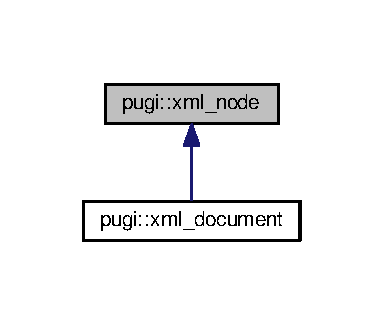
\includegraphics[width=184pt]{classpugi_1_1xml__node__inherit__graph}
\end{center}
\end{figure}


Collaboration diagram for pugi\+:\+:xml\+\_\+node\+:
\nopagebreak
\begin{figure}[H]
\begin{center}
\leavevmode
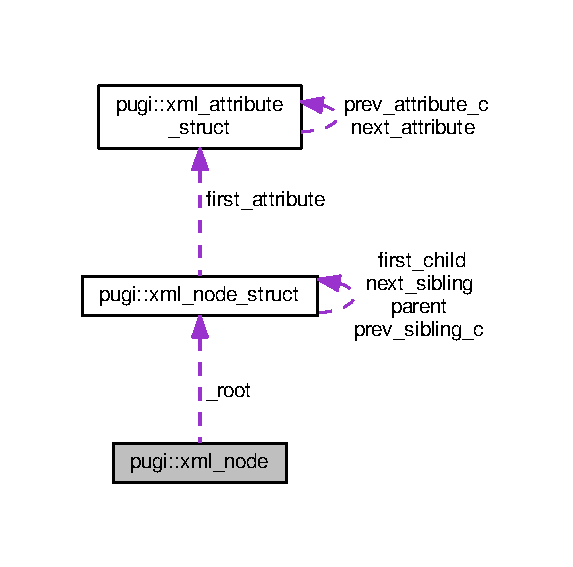
\includegraphics[width=275pt]{classpugi_1_1xml__node__coll__graph}
\end{center}
\end{figure}
\subsection*{Public Types}
\begin{DoxyCompactItemize}
\item 
\hypertarget{classpugi_1_1xml__node_ae053ea39add5a64de584f7a81212e388}{typedef \hyperlink{classpugi_1_1xml__node__iterator}{xml\+\_\+node\+\_\+iterator} {\bfseries iterator}}\label{classpugi_1_1xml__node_ae053ea39add5a64de584f7a81212e388}

\item 
\hypertarget{classpugi_1_1xml__node_a9084f97350ffc64af1eaf7c17c57f4ba}{typedef \hyperlink{classpugi_1_1xml__attribute__iterator}{xml\+\_\+attribute\+\_\+iterator} {\bfseries attribute\+\_\+iterator}}\label{classpugi_1_1xml__node_a9084f97350ffc64af1eaf7c17c57f4ba}

\end{DoxyCompactItemize}
\subsection*{Public Member Functions}
\begin{DoxyCompactItemize}
\item 
\hypertarget{classpugi_1_1xml__node_afc9b1ed8891dfed9ce5ab5288a9ad4a1}{{\bfseries xml\+\_\+node} (\hyperlink{structpugi_1_1xml__node__struct}{xml\+\_\+node\+\_\+struct} $\ast$p)}\label{classpugi_1_1xml__node_afc9b1ed8891dfed9ce5ab5288a9ad4a1}

\item 
\hypertarget{classpugi_1_1xml__node_af30001c73a3454a1e3794a850d3963c0}{{\bfseries operator unspecified\+\_\+bool\+\_\+type} () const }\label{classpugi_1_1xml__node_af30001c73a3454a1e3794a850d3963c0}

\item 
\hypertarget{classpugi_1_1xml__node_a03c028fd83e07cda3f433f9eea3466ff}{bool {\bfseries operator!} () const }\label{classpugi_1_1xml__node_a03c028fd83e07cda3f433f9eea3466ff}

\item 
\hypertarget{classpugi_1_1xml__node_aaf46fa45a1a117ca95867f37ade363c2}{bool {\bfseries operator==} (const \hyperlink{classpugi_1_1xml__node}{xml\+\_\+node} \&r) const }\label{classpugi_1_1xml__node_aaf46fa45a1a117ca95867f37ade363c2}

\item 
\hypertarget{classpugi_1_1xml__node_aa31095e51422a8a11b8d4832e0db71ed}{bool {\bfseries operator!=} (const \hyperlink{classpugi_1_1xml__node}{xml\+\_\+node} \&r) const }\label{classpugi_1_1xml__node_aa31095e51422a8a11b8d4832e0db71ed}

\item 
\hypertarget{classpugi_1_1xml__node_a2a57731a8d90392f88febf551bd5a924}{bool {\bfseries operator$<$} (const \hyperlink{classpugi_1_1xml__node}{xml\+\_\+node} \&r) const }\label{classpugi_1_1xml__node_a2a57731a8d90392f88febf551bd5a924}

\item 
\hypertarget{classpugi_1_1xml__node_a983e49938a893181fd8cc905c4c67f64}{bool {\bfseries operator$>$} (const \hyperlink{classpugi_1_1xml__node}{xml\+\_\+node} \&r) const }\label{classpugi_1_1xml__node_a983e49938a893181fd8cc905c4c67f64}

\item 
\hypertarget{classpugi_1_1xml__node_a09568e579d8c1b6bff12594bfb4246b6}{bool {\bfseries operator$<$=} (const \hyperlink{classpugi_1_1xml__node}{xml\+\_\+node} \&r) const }\label{classpugi_1_1xml__node_a09568e579d8c1b6bff12594bfb4246b6}

\item 
\hypertarget{classpugi_1_1xml__node_a8c89c4333fdd22f19714a945895d2e39}{bool {\bfseries operator$>$=} (const \hyperlink{classpugi_1_1xml__node}{xml\+\_\+node} \&r) const }\label{classpugi_1_1xml__node_a8c89c4333fdd22f19714a945895d2e39}

\item 
\hypertarget{classpugi_1_1xml__node_a2c416c45fcd27a9cf4e7914d560a0cc4}{bool {\bfseries empty} () const }\label{classpugi_1_1xml__node_a2c416c45fcd27a9cf4e7914d560a0cc4}

\item 
\hypertarget{classpugi_1_1xml__node_ab881e8c41edc84bf7507591d1ad8ead4}{xml\+\_\+node\+\_\+type {\bfseries type} () const }\label{classpugi_1_1xml__node_ab881e8c41edc84bf7507591d1ad8ead4}

\item 
\hypertarget{classpugi_1_1xml__node_ac765caace42ecf252d90aea81e09df57}{const char\+\_\+t $\ast$ {\bfseries name} () const }\label{classpugi_1_1xml__node_ac765caace42ecf252d90aea81e09df57}

\item 
\hypertarget{classpugi_1_1xml__node_a3e7e935a101432fd4f6dcaf6bfb495d4}{const char\+\_\+t $\ast$ {\bfseries value} () const }\label{classpugi_1_1xml__node_a3e7e935a101432fd4f6dcaf6bfb495d4}

\item 
\hypertarget{classpugi_1_1xml__node_ac53e177390f1f73e6cef4f5be3ecaa9d}{\hyperlink{classpugi_1_1xml__attribute}{xml\+\_\+attribute} {\bfseries first\+\_\+attribute} () const }\label{classpugi_1_1xml__node_ac53e177390f1f73e6cef4f5be3ecaa9d}

\item 
\hypertarget{classpugi_1_1xml__node_a10695e006b24e726ba313d5554086802}{\hyperlink{classpugi_1_1xml__attribute}{xml\+\_\+attribute} {\bfseries last\+\_\+attribute} () const }\label{classpugi_1_1xml__node_a10695e006b24e726ba313d5554086802}

\item 
\hypertarget{classpugi_1_1xml__node_a71641cb34be57df1b25e2df7eac31f00}{\hyperlink{classpugi_1_1xml__node}{xml\+\_\+node} {\bfseries first\+\_\+child} () const }\label{classpugi_1_1xml__node_a71641cb34be57df1b25e2df7eac31f00}

\item 
\hypertarget{classpugi_1_1xml__node_a076b2868a97458d5abeeec9e6c433244}{\hyperlink{classpugi_1_1xml__node}{xml\+\_\+node} {\bfseries last\+\_\+child} () const }\label{classpugi_1_1xml__node_a076b2868a97458d5abeeec9e6c433244}

\item 
\hypertarget{classpugi_1_1xml__node_a713159ab981fb3f0a325434106dc94f5}{\hyperlink{classpugi_1_1xml__node}{xml\+\_\+node} {\bfseries next\+\_\+sibling} () const }\label{classpugi_1_1xml__node_a713159ab981fb3f0a325434106dc94f5}

\item 
\hypertarget{classpugi_1_1xml__node_a367e7e2c78a3870aad7ad3831da7c0fa}{\hyperlink{classpugi_1_1xml__node}{xml\+\_\+node} {\bfseries previous\+\_\+sibling} () const }\label{classpugi_1_1xml__node_a367e7e2c78a3870aad7ad3831da7c0fa}

\item 
\hypertarget{classpugi_1_1xml__node_a5c7a1b2ec89d59afa1028e9c5fc25640}{\hyperlink{classpugi_1_1xml__node}{xml\+\_\+node} {\bfseries parent} () const }\label{classpugi_1_1xml__node_a5c7a1b2ec89d59afa1028e9c5fc25640}

\item 
\hypertarget{classpugi_1_1xml__node_a713b60fd5cddd5d8671dd76b1457e6eb}{\hyperlink{classpugi_1_1xml__node}{xml\+\_\+node} {\bfseries root} () const }\label{classpugi_1_1xml__node_a713b60fd5cddd5d8671dd76b1457e6eb}

\item 
\hypertarget{classpugi_1_1xml__node_aafe1c1c7cd27f3c9c758b517abc7886a}{\hyperlink{classpugi_1_1xml__text}{xml\+\_\+text} {\bfseries text} () const }\label{classpugi_1_1xml__node_aafe1c1c7cd27f3c9c758b517abc7886a}

\item 
\hypertarget{classpugi_1_1xml__node_af3aa192b114a289640110c9e4da020ca}{\hyperlink{classpugi_1_1xml__node}{xml\+\_\+node} {\bfseries child} (const char\+\_\+t $\ast$name) const }\label{classpugi_1_1xml__node_af3aa192b114a289640110c9e4da020ca}

\item 
\hypertarget{classpugi_1_1xml__node_a19fc1a285c0f751f52c0e151a727de97}{\hyperlink{classpugi_1_1xml__attribute}{xml\+\_\+attribute} {\bfseries attribute} (const char\+\_\+t $\ast$name) const }\label{classpugi_1_1xml__node_a19fc1a285c0f751f52c0e151a727de97}

\item 
\hypertarget{classpugi_1_1xml__node_a51a25d1e6f2315b65a1f969126cbc612}{\hyperlink{classpugi_1_1xml__node}{xml\+\_\+node} {\bfseries next\+\_\+sibling} (const char\+\_\+t $\ast$name) const }\label{classpugi_1_1xml__node_a51a25d1e6f2315b65a1f969126cbc612}

\item 
\hypertarget{classpugi_1_1xml__node_a311405d1ee4a564071a5f44b476b05f7}{\hyperlink{classpugi_1_1xml__node}{xml\+\_\+node} {\bfseries previous\+\_\+sibling} (const char\+\_\+t $\ast$name) const }\label{classpugi_1_1xml__node_a311405d1ee4a564071a5f44b476b05f7}

\item 
\hypertarget{classpugi_1_1xml__node_adba5080f639116c53b5555c3582acfaf}{\hyperlink{classpugi_1_1xml__attribute}{xml\+\_\+attribute} {\bfseries attribute} (const char\+\_\+t $\ast$name, \hyperlink{classpugi_1_1xml__attribute}{xml\+\_\+attribute} \&hint) const }\label{classpugi_1_1xml__node_adba5080f639116c53b5555c3582acfaf}

\item 
\hypertarget{classpugi_1_1xml__node_a1c824a58d4c591c0da8f5dc39938456f}{const char\+\_\+t $\ast$ {\bfseries child\+\_\+value} () const }\label{classpugi_1_1xml__node_a1c824a58d4c591c0da8f5dc39938456f}

\item 
\hypertarget{classpugi_1_1xml__node_ad091dcc0ff970fb2920b8b2942154c94}{const char\+\_\+t $\ast$ {\bfseries child\+\_\+value} (const char\+\_\+t $\ast$name) const }\label{classpugi_1_1xml__node_ad091dcc0ff970fb2920b8b2942154c94}

\item 
\hypertarget{classpugi_1_1xml__node_a9d688489fcf0960e945a12480419e434}{bool {\bfseries set\+\_\+name} (const char\+\_\+t $\ast$rhs)}\label{classpugi_1_1xml__node_a9d688489fcf0960e945a12480419e434}

\item 
\hypertarget{classpugi_1_1xml__node_a160f1fa7a0eda1e5ad9d19d45f6b0e4e}{bool {\bfseries set\+\_\+value} (const char\+\_\+t $\ast$rhs)}\label{classpugi_1_1xml__node_a160f1fa7a0eda1e5ad9d19d45f6b0e4e}

\item 
\hypertarget{classpugi_1_1xml__node_a417eb03f034b432bb2800e54e38022aa}{\hyperlink{classpugi_1_1xml__attribute}{xml\+\_\+attribute} {\bfseries append\+\_\+attribute} (const char\+\_\+t $\ast$name)}\label{classpugi_1_1xml__node_a417eb03f034b432bb2800e54e38022aa}

\item 
\hypertarget{classpugi_1_1xml__node_a7d70631d6cb3624cdfc4cf9ef4abad06}{\hyperlink{classpugi_1_1xml__attribute}{xml\+\_\+attribute} {\bfseries prepend\+\_\+attribute} (const char\+\_\+t $\ast$name)}\label{classpugi_1_1xml__node_a7d70631d6cb3624cdfc4cf9ef4abad06}

\item 
\hypertarget{classpugi_1_1xml__node_a74ab20fa84dffde317f8899af628f041}{\hyperlink{classpugi_1_1xml__attribute}{xml\+\_\+attribute} {\bfseries insert\+\_\+attribute\+\_\+after} (const char\+\_\+t $\ast$name, const \hyperlink{classpugi_1_1xml__attribute}{xml\+\_\+attribute} \&attr)}\label{classpugi_1_1xml__node_a74ab20fa84dffde317f8899af628f041}

\item 
\hypertarget{classpugi_1_1xml__node_a742898bc2342d943a4c49916ac3a64b8}{\hyperlink{classpugi_1_1xml__attribute}{xml\+\_\+attribute} {\bfseries insert\+\_\+attribute\+\_\+before} (const char\+\_\+t $\ast$name, const \hyperlink{classpugi_1_1xml__attribute}{xml\+\_\+attribute} \&attr)}\label{classpugi_1_1xml__node_a742898bc2342d943a4c49916ac3a64b8}

\item 
\hypertarget{classpugi_1_1xml__node_a4c151e6665c6bfa614fe80d177fd5396}{\hyperlink{classpugi_1_1xml__attribute}{xml\+\_\+attribute} {\bfseries append\+\_\+copy} (const \hyperlink{classpugi_1_1xml__attribute}{xml\+\_\+attribute} \&proto)}\label{classpugi_1_1xml__node_a4c151e6665c6bfa614fe80d177fd5396}

\item 
\hypertarget{classpugi_1_1xml__node_abd0f80e4d5bc938a27b50d37a0c7865b}{\hyperlink{classpugi_1_1xml__attribute}{xml\+\_\+attribute} {\bfseries prepend\+\_\+copy} (const \hyperlink{classpugi_1_1xml__attribute}{xml\+\_\+attribute} \&proto)}\label{classpugi_1_1xml__node_abd0f80e4d5bc938a27b50d37a0c7865b}

\item 
\hypertarget{classpugi_1_1xml__node_ab5fd2ccada30141544b12c6ef554d8f4}{\hyperlink{classpugi_1_1xml__attribute}{xml\+\_\+attribute} {\bfseries insert\+\_\+copy\+\_\+after} (const \hyperlink{classpugi_1_1xml__attribute}{xml\+\_\+attribute} \&proto, const \hyperlink{classpugi_1_1xml__attribute}{xml\+\_\+attribute} \&attr)}\label{classpugi_1_1xml__node_ab5fd2ccada30141544b12c6ef554d8f4}

\item 
\hypertarget{classpugi_1_1xml__node_ac81f8aded4b53a9b8c98d131986cb535}{\hyperlink{classpugi_1_1xml__attribute}{xml\+\_\+attribute} {\bfseries insert\+\_\+copy\+\_\+before} (const \hyperlink{classpugi_1_1xml__attribute}{xml\+\_\+attribute} \&proto, const \hyperlink{classpugi_1_1xml__attribute}{xml\+\_\+attribute} \&attr)}\label{classpugi_1_1xml__node_ac81f8aded4b53a9b8c98d131986cb535}

\item 
\hypertarget{classpugi_1_1xml__node_a190f4851bb4bc4bb61c89fffb663a9af}{\hyperlink{classpugi_1_1xml__node}{xml\+\_\+node} {\bfseries append\+\_\+child} (xml\+\_\+node\+\_\+type type=node\+\_\+element)}\label{classpugi_1_1xml__node_a190f4851bb4bc4bb61c89fffb663a9af}

\item 
\hypertarget{classpugi_1_1xml__node_a9e0a6dddfe1fefc74bb2b7689376989c}{\hyperlink{classpugi_1_1xml__node}{xml\+\_\+node} {\bfseries prepend\+\_\+child} (xml\+\_\+node\+\_\+type type=node\+\_\+element)}\label{classpugi_1_1xml__node_a9e0a6dddfe1fefc74bb2b7689376989c}

\item 
\hypertarget{classpugi_1_1xml__node_a4dd8d25c02560a2692c43cc4779fb7e3}{\hyperlink{classpugi_1_1xml__node}{xml\+\_\+node} {\bfseries insert\+\_\+child\+\_\+after} (xml\+\_\+node\+\_\+type type, const \hyperlink{classpugi_1_1xml__node}{xml\+\_\+node} \&node)}\label{classpugi_1_1xml__node_a4dd8d25c02560a2692c43cc4779fb7e3}

\item 
\hypertarget{classpugi_1_1xml__node_afe89f53c01eac8209b06f9fe7f84e7c1}{\hyperlink{classpugi_1_1xml__node}{xml\+\_\+node} {\bfseries insert\+\_\+child\+\_\+before} (xml\+\_\+node\+\_\+type type, const \hyperlink{classpugi_1_1xml__node}{xml\+\_\+node} \&node)}\label{classpugi_1_1xml__node_afe89f53c01eac8209b06f9fe7f84e7c1}

\item 
\hypertarget{classpugi_1_1xml__node_a448342425806a4ad8068bf98fd4ff462}{\hyperlink{classpugi_1_1xml__node}{xml\+\_\+node} {\bfseries append\+\_\+child} (const char\+\_\+t $\ast$name)}\label{classpugi_1_1xml__node_a448342425806a4ad8068bf98fd4ff462}

\item 
\hypertarget{classpugi_1_1xml__node_afa78286431f99a0f35b18185e11e28e8}{\hyperlink{classpugi_1_1xml__node}{xml\+\_\+node} {\bfseries prepend\+\_\+child} (const char\+\_\+t $\ast$name)}\label{classpugi_1_1xml__node_afa78286431f99a0f35b18185e11e28e8}

\item 
\hypertarget{classpugi_1_1xml__node_a778c2246fef9964b2d947253a86f2982}{\hyperlink{classpugi_1_1xml__node}{xml\+\_\+node} {\bfseries insert\+\_\+child\+\_\+after} (const char\+\_\+t $\ast$name, const \hyperlink{classpugi_1_1xml__node}{xml\+\_\+node} \&node)}\label{classpugi_1_1xml__node_a778c2246fef9964b2d947253a86f2982}

\item 
\hypertarget{classpugi_1_1xml__node_a70fa68762aed11c82a1b913571df4394}{\hyperlink{classpugi_1_1xml__node}{xml\+\_\+node} {\bfseries insert\+\_\+child\+\_\+before} (const char\+\_\+t $\ast$name, const \hyperlink{classpugi_1_1xml__node}{xml\+\_\+node} \&node)}\label{classpugi_1_1xml__node_a70fa68762aed11c82a1b913571df4394}

\item 
\hypertarget{classpugi_1_1xml__node_a17971e2b69c4dd4f45c461ebffe96732}{\hyperlink{classpugi_1_1xml__node}{xml\+\_\+node} {\bfseries append\+\_\+copy} (const \hyperlink{classpugi_1_1xml__node}{xml\+\_\+node} \&proto)}\label{classpugi_1_1xml__node_a17971e2b69c4dd4f45c461ebffe96732}

\item 
\hypertarget{classpugi_1_1xml__node_a29cc787ee2270e3a71e1d511164621e6}{\hyperlink{classpugi_1_1xml__node}{xml\+\_\+node} {\bfseries prepend\+\_\+copy} (const \hyperlink{classpugi_1_1xml__node}{xml\+\_\+node} \&proto)}\label{classpugi_1_1xml__node_a29cc787ee2270e3a71e1d511164621e6}

\item 
\hypertarget{classpugi_1_1xml__node_a106a600eac7d08608f797d034b331fa8}{\hyperlink{classpugi_1_1xml__node}{xml\+\_\+node} {\bfseries insert\+\_\+copy\+\_\+after} (const \hyperlink{classpugi_1_1xml__node}{xml\+\_\+node} \&proto, const \hyperlink{classpugi_1_1xml__node}{xml\+\_\+node} \&node)}\label{classpugi_1_1xml__node_a106a600eac7d08608f797d034b331fa8}

\item 
\hypertarget{classpugi_1_1xml__node_a21134448747e00888df7ecfb174032d3}{\hyperlink{classpugi_1_1xml__node}{xml\+\_\+node} {\bfseries insert\+\_\+copy\+\_\+before} (const \hyperlink{classpugi_1_1xml__node}{xml\+\_\+node} \&proto, const \hyperlink{classpugi_1_1xml__node}{xml\+\_\+node} \&node)}\label{classpugi_1_1xml__node_a21134448747e00888df7ecfb174032d3}

\item 
\hypertarget{classpugi_1_1xml__node_a25af08bf4e45d2b0380328a0d9d08960}{\hyperlink{classpugi_1_1xml__node}{xml\+\_\+node} {\bfseries append\+\_\+move} (const \hyperlink{classpugi_1_1xml__node}{xml\+\_\+node} \&moved)}\label{classpugi_1_1xml__node_a25af08bf4e45d2b0380328a0d9d08960}

\item 
\hypertarget{classpugi_1_1xml__node_a400191f234f22efd0379e68700bf9650}{\hyperlink{classpugi_1_1xml__node}{xml\+\_\+node} {\bfseries prepend\+\_\+move} (const \hyperlink{classpugi_1_1xml__node}{xml\+\_\+node} \&moved)}\label{classpugi_1_1xml__node_a400191f234f22efd0379e68700bf9650}

\item 
\hypertarget{classpugi_1_1xml__node_a23ad17b7d7539169537d95f1fd1ec9b1}{\hyperlink{classpugi_1_1xml__node}{xml\+\_\+node} {\bfseries insert\+\_\+move\+\_\+after} (const \hyperlink{classpugi_1_1xml__node}{xml\+\_\+node} \&moved, const \hyperlink{classpugi_1_1xml__node}{xml\+\_\+node} \&node)}\label{classpugi_1_1xml__node_a23ad17b7d7539169537d95f1fd1ec9b1}

\item 
\hypertarget{classpugi_1_1xml__node_abf67ad284bfbdf8bc401e24b086cf45e}{\hyperlink{classpugi_1_1xml__node}{xml\+\_\+node} {\bfseries insert\+\_\+move\+\_\+before} (const \hyperlink{classpugi_1_1xml__node}{xml\+\_\+node} \&moved, const \hyperlink{classpugi_1_1xml__node}{xml\+\_\+node} \&node)}\label{classpugi_1_1xml__node_abf67ad284bfbdf8bc401e24b086cf45e}

\item 
\hypertarget{classpugi_1_1xml__node_aee02f0e2dab4aaeb6196f26b3bcf258c}{bool {\bfseries remove\+\_\+attribute} (const \hyperlink{classpugi_1_1xml__attribute}{xml\+\_\+attribute} \&a)}\label{classpugi_1_1xml__node_aee02f0e2dab4aaeb6196f26b3bcf258c}

\item 
\hypertarget{classpugi_1_1xml__node_a2625858b335a1289d72d19b57acc639c}{bool {\bfseries remove\+\_\+attribute} (const char\+\_\+t $\ast$name)}\label{classpugi_1_1xml__node_a2625858b335a1289d72d19b57acc639c}

\item 
\hypertarget{classpugi_1_1xml__node_a4b562d01edab7dad880e9e297203843d}{bool {\bfseries remove\+\_\+child} (const \hyperlink{classpugi_1_1xml__node}{xml\+\_\+node} \&n)}\label{classpugi_1_1xml__node_a4b562d01edab7dad880e9e297203843d}

\item 
\hypertarget{classpugi_1_1xml__node_a1930157197e41cc15eea1fc00eecf1dd}{bool {\bfseries remove\+\_\+child} (const char\+\_\+t $\ast$name)}\label{classpugi_1_1xml__node_a1930157197e41cc15eea1fc00eecf1dd}

\item 
\hypertarget{classpugi_1_1xml__node_a7e0126c503dcfba5111121ec4a94c11e}{\hyperlink{structpugi_1_1xml__parse__result}{xml\+\_\+parse\+\_\+result} {\bfseries append\+\_\+buffer} (const void $\ast$contents, size\+\_\+t size, unsigned int options=parse\+\_\+default, xml\+\_\+encoding encoding=encoding\+\_\+auto)}\label{classpugi_1_1xml__node_a7e0126c503dcfba5111121ec4a94c11e}

\item 
\hypertarget{classpugi_1_1xml__node_a4e0125eb6c0857df370119df923096ea}{{\footnotesize template$<$typename Predicate $>$ }\\\hyperlink{classpugi_1_1xml__attribute}{xml\+\_\+attribute} {\bfseries find\+\_\+attribute} (Predicate pred) const }\label{classpugi_1_1xml__node_a4e0125eb6c0857df370119df923096ea}

\item 
\hypertarget{classpugi_1_1xml__node_a25b60f2847c1937f0d4dbd4828bdcd7d}{{\footnotesize template$<$typename Predicate $>$ }\\\hyperlink{classpugi_1_1xml__node}{xml\+\_\+node} {\bfseries find\+\_\+child} (Predicate pred) const }\label{classpugi_1_1xml__node_a25b60f2847c1937f0d4dbd4828bdcd7d}

\item 
\hypertarget{classpugi_1_1xml__node_a28ccb61937080e9cefe991a0c6837be6}{{\footnotesize template$<$typename Predicate $>$ }\\\hyperlink{classpugi_1_1xml__node}{xml\+\_\+node} {\bfseries find\+\_\+node} (Predicate pred) const }\label{classpugi_1_1xml__node_a28ccb61937080e9cefe991a0c6837be6}

\item 
\hypertarget{classpugi_1_1xml__node_adcbe6392a84e4d156cca69c8ec3224da}{\hyperlink{classpugi_1_1xml__node}{xml\+\_\+node} {\bfseries find\+\_\+child\+\_\+by\+\_\+attribute} (const char\+\_\+t $\ast$name, const char\+\_\+t $\ast$attr\+\_\+name, const char\+\_\+t $\ast$attr\+\_\+value) const }\label{classpugi_1_1xml__node_adcbe6392a84e4d156cca69c8ec3224da}

\item 
\hypertarget{classpugi_1_1xml__node_a96377b213e80a99cc21db911610b88e0}{\hyperlink{classpugi_1_1xml__node}{xml\+\_\+node} {\bfseries find\+\_\+child\+\_\+by\+\_\+attribute} (const char\+\_\+t $\ast$attr\+\_\+name, const char\+\_\+t $\ast$attr\+\_\+value) const }\label{classpugi_1_1xml__node_a96377b213e80a99cc21db911610b88e0}

\item 
\hypertarget{classpugi_1_1xml__node_ae5694be88058346ad8e6e418410d4979}{string\+\_\+t {\bfseries path} (char\+\_\+t delimiter= '/') const }\label{classpugi_1_1xml__node_ae5694be88058346ad8e6e418410d4979}

\item 
\hypertarget{classpugi_1_1xml__node_ae701cc3920f4a779610f94219bb41fe1}{\hyperlink{classpugi_1_1xml__node}{xml\+\_\+node} {\bfseries first\+\_\+element\+\_\+by\+\_\+path} (const char\+\_\+t $\ast$path, char\+\_\+t delimiter= '/') const }\label{classpugi_1_1xml__node_ae701cc3920f4a779610f94219bb41fe1}

\item 
\hypertarget{classpugi_1_1xml__node_a951d5d02987f75fabc4d575cfdeec8b4}{bool {\bfseries traverse} (\hyperlink{classpugi_1_1xml__tree__walker}{xml\+\_\+tree\+\_\+walker} \&walker)}\label{classpugi_1_1xml__node_a951d5d02987f75fabc4d575cfdeec8b4}

\item 
\hypertarget{classpugi_1_1xml__node_a87dc7d267f7aab02865c3f7a9705ad82}{\hyperlink{classpugi_1_1xpath__node}{xpath\+\_\+node} {\bfseries select\+\_\+node} (const char\+\_\+t $\ast$query, \hyperlink{classpugi_1_1xpath__variable__set}{xpath\+\_\+variable\+\_\+set} $\ast$variables=0) const }\label{classpugi_1_1xml__node_a87dc7d267f7aab02865c3f7a9705ad82}

\item 
\hypertarget{classpugi_1_1xml__node_ac1e3f0f7635461031ea1ee5b63a4993c}{\hyperlink{classpugi_1_1xpath__node}{xpath\+\_\+node} {\bfseries select\+\_\+node} (const \hyperlink{classpugi_1_1xpath__query}{xpath\+\_\+query} \&query) const }\label{classpugi_1_1xml__node_ac1e3f0f7635461031ea1ee5b63a4993c}

\item 
\hypertarget{classpugi_1_1xml__node_a32ade4ad1281495923687321825dbb1b}{\hyperlink{classpugi_1_1xpath__node__set}{xpath\+\_\+node\+\_\+set} {\bfseries select\+\_\+nodes} (const char\+\_\+t $\ast$query, \hyperlink{classpugi_1_1xpath__variable__set}{xpath\+\_\+variable\+\_\+set} $\ast$variables=0) const }\label{classpugi_1_1xml__node_a32ade4ad1281495923687321825dbb1b}

\item 
\hypertarget{classpugi_1_1xml__node_acc6e39ed181fac7f56e69280ad51fac6}{\hyperlink{classpugi_1_1xpath__node__set}{xpath\+\_\+node\+\_\+set} {\bfseries select\+\_\+nodes} (const \hyperlink{classpugi_1_1xpath__query}{xpath\+\_\+query} \&query) const }\label{classpugi_1_1xml__node_acc6e39ed181fac7f56e69280ad51fac6}

\item 
\hypertarget{classpugi_1_1xml__node_a51ae1ebf6d78f80f9e91f5d64c143d78}{\hyperlink{classpugi_1_1xpath__node}{xpath\+\_\+node} {\bfseries select\+\_\+single\+\_\+node} (const char\+\_\+t $\ast$query, \hyperlink{classpugi_1_1xpath__variable__set}{xpath\+\_\+variable\+\_\+set} $\ast$variables=0) const }\label{classpugi_1_1xml__node_a51ae1ebf6d78f80f9e91f5d64c143d78}

\item 
\hypertarget{classpugi_1_1xml__node_a94b942e9f4438836b62d260ee65ab43f}{\hyperlink{classpugi_1_1xpath__node}{xpath\+\_\+node} {\bfseries select\+\_\+single\+\_\+node} (const \hyperlink{classpugi_1_1xpath__query}{xpath\+\_\+query} \&query) const }\label{classpugi_1_1xml__node_a94b942e9f4438836b62d260ee65ab43f}

\item 
\hypertarget{classpugi_1_1xml__node_aed2c5f51a149e116cfe7970c6a5df749}{void {\bfseries print} (\hyperlink{classpugi_1_1xml__writer}{xml\+\_\+writer} \&writer, const char\+\_\+t $\ast$indent=P\+U\+G\+I\+X\+M\+L\+\_\+\+T\+E\+X\+T(\char`\"{}\textbackslash{}t\char`\"{}), unsigned int flags=format\+\_\+default, xml\+\_\+encoding encoding=encoding\+\_\+auto, unsigned int depth=0) const }\label{classpugi_1_1xml__node_aed2c5f51a149e116cfe7970c6a5df749}

\item 
\hypertarget{classpugi_1_1xml__node_a930c02bae5ea9cc206ba358eaff96238}{void {\bfseries print} (std\+::basic\+\_\+ostream$<$ char, std\+::char\+\_\+traits$<$ char $>$ $>$ \&os, const char\+\_\+t $\ast$indent=P\+U\+G\+I\+X\+M\+L\+\_\+\+T\+E\+X\+T(\char`\"{}\textbackslash{}t\char`\"{}), unsigned int flags=format\+\_\+default, xml\+\_\+encoding encoding=encoding\+\_\+auto, unsigned int depth=0) const }\label{classpugi_1_1xml__node_a930c02bae5ea9cc206ba358eaff96238}

\item 
\hypertarget{classpugi_1_1xml__node_a59a563de9fb47e3916f35f14a77d19a9}{void {\bfseries print} (std\+::basic\+\_\+ostream$<$ wchar\+\_\+t, std\+::char\+\_\+traits$<$ wchar\+\_\+t $>$ $>$ \&os, const char\+\_\+t $\ast$indent=P\+U\+G\+I\+X\+M\+L\+\_\+\+T\+E\+X\+T(\char`\"{}\textbackslash{}t\char`\"{}), unsigned int flags=format\+\_\+default, unsigned int depth=0) const }\label{classpugi_1_1xml__node_a59a563de9fb47e3916f35f14a77d19a9}

\item 
\hypertarget{classpugi_1_1xml__node_af1cfcc7ccae47095cd781a3c9c9b06e4}{\hyperlink{classpugi_1_1xml__node__iterator}{iterator} {\bfseries begin} () const }\label{classpugi_1_1xml__node_af1cfcc7ccae47095cd781a3c9c9b06e4}

\item 
\hypertarget{classpugi_1_1xml__node_a6e5b29519d6a1f08aa936d96624e095a}{\hyperlink{classpugi_1_1xml__node__iterator}{iterator} {\bfseries end} () const }\label{classpugi_1_1xml__node_a6e5b29519d6a1f08aa936d96624e095a}

\item 
\hypertarget{classpugi_1_1xml__node_a1b4ab605d879cf5623e20505500b836e}{\hyperlink{classpugi_1_1xml__attribute__iterator}{attribute\+\_\+iterator} {\bfseries attributes\+\_\+begin} () const }\label{classpugi_1_1xml__node_a1b4ab605d879cf5623e20505500b836e}

\item 
\hypertarget{classpugi_1_1xml__node_a528b9274b0adeeda5ed12567057bee17}{\hyperlink{classpugi_1_1xml__attribute__iterator}{attribute\+\_\+iterator} {\bfseries attributes\+\_\+end} () const }\label{classpugi_1_1xml__node_a528b9274b0adeeda5ed12567057bee17}

\item 
\hypertarget{classpugi_1_1xml__node_a267ab4724e63940e5a50234fc52bc855}{\hyperlink{classpugi_1_1xml__object__range}{xml\+\_\+object\+\_\+range}\\*
$<$ \hyperlink{classpugi_1_1xml__node__iterator}{xml\+\_\+node\+\_\+iterator} $>$ {\bfseries children} () const }\label{classpugi_1_1xml__node_a267ab4724e63940e5a50234fc52bc855}

\item 
\hypertarget{classpugi_1_1xml__node_afa490049463cabe6c5b5d774d85e5569}{\hyperlink{classpugi_1_1xml__object__range}{xml\+\_\+object\+\_\+range}\\*
$<$ \hyperlink{classpugi_1_1xml__named__node__iterator}{xml\+\_\+named\+\_\+node\+\_\+iterator} $>$ {\bfseries children} (const char\+\_\+t $\ast$name) const }\label{classpugi_1_1xml__node_afa490049463cabe6c5b5d774d85e5569}

\item 
\hypertarget{classpugi_1_1xml__node_a35f616e0f529ec690b06ff0760d3f969}{\hyperlink{classpugi_1_1xml__object__range}{xml\+\_\+object\+\_\+range}\\*
$<$ \hyperlink{classpugi_1_1xml__attribute__iterator}{xml\+\_\+attribute\+\_\+iterator} $>$ {\bfseries attributes} () const }\label{classpugi_1_1xml__node_a35f616e0f529ec690b06ff0760d3f969}

\item 
\hypertarget{classpugi_1_1xml__node_a77b819bd87978bebefe75d421a793cf3}{ptrdiff\+\_\+t {\bfseries offset\+\_\+debug} () const }\label{classpugi_1_1xml__node_a77b819bd87978bebefe75d421a793cf3}

\item 
\hypertarget{classpugi_1_1xml__node_a5abfc3ec37d1dd9cd0aee6a46d6cf88d}{size\+\_\+t {\bfseries hash\+\_\+value} () const }\label{classpugi_1_1xml__node_a5abfc3ec37d1dd9cd0aee6a46d6cf88d}

\item 
\hypertarget{classpugi_1_1xml__node_a73e846c7ca8f6961a88150010c362ec6}{\hyperlink{structpugi_1_1xml__node__struct}{xml\+\_\+node\+\_\+struct} $\ast$ {\bfseries internal\+\_\+object} () const }\label{classpugi_1_1xml__node_a73e846c7ca8f6961a88150010c362ec6}

\end{DoxyCompactItemize}
\subsection*{Protected Types}
\begin{DoxyCompactItemize}
\item 
\hypertarget{classpugi_1_1xml__node_a5787a5097d439a75a335290cb6fcf2a8}{typedef void($\ast$ {\bfseries unspecified\+\_\+bool\+\_\+type} )(\hyperlink{classpugi_1_1xml__node}{xml\+\_\+node} $\ast$$\ast$$\ast$)}\label{classpugi_1_1xml__node_a5787a5097d439a75a335290cb6fcf2a8}

\end{DoxyCompactItemize}
\subsection*{Protected Attributes}
\begin{DoxyCompactItemize}
\item 
\hypertarget{classpugi_1_1xml__node_a45a5b342de1e37a60565f7693f03cc08}{\hyperlink{structpugi_1_1xml__node__struct}{xml\+\_\+node\+\_\+struct} $\ast$ {\bfseries \+\_\+root}}\label{classpugi_1_1xml__node_a45a5b342de1e37a60565f7693f03cc08}

\end{DoxyCompactItemize}
\subsection*{Friends}
\begin{DoxyCompactItemize}
\item 
\hypertarget{classpugi_1_1xml__node_aeff34dec57ee910e3344631528969539}{class {\bfseries xml\+\_\+attribute\+\_\+iterator}}\label{classpugi_1_1xml__node_aeff34dec57ee910e3344631528969539}

\item 
\hypertarget{classpugi_1_1xml__node_aa25e28e29a8cec4daa60cdd2d5934757}{class {\bfseries xml\+\_\+node\+\_\+iterator}}\label{classpugi_1_1xml__node_aa25e28e29a8cec4daa60cdd2d5934757}

\item 
\hypertarget{classpugi_1_1xml__node_a1e60ab2fa6d6adb56f4b833761fc0b66}{class {\bfseries xml\+\_\+named\+\_\+node\+\_\+iterator}}\label{classpugi_1_1xml__node_a1e60ab2fa6d6adb56f4b833761fc0b66}

\end{DoxyCompactItemize}


The documentation for this class was generated from the following files\+:\begin{DoxyCompactItemize}
\item 
resources/pugixml-\/1.\+8/src/pugixml.\+hpp\item 
resources/pugixml-\/1.\+8/src/pugixml.\+cpp\end{DoxyCompactItemize}

\hypertarget{classpugi_1_1xml__node__iterator}{\section{pugi\+:\+:xml\+\_\+node\+\_\+iterator Class Reference}
\label{classpugi_1_1xml__node__iterator}\index{pugi\+::xml\+\_\+node\+\_\+iterator@{pugi\+::xml\+\_\+node\+\_\+iterator}}
}
\subsection*{Public Types}
\begin{DoxyCompactItemize}
\item 
\hypertarget{classpugi_1_1xml__node__iterator_af493930602ec2f56d27c84d148d692ef}{typedef ptrdiff\+\_\+t {\bfseries difference\+\_\+type}}\label{classpugi_1_1xml__node__iterator_af493930602ec2f56d27c84d148d692ef}

\item 
\hypertarget{classpugi_1_1xml__node__iterator_a2b0d0c1dd1238c23ef07feeb6069393f}{typedef \hyperlink{classpugi_1_1xml__node}{xml\+\_\+node} {\bfseries value\+\_\+type}}\label{classpugi_1_1xml__node__iterator_a2b0d0c1dd1238c23ef07feeb6069393f}

\item 
\hypertarget{classpugi_1_1xml__node__iterator_a8e5476d1f854eb64f92f42dac648acf1}{typedef \hyperlink{classpugi_1_1xml__node}{xml\+\_\+node} $\ast$ {\bfseries pointer}}\label{classpugi_1_1xml__node__iterator_a8e5476d1f854eb64f92f42dac648acf1}

\item 
\hypertarget{classpugi_1_1xml__node__iterator_ae2efdeb44673427f99b7cc1e726bfa13}{typedef \hyperlink{classpugi_1_1xml__node}{xml\+\_\+node} \& {\bfseries reference}}\label{classpugi_1_1xml__node__iterator_ae2efdeb44673427f99b7cc1e726bfa13}

\item 
\hypertarget{classpugi_1_1xml__node__iterator_ac65c62a919aa8818f0f1204ef0ab24c1}{typedef \\*
std\+::bidirectional\+\_\+iterator\+\_\+tag {\bfseries iterator\+\_\+category}}\label{classpugi_1_1xml__node__iterator_ac65c62a919aa8818f0f1204ef0ab24c1}

\end{DoxyCompactItemize}
\subsection*{Public Member Functions}
\begin{DoxyCompactItemize}
\item 
\hypertarget{classpugi_1_1xml__node__iterator_ae3500aff28fb786c1ea4ee33ffcb0538}{{\bfseries xml\+\_\+node\+\_\+iterator} (const \hyperlink{classpugi_1_1xml__node}{xml\+\_\+node} \&node)}\label{classpugi_1_1xml__node__iterator_ae3500aff28fb786c1ea4ee33ffcb0538}

\item 
\hypertarget{classpugi_1_1xml__node__iterator_a65e534c055f24987407eb3da003a8c67}{bool {\bfseries operator==} (const \hyperlink{classpugi_1_1xml__node__iterator}{xml\+\_\+node\+\_\+iterator} \&rhs) const }\label{classpugi_1_1xml__node__iterator_a65e534c055f24987407eb3da003a8c67}

\item 
\hypertarget{classpugi_1_1xml__node__iterator_af641f12f069707b8a66a36341ff2cc77}{bool {\bfseries operator!=} (const \hyperlink{classpugi_1_1xml__node__iterator}{xml\+\_\+node\+\_\+iterator} \&rhs) const }\label{classpugi_1_1xml__node__iterator_af641f12f069707b8a66a36341ff2cc77}

\item 
\hypertarget{classpugi_1_1xml__node__iterator_aceca81861f980f2dc1ed2153532bf2f4}{\hyperlink{classpugi_1_1xml__node}{xml\+\_\+node} \& {\bfseries operator$\ast$} () const }\label{classpugi_1_1xml__node__iterator_aceca81861f980f2dc1ed2153532bf2f4}

\item 
\hypertarget{classpugi_1_1xml__node__iterator_a6cab973fe0b30de50bc5299fb33424eb}{\hyperlink{classpugi_1_1xml__node}{xml\+\_\+node} $\ast$ {\bfseries operator-\/$>$} () const }\label{classpugi_1_1xml__node__iterator_a6cab973fe0b30de50bc5299fb33424eb}

\item 
\hypertarget{classpugi_1_1xml__node__iterator_ae61e3ce20a2d0d999241e19e695035a5}{const \hyperlink{classpugi_1_1xml__node__iterator}{xml\+\_\+node\+\_\+iterator} \& {\bfseries operator++} ()}\label{classpugi_1_1xml__node__iterator_ae61e3ce20a2d0d999241e19e695035a5}

\item 
\hypertarget{classpugi_1_1xml__node__iterator_a5e8d05f7bf71bfc99b8d438dc480658c}{\hyperlink{classpugi_1_1xml__node__iterator}{xml\+\_\+node\+\_\+iterator} {\bfseries operator++} (int)}\label{classpugi_1_1xml__node__iterator_a5e8d05f7bf71bfc99b8d438dc480658c}

\item 
\hypertarget{classpugi_1_1xml__node__iterator_a83ff5311f3d71c127e89a5cf6bf9d361}{const \hyperlink{classpugi_1_1xml__node__iterator}{xml\+\_\+node\+\_\+iterator} \& {\bfseries operator-\/-\/} ()}\label{classpugi_1_1xml__node__iterator_a83ff5311f3d71c127e89a5cf6bf9d361}

\item 
\hypertarget{classpugi_1_1xml__node__iterator_a85c3618b5bb64a3e8695335e80475804}{\hyperlink{classpugi_1_1xml__node__iterator}{xml\+\_\+node\+\_\+iterator} {\bfseries operator-\/-\/} (int)}\label{classpugi_1_1xml__node__iterator_a85c3618b5bb64a3e8695335e80475804}

\end{DoxyCompactItemize}
\subsection*{Friends}
\begin{DoxyCompactItemize}
\item 
\hypertarget{classpugi_1_1xml__node__iterator_a156d917a92815c7b593bd5ef19f6d5fb}{class {\bfseries xml\+\_\+node}}\label{classpugi_1_1xml__node__iterator_a156d917a92815c7b593bd5ef19f6d5fb}

\end{DoxyCompactItemize}


The documentation for this class was generated from the following files\+:\begin{DoxyCompactItemize}
\item 
resources/pugixml-\/1.\+8/src/pugixml.\+hpp\item 
resources/pugixml-\/1.\+8/src/pugixml.\+cpp\end{DoxyCompactItemize}

\hypertarget{structpugi_1_1xml__node__struct}{\section{pugi\+:\+:xml\+\_\+node\+\_\+struct Struct Reference}
\label{structpugi_1_1xml__node__struct}\index{pugi\+::xml\+\_\+node\+\_\+struct@{pugi\+::xml\+\_\+node\+\_\+struct}}
}


Collaboration diagram for pugi\+:\+:xml\+\_\+node\+\_\+struct\+:
\nopagebreak
\begin{figure}[H]
\begin{center}
\leavevmode
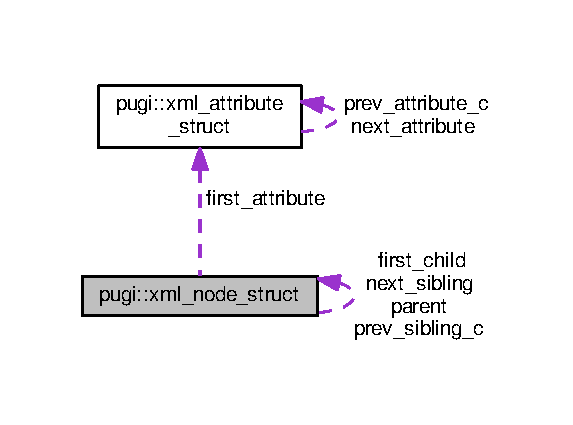
\includegraphics[width=275pt]{structpugi_1_1xml__node__struct__coll__graph}
\end{center}
\end{figure}
\subsection*{Public Member Functions}
\begin{DoxyCompactItemize}
\item 
\hypertarget{structpugi_1_1xml__node__struct_af9af20f835af8b6b99f9a39c93920ea6}{{\bfseries xml\+\_\+node\+\_\+struct} (impl\+::xml\+\_\+memory\+\_\+page $\ast$page, xml\+\_\+node\+\_\+type type)}\label{structpugi_1_1xml__node__struct_af9af20f835af8b6b99f9a39c93920ea6}

\end{DoxyCompactItemize}
\subsection*{Public Attributes}
\begin{DoxyCompactItemize}
\item 
\hypertarget{structpugi_1_1xml__node__struct_aea2e405a368dc5a278a2d23465f1975c}{uintptr\+\_\+t {\bfseries header}}\label{structpugi_1_1xml__node__struct_aea2e405a368dc5a278a2d23465f1975c}

\item 
\hypertarget{structpugi_1_1xml__node__struct_ae2324fdbd1e307fb12007d1d0f957a0b}{char\+\_\+t $\ast$ {\bfseries name}}\label{structpugi_1_1xml__node__struct_ae2324fdbd1e307fb12007d1d0f957a0b}

\item 
\hypertarget{structpugi_1_1xml__node__struct_a191e708864fccda17bb66157afdadd2d}{char\+\_\+t $\ast$ {\bfseries value}}\label{structpugi_1_1xml__node__struct_a191e708864fccda17bb66157afdadd2d}

\item 
\hypertarget{structpugi_1_1xml__node__struct_af692c222bcc5a9f61108cb3ae0b7b5ea}{\hyperlink{structpugi_1_1xml__node__struct}{xml\+\_\+node\+\_\+struct} $\ast$ {\bfseries parent}}\label{structpugi_1_1xml__node__struct_af692c222bcc5a9f61108cb3ae0b7b5ea}

\item 
\hypertarget{structpugi_1_1xml__node__struct_af72c49a0f81928ef664d9d2f0260f23d}{\hyperlink{structpugi_1_1xml__node__struct}{xml\+\_\+node\+\_\+struct} $\ast$ {\bfseries first\+\_\+child}}\label{structpugi_1_1xml__node__struct_af72c49a0f81928ef664d9d2f0260f23d}

\item 
\hypertarget{structpugi_1_1xml__node__struct_a74e62128c88c422c0ed969633bbb2d4e}{\hyperlink{structpugi_1_1xml__node__struct}{xml\+\_\+node\+\_\+struct} $\ast$ {\bfseries prev\+\_\+sibling\+\_\+c}}\label{structpugi_1_1xml__node__struct_a74e62128c88c422c0ed969633bbb2d4e}

\item 
\hypertarget{structpugi_1_1xml__node__struct_acf0867e3a77871e37132046d97398a6d}{\hyperlink{structpugi_1_1xml__node__struct}{xml\+\_\+node\+\_\+struct} $\ast$ {\bfseries next\+\_\+sibling}}\label{structpugi_1_1xml__node__struct_acf0867e3a77871e37132046d97398a6d}

\item 
\hypertarget{structpugi_1_1xml__node__struct_a482d2daf97ce0745661cb2c57d8f6fb3}{\hyperlink{structpugi_1_1xml__attribute__struct}{xml\+\_\+attribute\+\_\+struct} $\ast$ {\bfseries first\+\_\+attribute}}\label{structpugi_1_1xml__node__struct_a482d2daf97ce0745661cb2c57d8f6fb3}

\end{DoxyCompactItemize}


The documentation for this struct was generated from the following file\+:\begin{DoxyCompactItemize}
\item 
resources/pugixml-\/1.\+8/src/pugixml.\+cpp\end{DoxyCompactItemize}

\hypertarget{classpugi_1_1xml__object__range}{\section{pugi\+:\+:xml\+\_\+object\+\_\+range$<$ It $>$ Class Template Reference}
\label{classpugi_1_1xml__object__range}\index{pugi\+::xml\+\_\+object\+\_\+range$<$ It $>$@{pugi\+::xml\+\_\+object\+\_\+range$<$ It $>$}}
}
\subsection*{Public Types}
\begin{DoxyCompactItemize}
\item 
\hypertarget{classpugi_1_1xml__object__range_ace38fcf448c7134e13612f7ce439246c}{typedef It {\bfseries const\+\_\+iterator}}\label{classpugi_1_1xml__object__range_ace38fcf448c7134e13612f7ce439246c}

\item 
\hypertarget{classpugi_1_1xml__object__range_a024ce5292d3b9f2164c1230855fdb501}{typedef It {\bfseries iterator}}\label{classpugi_1_1xml__object__range_a024ce5292d3b9f2164c1230855fdb501}

\end{DoxyCompactItemize}
\subsection*{Public Member Functions}
\begin{DoxyCompactItemize}
\item 
\hypertarget{classpugi_1_1xml__object__range_abf214db65eac081e4478169cb03bce67}{{\bfseries xml\+\_\+object\+\_\+range} (It b, It e)}\label{classpugi_1_1xml__object__range_abf214db65eac081e4478169cb03bce67}

\item 
\hypertarget{classpugi_1_1xml__object__range_ad8d64cefea10330a0f975fbb13a99a8a}{It {\bfseries begin} () const }\label{classpugi_1_1xml__object__range_ad8d64cefea10330a0f975fbb13a99a8a}

\item 
\hypertarget{classpugi_1_1xml__object__range_ad2c9b91aca1c3d4761c767af29a9d7ff}{It {\bfseries end} () const }\label{classpugi_1_1xml__object__range_ad2c9b91aca1c3d4761c767af29a9d7ff}

\end{DoxyCompactItemize}


The documentation for this class was generated from the following file\+:\begin{DoxyCompactItemize}
\item 
resources/pugixml-\/1.\+8/src/pugixml.\+hpp\end{DoxyCompactItemize}

\hypertarget{structpugi_1_1xml__parse__result}{\section{pugi\+:\+:xml\+\_\+parse\+\_\+result Struct Reference}
\label{structpugi_1_1xml__parse__result}\index{pugi\+::xml\+\_\+parse\+\_\+result@{pugi\+::xml\+\_\+parse\+\_\+result}}
}
\subsection*{Public Member Functions}
\begin{DoxyCompactItemize}
\item 
\hypertarget{structpugi_1_1xml__parse__result_a1fd8f66dd233df5f76f63dea8627e589}{{\bfseries operator bool} () const }\label{structpugi_1_1xml__parse__result_a1fd8f66dd233df5f76f63dea8627e589}

\item 
\hypertarget{structpugi_1_1xml__parse__result_add183854c1798f4c8ae74f40def79b03}{const char $\ast$ {\bfseries description} () const }\label{structpugi_1_1xml__parse__result_add183854c1798f4c8ae74f40def79b03}

\end{DoxyCompactItemize}
\subsection*{Public Attributes}
\begin{DoxyCompactItemize}
\item 
\hypertarget{structpugi_1_1xml__parse__result_af8b3e6badea671931017695c8a9dd1af}{xml\+\_\+parse\+\_\+status {\bfseries status}}\label{structpugi_1_1xml__parse__result_af8b3e6badea671931017695c8a9dd1af}

\item 
\hypertarget{structpugi_1_1xml__parse__result_adb61df40459ba6fb1083d22467983086}{ptrdiff\+\_\+t {\bfseries offset}}\label{structpugi_1_1xml__parse__result_adb61df40459ba6fb1083d22467983086}

\item 
\hypertarget{structpugi_1_1xml__parse__result_ad11f279dfce644dfe297e24dc5f72c01}{xml\+\_\+encoding {\bfseries encoding}}\label{structpugi_1_1xml__parse__result_ad11f279dfce644dfe297e24dc5f72c01}

\end{DoxyCompactItemize}


The documentation for this struct was generated from the following files\+:\begin{DoxyCompactItemize}
\item 
resources/pugixml-\/1.\+8/src/pugixml.\+hpp\item 
resources/pugixml-\/1.\+8/src/pugixml.\+cpp\end{DoxyCompactItemize}

\hypertarget{structxml__parser}{\section{xml\+\_\+parser Struct Reference}
\label{structxml__parser}\index{xml\+\_\+parser@{xml\+\_\+parser}}
}


Collaboration diagram for xml\+\_\+parser\+:
\nopagebreak
\begin{figure}[H]
\begin{center}
\leavevmode
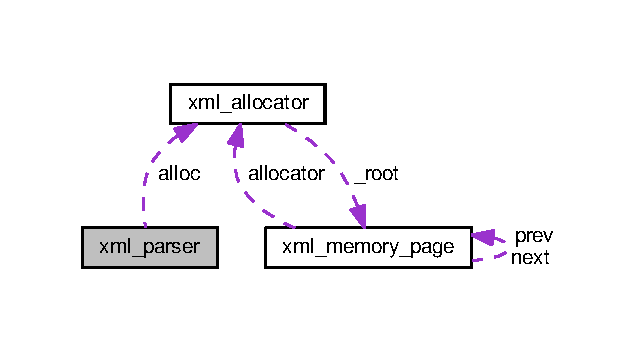
\includegraphics[width=306pt]{structxml__parser__coll__graph}
\end{center}
\end{figure}
\subsection*{Public Member Functions}
\begin{DoxyCompactItemize}
\item 
\hypertarget{structxml__parser_a062d6951738847e674b538a677c8c5f0}{{\bfseries xml\+\_\+parser} (\hyperlink{structxml__allocator}{xml\+\_\+allocator} $\ast$alloc\+\_\+)}\label{structxml__parser_a062d6951738847e674b538a677c8c5f0}

\item 
\hypertarget{structxml__parser_a722853b603ad9a1d1f61bb8115bea5b4}{char\+\_\+t $\ast$ {\bfseries parse\+\_\+doctype\+\_\+primitive} (char\+\_\+t $\ast$s)}\label{structxml__parser_a722853b603ad9a1d1f61bb8115bea5b4}

\item 
\hypertarget{structxml__parser_a1e996ac9c9993f1939128859596376a1}{char\+\_\+t $\ast$ {\bfseries parse\+\_\+doctype\+\_\+ignore} (char\+\_\+t $\ast$s)}\label{structxml__parser_a1e996ac9c9993f1939128859596376a1}

\item 
\hypertarget{structxml__parser_a7804219124faeee80c00a967d16f23e3}{char\+\_\+t $\ast$ {\bfseries parse\+\_\+doctype\+\_\+group} (char\+\_\+t $\ast$s, char\+\_\+t endch)}\label{structxml__parser_a7804219124faeee80c00a967d16f23e3}

\item 
\hypertarget{structxml__parser_a40da52e4b27a0a06752930a0edf16fe9}{char\+\_\+t $\ast$ {\bfseries parse\+\_\+exclamation} (char\+\_\+t $\ast$s, xml\+\_\+node\+\_\+struct $\ast$cursor, unsigned int optmsk, char\+\_\+t endch)}\label{structxml__parser_a40da52e4b27a0a06752930a0edf16fe9}

\item 
\hypertarget{structxml__parser_a2b0edc4fbf2ff448b4d5b31593c5c4fd}{char\+\_\+t $\ast$ {\bfseries parse\+\_\+question} (char\+\_\+t $\ast$s, xml\+\_\+node\+\_\+struct $\ast$\&ref\+\_\+cursor, unsigned int optmsk, char\+\_\+t endch)}\label{structxml__parser_a2b0edc4fbf2ff448b4d5b31593c5c4fd}

\item 
\hypertarget{structxml__parser_a96e76ebea8834b3e56e1c8646e593da4}{char\+\_\+t $\ast$ {\bfseries parse\+\_\+tree} (char\+\_\+t $\ast$s, xml\+\_\+node\+\_\+struct $\ast$root, unsigned int optmsk, char\+\_\+t endch)}\label{structxml__parser_a96e76ebea8834b3e56e1c8646e593da4}

\end{DoxyCompactItemize}
\subsection*{Static Public Member Functions}
\begin{DoxyCompactItemize}
\item 
\hypertarget{structxml__parser_af0a3f5a488b05da9fa2c87e1dd1f9eda}{static char\+\_\+t $\ast$ {\bfseries parse\+\_\+skip\+\_\+bom} (char\+\_\+t $\ast$s)}\label{structxml__parser_af0a3f5a488b05da9fa2c87e1dd1f9eda}

\item 
\hypertarget{structxml__parser_a6be4da5b3206913d0e3bd8320394df41}{static bool {\bfseries has\+\_\+element\+\_\+node\+\_\+siblings} (xml\+\_\+node\+\_\+struct $\ast$node)}\label{structxml__parser_a6be4da5b3206913d0e3bd8320394df41}

\item 
\hypertarget{structxml__parser_a4bf0acd166edf3fc6cc9543002ff6f5d}{static xml\+\_\+parse\+\_\+result {\bfseries parse} (char\+\_\+t $\ast$buffer, size\+\_\+t length, \hyperlink{structxml__document__struct}{xml\+\_\+document\+\_\+struct} $\ast$xmldoc, xml\+\_\+node\+\_\+struct $\ast$root, unsigned int optmsk)}\label{structxml__parser_a4bf0acd166edf3fc6cc9543002ff6f5d}

\end{DoxyCompactItemize}
\subsection*{Public Attributes}
\begin{DoxyCompactItemize}
\item 
\hypertarget{structxml__parser_a48f48b81a9a222b8bcb79f95024faad8}{\hyperlink{structxml__allocator}{xml\+\_\+allocator} $\ast$ {\bfseries alloc}}\label{structxml__parser_a48f48b81a9a222b8bcb79f95024faad8}

\item 
\hypertarget{structxml__parser_a2476a71cd7e67b3f4bdbcd1323524503}{char\+\_\+t $\ast$ {\bfseries error\+\_\+offset}}\label{structxml__parser_a2476a71cd7e67b3f4bdbcd1323524503}

\item 
\hypertarget{structxml__parser_a0555859911674e5a7a349447d6533383}{xml\+\_\+parse\+\_\+status {\bfseries error\+\_\+status}}\label{structxml__parser_a0555859911674e5a7a349447d6533383}

\end{DoxyCompactItemize}


The documentation for this struct was generated from the following file\+:\begin{DoxyCompactItemize}
\item 
resources/pugixml-\/1.\+8/src/pugixml.\+cpp\end{DoxyCompactItemize}

\hypertarget{structxml__stream__chunk}{\section{xml\+\_\+stream\+\_\+chunk$<$ T $>$ Struct Template Reference}
\label{structxml__stream__chunk}\index{xml\+\_\+stream\+\_\+chunk$<$ T $>$@{xml\+\_\+stream\+\_\+chunk$<$ T $>$}}
}


Collaboration diagram for xml\+\_\+stream\+\_\+chunk$<$ T $>$\+:
\nopagebreak
\begin{figure}[H]
\begin{center}
\leavevmode
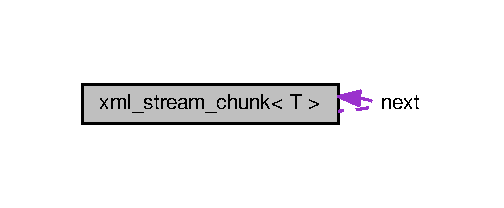
\includegraphics[width=242pt]{structxml__stream__chunk__coll__graph}
\end{center}
\end{figure}
\subsection*{Static Public Member Functions}
\begin{DoxyCompactItemize}
\item 
\hypertarget{structxml__stream__chunk_a92cffe33c529ff266329fd4afb59226d}{static \hyperlink{structxml__stream__chunk}{xml\+\_\+stream\+\_\+chunk} $\ast$ {\bfseries create} ()}\label{structxml__stream__chunk_a92cffe33c529ff266329fd4afb59226d}

\item 
\hypertarget{structxml__stream__chunk_a3e9bf7280c96a7433d60af129873a16f}{static void {\bfseries destroy} (\hyperlink{structxml__stream__chunk}{xml\+\_\+stream\+\_\+chunk} $\ast$chunk)}\label{structxml__stream__chunk_a3e9bf7280c96a7433d60af129873a16f}

\end{DoxyCompactItemize}
\subsection*{Public Attributes}
\begin{DoxyCompactItemize}
\item 
\hypertarget{structxml__stream__chunk_ad00071f7340adb2bde7c4157d4100b3c}{\hyperlink{structxml__stream__chunk}{xml\+\_\+stream\+\_\+chunk} $\ast$ {\bfseries next}}\label{structxml__stream__chunk_ad00071f7340adb2bde7c4157d4100b3c}

\item 
\hypertarget{structxml__stream__chunk_a42618ba3b7bda1246cfc640149fc34eb}{size\+\_\+t {\bfseries size}}\label{structxml__stream__chunk_a42618ba3b7bda1246cfc640149fc34eb}

\item 
\hypertarget{structxml__stream__chunk_a365e2e228a0277467b25a0fea42b8518}{T {\bfseries data} \mbox{[}xml\+\_\+memory\+\_\+page\+\_\+size/sizeof(T)\mbox{]}}\label{structxml__stream__chunk_a365e2e228a0277467b25a0fea42b8518}

\end{DoxyCompactItemize}


The documentation for this struct was generated from the following file\+:\begin{DoxyCompactItemize}
\item 
resources/pugixml-\/1.\+8/src/pugixml.\+cpp\end{DoxyCompactItemize}

\hypertarget{structxml__string__writer}{\section{xml\+\_\+string\+\_\+writer Struct Reference}
\label{structxml__string__writer}\index{xml\+\_\+string\+\_\+writer@{xml\+\_\+string\+\_\+writer}}
}


Inheritance diagram for xml\+\_\+string\+\_\+writer\+:
\nopagebreak
\begin{figure}[H]
\begin{center}
\leavevmode
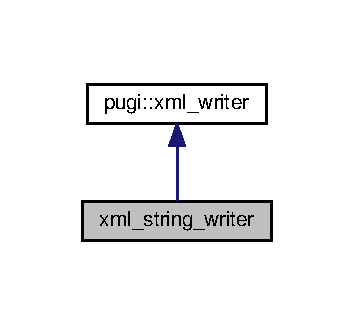
\includegraphics[width=170pt]{structxml__string__writer__inherit__graph}
\end{center}
\end{figure}


Collaboration diagram for xml\+\_\+string\+\_\+writer\+:
\nopagebreak
\begin{figure}[H]
\begin{center}
\leavevmode
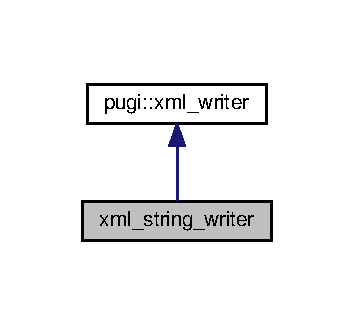
\includegraphics[width=170pt]{structxml__string__writer__coll__graph}
\end{center}
\end{figure}
\subsection*{Public Member Functions}
\begin{DoxyCompactItemize}
\item 
\hypertarget{structxml__string__writer_aa23892a29996648523503b00425f90a2}{virtual void {\bfseries write} (const void $\ast$data, size\+\_\+t size)}\label{structxml__string__writer_aa23892a29996648523503b00425f90a2}

\end{DoxyCompactItemize}
\subsection*{Public Attributes}
\begin{DoxyCompactItemize}
\item 
\hypertarget{structxml__string__writer_a5ffa421ce629a062ca975f5967fef5f7}{std\+::string {\bfseries result}}\label{structxml__string__writer_a5ffa421ce629a062ca975f5967fef5f7}

\end{DoxyCompactItemize}


The documentation for this struct was generated from the following file\+:\begin{DoxyCompactItemize}
\item 
resources/pugixml-\/1.\+8/docs/samples/save\+\_\+custom\+\_\+writer.\+cpp\end{DoxyCompactItemize}

\hypertarget{classpugi_1_1xml__text}{\section{pugi\+:\+:xml\+\_\+text Class Reference}
\label{classpugi_1_1xml__text}\index{pugi\+::xml\+\_\+text@{pugi\+::xml\+\_\+text}}
}
\subsection*{Public Member Functions}
\begin{DoxyCompactItemize}
\item 
\hypertarget{classpugi_1_1xml__text_a549820a92ece6ed347f721d7676822e5}{{\bfseries operator unspecified\+\_\+bool\+\_\+type} () const }\label{classpugi_1_1xml__text_a549820a92ece6ed347f721d7676822e5}

\item 
\hypertarget{classpugi_1_1xml__text_ab75d176a3c799a4638ac298390dbed4c}{bool {\bfseries operator!} () const }\label{classpugi_1_1xml__text_ab75d176a3c799a4638ac298390dbed4c}

\item 
\hypertarget{classpugi_1_1xml__text_a673a7eac0048e7bcdfd32ee6a5820798}{bool {\bfseries empty} () const }\label{classpugi_1_1xml__text_a673a7eac0048e7bcdfd32ee6a5820798}

\item 
\hypertarget{classpugi_1_1xml__text_acf75854306f4756904b6ef140ba1b53f}{const char\+\_\+t $\ast$ {\bfseries get} () const }\label{classpugi_1_1xml__text_acf75854306f4756904b6ef140ba1b53f}

\item 
\hypertarget{classpugi_1_1xml__text_ac817e480d7ab09b3c6390622423a701b}{const char\+\_\+t $\ast$ {\bfseries as\+\_\+string} (const char\+\_\+t $\ast$def=P\+U\+G\+I\+X\+M\+L\+\_\+\+T\+E\+X\+T(\char`\"{}\char`\"{})) const }\label{classpugi_1_1xml__text_ac817e480d7ab09b3c6390622423a701b}

\item 
\hypertarget{classpugi_1_1xml__text_a71d4c7ed3d12dc6e8ee2a81d293fe9f4}{int {\bfseries as\+\_\+int} (int def=0) const }\label{classpugi_1_1xml__text_a71d4c7ed3d12dc6e8ee2a81d293fe9f4}

\item 
\hypertarget{classpugi_1_1xml__text_a9eb828629c4ca107d06d28a60f5bb114}{unsigned int {\bfseries as\+\_\+uint} (unsigned int def=0) const }\label{classpugi_1_1xml__text_a9eb828629c4ca107d06d28a60f5bb114}

\item 
\hypertarget{classpugi_1_1xml__text_aa6722fcf1c4e10ee11b6df73bef11cee}{double {\bfseries as\+\_\+double} (double def=0) const }\label{classpugi_1_1xml__text_aa6722fcf1c4e10ee11b6df73bef11cee}

\item 
\hypertarget{classpugi_1_1xml__text_a158482df06cd778542d7cedb1c33e39f}{float {\bfseries as\+\_\+float} (float def=0) const }\label{classpugi_1_1xml__text_a158482df06cd778542d7cedb1c33e39f}

\item 
\hypertarget{classpugi_1_1xml__text_ab591c10f3adc62024cf8ffc53c4e372e}{bool {\bfseries as\+\_\+bool} (bool def=false) const }\label{classpugi_1_1xml__text_ab591c10f3adc62024cf8ffc53c4e372e}

\item 
\hypertarget{classpugi_1_1xml__text_ab31930ff4f5ad568549f85dbb697e60e}{bool {\bfseries set} (const char\+\_\+t $\ast$rhs)}\label{classpugi_1_1xml__text_ab31930ff4f5ad568549f85dbb697e60e}

\item 
\hypertarget{classpugi_1_1xml__text_a66ebe5bd62e843197305ed68661b0a26}{bool {\bfseries set} (int rhs)}\label{classpugi_1_1xml__text_a66ebe5bd62e843197305ed68661b0a26}

\item 
\hypertarget{classpugi_1_1xml__text_a9d780e113aa0b1f4bbf2d0a88fe2c42f}{bool {\bfseries set} (unsigned int rhs)}\label{classpugi_1_1xml__text_a9d780e113aa0b1f4bbf2d0a88fe2c42f}

\item 
\hypertarget{classpugi_1_1xml__text_a998d885909d8bb43c40f03cd27e1c809}{bool {\bfseries set} (long rhs)}\label{classpugi_1_1xml__text_a998d885909d8bb43c40f03cd27e1c809}

\item 
\hypertarget{classpugi_1_1xml__text_a19d022a9aa6734d10f05a47862234e90}{bool {\bfseries set} (unsigned long rhs)}\label{classpugi_1_1xml__text_a19d022a9aa6734d10f05a47862234e90}

\item 
\hypertarget{classpugi_1_1xml__text_acf32e49c31a07f7bad1f9bdfb71bdc1e}{bool {\bfseries set} (double rhs)}\label{classpugi_1_1xml__text_acf32e49c31a07f7bad1f9bdfb71bdc1e}

\item 
\hypertarget{classpugi_1_1xml__text_a5de352282b5673bf5c98d22831f946a7}{bool {\bfseries set} (float rhs)}\label{classpugi_1_1xml__text_a5de352282b5673bf5c98d22831f946a7}

\item 
\hypertarget{classpugi_1_1xml__text_a0d75ccc7ede3b3d590352267a0f0fcb9}{bool {\bfseries set} (bool rhs)}\label{classpugi_1_1xml__text_a0d75ccc7ede3b3d590352267a0f0fcb9}

\item 
\hypertarget{classpugi_1_1xml__text_a0b895996d14f50afca11b9a82276038d}{\hyperlink{classpugi_1_1xml__text}{xml\+\_\+text} \& {\bfseries operator=} (const char\+\_\+t $\ast$rhs)}\label{classpugi_1_1xml__text_a0b895996d14f50afca11b9a82276038d}

\item 
\hypertarget{classpugi_1_1xml__text_a594653404f095b07d4644a0567f9ec51}{\hyperlink{classpugi_1_1xml__text}{xml\+\_\+text} \& {\bfseries operator=} (int rhs)}\label{classpugi_1_1xml__text_a594653404f095b07d4644a0567f9ec51}

\item 
\hypertarget{classpugi_1_1xml__text_a48e2aa3796629258d1f037d1bc2277f7}{\hyperlink{classpugi_1_1xml__text}{xml\+\_\+text} \& {\bfseries operator=} (unsigned int rhs)}\label{classpugi_1_1xml__text_a48e2aa3796629258d1f037d1bc2277f7}

\item 
\hypertarget{classpugi_1_1xml__text_aafebcd3794846d78578bee6feeaefbaf}{\hyperlink{classpugi_1_1xml__text}{xml\+\_\+text} \& {\bfseries operator=} (long rhs)}\label{classpugi_1_1xml__text_aafebcd3794846d78578bee6feeaefbaf}

\item 
\hypertarget{classpugi_1_1xml__text_ad5bd2426b8a4294f156d1dd129a636d1}{\hyperlink{classpugi_1_1xml__text}{xml\+\_\+text} \& {\bfseries operator=} (unsigned long rhs)}\label{classpugi_1_1xml__text_ad5bd2426b8a4294f156d1dd129a636d1}

\item 
\hypertarget{classpugi_1_1xml__text_a0ff3e37177494d9cdfa073c6392ca405}{\hyperlink{classpugi_1_1xml__text}{xml\+\_\+text} \& {\bfseries operator=} (double rhs)}\label{classpugi_1_1xml__text_a0ff3e37177494d9cdfa073c6392ca405}

\item 
\hypertarget{classpugi_1_1xml__text_ab2ef884aa761a5ef96eb643a11c6734a}{\hyperlink{classpugi_1_1xml__text}{xml\+\_\+text} \& {\bfseries operator=} (float rhs)}\label{classpugi_1_1xml__text_ab2ef884aa761a5ef96eb643a11c6734a}

\item 
\hypertarget{classpugi_1_1xml__text_afd64e76239853fcf57e80b8f43a3fb4d}{\hyperlink{classpugi_1_1xml__text}{xml\+\_\+text} \& {\bfseries operator=} (bool rhs)}\label{classpugi_1_1xml__text_afd64e76239853fcf57e80b8f43a3fb4d}

\item 
\hypertarget{classpugi_1_1xml__text_a30ca257f1614159c625d2904a6285224}{\hyperlink{classpugi_1_1xml__node}{xml\+\_\+node} {\bfseries data} () const }\label{classpugi_1_1xml__text_a30ca257f1614159c625d2904a6285224}

\end{DoxyCompactItemize}
\subsection*{Friends}
\begin{DoxyCompactItemize}
\item 
\hypertarget{classpugi_1_1xml__text_a156d917a92815c7b593bd5ef19f6d5fb}{class {\bfseries xml\+\_\+node}}\label{classpugi_1_1xml__text_a156d917a92815c7b593bd5ef19f6d5fb}

\end{DoxyCompactItemize}


The documentation for this class was generated from the following files\+:\begin{DoxyCompactItemize}
\item 
resources/pugixml-\/1.\+8/src/pugixml.\+hpp\item 
resources/pugixml-\/1.\+8/src/pugixml.\+cpp\end{DoxyCompactItemize}

\hypertarget{classpugi_1_1xml__tree__walker}{\section{pugi\+:\+:xml\+\_\+tree\+\_\+walker Class Reference}
\label{classpugi_1_1xml__tree__walker}\index{pugi\+::xml\+\_\+tree\+\_\+walker@{pugi\+::xml\+\_\+tree\+\_\+walker}}
}


Inheritance diagram for pugi\+:\+:xml\+\_\+tree\+\_\+walker\+:
\nopagebreak
\begin{figure}[H]
\begin{center}
\leavevmode
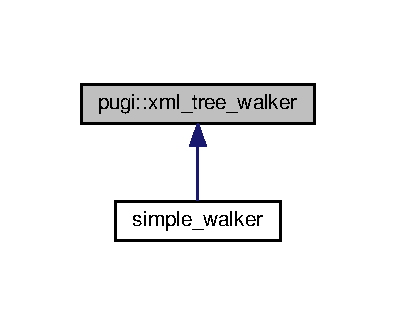
\includegraphics[width=190pt]{classpugi_1_1xml__tree__walker__inherit__graph}
\end{center}
\end{figure}
\subsection*{Public Member Functions}
\begin{DoxyCompactItemize}
\item 
\hypertarget{classpugi_1_1xml__tree__walker_a831cc2fc61a47e23673c85efc41bc7a2}{virtual bool {\bfseries begin} (\hyperlink{classpugi_1_1xml__node}{xml\+\_\+node} \&node)}\label{classpugi_1_1xml__tree__walker_a831cc2fc61a47e23673c85efc41bc7a2}

\item 
\hypertarget{classpugi_1_1xml__tree__walker_a309363c9d17ef3fc8cacc6f71fcbea88}{virtual bool {\bfseries for\+\_\+each} (\hyperlink{classpugi_1_1xml__node}{xml\+\_\+node} \&node)=0}\label{classpugi_1_1xml__tree__walker_a309363c9d17ef3fc8cacc6f71fcbea88}

\item 
\hypertarget{classpugi_1_1xml__tree__walker_a24e6ffd4a8351e2ee486440b6f784091}{virtual bool {\bfseries end} (\hyperlink{classpugi_1_1xml__node}{xml\+\_\+node} \&node)}\label{classpugi_1_1xml__tree__walker_a24e6ffd4a8351e2ee486440b6f784091}

\end{DoxyCompactItemize}
\subsection*{Protected Member Functions}
\begin{DoxyCompactItemize}
\item 
\hypertarget{classpugi_1_1xml__tree__walker_acb27ca9fea177b0741f29274cb0c805a}{int {\bfseries depth} () const }\label{classpugi_1_1xml__tree__walker_acb27ca9fea177b0741f29274cb0c805a}

\end{DoxyCompactItemize}
\subsection*{Friends}
\begin{DoxyCompactItemize}
\item 
\hypertarget{classpugi_1_1xml__tree__walker_a156d917a92815c7b593bd5ef19f6d5fb}{class {\bfseries xml\+\_\+node}}\label{classpugi_1_1xml__tree__walker_a156d917a92815c7b593bd5ef19f6d5fb}

\end{DoxyCompactItemize}


The documentation for this class was generated from the following files\+:\begin{DoxyCompactItemize}
\item 
resources/pugixml-\/1.\+8/src/pugixml.\+hpp\item 
resources/pugixml-\/1.\+8/src/pugixml.\+cpp\end{DoxyCompactItemize}

\hypertarget{classpugi_1_1xml__writer}{\section{pugi\+:\+:xml\+\_\+writer Class Reference}
\label{classpugi_1_1xml__writer}\index{pugi\+::xml\+\_\+writer@{pugi\+::xml\+\_\+writer}}
}


Inheritance diagram for pugi\+:\+:xml\+\_\+writer\+:
\nopagebreak
\begin{figure}[H]
\begin{center}
\leavevmode
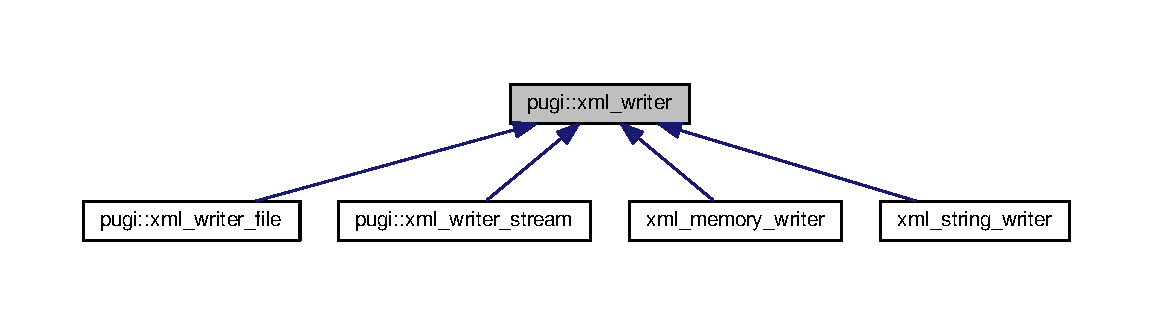
\includegraphics[width=350pt]{classpugi_1_1xml__writer__inherit__graph}
\end{center}
\end{figure}
\subsection*{Public Member Functions}
\begin{DoxyCompactItemize}
\item 
\hypertarget{classpugi_1_1xml__writer_ab7d3b6a8499ceef7799158370e1c2617}{virtual void {\bfseries write} (const void $\ast$data, size\+\_\+t size)=0}\label{classpugi_1_1xml__writer_ab7d3b6a8499ceef7799158370e1c2617}

\end{DoxyCompactItemize}


The documentation for this class was generated from the following file\+:\begin{DoxyCompactItemize}
\item 
resources/pugixml-\/1.\+8/src/pugixml.\+hpp\end{DoxyCompactItemize}

\hypertarget{classpugi_1_1xml__writer__file}{\section{pugi\+:\+:xml\+\_\+writer\+\_\+file Class Reference}
\label{classpugi_1_1xml__writer__file}\index{pugi\+::xml\+\_\+writer\+\_\+file@{pugi\+::xml\+\_\+writer\+\_\+file}}
}


Inheritance diagram for pugi\+:\+:xml\+\_\+writer\+\_\+file\+:
\nopagebreak
\begin{figure}[H]
\begin{center}
\leavevmode
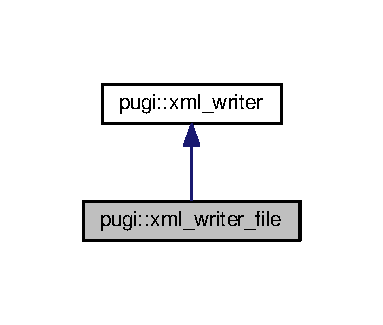
\includegraphics[width=184pt]{classpugi_1_1xml__writer__file__inherit__graph}
\end{center}
\end{figure}


Collaboration diagram for pugi\+:\+:xml\+\_\+writer\+\_\+file\+:
\nopagebreak
\begin{figure}[H]
\begin{center}
\leavevmode
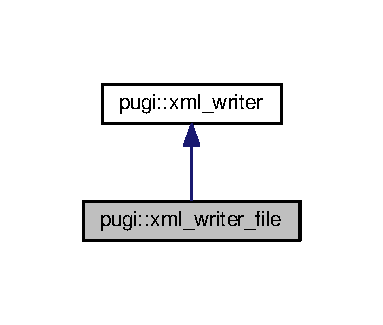
\includegraphics[width=184pt]{classpugi_1_1xml__writer__file__coll__graph}
\end{center}
\end{figure}
\subsection*{Public Member Functions}
\begin{DoxyCompactItemize}
\item 
\hypertarget{classpugi_1_1xml__writer__file_a458afaf5231f88e182fa16b13fc2b0a6}{{\bfseries xml\+\_\+writer\+\_\+file} (void $\ast$file)}\label{classpugi_1_1xml__writer__file_a458afaf5231f88e182fa16b13fc2b0a6}

\item 
\hypertarget{classpugi_1_1xml__writer__file_af89c557be2a43f11836f1f4db50855e6}{virtual void {\bfseries write} (const void $\ast$data, size\+\_\+t size) P\+U\+G\+I\+X\+M\+L\+\_\+\+O\+V\+E\+R\+R\+I\+D\+E}\label{classpugi_1_1xml__writer__file_af89c557be2a43f11836f1f4db50855e6}

\end{DoxyCompactItemize}


The documentation for this class was generated from the following files\+:\begin{DoxyCompactItemize}
\item 
resources/pugixml-\/1.\+8/src/pugixml.\+hpp\item 
resources/pugixml-\/1.\+8/src/pugixml.\+cpp\end{DoxyCompactItemize}

\hypertarget{classpugi_1_1xml__writer__stream}{\section{pugi\+:\+:xml\+\_\+writer\+\_\+stream Class Reference}
\label{classpugi_1_1xml__writer__stream}\index{pugi\+::xml\+\_\+writer\+\_\+stream@{pugi\+::xml\+\_\+writer\+\_\+stream}}
}


Inheritance diagram for pugi\+:\+:xml\+\_\+writer\+\_\+stream\+:
\nopagebreak
\begin{figure}[H]
\begin{center}
\leavevmode
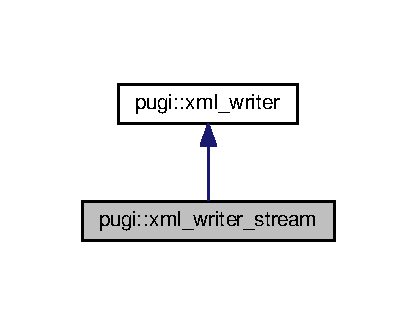
\includegraphics[width=200pt]{classpugi_1_1xml__writer__stream__inherit__graph}
\end{center}
\end{figure}


Collaboration diagram for pugi\+:\+:xml\+\_\+writer\+\_\+stream\+:
\nopagebreak
\begin{figure}[H]
\begin{center}
\leavevmode
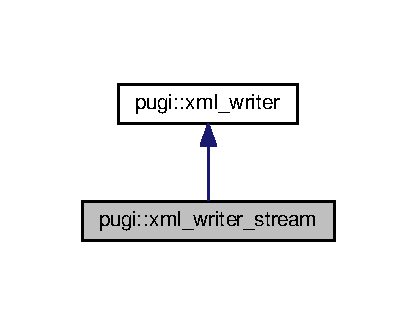
\includegraphics[width=200pt]{classpugi_1_1xml__writer__stream__coll__graph}
\end{center}
\end{figure}
\subsection*{Public Member Functions}
\begin{DoxyCompactItemize}
\item 
\hypertarget{classpugi_1_1xml__writer__stream_a259c28368c08378e15cf28b35a1dcd9a}{{\bfseries xml\+\_\+writer\+\_\+stream} (std\+::basic\+\_\+ostream$<$ char, std\+::char\+\_\+traits$<$ char $>$ $>$ \&stream)}\label{classpugi_1_1xml__writer__stream_a259c28368c08378e15cf28b35a1dcd9a}

\item 
\hypertarget{classpugi_1_1xml__writer__stream_afa342cf0bb3a0bd6ee3d47550ad23333}{{\bfseries xml\+\_\+writer\+\_\+stream} (std\+::basic\+\_\+ostream$<$ wchar\+\_\+t, std\+::char\+\_\+traits$<$ wchar\+\_\+t $>$ $>$ \&stream)}\label{classpugi_1_1xml__writer__stream_afa342cf0bb3a0bd6ee3d47550ad23333}

\item 
\hypertarget{classpugi_1_1xml__writer__stream_a331839df873b20fd6d32b25f3eeb5856}{virtual void {\bfseries write} (const void $\ast$data, size\+\_\+t size) P\+U\+G\+I\+X\+M\+L\+\_\+\+O\+V\+E\+R\+R\+I\+D\+E}\label{classpugi_1_1xml__writer__stream_a331839df873b20fd6d32b25f3eeb5856}

\end{DoxyCompactItemize}


The documentation for this class was generated from the following files\+:\begin{DoxyCompactItemize}
\item 
resources/pugixml-\/1.\+8/src/pugixml.\+hpp\item 
resources/pugixml-\/1.\+8/src/pugixml.\+cpp\end{DoxyCompactItemize}

\hypertarget{classxpath__allocator}{\section{xpath\+\_\+allocator Class Reference}
\label{classxpath__allocator}\index{xpath\+\_\+allocator@{xpath\+\_\+allocator}}
}
\subsection*{Public Member Functions}
\begin{DoxyCompactItemize}
\item 
\hypertarget{classxpath__allocator_a3b8ba1722fba115d05949d8f592080e8}{{\bfseries xpath\+\_\+allocator} (\hyperlink{structxpath__memory__block}{xpath\+\_\+memory\+\_\+block} $\ast$root, size\+\_\+t root\+\_\+size=0)}\label{classxpath__allocator_a3b8ba1722fba115d05949d8f592080e8}

\item 
\hypertarget{classxpath__allocator_aa66f3703548657eca5316392a2d79d00}{void $\ast$ {\bfseries allocate\+\_\+nothrow} (size\+\_\+t size)}\label{classxpath__allocator_aa66f3703548657eca5316392a2d79d00}

\item 
\hypertarget{classxpath__allocator_aad95aa445f2fdc7c3d1c19b1f3d67cb1}{void $\ast$ {\bfseries allocate} (size\+\_\+t size)}\label{classxpath__allocator_aad95aa445f2fdc7c3d1c19b1f3d67cb1}

\item 
\hypertarget{classxpath__allocator_a4dd502389202ec8e7420832112a571e5}{void $\ast$ {\bfseries reallocate} (void $\ast$ptr, size\+\_\+t old\+\_\+size, size\+\_\+t new\+\_\+size)}\label{classxpath__allocator_a4dd502389202ec8e7420832112a571e5}

\item 
\hypertarget{classxpath__allocator_af1c3ec117935d4488bbd16adf807fbc1}{void {\bfseries revert} (const \hyperlink{classxpath__allocator}{xpath\+\_\+allocator} \&state)}\label{classxpath__allocator_af1c3ec117935d4488bbd16adf807fbc1}

\item 
\hypertarget{classxpath__allocator_a9436b8bdef3e0e0ff0df28c2af6a430d}{void {\bfseries release} ()}\label{classxpath__allocator_a9436b8bdef3e0e0ff0df28c2af6a430d}

\end{DoxyCompactItemize}


The documentation for this class was generated from the following file\+:\begin{DoxyCompactItemize}
\item 
resources/pugixml-\/1.\+8/src/pugixml.\+cpp\end{DoxyCompactItemize}

\hypertarget{structxpath__allocator__capture}{\section{xpath\+\_\+allocator\+\_\+capture Struct Reference}
\label{structxpath__allocator__capture}\index{xpath\+\_\+allocator\+\_\+capture@{xpath\+\_\+allocator\+\_\+capture}}
}


Collaboration diagram for xpath\+\_\+allocator\+\_\+capture\+:
\nopagebreak
\begin{figure}[H]
\begin{center}
\leavevmode
\includegraphics[width=198pt]{structxpath__allocator__capture__coll__graph}
\end{center}
\end{figure}
\subsection*{Public Member Functions}
\begin{DoxyCompactItemize}
\item 
\hypertarget{structxpath__allocator__capture_af6925e08c811c0cbda74d4da5b9f2eed}{{\bfseries xpath\+\_\+allocator\+\_\+capture} (\hyperlink{classxpath__allocator}{xpath\+\_\+allocator} $\ast$alloc)}\label{structxpath__allocator__capture_af6925e08c811c0cbda74d4da5b9f2eed}

\end{DoxyCompactItemize}
\subsection*{Public Attributes}
\begin{DoxyCompactItemize}
\item 
\hypertarget{structxpath__allocator__capture_a382acca931c691699ec84a03fb060cf4}{\hyperlink{classxpath__allocator}{xpath\+\_\+allocator} $\ast$ {\bfseries \+\_\+target}}\label{structxpath__allocator__capture_a382acca931c691699ec84a03fb060cf4}

\item 
\hypertarget{structxpath__allocator__capture_a275859dc99681c12b42ee4f51b713d39}{\hyperlink{classxpath__allocator}{xpath\+\_\+allocator} {\bfseries \+\_\+state}}\label{structxpath__allocator__capture_a275859dc99681c12b42ee4f51b713d39}

\end{DoxyCompactItemize}


The documentation for this struct was generated from the following file\+:\begin{DoxyCompactItemize}
\item 
resources/pugixml-\/1.\+8/src/pugixml.\+cpp\end{DoxyCompactItemize}

\hypertarget{classxpath__ast__node}{\section{xpath\+\_\+ast\+\_\+node Class Reference}
\label{classxpath__ast__node}\index{xpath\+\_\+ast\+\_\+node@{xpath\+\_\+ast\+\_\+node}}
}
\subsection*{Public Member Functions}
\begin{DoxyCompactItemize}
\item 
\hypertarget{classxpath__ast__node_af155d17a4477a693d37f4e34957dcc21}{{\bfseries xpath\+\_\+ast\+\_\+node} (ast\+\_\+type\+\_\+t type, xpath\+\_\+value\+\_\+type rettype\+\_\+, const char\+\_\+t $\ast$value)}\label{classxpath__ast__node_af155d17a4477a693d37f4e34957dcc21}

\item 
\hypertarget{classxpath__ast__node_ada97458f3fc7d6c87cf70d8084117b0d}{{\bfseries xpath\+\_\+ast\+\_\+node} (ast\+\_\+type\+\_\+t type, xpath\+\_\+value\+\_\+type rettype\+\_\+, double value)}\label{classxpath__ast__node_ada97458f3fc7d6c87cf70d8084117b0d}

\item 
\hypertarget{classxpath__ast__node_a8de4244f7b9fc7626049197ddc0afab7}{{\bfseries xpath\+\_\+ast\+\_\+node} (ast\+\_\+type\+\_\+t type, xpath\+\_\+value\+\_\+type rettype\+\_\+, xpath\+\_\+variable $\ast$value)}\label{classxpath__ast__node_a8de4244f7b9fc7626049197ddc0afab7}

\item 
\hypertarget{classxpath__ast__node_af6f4ffea3f3c7fdb6ef1e759d4b070f4}{{\bfseries xpath\+\_\+ast\+\_\+node} (ast\+\_\+type\+\_\+t type, xpath\+\_\+value\+\_\+type rettype\+\_\+, \hyperlink{classxpath__ast__node}{xpath\+\_\+ast\+\_\+node} $\ast$left=0, \hyperlink{classxpath__ast__node}{xpath\+\_\+ast\+\_\+node} $\ast$right=0)}\label{classxpath__ast__node_af6f4ffea3f3c7fdb6ef1e759d4b070f4}

\item 
\hypertarget{classxpath__ast__node_a7cf74b277deba86a6575796c727fe458}{{\bfseries xpath\+\_\+ast\+\_\+node} (ast\+\_\+type\+\_\+t type, \hyperlink{classxpath__ast__node}{xpath\+\_\+ast\+\_\+node} $\ast$left, axis\+\_\+t axis, nodetest\+\_\+t test, const char\+\_\+t $\ast$contents)}\label{classxpath__ast__node_a7cf74b277deba86a6575796c727fe458}

\item 
\hypertarget{classxpath__ast__node_aef76c6d41da27404909e62437fc9f02c}{{\bfseries xpath\+\_\+ast\+\_\+node} (ast\+\_\+type\+\_\+t type, \hyperlink{classxpath__ast__node}{xpath\+\_\+ast\+\_\+node} $\ast$left, \hyperlink{classxpath__ast__node}{xpath\+\_\+ast\+\_\+node} $\ast$right, predicate\+\_\+t test)}\label{classxpath__ast__node_aef76c6d41da27404909e62437fc9f02c}

\item 
\hypertarget{classxpath__ast__node_a2764184d076834284eb3ff3182b845cc}{void {\bfseries set\+\_\+next} (\hyperlink{classxpath__ast__node}{xpath\+\_\+ast\+\_\+node} $\ast$value)}\label{classxpath__ast__node_a2764184d076834284eb3ff3182b845cc}

\item 
\hypertarget{classxpath__ast__node_afe044146db852b7d4dbf188fd2ff6c75}{void {\bfseries set\+\_\+right} (\hyperlink{classxpath__ast__node}{xpath\+\_\+ast\+\_\+node} $\ast$value)}\label{classxpath__ast__node_afe044146db852b7d4dbf188fd2ff6c75}

\item 
\hypertarget{classxpath__ast__node_ab7f965a92023bc2704b8e6fd9f3d7c14}{bool {\bfseries eval\+\_\+boolean} (const \hyperlink{structxpath__context}{xpath\+\_\+context} \&c, const \hyperlink{structxpath__stack}{xpath\+\_\+stack} \&stack)}\label{classxpath__ast__node_ab7f965a92023bc2704b8e6fd9f3d7c14}

\item 
\hypertarget{classxpath__ast__node_a92dd7048e28d486bc7f382d1fc6f1de6}{double {\bfseries eval\+\_\+number} (const \hyperlink{structxpath__context}{xpath\+\_\+context} \&c, const \hyperlink{structxpath__stack}{xpath\+\_\+stack} \&stack)}\label{classxpath__ast__node_a92dd7048e28d486bc7f382d1fc6f1de6}

\item 
\hypertarget{classxpath__ast__node_aaf931a091af0fb91c25e90b205363b4e}{\hyperlink{classxpath__string}{xpath\+\_\+string} {\bfseries eval\+\_\+string\+\_\+concat} (const \hyperlink{structxpath__context}{xpath\+\_\+context} \&c, const \hyperlink{structxpath__stack}{xpath\+\_\+stack} \&stack)}\label{classxpath__ast__node_aaf931a091af0fb91c25e90b205363b4e}

\item 
\hypertarget{classxpath__ast__node_a6b675237a590548b68d0e0b97518b6df}{\hyperlink{classxpath__string}{xpath\+\_\+string} {\bfseries eval\+\_\+string} (const \hyperlink{structxpath__context}{xpath\+\_\+context} \&c, const \hyperlink{structxpath__stack}{xpath\+\_\+stack} \&stack)}\label{classxpath__ast__node_a6b675237a590548b68d0e0b97518b6df}

\item 
\hypertarget{classxpath__ast__node_a68cace396dd4eeae67ecfcd34a3a8285}{\hyperlink{classxpath__node__set__raw}{xpath\+\_\+node\+\_\+set\+\_\+raw} {\bfseries eval\+\_\+node\+\_\+set} (const \hyperlink{structxpath__context}{xpath\+\_\+context} \&c, const \hyperlink{structxpath__stack}{xpath\+\_\+stack} \&stack, nodeset\+\_\+eval\+\_\+t eval)}\label{classxpath__ast__node_a68cace396dd4eeae67ecfcd34a3a8285}

\item 
\hypertarget{classxpath__ast__node_a950534fc7de08fe40d897ebea84c1d6d}{void {\bfseries optimize} (\hyperlink{classxpath__allocator}{xpath\+\_\+allocator} $\ast$alloc)}\label{classxpath__ast__node_a950534fc7de08fe40d897ebea84c1d6d}

\item 
\hypertarget{classxpath__ast__node_a3eb089927cabd867a3a9d1b723aece0d}{void {\bfseries optimize\+\_\+self} (\hyperlink{classxpath__allocator}{xpath\+\_\+allocator} $\ast$alloc)}\label{classxpath__ast__node_a3eb089927cabd867a3a9d1b723aece0d}

\item 
\hypertarget{classxpath__ast__node_aa683d40f3ad22dfe89889bf6ca888082}{bool {\bfseries is\+\_\+posinv\+\_\+expr} () const }\label{classxpath__ast__node_aa683d40f3ad22dfe89889bf6ca888082}

\item 
\hypertarget{classxpath__ast__node_a2af0b84caf47031c30c80f5c2206392e}{bool {\bfseries is\+\_\+posinv\+\_\+step} () const }\label{classxpath__ast__node_a2af0b84caf47031c30c80f5c2206392e}

\item 
\hypertarget{classxpath__ast__node_a2c3598521141ed4b763fe6c4f852234f}{xpath\+\_\+value\+\_\+type {\bfseries rettype} () const }\label{classxpath__ast__node_a2c3598521141ed4b763fe6c4f852234f}

\end{DoxyCompactItemize}


The documentation for this class was generated from the following file\+:\begin{DoxyCompactItemize}
\item 
resources/pugixml-\/1.\+8/src/pugixml.\+cpp\end{DoxyCompactItemize}

\hypertarget{structxpath__context}{\section{xpath\+\_\+context Struct Reference}
\label{structxpath__context}\index{xpath\+\_\+context@{xpath\+\_\+context}}
}
\subsection*{Public Member Functions}
\begin{DoxyCompactItemize}
\item 
\hypertarget{structxpath__context_ab5d7a8d5a14ef695b93e15cfb0e20386}{{\bfseries xpath\+\_\+context} (const xpath\+\_\+node \&n\+\_\+, size\+\_\+t position\+\_\+, size\+\_\+t size\+\_\+)}\label{structxpath__context_ab5d7a8d5a14ef695b93e15cfb0e20386}

\end{DoxyCompactItemize}
\subsection*{Public Attributes}
\begin{DoxyCompactItemize}
\item 
\hypertarget{structxpath__context_ace8fbb8121820bc5054605c166101273}{xpath\+\_\+node {\bfseries n}}\label{structxpath__context_ace8fbb8121820bc5054605c166101273}

\item 
\hypertarget{structxpath__context_add1fc9bd16b21d3a8d7a4bd63c60af07}{size\+\_\+t {\bfseries position}}\label{structxpath__context_add1fc9bd16b21d3a8d7a4bd63c60af07}

\item 
\hypertarget{structxpath__context_a976ffb0eff84a7779c97e589c1785d1c}{size\+\_\+t {\bfseries size}}\label{structxpath__context_a976ffb0eff84a7779c97e589c1785d1c}

\end{DoxyCompactItemize}


The documentation for this struct was generated from the following file\+:\begin{DoxyCompactItemize}
\item 
resources/pugixml-\/1.\+8/src/pugixml.\+cpp\end{DoxyCompactItemize}

\hypertarget{classpugi_1_1xpath__exception}{\section{pugi\+:\+:xpath\+\_\+exception Class Reference}
\label{classpugi_1_1xpath__exception}\index{pugi\+::xpath\+\_\+exception@{pugi\+::xpath\+\_\+exception}}
}


Inheritance diagram for pugi\+:\+:xpath\+\_\+exception\+:
\nopagebreak
\begin{figure}[H]
\begin{center}
\leavevmode
\includegraphics[width=190pt]{classpugi_1_1xpath__exception__inherit__graph}
\end{center}
\end{figure}


Collaboration diagram for pugi\+:\+:xpath\+\_\+exception\+:
\nopagebreak
\begin{figure}[H]
\begin{center}
\leavevmode
\includegraphics[width=190pt]{classpugi_1_1xpath__exception__coll__graph}
\end{center}
\end{figure}
\subsection*{Public Member Functions}
\begin{DoxyCompactItemize}
\item 
\hypertarget{classpugi_1_1xpath__exception_a67698821481b5a73213d21a1ac174410}{{\bfseries xpath\+\_\+exception} (const \hyperlink{structpugi_1_1xpath__parse__result}{xpath\+\_\+parse\+\_\+result} \&result)}\label{classpugi_1_1xpath__exception_a67698821481b5a73213d21a1ac174410}

\item 
\hypertarget{classpugi_1_1xpath__exception_a3451312335446d093e4e5382dc18bd27}{virtual const char $\ast$ {\bfseries what} () const P\+U\+G\+I\+X\+M\+L\+\_\+\+O\+V\+E\+R\+R\+I\+D\+E  throw ()}\label{classpugi_1_1xpath__exception_a3451312335446d093e4e5382dc18bd27}

\item 
\hypertarget{classpugi_1_1xpath__exception_a6602bbd541153f35a44c2233aa7d37de}{const \hyperlink{structpugi_1_1xpath__parse__result}{xpath\+\_\+parse\+\_\+result} \& {\bfseries result} () const }\label{classpugi_1_1xpath__exception_a6602bbd541153f35a44c2233aa7d37de}

\end{DoxyCompactItemize}


The documentation for this class was generated from the following files\+:\begin{DoxyCompactItemize}
\item 
resources/pugixml-\/1.\+8/src/pugixml.\+hpp\item 
resources/pugixml-\/1.\+8/src/pugixml.\+cpp\end{DoxyCompactItemize}

\hypertarget{classxpath__lexer}{\section{xpath\+\_\+lexer Class Reference}
\label{classxpath__lexer}\index{xpath\+\_\+lexer@{xpath\+\_\+lexer}}
}
\subsection*{Public Member Functions}
\begin{DoxyCompactItemize}
\item 
\hypertarget{classxpath__lexer_aa52661c9ba7dfa262d3ab49f578653c3}{{\bfseries xpath\+\_\+lexer} (const char\+\_\+t $\ast$query)}\label{classxpath__lexer_aa52661c9ba7dfa262d3ab49f578653c3}

\item 
\hypertarget{classxpath__lexer_a3794e29f3bec2fa31346766eea978cbf}{const char\+\_\+t $\ast$ {\bfseries state} () const }\label{classxpath__lexer_a3794e29f3bec2fa31346766eea978cbf}

\item 
\hypertarget{classxpath__lexer_a32684b3097fccb4d626da620b44b72ad}{void {\bfseries next} ()}\label{classxpath__lexer_a32684b3097fccb4d626da620b44b72ad}

\item 
\hypertarget{classxpath__lexer_a06cdc258948ef3a1a69bd7d5733fd987}{lexeme\+\_\+t {\bfseries current} () const }\label{classxpath__lexer_a06cdc258948ef3a1a69bd7d5733fd987}

\item 
\hypertarget{classxpath__lexer_a7adef722d64938e3ba79ae1a7e1c0d71}{const char\+\_\+t $\ast$ {\bfseries current\+\_\+pos} () const }\label{classxpath__lexer_a7adef722d64938e3ba79ae1a7e1c0d71}

\item 
\hypertarget{classxpath__lexer_aebb02b6d507f5e0839bfa42116bdbc9c}{const \hyperlink{structxpath__lexer__string}{xpath\+\_\+lexer\+\_\+string} \& {\bfseries contents} () const }\label{classxpath__lexer_aebb02b6d507f5e0839bfa42116bdbc9c}

\end{DoxyCompactItemize}


The documentation for this class was generated from the following file\+:\begin{DoxyCompactItemize}
\item 
resources/pugixml-\/1.\+8/src/pugixml.\+cpp\end{DoxyCompactItemize}

\hypertarget{structxpath__lexer__string}{\section{xpath\+\_\+lexer\+\_\+string Struct Reference}
\label{structxpath__lexer__string}\index{xpath\+\_\+lexer\+\_\+string@{xpath\+\_\+lexer\+\_\+string}}
}
\subsection*{Public Member Functions}
\begin{DoxyCompactItemize}
\item 
\hypertarget{structxpath__lexer__string_ac19adfd75832be8eff3f430aa3cb3c14}{bool {\bfseries operator==} (const char\+\_\+t $\ast$other) const }\label{structxpath__lexer__string_ac19adfd75832be8eff3f430aa3cb3c14}

\end{DoxyCompactItemize}
\subsection*{Public Attributes}
\begin{DoxyCompactItemize}
\item 
\hypertarget{structxpath__lexer__string_a0b985863d7363a75d4fdd0a7ece1fca0}{const char\+\_\+t $\ast$ {\bfseries begin}}\label{structxpath__lexer__string_a0b985863d7363a75d4fdd0a7ece1fca0}

\item 
\hypertarget{structxpath__lexer__string_a13bbedeca2f8c2fb1e294325eea66878}{const char\+\_\+t $\ast$ {\bfseries end}}\label{structxpath__lexer__string_a13bbedeca2f8c2fb1e294325eea66878}

\end{DoxyCompactItemize}


The documentation for this struct was generated from the following file\+:\begin{DoxyCompactItemize}
\item 
resources/pugixml-\/1.\+8/src/pugixml.\+cpp\end{DoxyCompactItemize}

\hypertarget{structxpath__memory__block}{\section{xpath\+\_\+memory\+\_\+block Struct Reference}
\label{structxpath__memory__block}\index{xpath\+\_\+memory\+\_\+block@{xpath\+\_\+memory\+\_\+block}}
}


Collaboration diagram for xpath\+\_\+memory\+\_\+block\+:
\nopagebreak
\begin{figure}[H]
\begin{center}
\leavevmode
\includegraphics[width=230pt]{structxpath__memory__block__coll__graph}
\end{center}
\end{figure}
\subsection*{Public Attributes}
\begin{DoxyCompactItemize}
\item 
\hypertarget{structxpath__memory__block_ab7f0d8400b40a51cdb063e76fd19a93c}{\hyperlink{structxpath__memory__block}{xpath\+\_\+memory\+\_\+block} $\ast$ {\bfseries next}}\label{structxpath__memory__block_ab7f0d8400b40a51cdb063e76fd19a93c}

\item 
\hypertarget{structxpath__memory__block_ab3adef89fe1cb7c50ca6ce5708ff9316}{size\+\_\+t {\bfseries capacity}}\label{structxpath__memory__block_ab3adef89fe1cb7c50ca6ce5708ff9316}

\item 
\hypertarget{structxpath__memory__block_a916b16655b3861b7f5d78a8d052f71b8}{\begin{tabbing}
xx\=xx\=xx\=xx\=xx\=xx\=xx\=xx\=xx\=\kill
union \{\\
\hypertarget{unionxpath__memory__block_1_1@4_a2adc7324ec0b7d6662b7dd37832b9331}{\>char {\bfseries data} \mbox{[}xpath\_memory\_page\_size\mbox{]}\\
\hypertarget{unionxpath__memory__block_1_1@4_ad31d84fae4b80333fc22321299296bd2}{\>double {\bfseries alignment}\\
\}; }\label{structxpath__memory__block_a916b16655b3861b7f5d78a8d052f71b8}
\\

\end{tabbing}\end{DoxyCompactItemize}


The documentation for this struct was generated from the following file\+:\begin{DoxyCompactItemize}
\item 
resources/pugixml-\/1.\+8/src/pugixml.\+cpp\end{DoxyCompactItemize}

\hypertarget{classpugi_1_1xpath__node}{\section{pugi\+:\+:xpath\+\_\+node Class Reference}
\label{classpugi_1_1xpath__node}\index{pugi\+::xpath\+\_\+node@{pugi\+::xpath\+\_\+node}}
}
\subsection*{Public Member Functions}
\begin{DoxyCompactItemize}
\item 
\hypertarget{classpugi_1_1xpath__node_af35940ce58d68e3210c88c816396c158}{{\bfseries xpath\+\_\+node} (const \hyperlink{classpugi_1_1xml__node}{xml\+\_\+node} \&node)}\label{classpugi_1_1xpath__node_af35940ce58d68e3210c88c816396c158}

\item 
\hypertarget{classpugi_1_1xpath__node_a64e77111af6283205e83b97b76d953d0}{{\bfseries xpath\+\_\+node} (const \hyperlink{classpugi_1_1xml__attribute}{xml\+\_\+attribute} \&attribute, const \hyperlink{classpugi_1_1xml__node}{xml\+\_\+node} \&parent)}\label{classpugi_1_1xpath__node_a64e77111af6283205e83b97b76d953d0}

\item 
\hypertarget{classpugi_1_1xpath__node_a5b504b06678b84eedc8467cbd39beb8f}{\hyperlink{classpugi_1_1xml__node}{xml\+\_\+node} {\bfseries node} () const }\label{classpugi_1_1xpath__node_a5b504b06678b84eedc8467cbd39beb8f}

\item 
\hypertarget{classpugi_1_1xpath__node_ad3c5fe70e4293c70451abba5021a9406}{\hyperlink{classpugi_1_1xml__attribute}{xml\+\_\+attribute} {\bfseries attribute} () const }\label{classpugi_1_1xpath__node_ad3c5fe70e4293c70451abba5021a9406}

\item 
\hypertarget{classpugi_1_1xpath__node_a69d8000479ceddd7c6939c7258f27c39}{\hyperlink{classpugi_1_1xml__node}{xml\+\_\+node} {\bfseries parent} () const }\label{classpugi_1_1xpath__node_a69d8000479ceddd7c6939c7258f27c39}

\item 
\hypertarget{classpugi_1_1xpath__node_a6e0b138075a145e47dc00a7a17b4ba81}{{\bfseries operator unspecified\+\_\+bool\+\_\+type} () const }\label{classpugi_1_1xpath__node_a6e0b138075a145e47dc00a7a17b4ba81}

\item 
\hypertarget{classpugi_1_1xpath__node_a98167a5daf167fa06dff88b6c4af5646}{bool {\bfseries operator!} () const }\label{classpugi_1_1xpath__node_a98167a5daf167fa06dff88b6c4af5646}

\item 
\hypertarget{classpugi_1_1xpath__node_ac41341c30e66880aad2a731203d9cf4b}{bool {\bfseries operator==} (const \hyperlink{classpugi_1_1xpath__node}{xpath\+\_\+node} \&n) const }\label{classpugi_1_1xpath__node_ac41341c30e66880aad2a731203d9cf4b}

\item 
\hypertarget{classpugi_1_1xpath__node_a785725ca60a15a9d2df83b91725105bd}{bool {\bfseries operator!=} (const \hyperlink{classpugi_1_1xpath__node}{xpath\+\_\+node} \&n) const }\label{classpugi_1_1xpath__node_a785725ca60a15a9d2df83b91725105bd}

\end{DoxyCompactItemize}


The documentation for this class was generated from the following files\+:\begin{DoxyCompactItemize}
\item 
resources/pugixml-\/1.\+8/src/pugixml.\+hpp\item 
resources/pugixml-\/1.\+8/src/pugixml.\+cpp\end{DoxyCompactItemize}

\hypertarget{classpugi_1_1xpath__node__set}{\section{pugi\+:\+:xpath\+\_\+node\+\_\+set Class Reference}
\label{classpugi_1_1xpath__node__set}\index{pugi\+::xpath\+\_\+node\+\_\+set@{pugi\+::xpath\+\_\+node\+\_\+set}}
}
\subsection*{Public Types}
\begin{DoxyCompactItemize}
\item 
\hypertarget{classpugi_1_1xpath__node__set_a6c6899c8ecfbce9e42ec85540907080e}{enum {\bfseries type\+\_\+t} \{ {\bfseries type\+\_\+unsorted}, 
{\bfseries type\+\_\+sorted}, 
{\bfseries type\+\_\+sorted\+\_\+reverse}
 \}}\label{classpugi_1_1xpath__node__set_a6c6899c8ecfbce9e42ec85540907080e}

\item 
\hypertarget{classpugi_1_1xpath__node__set_a6987510e88cea4a396d186285c174de6}{typedef const \hyperlink{classpugi_1_1xpath__node}{xpath\+\_\+node} $\ast$ {\bfseries const\+\_\+iterator}}\label{classpugi_1_1xpath__node__set_a6987510e88cea4a396d186285c174de6}

\item 
\hypertarget{classpugi_1_1xpath__node__set_aa3a2497c2ad7d557672fdc92954ba210}{typedef const \hyperlink{classpugi_1_1xpath__node}{xpath\+\_\+node} $\ast$ {\bfseries iterator}}\label{classpugi_1_1xpath__node__set_aa3a2497c2ad7d557672fdc92954ba210}

\end{DoxyCompactItemize}
\subsection*{Public Member Functions}
\begin{DoxyCompactItemize}
\item 
\hypertarget{classpugi_1_1xpath__node__set_a32752cf910fa4f2f05b4db5ec6f14917}{{\bfseries xpath\+\_\+node\+\_\+set} (\hyperlink{classpugi_1_1xpath__node}{const\+\_\+iterator} begin, \hyperlink{classpugi_1_1xpath__node}{const\+\_\+iterator} end, type\+\_\+t type=type\+\_\+unsorted)}\label{classpugi_1_1xpath__node__set_a32752cf910fa4f2f05b4db5ec6f14917}

\item 
\hypertarget{classpugi_1_1xpath__node__set_af0cf16db1a93d041c7a4e218807275fb}{{\bfseries xpath\+\_\+node\+\_\+set} (const \hyperlink{classpugi_1_1xpath__node__set}{xpath\+\_\+node\+\_\+set} \&ns)}\label{classpugi_1_1xpath__node__set_af0cf16db1a93d041c7a4e218807275fb}

\item 
\hypertarget{classpugi_1_1xpath__node__set_a172f28f02313c88e873efd1ca6ef358a}{\hyperlink{classpugi_1_1xpath__node__set}{xpath\+\_\+node\+\_\+set} \& {\bfseries operator=} (const \hyperlink{classpugi_1_1xpath__node__set}{xpath\+\_\+node\+\_\+set} \&ns)}\label{classpugi_1_1xpath__node__set_a172f28f02313c88e873efd1ca6ef358a}

\item 
\hypertarget{classpugi_1_1xpath__node__set_a6b3321ac9c01da5797c4120b5683dce9}{type\+\_\+t {\bfseries type} () const }\label{classpugi_1_1xpath__node__set_a6b3321ac9c01da5797c4120b5683dce9}

\item 
\hypertarget{classpugi_1_1xpath__node__set_a641551c4a14e3526bfe9d024ae6c0b28}{size\+\_\+t {\bfseries size} () const }\label{classpugi_1_1xpath__node__set_a641551c4a14e3526bfe9d024ae6c0b28}

\item 
\hypertarget{classpugi_1_1xpath__node__set_ab7019c370f6657d3d2940a20f5648412}{const \hyperlink{classpugi_1_1xpath__node}{xpath\+\_\+node} \& {\bfseries operator\mbox{[}$\,$\mbox{]}} (size\+\_\+t index) const }\label{classpugi_1_1xpath__node__set_ab7019c370f6657d3d2940a20f5648412}

\item 
\hypertarget{classpugi_1_1xpath__node__set_aad9e7dbcaabcaf47235422ebca65be34}{\hyperlink{classpugi_1_1xpath__node}{const\+\_\+iterator} {\bfseries begin} () const }\label{classpugi_1_1xpath__node__set_aad9e7dbcaabcaf47235422ebca65be34}

\item 
\hypertarget{classpugi_1_1xpath__node__set_a8dea1d6fc28789d909936805ed1afcd8}{\hyperlink{classpugi_1_1xpath__node}{const\+\_\+iterator} {\bfseries end} () const }\label{classpugi_1_1xpath__node__set_a8dea1d6fc28789d909936805ed1afcd8}

\item 
\hypertarget{classpugi_1_1xpath__node__set_a7f264ad9a2736e9dc2d6a2de25cb67d1}{void {\bfseries sort} (bool reverse=false)}\label{classpugi_1_1xpath__node__set_a7f264ad9a2736e9dc2d6a2de25cb67d1}

\item 
\hypertarget{classpugi_1_1xpath__node__set_a89c35cc7c823b842b8afeccc796aa6f9}{\hyperlink{classpugi_1_1xpath__node}{xpath\+\_\+node} {\bfseries first} () const }\label{classpugi_1_1xpath__node__set_a89c35cc7c823b842b8afeccc796aa6f9}

\item 
\hypertarget{classpugi_1_1xpath__node__set_a854e0b24839e8fdaa6b14bbd66e7ce98}{bool {\bfseries empty} () const }\label{classpugi_1_1xpath__node__set_a854e0b24839e8fdaa6b14bbd66e7ce98}

\end{DoxyCompactItemize}


The documentation for this class was generated from the following files\+:\begin{DoxyCompactItemize}
\item 
resources/pugixml-\/1.\+8/src/pugixml.\+hpp\item 
resources/pugixml-\/1.\+8/src/pugixml.\+cpp\end{DoxyCompactItemize}

\hypertarget{classxpath__node__set__raw}{\section{xpath\+\_\+node\+\_\+set\+\_\+raw Class Reference}
\label{classxpath__node__set__raw}\index{xpath\+\_\+node\+\_\+set\+\_\+raw@{xpath\+\_\+node\+\_\+set\+\_\+raw}}
}
\subsection*{Public Member Functions}
\begin{DoxyCompactItemize}
\item 
\hypertarget{classxpath__node__set__raw_a8d08142ac662315aa23395a44f301b66}{xpath\+\_\+node $\ast$ {\bfseries begin} () const }\label{classxpath__node__set__raw_a8d08142ac662315aa23395a44f301b66}

\item 
\hypertarget{classxpath__node__set__raw_a6be07e8a83744082cf106d4611da0164}{xpath\+\_\+node $\ast$ {\bfseries end} () const }\label{classxpath__node__set__raw_a6be07e8a83744082cf106d4611da0164}

\item 
\hypertarget{classxpath__node__set__raw_affb19c256fef52cc4d34e59a9ac0c2b6}{bool {\bfseries empty} () const }\label{classxpath__node__set__raw_affb19c256fef52cc4d34e59a9ac0c2b6}

\item 
\hypertarget{classxpath__node__set__raw_a7121a0eb1af207606b9613747834f3bd}{size\+\_\+t {\bfseries size} () const }\label{classxpath__node__set__raw_a7121a0eb1af207606b9613747834f3bd}

\item 
\hypertarget{classxpath__node__set__raw_ac6d6a4e637df45137d7cb6c925230830}{xpath\+\_\+node {\bfseries first} () const }\label{classxpath__node__set__raw_ac6d6a4e637df45137d7cb6c925230830}

\item 
\hypertarget{classxpath__node__set__raw_acc913a940e63a136f862e243b4b7495e}{void {\bfseries push\+\_\+back\+\_\+grow} (const xpath\+\_\+node \&node, \hyperlink{classxpath__allocator}{xpath\+\_\+allocator} $\ast$alloc)}\label{classxpath__node__set__raw_acc913a940e63a136f862e243b4b7495e}

\item 
\hypertarget{classxpath__node__set__raw_a676ec123e5be874869c78ff5c43ae9c2}{void {\bfseries push\+\_\+back} (const xpath\+\_\+node \&node, \hyperlink{classxpath__allocator}{xpath\+\_\+allocator} $\ast$alloc)}\label{classxpath__node__set__raw_a676ec123e5be874869c78ff5c43ae9c2}

\item 
\hypertarget{classxpath__node__set__raw_a0c02728de3d895a2d12df9666d60e414}{void {\bfseries append} (const xpath\+\_\+node $\ast$begin\+\_\+, const xpath\+\_\+node $\ast$end\+\_\+, \hyperlink{classxpath__allocator}{xpath\+\_\+allocator} $\ast$alloc)}\label{classxpath__node__set__raw_a0c02728de3d895a2d12df9666d60e414}

\item 
\hypertarget{classxpath__node__set__raw_a5e46ee306afc24ea83f6c1181bba3600}{void {\bfseries sort\+\_\+do} ()}\label{classxpath__node__set__raw_a5e46ee306afc24ea83f6c1181bba3600}

\item 
\hypertarget{classxpath__node__set__raw_aba48d228f554065702f3e6d5059f701d}{void {\bfseries truncate} (xpath\+\_\+node $\ast$pos)}\label{classxpath__node__set__raw_aba48d228f554065702f3e6d5059f701d}

\item 
\hypertarget{classxpath__node__set__raw_af82da6fa8d42f9dff9c55e7b93d96e26}{void {\bfseries remove\+\_\+duplicates} ()}\label{classxpath__node__set__raw_af82da6fa8d42f9dff9c55e7b93d96e26}

\item 
\hypertarget{classxpath__node__set__raw_a9c1dceb2d9a8e0747380bd12968fc9d8}{xpath\+\_\+node\+\_\+set\+::type\+\_\+t {\bfseries type} () const }\label{classxpath__node__set__raw_a9c1dceb2d9a8e0747380bd12968fc9d8}

\item 
\hypertarget{classxpath__node__set__raw_ae73780271d772967f78ddd7b9376cdab}{void {\bfseries set\+\_\+type} (xpath\+\_\+node\+\_\+set\+::type\+\_\+t value)}\label{classxpath__node__set__raw_ae73780271d772967f78ddd7b9376cdab}

\end{DoxyCompactItemize}


The documentation for this class was generated from the following file\+:\begin{DoxyCompactItemize}
\item 
resources/pugixml-\/1.\+8/src/pugixml.\+cpp\end{DoxyCompactItemize}

\hypertarget{structpugi_1_1xpath__parse__result}{\section{pugi\+:\+:xpath\+\_\+parse\+\_\+result Struct Reference}
\label{structpugi_1_1xpath__parse__result}\index{pugi\+::xpath\+\_\+parse\+\_\+result@{pugi\+::xpath\+\_\+parse\+\_\+result}}
}
\subsection*{Public Member Functions}
\begin{DoxyCompactItemize}
\item 
\hypertarget{structpugi_1_1xpath__parse__result_a79b82e65183e2fe7e4c866afb02b07c0}{{\bfseries operator bool} () const }\label{structpugi_1_1xpath__parse__result_a79b82e65183e2fe7e4c866afb02b07c0}

\item 
\hypertarget{structpugi_1_1xpath__parse__result_a3de342b3c2c13db7ba9dafba73c06228}{const char $\ast$ {\bfseries description} () const }\label{structpugi_1_1xpath__parse__result_a3de342b3c2c13db7ba9dafba73c06228}

\end{DoxyCompactItemize}
\subsection*{Public Attributes}
\begin{DoxyCompactItemize}
\item 
\hypertarget{structpugi_1_1xpath__parse__result_ab2c625be89b995afac829012bc749fe4}{const char $\ast$ {\bfseries error}}\label{structpugi_1_1xpath__parse__result_ab2c625be89b995afac829012bc749fe4}

\item 
\hypertarget{structpugi_1_1xpath__parse__result_add47d886c654b4d8a836573b2c2a7acb}{ptrdiff\+\_\+t {\bfseries offset}}\label{structpugi_1_1xpath__parse__result_add47d886c654b4d8a836573b2c2a7acb}

\end{DoxyCompactItemize}


The documentation for this struct was generated from the following files\+:\begin{DoxyCompactItemize}
\item 
resources/pugixml-\/1.\+8/src/pugixml.\+hpp\item 
resources/pugixml-\/1.\+8/src/pugixml.\+cpp\end{DoxyCompactItemize}

\hypertarget{structxpath__parser}{\section{xpath\+\_\+parser Struct Reference}
\label{structxpath__parser}\index{xpath\+\_\+parser@{xpath\+\_\+parser}}
}


Collaboration diagram for xpath\+\_\+parser\+:
\nopagebreak
\begin{figure}[H]
\begin{center}
\leavevmode
\includegraphics[width=247pt]{structxpath__parser__coll__graph}
\end{center}
\end{figure}
\subsection*{Classes}
\begin{DoxyCompactItemize}
\item 
struct \hyperlink{structxpath__parser_1_1binary__op__t}{binary\+\_\+op\+\_\+t}
\end{DoxyCompactItemize}
\subsection*{Public Member Functions}
\begin{DoxyCompactItemize}
\item 
\hypertarget{structxpath__parser_a043353db574741cd4f460a042a0b22c6}{void {\bfseries throw\+\_\+error} (const char $\ast$message)}\label{structxpath__parser_a043353db574741cd4f460a042a0b22c6}

\item 
\hypertarget{structxpath__parser_aeb5c7d7a6f8c5705a769297f42960c3e}{void {\bfseries throw\+\_\+error\+\_\+oom} ()}\label{structxpath__parser_aeb5c7d7a6f8c5705a769297f42960c3e}

\item 
\hypertarget{structxpath__parser_ae33adcc8eb125124967d95297daff351}{void $\ast$ {\bfseries alloc\+\_\+node} ()}\label{structxpath__parser_ae33adcc8eb125124967d95297daff351}

\item 
\hypertarget{structxpath__parser_a109e4c472bb76911a2b49ee741d400af}{const char\+\_\+t $\ast$ {\bfseries alloc\+\_\+string} (const \hyperlink{structxpath__lexer__string}{xpath\+\_\+lexer\+\_\+string} \&value)}\label{structxpath__parser_a109e4c472bb76911a2b49ee741d400af}

\item 
\hypertarget{structxpath__parser_a21a1a2579c610e0ebd76247b9d325bb1}{\hyperlink{classxpath__ast__node}{xpath\+\_\+ast\+\_\+node} $\ast$ {\bfseries parse\+\_\+function\+\_\+helper} (ast\+\_\+type\+\_\+t type0, ast\+\_\+type\+\_\+t type1, size\+\_\+t argc, \hyperlink{classxpath__ast__node}{xpath\+\_\+ast\+\_\+node} $\ast$args\mbox{[}2\mbox{]})}\label{structxpath__parser_a21a1a2579c610e0ebd76247b9d325bb1}

\item 
\hypertarget{structxpath__parser_a7acb32147ef3aac058f94257b57ff14f}{\hyperlink{classxpath__ast__node}{xpath\+\_\+ast\+\_\+node} $\ast$ {\bfseries parse\+\_\+function} (const \hyperlink{structxpath__lexer__string}{xpath\+\_\+lexer\+\_\+string} \&name, size\+\_\+t argc, \hyperlink{classxpath__ast__node}{xpath\+\_\+ast\+\_\+node} $\ast$args\mbox{[}2\mbox{]})}\label{structxpath__parser_a7acb32147ef3aac058f94257b57ff14f}

\item 
\hypertarget{structxpath__parser_ad67ec26e0e286ca1bb5144a79e3a3583}{axis\+\_\+t {\bfseries parse\+\_\+axis\+\_\+name} (const \hyperlink{structxpath__lexer__string}{xpath\+\_\+lexer\+\_\+string} \&name, bool \&specified)}\label{structxpath__parser_ad67ec26e0e286ca1bb5144a79e3a3583}

\item 
\hypertarget{structxpath__parser_a7b4555d7bfdb90971333c46963d5d791}{nodetest\+\_\+t {\bfseries parse\+\_\+node\+\_\+test\+\_\+type} (const \hyperlink{structxpath__lexer__string}{xpath\+\_\+lexer\+\_\+string} \&name)}\label{structxpath__parser_a7b4555d7bfdb90971333c46963d5d791}

\item 
\hypertarget{structxpath__parser_a320728b83e426c4874066d633ffe65d9}{\hyperlink{classxpath__ast__node}{xpath\+\_\+ast\+\_\+node} $\ast$ {\bfseries parse\+\_\+primary\+\_\+expression} ()}\label{structxpath__parser_a320728b83e426c4874066d633ffe65d9}

\item 
\hypertarget{structxpath__parser_a0530aefc1445c4eac4614e895dd0a219}{\hyperlink{classxpath__ast__node}{xpath\+\_\+ast\+\_\+node} $\ast$ {\bfseries parse\+\_\+filter\+\_\+expression} ()}\label{structxpath__parser_a0530aefc1445c4eac4614e895dd0a219}

\item 
\hypertarget{structxpath__parser_a7daf146822e199d8ad564be25daa49db}{\hyperlink{classxpath__ast__node}{xpath\+\_\+ast\+\_\+node} $\ast$ {\bfseries parse\+\_\+step} (\hyperlink{classxpath__ast__node}{xpath\+\_\+ast\+\_\+node} $\ast$set)}\label{structxpath__parser_a7daf146822e199d8ad564be25daa49db}

\item 
\hypertarget{structxpath__parser_ab50d8b75f78b7e2eb77a1cf6872daa00}{\hyperlink{classxpath__ast__node}{xpath\+\_\+ast\+\_\+node} $\ast$ {\bfseries parse\+\_\+relative\+\_\+location\+\_\+path} (\hyperlink{classxpath__ast__node}{xpath\+\_\+ast\+\_\+node} $\ast$set)}\label{structxpath__parser_ab50d8b75f78b7e2eb77a1cf6872daa00}

\item 
\hypertarget{structxpath__parser_aae61a2931ba0b0c713b5d043f1cef6d4}{\hyperlink{classxpath__ast__node}{xpath\+\_\+ast\+\_\+node} $\ast$ {\bfseries parse\+\_\+location\+\_\+path} ()}\label{structxpath__parser_aae61a2931ba0b0c713b5d043f1cef6d4}

\item 
\hypertarget{structxpath__parser_a9f5cab421e931c46b0598ecec60c5591}{\hyperlink{classxpath__ast__node}{xpath\+\_\+ast\+\_\+node} $\ast$ {\bfseries parse\+\_\+path\+\_\+or\+\_\+unary\+\_\+expression} ()}\label{structxpath__parser_a9f5cab421e931c46b0598ecec60c5591}

\item 
\hypertarget{structxpath__parser_adfd2ab26b101a03ed79d7c3041539115}{\hyperlink{classxpath__ast__node}{xpath\+\_\+ast\+\_\+node} $\ast$ {\bfseries parse\+\_\+expression\+\_\+rec} (\hyperlink{classxpath__ast__node}{xpath\+\_\+ast\+\_\+node} $\ast$lhs, int limit)}\label{structxpath__parser_adfd2ab26b101a03ed79d7c3041539115}

\item 
\hypertarget{structxpath__parser_adb814ff3b99621d2a1c8e788ffd1c1c5}{\hyperlink{classxpath__ast__node}{xpath\+\_\+ast\+\_\+node} $\ast$ {\bfseries parse\+\_\+expression} ()}\label{structxpath__parser_adb814ff3b99621d2a1c8e788ffd1c1c5}

\item 
\hypertarget{structxpath__parser_a3f5b4a04f4d0a0a44962d9825a86ed0d}{{\bfseries xpath\+\_\+parser} (const char\+\_\+t $\ast$query, xpath\+\_\+variable\+\_\+set $\ast$variables, \hyperlink{classxpath__allocator}{xpath\+\_\+allocator} $\ast$alloc, xpath\+\_\+parse\+\_\+result $\ast$result)}\label{structxpath__parser_a3f5b4a04f4d0a0a44962d9825a86ed0d}

\item 
\hypertarget{structxpath__parser_a581e576958037e1ab682fb952b3ada38}{\hyperlink{classxpath__ast__node}{xpath\+\_\+ast\+\_\+node} $\ast$ {\bfseries parse} ()}\label{structxpath__parser_a581e576958037e1ab682fb952b3ada38}

\end{DoxyCompactItemize}
\subsection*{Static Public Member Functions}
\begin{DoxyCompactItemize}
\item 
\hypertarget{structxpath__parser_ab865a9a777b466365b3c4bd50290189d}{static \hyperlink{classxpath__ast__node}{xpath\+\_\+ast\+\_\+node} $\ast$ {\bfseries parse} (const char\+\_\+t $\ast$query, xpath\+\_\+variable\+\_\+set $\ast$variables, \hyperlink{classxpath__allocator}{xpath\+\_\+allocator} $\ast$alloc, xpath\+\_\+parse\+\_\+result $\ast$result)}\label{structxpath__parser_ab865a9a777b466365b3c4bd50290189d}

\end{DoxyCompactItemize}
\subsection*{Public Attributes}
\begin{DoxyCompactItemize}
\item 
\hypertarget{structxpath__parser_ac34f5b21ef406bec944286eee2f45836}{\hyperlink{classxpath__allocator}{xpath\+\_\+allocator} $\ast$ {\bfseries \+\_\+alloc}}\label{structxpath__parser_ac34f5b21ef406bec944286eee2f45836}

\item 
\hypertarget{structxpath__parser_a50106db584946e67acd080ef5391a0f4}{\hyperlink{classxpath__lexer}{xpath\+\_\+lexer} {\bfseries \+\_\+lexer}}\label{structxpath__parser_a50106db584946e67acd080ef5391a0f4}

\item 
\hypertarget{structxpath__parser_aaf5ea5d5be97cdd93adc7a719d8edc1c}{const char\+\_\+t $\ast$ {\bfseries \+\_\+query}}\label{structxpath__parser_aaf5ea5d5be97cdd93adc7a719d8edc1c}

\item 
\hypertarget{structxpath__parser_a3e0adfea7cc81c08b97ee1375831df6c}{xpath\+\_\+variable\+\_\+set $\ast$ {\bfseries \+\_\+variables}}\label{structxpath__parser_a3e0adfea7cc81c08b97ee1375831df6c}

\item 
\hypertarget{structxpath__parser_a9370fb875bfc49ca6e35f3165ecb1692}{xpath\+\_\+parse\+\_\+result $\ast$ {\bfseries \+\_\+result}}\label{structxpath__parser_a9370fb875bfc49ca6e35f3165ecb1692}

\item 
\hypertarget{structxpath__parser_aa9180a17c8ec28977928c815c3425a79}{char\+\_\+t {\bfseries \+\_\+scratch} \mbox{[}32\mbox{]}}\label{structxpath__parser_aa9180a17c8ec28977928c815c3425a79}

\end{DoxyCompactItemize}


The documentation for this struct was generated from the following file\+:\begin{DoxyCompactItemize}
\item 
resources/pugixml-\/1.\+8/src/pugixml.\+cpp\end{DoxyCompactItemize}

\hypertarget{classpugi_1_1xpath__query}{\section{pugi\+:\+:xpath\+\_\+query Class Reference}
\label{classpugi_1_1xpath__query}\index{pugi\+::xpath\+\_\+query@{pugi\+::xpath\+\_\+query}}
}
\subsection*{Public Member Functions}
\begin{DoxyCompactItemize}
\item 
\hypertarget{classpugi_1_1xpath__query_a6ff5db850994f40154a7373b461c61d0}{{\bfseries xpath\+\_\+query} (const char\+\_\+t $\ast$query, \hyperlink{classpugi_1_1xpath__variable__set}{xpath\+\_\+variable\+\_\+set} $\ast$variables=0)}\label{classpugi_1_1xpath__query_a6ff5db850994f40154a7373b461c61d0}

\item 
\hypertarget{classpugi_1_1xpath__query_a63416a6b472bd8641facac09f3deb997}{xpath\+\_\+value\+\_\+type {\bfseries return\+\_\+type} () const }\label{classpugi_1_1xpath__query_a63416a6b472bd8641facac09f3deb997}

\item 
\hypertarget{classpugi_1_1xpath__query_a9d7c21acdc934a0b969f88f8ae3df21e}{bool {\bfseries evaluate\+\_\+boolean} (const \hyperlink{classpugi_1_1xpath__node}{xpath\+\_\+node} \&n) const }\label{classpugi_1_1xpath__query_a9d7c21acdc934a0b969f88f8ae3df21e}

\item 
\hypertarget{classpugi_1_1xpath__query_a002919f6c360cc382ce050af37039fd9}{double {\bfseries evaluate\+\_\+number} (const \hyperlink{classpugi_1_1xpath__node}{xpath\+\_\+node} \&n) const }\label{classpugi_1_1xpath__query_a002919f6c360cc382ce050af37039fd9}

\item 
\hypertarget{classpugi_1_1xpath__query_ad628e189fc4924d67acfbaeeb0f1f21f}{string\+\_\+t {\bfseries evaluate\+\_\+string} (const \hyperlink{classpugi_1_1xpath__node}{xpath\+\_\+node} \&n) const }\label{classpugi_1_1xpath__query_ad628e189fc4924d67acfbaeeb0f1f21f}

\item 
\hypertarget{classpugi_1_1xpath__query_aa20b2392867d091115cdcd9194bf8ccf}{size\+\_\+t {\bfseries evaluate\+\_\+string} (char\+\_\+t $\ast$buffer, size\+\_\+t capacity, const \hyperlink{classpugi_1_1xpath__node}{xpath\+\_\+node} \&n) const }\label{classpugi_1_1xpath__query_aa20b2392867d091115cdcd9194bf8ccf}

\item 
\hypertarget{classpugi_1_1xpath__query_ad5e3826c813e90c30db42f1778bc8adc}{\hyperlink{classpugi_1_1xpath__node__set}{xpath\+\_\+node\+\_\+set} {\bfseries evaluate\+\_\+node\+\_\+set} (const \hyperlink{classpugi_1_1xpath__node}{xpath\+\_\+node} \&n) const }\label{classpugi_1_1xpath__query_ad5e3826c813e90c30db42f1778bc8adc}

\item 
\hypertarget{classpugi_1_1xpath__query_a756612fde24e703bc61fedf8ac4e84ae}{\hyperlink{classpugi_1_1xpath__node}{xpath\+\_\+node} {\bfseries evaluate\+\_\+node} (const \hyperlink{classpugi_1_1xpath__node}{xpath\+\_\+node} \&n) const }\label{classpugi_1_1xpath__query_a756612fde24e703bc61fedf8ac4e84ae}

\item 
\hypertarget{classpugi_1_1xpath__query_a36d9bd4c41c46ee085e7cb4af8ced7d3}{const \hyperlink{structpugi_1_1xpath__parse__result}{xpath\+\_\+parse\+\_\+result} \& {\bfseries result} () const }\label{classpugi_1_1xpath__query_a36d9bd4c41c46ee085e7cb4af8ced7d3}

\item 
\hypertarget{classpugi_1_1xpath__query_a3e3410d6f652ada1ac9e059ebe87184c}{{\bfseries operator unspecified\+\_\+bool\+\_\+type} () const }\label{classpugi_1_1xpath__query_a3e3410d6f652ada1ac9e059ebe87184c}

\item 
\hypertarget{classpugi_1_1xpath__query_aaf62ebc3aa5dbce405ee1dbdd55e779a}{bool {\bfseries operator!} () const }\label{classpugi_1_1xpath__query_aaf62ebc3aa5dbce405ee1dbdd55e779a}

\end{DoxyCompactItemize}


The documentation for this class was generated from the following files\+:\begin{DoxyCompactItemize}
\item 
resources/pugixml-\/1.\+8/src/pugixml.\+hpp\item 
resources/pugixml-\/1.\+8/src/pugixml.\+cpp\end{DoxyCompactItemize}

\hypertarget{structxpath__query__impl}{\section{xpath\+\_\+query\+\_\+impl Struct Reference}
\label{structxpath__query__impl}\index{xpath\+\_\+query\+\_\+impl@{xpath\+\_\+query\+\_\+impl}}
}


Collaboration diagram for xpath\+\_\+query\+\_\+impl\+:
\nopagebreak
\begin{figure}[H]
\begin{center}
\leavevmode
\includegraphics[width=350pt]{structxpath__query__impl__coll__graph}
\end{center}
\end{figure}
\subsection*{Static Public Member Functions}
\begin{DoxyCompactItemize}
\item 
\hypertarget{structxpath__query__impl_afcf45bb9a20a4117b1e963d83277aa7f}{static \hyperlink{structxpath__query__impl}{xpath\+\_\+query\+\_\+impl} $\ast$ {\bfseries create} ()}\label{structxpath__query__impl_afcf45bb9a20a4117b1e963d83277aa7f}

\item 
\hypertarget{structxpath__query__impl_a7233d3b89ed2f20f76b85de918e963fa}{static void {\bfseries destroy} (\hyperlink{structxpath__query__impl}{xpath\+\_\+query\+\_\+impl} $\ast$impl)}\label{structxpath__query__impl_a7233d3b89ed2f20f76b85de918e963fa}

\end{DoxyCompactItemize}
\subsection*{Public Attributes}
\begin{DoxyCompactItemize}
\item 
\hypertarget{structxpath__query__impl_ad25499e0c8391005e3a1a60633d631fe}{\hyperlink{classxpath__ast__node}{xpath\+\_\+ast\+\_\+node} $\ast$ {\bfseries root}}\label{structxpath__query__impl_ad25499e0c8391005e3a1a60633d631fe}

\item 
\hypertarget{structxpath__query__impl_ae568b8642d48e729f2ccc2a50467c847}{\hyperlink{classxpath__allocator}{xpath\+\_\+allocator} {\bfseries alloc}}\label{structxpath__query__impl_ae568b8642d48e729f2ccc2a50467c847}

\item 
\hypertarget{structxpath__query__impl_a3a8af3ceed6a504567656ec6d1b62641}{\hyperlink{structxpath__memory__block}{xpath\+\_\+memory\+\_\+block} {\bfseries block}}\label{structxpath__query__impl_a3a8af3ceed6a504567656ec6d1b62641}

\end{DoxyCompactItemize}


The documentation for this struct was generated from the following file\+:\begin{DoxyCompactItemize}
\item 
resources/pugixml-\/1.\+8/src/pugixml.\+cpp\end{DoxyCompactItemize}

\hypertarget{structxpath__stack}{\section{xpath\+\_\+stack Struct Reference}
\label{structxpath__stack}\index{xpath\+\_\+stack@{xpath\+\_\+stack}}
}


Collaboration diagram for xpath\+\_\+stack\+:
\nopagebreak
\begin{figure}[H]
\begin{center}
\leavevmode
\includegraphics[width=162pt]{structxpath__stack__coll__graph}
\end{center}
\end{figure}
\subsection*{Public Attributes}
\begin{DoxyCompactItemize}
\item 
\hypertarget{structxpath__stack_adce164b779cbb3d1bc093a772067ea7e}{\hyperlink{classxpath__allocator}{xpath\+\_\+allocator} $\ast$ {\bfseries result}}\label{structxpath__stack_adce164b779cbb3d1bc093a772067ea7e}

\item 
\hypertarget{structxpath__stack_a48edd585dfb910c6c016559f07fea0d8}{\hyperlink{classxpath__allocator}{xpath\+\_\+allocator} $\ast$ {\bfseries temp}}\label{structxpath__stack_a48edd585dfb910c6c016559f07fea0d8}

\end{DoxyCompactItemize}


The documentation for this struct was generated from the following file\+:\begin{DoxyCompactItemize}
\item 
resources/pugixml-\/1.\+8/src/pugixml.\+cpp\end{DoxyCompactItemize}

\hypertarget{structxpath__stack__data}{\section{xpath\+\_\+stack\+\_\+data Struct Reference}
\label{structxpath__stack__data}\index{xpath\+\_\+stack\+\_\+data@{xpath\+\_\+stack\+\_\+data}}
}


Collaboration diagram for xpath\+\_\+stack\+\_\+data\+:
\nopagebreak
\begin{figure}[H]
\begin{center}
\leavevmode
\includegraphics[width=350pt]{structxpath__stack__data__coll__graph}
\end{center}
\end{figure}
\subsection*{Public Attributes}
\begin{DoxyCompactItemize}
\item 
\hypertarget{structxpath__stack__data_a6821cc444dd65d997467fd3f757f4aff}{\hyperlink{structxpath__memory__block}{xpath\+\_\+memory\+\_\+block} {\bfseries blocks} \mbox{[}2\mbox{]}}\label{structxpath__stack__data_a6821cc444dd65d997467fd3f757f4aff}

\item 
\hypertarget{structxpath__stack__data_ab073a685c66383ded44076993afe62d6}{\hyperlink{classxpath__allocator}{xpath\+\_\+allocator} {\bfseries result}}\label{structxpath__stack__data_ab073a685c66383ded44076993afe62d6}

\item 
\hypertarget{structxpath__stack__data_a56e6bb486d52f4c5c2d02370e1b41058}{\hyperlink{classxpath__allocator}{xpath\+\_\+allocator} {\bfseries temp}}\label{structxpath__stack__data_a56e6bb486d52f4c5c2d02370e1b41058}

\item 
\hypertarget{structxpath__stack__data_ad26a92328f9aaf83fa62cb6695dbee90}{\hyperlink{structxpath__stack}{xpath\+\_\+stack} {\bfseries stack}}\label{structxpath__stack__data_ad26a92328f9aaf83fa62cb6695dbee90}

\end{DoxyCompactItemize}


The documentation for this struct was generated from the following file\+:\begin{DoxyCompactItemize}
\item 
resources/pugixml-\/1.\+8/src/pugixml.\+cpp\end{DoxyCompactItemize}

\hypertarget{classxpath__string}{\section{xpath\+\_\+string Class Reference}
\label{classxpath__string}\index{xpath\+\_\+string@{xpath\+\_\+string}}
}
\subsection*{Public Member Functions}
\begin{DoxyCompactItemize}
\item 
\hypertarget{classxpath__string_aab0d867c56d390213cf0fbe7334e1cc0}{void {\bfseries append} (const \hyperlink{classxpath__string}{xpath\+\_\+string} \&o, \hyperlink{classxpath__allocator}{xpath\+\_\+allocator} $\ast$alloc)}\label{classxpath__string_aab0d867c56d390213cf0fbe7334e1cc0}

\item 
\hypertarget{classxpath__string_a0c5d08cda063f380e065f87041d20b39}{const char\+\_\+t $\ast$ {\bfseries c\+\_\+str} () const }\label{classxpath__string_a0c5d08cda063f380e065f87041d20b39}

\item 
\hypertarget{classxpath__string_a1238d6fdad0766a21965cfeb668f5a5b}{size\+\_\+t {\bfseries length} () const }\label{classxpath__string_a1238d6fdad0766a21965cfeb668f5a5b}

\item 
\hypertarget{classxpath__string_ade42a938746bcba171b70bfb88c3c568}{char\+\_\+t $\ast$ {\bfseries data} (\hyperlink{classxpath__allocator}{xpath\+\_\+allocator} $\ast$alloc)}\label{classxpath__string_ade42a938746bcba171b70bfb88c3c568}

\item 
\hypertarget{classxpath__string_a2a4f1988a700e20405c0f2c23d4e08a9}{bool {\bfseries empty} () const }\label{classxpath__string_a2a4f1988a700e20405c0f2c23d4e08a9}

\item 
\hypertarget{classxpath__string_a42fc30d8b2434d89e724436f99458abd}{bool {\bfseries operator==} (const \hyperlink{classxpath__string}{xpath\+\_\+string} \&o) const }\label{classxpath__string_a42fc30d8b2434d89e724436f99458abd}

\item 
\hypertarget{classxpath__string_afca32de44459a6805b90c517d5d5ab75}{bool {\bfseries operator!=} (const \hyperlink{classxpath__string}{xpath\+\_\+string} \&o) const }\label{classxpath__string_afca32de44459a6805b90c517d5d5ab75}

\item 
\hypertarget{classxpath__string_ac8cab48475690223df758e5ab2368533}{bool {\bfseries uses\+\_\+heap} () const }\label{classxpath__string_ac8cab48475690223df758e5ab2368533}

\end{DoxyCompactItemize}
\subsection*{Static Public Member Functions}
\begin{DoxyCompactItemize}
\item 
\hypertarget{classxpath__string_a6dce01c6b3a949c3c4c886e6be44931e}{static \hyperlink{classxpath__string}{xpath\+\_\+string} {\bfseries from\+\_\+const} (const char\+\_\+t $\ast$str)}\label{classxpath__string_a6dce01c6b3a949c3c4c886e6be44931e}

\item 
\hypertarget{classxpath__string_a37e13c2dc384cac842cee3870e9e9e23}{static \hyperlink{classxpath__string}{xpath\+\_\+string} {\bfseries from\+\_\+heap\+\_\+preallocated} (const char\+\_\+t $\ast$begin, const char\+\_\+t $\ast$end)}\label{classxpath__string_a37e13c2dc384cac842cee3870e9e9e23}

\item 
\hypertarget{classxpath__string_aaf1229b7a7ae918b41bf995df16c8896}{static \hyperlink{classxpath__string}{xpath\+\_\+string} {\bfseries from\+\_\+heap} (const char\+\_\+t $\ast$begin, const char\+\_\+t $\ast$end, \hyperlink{classxpath__allocator}{xpath\+\_\+allocator} $\ast$alloc)}\label{classxpath__string_aaf1229b7a7ae918b41bf995df16c8896}

\end{DoxyCompactItemize}


The documentation for this class was generated from the following file\+:\begin{DoxyCompactItemize}
\item 
resources/pugixml-\/1.\+8/src/pugixml.\+cpp\end{DoxyCompactItemize}

\hypertarget{classpugi_1_1xpath__variable}{\section{pugi\+:\+:xpath\+\_\+variable Class Reference}
\label{classpugi_1_1xpath__variable}\index{pugi\+::xpath\+\_\+variable@{pugi\+::xpath\+\_\+variable}}
}


Collaboration diagram for pugi\+:\+:xpath\+\_\+variable\+:
\nopagebreak
\begin{figure}[H]
\begin{center}
\leavevmode
\includegraphics[width=230pt]{classpugi_1_1xpath__variable__coll__graph}
\end{center}
\end{figure}
\subsection*{Public Member Functions}
\begin{DoxyCompactItemize}
\item 
\hypertarget{classpugi_1_1xpath__variable_adfee2f69aadd5a9fd36ba67ea9f11c9c}{const char\+\_\+t $\ast$ {\bfseries name} () const }\label{classpugi_1_1xpath__variable_adfee2f69aadd5a9fd36ba67ea9f11c9c}

\item 
\hypertarget{classpugi_1_1xpath__variable_a33713853d1298ce11fb382258ffe11d4}{xpath\+\_\+value\+\_\+type {\bfseries type} () const }\label{classpugi_1_1xpath__variable_a33713853d1298ce11fb382258ffe11d4}

\item 
\hypertarget{classpugi_1_1xpath__variable_a2d562014ddb3c9f0a2d6b8f36f3adc36}{bool {\bfseries get\+\_\+boolean} () const }\label{classpugi_1_1xpath__variable_a2d562014ddb3c9f0a2d6b8f36f3adc36}

\item 
\hypertarget{classpugi_1_1xpath__variable_aad1197f1eecb6072794389eb997d539a}{double {\bfseries get\+\_\+number} () const }\label{classpugi_1_1xpath__variable_aad1197f1eecb6072794389eb997d539a}

\item 
\hypertarget{classpugi_1_1xpath__variable_ab6c9175201e43003c5abcdd3bc426bbf}{const char\+\_\+t $\ast$ {\bfseries get\+\_\+string} () const }\label{classpugi_1_1xpath__variable_ab6c9175201e43003c5abcdd3bc426bbf}

\item 
\hypertarget{classpugi_1_1xpath__variable_aa82f2112e66c7745066788068a14f8f5}{const \hyperlink{classpugi_1_1xpath__node__set}{xpath\+\_\+node\+\_\+set} \& {\bfseries get\+\_\+node\+\_\+set} () const }\label{classpugi_1_1xpath__variable_aa82f2112e66c7745066788068a14f8f5}

\item 
\hypertarget{classpugi_1_1xpath__variable_a1e6ee8876fba9f01373df452416e48fb}{bool {\bfseries set} (bool value)}\label{classpugi_1_1xpath__variable_a1e6ee8876fba9f01373df452416e48fb}

\item 
\hypertarget{classpugi_1_1xpath__variable_ae92b5bdaf24fa6f94f281ae5d046d56a}{bool {\bfseries set} (double value)}\label{classpugi_1_1xpath__variable_ae92b5bdaf24fa6f94f281ae5d046d56a}

\item 
\hypertarget{classpugi_1_1xpath__variable_acaedec0610338a1165bbcd0658db34f9}{bool {\bfseries set} (const char\+\_\+t $\ast$value)}\label{classpugi_1_1xpath__variable_acaedec0610338a1165bbcd0658db34f9}

\item 
\hypertarget{classpugi_1_1xpath__variable_aad7a9022098440aeac16ef90d849aee4}{bool {\bfseries set} (const \hyperlink{classpugi_1_1xpath__node__set}{xpath\+\_\+node\+\_\+set} \&value)}\label{classpugi_1_1xpath__variable_aad7a9022098440aeac16ef90d849aee4}

\end{DoxyCompactItemize}
\subsection*{Protected Member Functions}
\begin{DoxyCompactItemize}
\item 
\hypertarget{classpugi_1_1xpath__variable_a209a8e2cf18a2fa4e37faddaa216dda2}{{\bfseries xpath\+\_\+variable} (xpath\+\_\+value\+\_\+type type)}\label{classpugi_1_1xpath__variable_a209a8e2cf18a2fa4e37faddaa216dda2}

\item 
\hypertarget{classpugi_1_1xpath__variable_a2d805ed204c1fec482f859217d1baa4a}{{\bfseries xpath\+\_\+variable} (const \hyperlink{classpugi_1_1xpath__variable}{xpath\+\_\+variable} \&)}\label{classpugi_1_1xpath__variable_a2d805ed204c1fec482f859217d1baa4a}

\item 
\hypertarget{classpugi_1_1xpath__variable_a0cd0e1223e99c0baf46488cfd2079961}{\hyperlink{classpugi_1_1xpath__variable}{xpath\+\_\+variable} \& {\bfseries operator=} (const \hyperlink{classpugi_1_1xpath__variable}{xpath\+\_\+variable} \&)}\label{classpugi_1_1xpath__variable_a0cd0e1223e99c0baf46488cfd2079961}

\end{DoxyCompactItemize}
\subsection*{Protected Attributes}
\begin{DoxyCompactItemize}
\item 
\hypertarget{classpugi_1_1xpath__variable_aefb30100ab8bf3cf2ba623dd6ffbbd35}{xpath\+\_\+value\+\_\+type {\bfseries \+\_\+type}}\label{classpugi_1_1xpath__variable_aefb30100ab8bf3cf2ba623dd6ffbbd35}

\item 
\hypertarget{classpugi_1_1xpath__variable_a0979cb72473e77a1b6d213046abfc46e}{\hyperlink{classpugi_1_1xpath__variable}{xpath\+\_\+variable} $\ast$ {\bfseries \+\_\+next}}\label{classpugi_1_1xpath__variable_a0979cb72473e77a1b6d213046abfc46e}

\end{DoxyCompactItemize}
\subsection*{Friends}
\begin{DoxyCompactItemize}
\item 
\hypertarget{classpugi_1_1xpath__variable_ae065e6f4380a8a530c7352703c09ff80}{class {\bfseries xpath\+\_\+variable\+\_\+set}}\label{classpugi_1_1xpath__variable_ae065e6f4380a8a530c7352703c09ff80}

\end{DoxyCompactItemize}


The documentation for this class was generated from the following files\+:\begin{DoxyCompactItemize}
\item 
resources/pugixml-\/1.\+8/src/pugixml.\+hpp\item 
resources/pugixml-\/1.\+8/src/pugixml.\+cpp\end{DoxyCompactItemize}

\hypertarget{structxpath__variable__boolean}{\section{xpath\+\_\+variable\+\_\+boolean Struct Reference}
\label{structxpath__variable__boolean}\index{xpath\+\_\+variable\+\_\+boolean@{xpath\+\_\+variable\+\_\+boolean}}
}


Inheritance diagram for xpath\+\_\+variable\+\_\+boolean\+:
\nopagebreak
\begin{figure}[H]
\begin{center}
\leavevmode
\includegraphics[width=198pt]{structxpath__variable__boolean__inherit__graph}
\end{center}
\end{figure}


Collaboration diagram for xpath\+\_\+variable\+\_\+boolean\+:
\nopagebreak
\begin{figure}[H]
\begin{center}
\leavevmode
\includegraphics[width=198pt]{structxpath__variable__boolean__coll__graph}
\end{center}
\end{figure}
\subsection*{Public Attributes}
\begin{DoxyCompactItemize}
\item 
\hypertarget{structxpath__variable__boolean_ab54117a6cced8c3e029724651df4d404}{bool {\bfseries value}}\label{structxpath__variable__boolean_ab54117a6cced8c3e029724651df4d404}

\item 
\hypertarget{structxpath__variable__boolean_a2b2cb81ee5c9a19a667428d08d5bb951}{char\+\_\+t {\bfseries name} \mbox{[}1\mbox{]}}\label{structxpath__variable__boolean_a2b2cb81ee5c9a19a667428d08d5bb951}

\end{DoxyCompactItemize}


The documentation for this struct was generated from the following file\+:\begin{DoxyCompactItemize}
\item 
resources/pugixml-\/1.\+8/src/pugixml.\+cpp\end{DoxyCompactItemize}

\hypertarget{structxpath__variable__node__set}{\section{xpath\+\_\+variable\+\_\+node\+\_\+set Struct Reference}
\label{structxpath__variable__node__set}\index{xpath\+\_\+variable\+\_\+node\+\_\+set@{xpath\+\_\+variable\+\_\+node\+\_\+set}}
}


Inheritance diagram for xpath\+\_\+variable\+\_\+node\+\_\+set\+:
\nopagebreak
\begin{figure}[H]
\begin{center}
\leavevmode
\includegraphics[width=204pt]{structxpath__variable__node__set__inherit__graph}
\end{center}
\end{figure}


Collaboration diagram for xpath\+\_\+variable\+\_\+node\+\_\+set\+:
\nopagebreak
\begin{figure}[H]
\begin{center}
\leavevmode
\includegraphics[width=204pt]{structxpath__variable__node__set__coll__graph}
\end{center}
\end{figure}
\subsection*{Public Attributes}
\begin{DoxyCompactItemize}
\item 
\hypertarget{structxpath__variable__node__set_a830ac0dbcaf5f8ff3373d10273e72bf4}{xpath\+\_\+node\+\_\+set {\bfseries value}}\label{structxpath__variable__node__set_a830ac0dbcaf5f8ff3373d10273e72bf4}

\item 
\hypertarget{structxpath__variable__node__set_a9a6a40cea40764364adb3ddba2e7a2ff}{char\+\_\+t {\bfseries name} \mbox{[}1\mbox{]}}\label{structxpath__variable__node__set_a9a6a40cea40764364adb3ddba2e7a2ff}

\end{DoxyCompactItemize}


The documentation for this struct was generated from the following file\+:\begin{DoxyCompactItemize}
\item 
resources/pugixml-\/1.\+8/src/pugixml.\+cpp\end{DoxyCompactItemize}

\hypertarget{structxpath__variable__number}{\section{xpath\+\_\+variable\+\_\+number Struct Reference}
\label{structxpath__variable__number}\index{xpath\+\_\+variable\+\_\+number@{xpath\+\_\+variable\+\_\+number}}
}


Inheritance diagram for xpath\+\_\+variable\+\_\+number\+:
\nopagebreak
\begin{figure}[H]
\begin{center}
\leavevmode
\includegraphics[width=196pt]{structxpath__variable__number__inherit__graph}
\end{center}
\end{figure}


Collaboration diagram for xpath\+\_\+variable\+\_\+number\+:
\nopagebreak
\begin{figure}[H]
\begin{center}
\leavevmode
\includegraphics[width=196pt]{structxpath__variable__number__coll__graph}
\end{center}
\end{figure}
\subsection*{Public Attributes}
\begin{DoxyCompactItemize}
\item 
\hypertarget{structxpath__variable__number_a49949397348e7c941d88a694ec5c8e57}{double {\bfseries value}}\label{structxpath__variable__number_a49949397348e7c941d88a694ec5c8e57}

\item 
\hypertarget{structxpath__variable__number_a2bf4163dab1a8e233d45677fee987f0f}{char\+\_\+t {\bfseries name} \mbox{[}1\mbox{]}}\label{structxpath__variable__number_a2bf4163dab1a8e233d45677fee987f0f}

\end{DoxyCompactItemize}


The documentation for this struct was generated from the following file\+:\begin{DoxyCompactItemize}
\item 
resources/pugixml-\/1.\+8/src/pugixml.\+cpp\end{DoxyCompactItemize}

\hypertarget{classpugi_1_1xpath__variable__set}{\section{pugi\+:\+:xpath\+\_\+variable\+\_\+set Class Reference}
\label{classpugi_1_1xpath__variable__set}\index{pugi\+::xpath\+\_\+variable\+\_\+set@{pugi\+::xpath\+\_\+variable\+\_\+set}}
}
\subsection*{Public Member Functions}
\begin{DoxyCompactItemize}
\item 
\hypertarget{classpugi_1_1xpath__variable__set_a7d565f9a16cab4a304d9daf93f04f9c5}{{\bfseries xpath\+\_\+variable\+\_\+set} (const \hyperlink{classpugi_1_1xpath__variable__set}{xpath\+\_\+variable\+\_\+set} \&rhs)}\label{classpugi_1_1xpath__variable__set_a7d565f9a16cab4a304d9daf93f04f9c5}

\item 
\hypertarget{classpugi_1_1xpath__variable__set_aee3129249af627510bbee5c0b07dc677}{\hyperlink{classpugi_1_1xpath__variable__set}{xpath\+\_\+variable\+\_\+set} \& {\bfseries operator=} (const \hyperlink{classpugi_1_1xpath__variable__set}{xpath\+\_\+variable\+\_\+set} \&rhs)}\label{classpugi_1_1xpath__variable__set_aee3129249af627510bbee5c0b07dc677}

\item 
\hypertarget{classpugi_1_1xpath__variable__set_a07051524f1c6a54bf8f16c9506d6ed5e}{\hyperlink{classpugi_1_1xpath__variable}{xpath\+\_\+variable} $\ast$ {\bfseries add} (const char\+\_\+t $\ast$name, xpath\+\_\+value\+\_\+type type)}\label{classpugi_1_1xpath__variable__set_a07051524f1c6a54bf8f16c9506d6ed5e}

\item 
\hypertarget{classpugi_1_1xpath__variable__set_a461660115640e623fe53af3d9f6b7a05}{bool {\bfseries set} (const char\+\_\+t $\ast$name, bool value)}\label{classpugi_1_1xpath__variable__set_a461660115640e623fe53af3d9f6b7a05}

\item 
\hypertarget{classpugi_1_1xpath__variable__set_a74c45684cc9b790601830f5c51bb8b89}{bool {\bfseries set} (const char\+\_\+t $\ast$name, double value)}\label{classpugi_1_1xpath__variable__set_a74c45684cc9b790601830f5c51bb8b89}

\item 
\hypertarget{classpugi_1_1xpath__variable__set_a6c97731437c5aa4d57b72185ee03451c}{bool {\bfseries set} (const char\+\_\+t $\ast$name, const char\+\_\+t $\ast$value)}\label{classpugi_1_1xpath__variable__set_a6c97731437c5aa4d57b72185ee03451c}

\item 
\hypertarget{classpugi_1_1xpath__variable__set_a5835902a2662631836cc6457709b84ec}{bool {\bfseries set} (const char\+\_\+t $\ast$name, const \hyperlink{classpugi_1_1xpath__node__set}{xpath\+\_\+node\+\_\+set} \&value)}\label{classpugi_1_1xpath__variable__set_a5835902a2662631836cc6457709b84ec}

\item 
\hypertarget{classpugi_1_1xpath__variable__set_aca5af5d65cdf0f639890cc1d3caec610}{\hyperlink{classpugi_1_1xpath__variable}{xpath\+\_\+variable} $\ast$ {\bfseries get} (const char\+\_\+t $\ast$name)}\label{classpugi_1_1xpath__variable__set_aca5af5d65cdf0f639890cc1d3caec610}

\item 
\hypertarget{classpugi_1_1xpath__variable__set_a6a15d76060162ae19f7c175af0c15cc3}{const \hyperlink{classpugi_1_1xpath__variable}{xpath\+\_\+variable} $\ast$ {\bfseries get} (const char\+\_\+t $\ast$name) const }\label{classpugi_1_1xpath__variable__set_a6a15d76060162ae19f7c175af0c15cc3}

\end{DoxyCompactItemize}


The documentation for this class was generated from the following files\+:\begin{DoxyCompactItemize}
\item 
resources/pugixml-\/1.\+8/src/pugixml.\+hpp\item 
resources/pugixml-\/1.\+8/src/pugixml.\+cpp\end{DoxyCompactItemize}

\hypertarget{structxpath__variable__string}{\section{xpath\+\_\+variable\+\_\+string Struct Reference}
\label{structxpath__variable__string}\index{xpath\+\_\+variable\+\_\+string@{xpath\+\_\+variable\+\_\+string}}
}


Inheritance diagram for xpath\+\_\+variable\+\_\+string\+:
\nopagebreak
\begin{figure}[H]
\begin{center}
\leavevmode
\includegraphics[width=188pt]{structxpath__variable__string__inherit__graph}
\end{center}
\end{figure}


Collaboration diagram for xpath\+\_\+variable\+\_\+string\+:
\nopagebreak
\begin{figure}[H]
\begin{center}
\leavevmode
\includegraphics[width=188pt]{structxpath__variable__string__coll__graph}
\end{center}
\end{figure}
\subsection*{Public Attributes}
\begin{DoxyCompactItemize}
\item 
\hypertarget{structxpath__variable__string_aeb8a87a8457d2615cd7b766fd3f30559}{char\+\_\+t $\ast$ {\bfseries value}}\label{structxpath__variable__string_aeb8a87a8457d2615cd7b766fd3f30559}

\item 
\hypertarget{structxpath__variable__string_a5c43cdcc55a620db0e7bdd29b4d56e89}{char\+\_\+t {\bfseries name} \mbox{[}1\mbox{]}}\label{structxpath__variable__string_a5c43cdcc55a620db0e7bdd29b4d56e89}

\end{DoxyCompactItemize}


The documentation for this struct was generated from the following file\+:\begin{DoxyCompactItemize}
\item 
resources/pugixml-\/1.\+8/src/pugixml.\+cpp\end{DoxyCompactItemize}

%--- End generated contents ---

% Index
\newpage
\phantomsection
\addcontentsline{toc}{chapter}{Index}
\printindex

\end{document}
